% Whole-book build: one chapter per book Section.  Compile from this directory:
%   pdflatex book   (twice)
%
% Each sectionNN/ folder also compiles on its own (sectionNN/main.tex).
\documentclass[11pt]{report}
% ---------------------------------------------------------------------
% Shared preamble for the LaTeX transcription of
%   "Additional Mathematics for Senior High Schools, Year 2"
%   (Ministry of Education / Mathematics Association of Ghana, 2025)
%
% Loaded by book.tex (report class, one chapter per book Section) and by
% each sectionNN/main.tex (article class, standalone).  It is a superset of
% section01/preamble.tex (Section 1's original standalone preamble), so the
% Section 1 files compile unchanged: the environment names
% keyideas / activity{title} / example{title} and the Venn macros are kept
% with the same signatures.
% ---------------------------------------------------------------------
\usepackage[a4paper,margin=2.5cm]{geometry}
\usepackage{amsmath,amssymb,amsthm}
\usepackage{graphicx}
\usepackage{tikz}
\usetikzlibrary{calc,positioning,patterns,arrows.meta,decorations.markings}
\usepackage{pgfplots}
\pgfplotsset{compat=1.18}
\usepackage{enumitem}
\usepackage{xcolor}
\usepackage{tcolorbox}
\tcbuselibrary{skins,breakable}
\usepackage{fancyhdr}
\usepackage{booktabs,array,multirow}
\usepackage{hyperref}
\hypersetup{colorlinks=true,linkcolor=blue,urlcolor=blue,citecolor=blue}

\setlist[enumerate,1]{label=\arabic*.}
\setlist[enumerate,2]{label=(\alph*)}
\setlist[enumerate,3]{label=\roman*.}
\setlist{itemsep=2pt,topsep=3pt}

% Colours matching a typical textbook palette
\definecolor{sectionblue}{HTML}{1F4E79}
\definecolor{boxblue}{HTML}{E8F1FA}
\definecolor{boxorange}{HTML}{FCEEE3}

\fancyhf{}
\fancyfoot[C]{\thepage}
\renewcommand{\headrulewidth}{0.4pt}

% Key Ideas box
\newtcolorbox{keyideas}{
  colback=boxblue, colframe=sectionblue, breakable,
  title={KEY IDEAS}, fonttitle=\bfseries
}

% Activity box
\newtcolorbox{activity}[1]{
  colback=boxorange, colframe=sectionblue, breakable,
  title={#1}, fonttitle=\bfseries
}

% Example box
\newtcolorbox{example}[1]{
  colback=white, colframe=sectionblue, breakable,
  title={#1}, fonttitle=\bfseries
}

% "Solution" sub-heading inside an example / activity
\newcommand{\solution}{\medskip\noindent\textbf{Solution}\par\nopagebreak\smallskip}

% Figure caption in the book's style ("Figure 2.1: ...") without a float
\newcommand{\figcaption}[2]{\begin{center}\small\textbf{Figure #1:} #2\end{center}}

% Transcriber's note on a defect carried over verbatim from the printed book.
% The optional argument is the errata id (a row of ../errata.csv), e.g.
%   \booknote[S2-04]{the book prints ... ; it should read ...}
% tools/errata.py checks that every id here has a row and vice versa.
\NewDocumentCommand{\booknote}{o m}{\par\smallskip\noindent\textit{(Note\IfValueT{#1}{ #1}: #2)}\par}

\newcommand{\Union}{\cup}
\newcommand{\Inter}{\cap}

% ---------------------------------------------------------------------
% Reusable Venn-diagram backdrops (verbatim from the Section 1
% preamble).  Each draws the outer universal-set box + three set outlines
% + labels; callers add \node's for the region contents.
% ---------------------------------------------------------------------
\newcommand{\vennThreeEllipse}[4]{
  \draw (0,0) rectangle (9,6.3);
  \node at (8.7,6.0) {#4};
  \draw[black, thick] (3.0,4.0) ellipse (2.1 and 1.5);
  \node at (0.7,5.7) {#1};
  \draw[blue, thick] (5.5,4.0) ellipse (2.1 and 1.5);
  \node[blue] at (7.5,5.7) {#2};
  \draw[red, thick] (4.25,2.2) ellipse (2.4 and 1.5);
  \node[red] at (7.3,0.9) {#3};
}
\newcommand{\vennEllipseRectBottom}[4]{
  \draw (0,0) rectangle (9,7.4);
  \node at (8.7,7.1) {#4};
  \draw[black, thick] (3.3,4.6) ellipse (2.1 and 2.2);
  \node at (1.0,7.05) {#1};
  \draw[blue, thick] (5.3,4.6) ellipse (2.1 and 2.2);
  \node[blue] at (7.6,7.05) {#2};
  \draw[red, thick] (1.0,0.8) rectangle (8.0,3.8);
  \node[red] at (0.5,2.2) {#3};
}
\newcommand{\vennEllipseRectTop}[4]{
  \draw (0,0) rectangle (9,7.4);
  \node at (8.7,7.1) {#4};
  \draw[red, thick] (1.0,3.6) rectangle (8.0,6.6);
  \node[red] at (7.3,6.9) {#3};
  \draw[blue, thick] (3.3,2.8) ellipse (2.1 and 2.2);
  \node[blue] at (0.6,0.3) {#1};
  \draw[black, thick] (5.3,2.8) ellipse (2.1 and 2.2);
  \node[black] at (8.0,0.3) {#2};
}

% Ghana cedi, as the book prints it (GH followed by the cent sign)
\usepackage{textcomp}
\newcommand{\cedi}{GH\textcent}

\graphicspath{{section01/}{section02/}{section03/}{section04/}}
\renewcommand{\chaptername}{Section}

\title{\textbf{Additional Mathematics}\\[0.5ex]\Large for Senior High Schools\\[2ex]\LARGE Year 2}
\author{Ministry of Education\\Mathematics Association of Ghana\\[3ex]
  \normalsize LaTeX transcription -- IDEMS Ghanaian textbooks project}
\date{}

\pagestyle{fancy}
\renewcommand{\chaptermark}[1]{\markboth{SECTION \thechapter \quad \MakeUppercase{#1}}{}}
\fancyhead[L]{\small\leftmark}

\begin{document}
\maketitle
\tableofcontents

\chapter{Sets and Binomial Expansions}
\section*{Modelling with Algebra}
\subsection*{Application of Algebra}

\subsubsection*{Introduction}

This section is a continuation of what was discussed in Year 1, sets and binomial
expansion. De Morgan's Laws is an important theorem in sets as its application
transcends beyond union, intersection and complements. These laws are
central to Boolean Algebra where it is used to simplify expressions. In Digital
Circuit Design, it is used to transform logic gates with the intention of not only
optimising digital circuitry but also reducing cost and saving space. In Computer
programming, it is used to simplify logical expressions in code, which can make
code cleaner, simpler, and more readable. Database systems use these laws to
optimise queries in SQL (Structured Query Language), which enhances data
retrieval more efficiently.

The Binomial Theorem is a strong tool that makes the process of expanding
binomial expressions much simpler. In developing this theorem, you further
your algebra skills and prepare yourselves for higher classes of mathematics.
The Binomial Theorem is applied in finance, investment, probability, statistics,
computer science, genetics, engineering, game theory, marketing, and physics. It
helps in calculating compound interest, risk assessment, modelling success/failure
outcomes, understanding data structure complexities, predicting inheritance
probabilities and enhancing decision-making in real-world scenarios.

\begin{keyideas}
\begin{itemize}
  \item \textbf{Binomial Coefficients:} The coefficients $^{n}C_{r}$ represent the number of ways
  to choose $r$ elements from $n$ elements and can be found using Pascal's
  Triangle.
  \[
    {}^{n}C_{r} = \frac{n!}{(n-r)!\,r!}
  \]
  \item \textbf{Terms in the Expansion:} Each term in the expansion is of the form:
  \[
    {}^{n}C_{r}\, a^{\,n-r} b^{\,r}
  \]
  \item The Binomial Theorem provides a formula for expanding expressions of
  the form $(a+b)^n$ where $n$ is a non-negative integer.
  \item The complement of an empty set ($\phi$) is equal to the universal set ($\mu$), i.e.\ $\phi' = \mu$.
  \item The intersection of a set $A$ and its complement ($A'$) is equal to the null set
  ($\varnothing$), i.e.\ $A \cap A' = \varnothing$.
  \item The union of a set $A$ and its complement ($A'$) is equal to the universal set
  ($\mu$), i.e.\ $A \cup A' = \mu$.
\end{itemize}
\end{keyideas}

\section{Establishing De Morgan's Laws of Set Theory}

De Morgan's Laws are rules which are used to relate intersections and unions
through complements. Generally, according to De Morgan's Laws:

\begin{enumerate}
  \item The complement of the union of sets is equal to the intersection of the
  individual complements. This means that if $A$, $B$ and $C$ are sets,
  \[
    (A \cup B)' = A' \cap B', \qquad (A \cup B \cup C)' = A' \cap B' \cap C'.
  \]
  In words: \emph{the complement of the union equals the intersection of the individual complements.}

  \item The complement of the intersection of sets is equal to the union of the
  individual complements. This means that if $A$, $B$ and $C$ are sets,
  \[
    (A \cap B)' = A' \cup B', \qquad (A \cap B \cap C)' = A' \cup B' \cup C'.
  \]
  In words: \emph{the complement of the intersection equals the union of the individual complements.}
\end{enumerate}

Let us use the activity below to validate these rules.

\begin{activity}{Activity 1.1: De Morgan's Laws}
\begin{enumerate}
  \item Make a copy of the diagram below:

  \begin{center}
  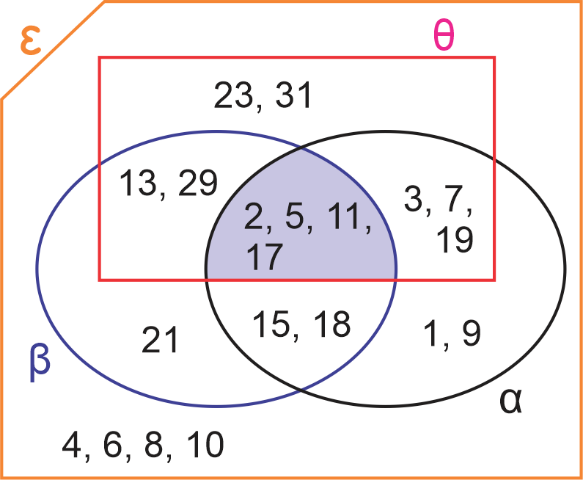
\includegraphics[width=0.7\textwidth]{figures/activity1-1.png}
  \end{center}

  \item List the elements in $\alpha$, $\beta$ and $\theta$.
  \item List the elements in $\alpha'$, $\beta'$ and $\theta'$.
  \item Find (a) $(\alpha \cup \beta \cup \theta)'$ \quad (b) $\alpha' \cap \beta' \cap \theta'$ \quad (c) $(\alpha \cap \beta \cap \theta)'$ \quad (d) $\alpha' \cup \beta' \cup \theta'$.
  \item Compare your result in 4(a) to 4(b). What conclusion can you draw?
  \item Compare your result in 4(c) to 4(d). What conclusion can you draw?
\end{enumerate}
\end{activity}

Compare your answer to the suggested solution below.

\begin{enumerate}[start=2]
  \item
  \begin{align*}
    \alpha &= \{1, 2, 3, 5, 7, 9, 11, 15, 17, 18, 19\}, \\
    \beta &= \{2, 5, 11, 13, 15, 17, 18, 21, 29\}, \\
    \theta &= \{2, 3, 5, 7, 11, 13, 17, 19, 23, 29, 31\}.
  \end{align*}
  \item
  \begin{align*}
    \alpha' &= \{4, 6, 8, 10, 13, 21, 23, 29, 31\}, \\
    \beta' &= \{1, 3, 4, 6, 7, 8, 9, 10, 19, 23, 31\}, \\
    \theta' &= \{1, 4, 6, 8, 9, 10, 15, 18, 21\}.
  \end{align*}
  \item
  \begin{align*}
    \text{(a)}\quad (\alpha \cup \beta \cup \theta)' &= \{4, 6, 8, 10\} \\
    \text{(b)}\quad \alpha' \cap \beta' \cap \theta' &= \{4, 6, 8, 10\} \\
    \text{(c)}\quad (\alpha \cap \beta \cap \theta)' &= \{1, 3, 4, 6, 8, 9, 10, 13, 19, 21, 23, 29, 31\} \\
    \text{(d)}\quad \alpha' \cup \beta' \cup \theta' &= \{1, 3, 4, 6, 8, 9, 10, 13, 19, 21, 23, 29, 31\}
  \end{align*}
  \item Results in 4(a) and 4(b) are equal. This confirms De Morgan's Law.
  \item Results in 4(c) and 4(d) are equal. This confirms De Morgan's Law.
\end{enumerate}

\begin{example}{Example 1.1}
Study the diagram carefully and use it to answer the questions.

\begin{center}
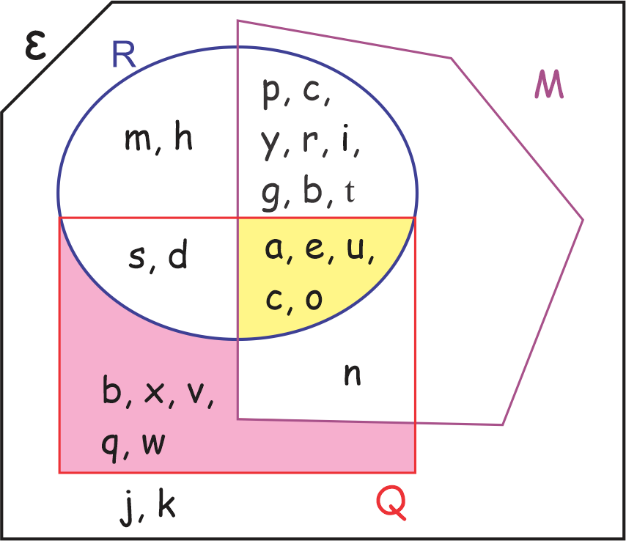
\includegraphics[width=0.65\textwidth]{figures/example1-1.png}
\end{center}

\begin{enumerate}
  \item List the elements in $R$, $M$, $Q$ and $\varepsilon$.
  \item Show that $R' \cap M' = (R \cup M)'$.
  \item Show that $(R \cap M \cap Q)' = R' \cup M' \cup Q'$.
\end{enumerate}
\medskip\noindent\textbf{Solution}
\begin{enumerate}
  \item
  \begin{align*}
    R &= \{s, u, b, d, e, r, m, a, t, o, g, l, y, p, h, i, c\}, \\
    M &= \{u, n, c, o, p, y, r, i, g, h, t, a, b, l, e\} \text{ and} \\
    Q &= \{a, e, u, c, o, n, x, q, v, w\} \text{ are subsets of} \\
    \varepsilon &= \{s, u, b, d, e, r, m, a, t, o, g, l, y, p, h, i, c, n, x, q, v, w, j, k\}.
  \end{align*}
  \item $R' \cap M' = (R \cup M)'$

  Let us first solve for $R' \cap M'$:
  \[
    \{b, x, v, n, q, w, j, k\} \cap \{m, h, s, d, b, x, v, q, w, j, k\}
  \]
  \[
    R' \cap M' = \{b, x, v, q, w, j, k\} \quad \ldots\ldots (1)
  \]
  Next, let us solve for $(R \cup M)'$:
  \[
    (R \cup M)' = \{s, u, b, d, e, r, m, a, t, o, g, l, y, p, h, i, c, n\}'
  \]
  \[
    (R \cup M)' = \{b, x, v, q, w, j, k\} \quad \ldots\ldots (2)
  \]
  Since equation (1) is equal to equation (2), it shows that $R' \cap M' = (R \cup M)'$.

  \booknote[S1-01]{the original textbook's working reproduced above actually
  contains an arithmetic slip --- from the given $R$, $M$ and $\varepsilon$,
  the correct complements are $R' = \{j,k,n,q,v,w,x\}$ and
  $M' = \{d,j,k,m,q,s,v,w,x\}$ \emph{(no `b' or `h')}, giving
  $R'\cap M' = (R\cup M)' = \{j,k,q,v,w,x\}$ rather than the $\{b,x,v,q,w,j,k\}$
  shown above. The error appears on both sides of the equation, so it does
  not affect the conclusion that $R'\cap M'=(R\cup M)'$, but the specific set
  of elements shown is incorrect.}

  \item Let's first solve for $(R \cap M \cap Q)'$:
  \[
    (R \cap M \cap Q)' = (a, e, u, c, o)'
  \]
  \[
    = \{s, b, d, r, m, t, g, l, y, p, h, i, n, x, q, v, w, j, k\} \quad \ldots\ldots (1)
  \]
  Next, let's find $R' \cup M' \cup Q'$:
  \begin{align*}
    R' \cup M' \cup Q' &= \{b, x, v, n, q, w, j, k\} \cup \{m, h, s, d, b, x, v, q, w, j, k\} \\
    &\quad \cup \{m, h, p, c, y, r, i, g, b, t, j, k\} \\
    &= \{s, b, d, r, m, t, g, l, y, p, h, i, n, x, q, v, w, j, k\} \quad \ldots\ldots (2)
  \end{align*}
  Since equation (1) is equal to equation (2), it shows $(R \cap M \cap Q)' = R' \cup M' \cup Q'$.

  \booknote[S1-02]{this working carries the same erroneous $R'$ and $M'$ from
  part 2, plus a similarly erroneous
  $Q' = \{b,c,g,h,i,j,k,m,p,r,t,y\}$ instead of the correct
  $Q' = \{b,d,g,h,i,j,k,l,m,p,r,s,t,y\}$ \emph{(no `c'; includes `d', `l', `s')}.
  Taking the union of the textbook's own three (erroneous) complements gives
  $\{b,c,d,g,h,i,j,k,m,n,p,q,r,s,t,v,w,x,y\}$ --- note the `c' --- not the
  $\{s,b,d,r,m,t,g,l,y,p,h,i,n,x,q,v,w,j,k\}$ (with an `l' instead of a `c')
  printed above, so the final line does not even follow from the textbook's
  own stated $R'$, $M'$, $Q'$. The correct result, computed directly from
  $R\cap M\cap Q=\{a,c,e,o,u\}$, is
  $(R\cap M\cap Q)' = \varepsilon\setminus\{a,c,e,o,u\}
  = \{b,d,g,h,i,j,k,l,m,n,p,q,r,s,t,v,w,x,y\}$, which does agree with
  $R'\cup M'\cup Q'$ once the correct complements from the note above are
  used instead. As before, the identity itself still holds; only the
  specific elements printed in the textbook's arithmetic are unreliable.}
\end{enumerate}
\end{example}

\section{Applying De Morgan's Laws of Set Theory}

We have learned about De Morgan's Laws of Set Theory. Now, we will look at its
application. Before we consider this application, let's familiarise ourselves with a
few properties of complements as it will be central to our understanding.

\subsection*{Properties of Complement}
\begin{enumerate}
  \item \textbf{Union of a set and its complement.} The union of a set $A$ and its complement ($A'$) is equal to the universal set ($\mu$), i.e.\ $A \cup A' = \mu$.
  \item \textbf{Intersection of a set and its complement.} The intersection of a set $A$ and its complement ($A'$) is equal to the null set ($\varnothing$), i.e.\ $A \cap A' = \{\ \} = \phi$.
  \item \textbf{Double complement.} The complement of the complement of set $A$ will give the same set, $A$, i.e.\ $(A')' = A$.
  \item \textbf{Complement of an empty set.} The complement of an empty set ($\phi$) is equal to the universal set ($\mu$), i.e.\ $\phi' = \mu$.
  \item \textbf{Complement of a universal set.} The complement of the universal set is equal to the null set, i.e.\ $\mu' = \phi$.
\end{enumerate}

\begin{example}{Example 1.2}
Rewrite: \quad a. $(X' \cup Y)'$ \qquad b. $(X \cap Y')'$

\medskip\noindent\textbf{Solution}
\begin{enumerate}
  \item[a.] $(X' \cup Y)'$

  Recall that from De Morgan's laws, we have $(A \cup B)' = A' \cap B'$.
  So, for $(X' \cup Y)'$, we will replace $A$ with $X'$ and $B$ with $Y$.
  This implies $(X' \cup Y)' = (X')' \cap Y'$.
  From the double complement property, $(X')' = X$.
  Therefore, $(X' \cup Y)' = X \cap Y'$.

  \item[b.] $(X \cap Y')'$

  Recall that from De Morgan's laws, we have $(A \cap B)' = A' \cup B'$.
  So, for $(X \cap Y')'$, we will replace $A$ with $X$ and $B$ with $Y'$.
  This implies $(X \cap Y')' = X' \cup (Y')'$.
  From the double complement property, $(Y')' = Y$.
  Therefore, $(X \cap Y')' = X' \cup Y$.
\end{enumerate}
\end{example}

\begin{example}{Example 1.3}
Show that:
\begin{enumerate}
  \item[a.] $(A \cup B' \cup C')' = A' \cap B \cap C$
  \item[b.] $(A' \cap B \cap C')' = A \cup B' \cup C$
\end{enumerate}

\medskip\noindent\textbf{Solution}
\begin{enumerate}
  \item[a.] Recall that $(A \cup B \cup C)' = A' \cap B' \cap C'$.
  This means, $(A \cup B' \cup C')' = A' \cap (B')' \cap (C')' = A' \cap B \cap C$.

  \item[b.] Recall that $(A \cap B \cap C)' = A' \cup B' \cup C'$.
  So, $(A' \cap B \cap C')' = (A')' \cup B' \cup (C')' = A \cup B' \cup C$.
\end{enumerate}
\end{example}

\begin{example}{Example 1.4}
Rewrite $\big[(P \cup Q')' \cap P\big]'$.

\medskip\noindent\textbf{Solution}

\textbf{Method 1} --- Let us start with the outer bracket.

Using $[A \cap B]' = A' \cup B'$:
\[
  \big[(P \cup Q')' \cap P\big]' = (P \cup Q')'' \cup P' = (P \cup Q') \cup P'
\]
Since the union is commutative, $P \cup Q' = Q' \cup P$:
\[
  \big[(P \cup Q')' \cap P\big]' = (Q' \cup P) \cup P'
\]
Since the union of sets is associative, $(Q' \cup P) \cup P' = Q' \cup (P \cup P')$:
\[
  \big[(P \cup Q')' \cap P\big]' = Q' \cup (P \cup P')
\]
Recall that $P \cup P' = \mu$ (universal set):
\[
  \big[(P \cup Q')' \cap P\big]' = Q' \cup \mu = \mu
\]

\textbf{Method 2} --- We will start with the inner bracket and work our way out.
\[
  \big[(P \cup Q')' \cap P\big]'
\]
\[
  (P \cup Q')' = P' \cap Q'' = P' \cap Q
\]
\[
  \big[(P \cup Q')' \cap P\big]' = \big[(P' \cap Q) \cap P\big]'
\]
Since the intersection of sets is commutative, $P' \cap Q = Q \cap P'$:
\[
  \big[(P \cup Q')' \cap P\big]' = \big[(Q \cap P') \cap P\big]'
\]
Since intersection is associative, $(Q \cap P') \cap P = Q \cap (P' \cap P)$:
\[
  \big[(P \cup Q')' \cap P\big]' = \big[Q \cap (P' \cap P)\big]'
\]
Recall that $P' \cap P = \varnothing$:
\[
  \big[(P \cup Q')' \cap P\big]' = [Q \cap \varnothing]' = [\varnothing]' = \mu
\]
\end{example}

\begin{example}{Example 1.5}
Using the Venn diagram, shade the region represented by:
\begin{enumerate}
  \item[a.] $(X \cup Y)' \cap Z$
  \item[b.] $X' \cap (Y \cup Z)$
\end{enumerate}

\medskip\noindent\textbf{Solution}

\textbf{a. $(X \cup Y)' \cap Z$}

Since the expression involves three sets, $X$, $Y$ and $Z$, we will construct a
three-set Venn diagram. We will represent the universal set with $\mu$. An example
is shown below:

\begin{center}
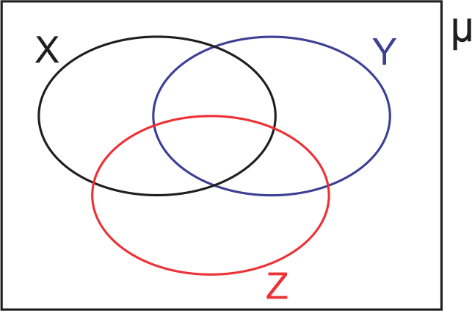
\includegraphics[width=0.55\textwidth]{figures/example1-5-blank.png}
\end{center}

$(X \cup Y)'$ represents elements which are not in $X \cup Y$. We use vertical
lines to shade this region:

\begin{center}
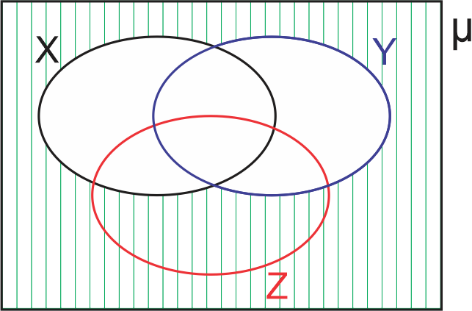
\includegraphics[width=0.55\textwidth]{figures/example1-5-vertical.png}
\end{center}

Then, on the same diagram, set $Z$ is shaded with horizontal lines. The
intersection of $(X \cup Y)'$ and $Z$ is the double-shaded (cross-hatched) area:

\begin{center}
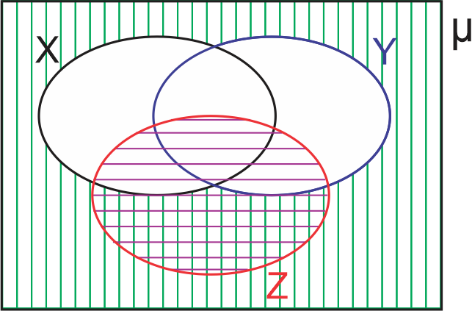
\includegraphics[width=0.55\textwidth]{figures/example1-5-combined.png}
\end{center}

Therefore, $(X \cup Y)' \cap Z$ is the region shown below, shaded in a single
cross-hatch pattern:

\begin{center}
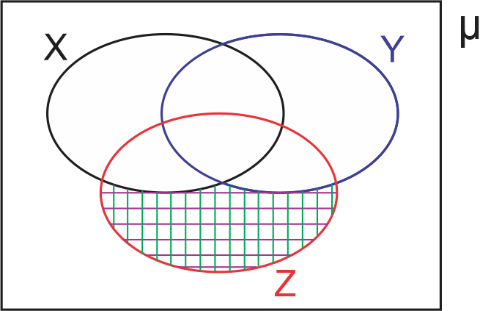
\includegraphics[width=0.55\textwidth]{figures/example1-5-final.png}
\end{center}

\textbf{b. $X' \cap (Y \cup Z)$} is found in the same way: shade $X'$ (everything outside
circle $X$) with vertical lines, shade $Y \cup Z$ with horizontal lines, and the
region shaded by both patterns is the required set.
\end{example}

In year 1, we learned about set theory laws. Examples of these laws include
commutative, associative and distributive. We also learned to identify the regions
in a three-set Venn diagram. In this lesson, we will apply these concepts to answer
real-life problems.

\subsection*{How to complete a three-set Venn diagram}
\begin{enumerate}
  \item Start with the intersection of the three sets and proceed to the regions
  involving two sets.
  \item Then work on the regions involving one set and finally the regions in the
  universal set that do not intersect with any of the three sets.
\end{enumerate}
To summarise, start from the centre (the region with the most overlaps) and work
your way out.

\begin{example}{Example 1.6}
Set $A = \{\text{odd numbers less than } 15\}$

Set $B = \{W : 4 < W \le 11\}$

Set $D = \{\text{Prime numbers less than } 14\}$

All of which are subsets of Set $R = \{0, 1, 2, 3, 4, \ldots, 16\}$.
\begin{enumerate}
  \item[a.] List the members of the following sets: (i) $A$ \quad (ii) $B$ \quad (iii) $D$ \quad (iv) $A \cup B$ \quad (v) $(A \cup B) \cap D'$ \quad (vi) $(A' \cap B) \cup D$.
  \item[b.] Represent $A$, $B$, $D$ and $R$ using a Venn diagram.
\end{enumerate}

\medskip\noindent\textbf{Solution}
\begin{enumerate}
  \item[a.]
  \begin{align*}
    \text{(i)}\quad A &= \{1, 3, 5, 7, 9, 11, 13\} \\
    \text{(ii)}\quad B &= \{5, 6, 7, 8, 9, 10, 11\} \\
    \text{(iii)}\quad D &= \{2, 3, 5, 7, 11, 13\} \\
    \text{(iv)}\quad A \cup B &= \{1, 3, 5, 7, 9, 11, 13\} \cup \{5, 6, 7, 8, 9, 10, 11\} \\
    &= \{1, 3, 5, 6, 7, 8, 9, 10, 11, 13\} \\
    \text{(v)}\quad (A \cup B) \cap D' &= \{1, 3, 5, 6, 7, 8, 9, 10, 11, 13\} \cap \{1, 4, 6, 8, 9, 10, 12, 14, 15, 16\} \\
    &= \{1, 6, 8, 9, 10\} \\
    \text{(vi)}\quad A' \cap B &= \{2, 4, 6, 8, 10, 12, 14, 15, 16\} \cap \{5, 6, 7, 8, 9, 10, 11\} = \{6, 8, 10\} \\
    (A' \cap B) \cup D &= \{6, 8, 10\} \cup \{2, 3, 5, 7, 11, 13\} = \{2, 3, 5, 6, 7, 8, 10, 11, 13\}
  \end{align*}

  \item[b.] We first find the triple intersection: $A \cap B \cap D = \{5, 7, 11\}$.

  \begin{center}
  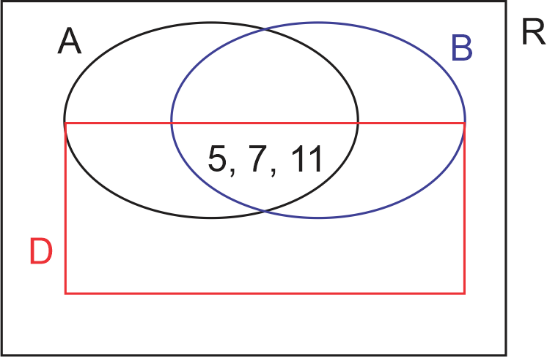
\includegraphics[width=0.55\textwidth]{figures/example1-6-triple.png}
  \end{center}

  Then proceed to the pairwise intersections. There are three of these:
  \begin{align*}
    A \cap B \text{ only} &= A \cap B \cap D' = \{9\} \\
    A \cap D \text{ only} &= A \cap B' \cap D = \{3, 13\} \\
    B \cap D \text{ only} &= A' \cap B \cap D = \{\ \}
  \end{align*}
  Let's update our diagram with these values:

  \begin{center}
  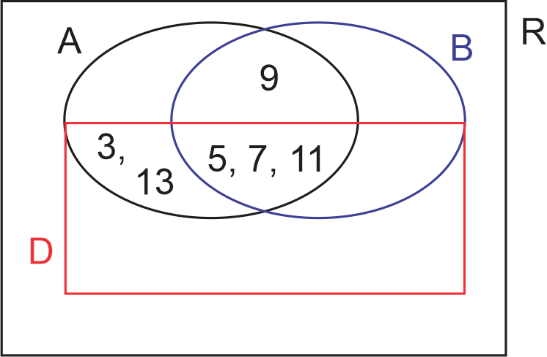
\includegraphics[width=0.55\textwidth]{figures/example1-6-pairwise.png}
  \end{center}

  Next, find the single intersections. There are three of them:
  \begin{align*}
    A \text{ only} &= \{1\} \\
    B \text{ only} &= \{6, 8, 10\} \\
    D \text{ only} &= \{2\}
  \end{align*}

  \begin{center}
  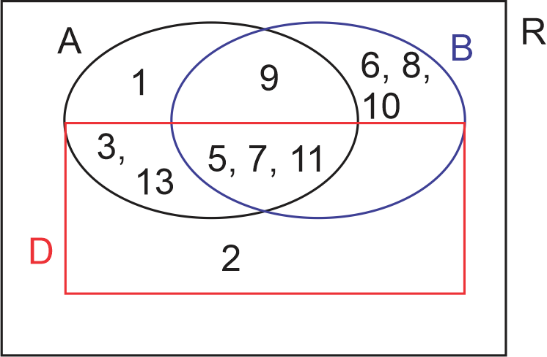
\includegraphics[width=0.55\textwidth]{figures/example1-6-singles.png}
  \end{center}

  Finally, we find $(A \cup B \cup D)' = \{0, 4, 12, 14, 15, 16\}$.

  Find below the completed diagram:
  \begin{center}
  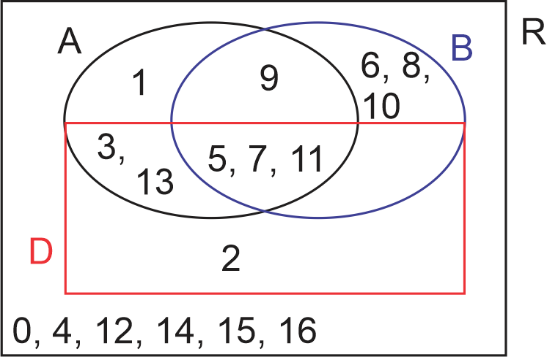
\includegraphics[width=0.55\textwidth]{figures/example1-6-completed.png}
  \end{center}
\end{enumerate}
\end{example}

\begin{example}{Example 1.7}
A survey of 70 investors reveals the following: 30 invest in bonds, 40 in stocks
and 21 in annuities. 10 had investments in bonds and annuities, 15 in bonds and
stocks, 12 in stocks and annuities, and 7 had investments in all three assets. The
remaining investors had investments in other assets.

Create a Venn diagram for this information.

\medskip\noindent\textbf{Solution}

First, draw a Venn diagram with three intersecting sets representing the three
main sets: Bonds, Stocks, and Annuities. Let $B$ represent Bonds, $A$ represent
Annuities and $S$ represent Stocks. This means $n(B) = 30$, $n(A) = 21$ and
$n(S) = 40$.

\begin{center}
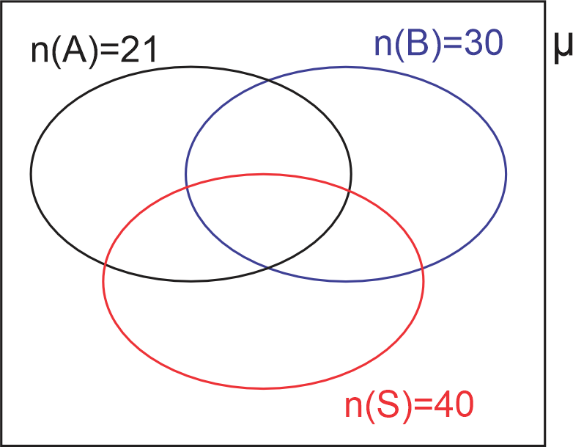
\includegraphics[width=0.5\textwidth]{figures/example1-7-blank.png}
\end{center}

Next, we fill in the region where all three sets intersect. From the question,
this figure is 7.

\begin{center}
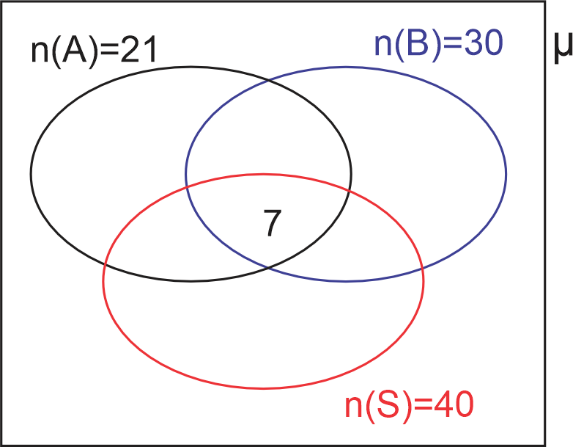
\includegraphics[width=0.5\textwidth]{figures/example1-7-triple.png}
\end{center}

Let us add these values to the Venn diagram. Next, we fill in the regions where
exactly two sets intersect:
\begin{enumerate}
  \item[a.] \textbf{Bonds and Annuities.} A total of 10 had investments in bonds and
  annuities but 7 of them have investments in all three assets. This leaves
  $10 - 7 = 3$ investing in only Bonds and Annuities.
  \item[b.] \textbf{Bonds and Stocks.} A total of 15 had investments in bonds and
  stocks but 7 of them had investments in all three assets. This leaves
  $15 - 7 = 8$ investing in only Bonds and Stocks.
  \item[c.] \textbf{Stocks and Annuities.} A total of 12 had investments in stocks and
  annuities but 7 of them have investments in all three assets. This leaves
  $12 - 7 = 5$ investing in only Stocks and Annuities.
\end{enumerate}

\begin{center}
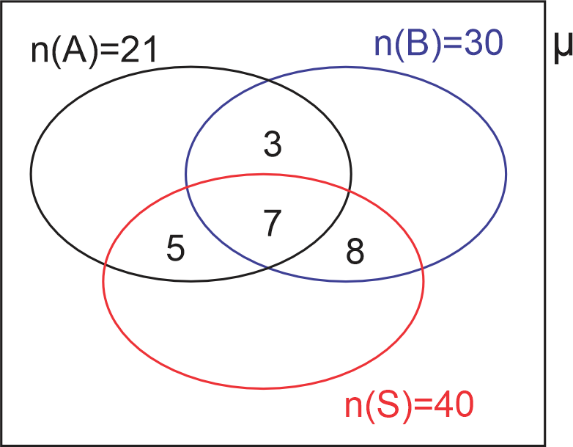
\includegraphics[width=0.5\textwidth]{figures/example1-7-pairwise.png}
\end{center}

You will realise there is only one region remaining in each set. These are the
regions that represent only one set:
\begin{enumerate}
  \item[a.] \textbf{Only Bonds.} A total of 30 had investments in bonds but we have
  already accounted for $3 + 7 + 8 = 18$ of them, leaving $30 - 18 = 12$ having
  investments in only Bonds.
  \item[b.] \textbf{Only Annuities.} A total of 21 had investments in annuities but we
  have already accounted for $3 + 7 + 5 = 15$ of them, leaving $21 - 15 = 6$
  having investments in only Annuities.
  \item[c.] \textbf{Only Stocks.} A total of 40 had investments in stocks but we have
  already accounted for $5 + 7 + 8 = 20$ of them, leaving $40 - 20 = 20$
  investing in only Stocks.
\end{enumerate}

We will add these values to the Venn diagram:

\begin{center}
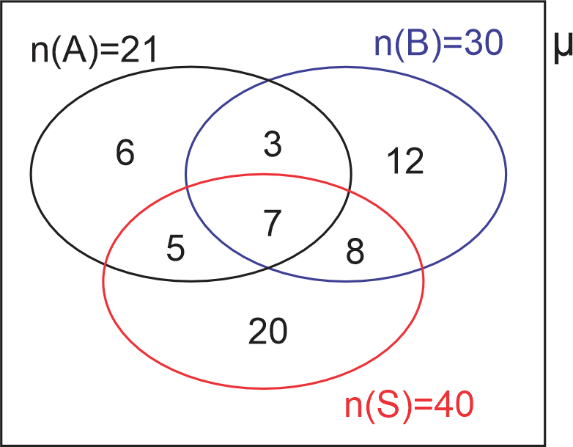
\includegraphics[width=0.5\textwidth]{figures/example1-7-singles.png}
\end{center}

Finally, we calculate the number of investors with no investments in the three
assets. The sum of all the values already calculated for the intersecting sets is
\[
  12 + 3 + 6 + 8 + 5 + 7 + 20 = 61.
\]
This means $70 - 61 = 9$ investors did not invest in any of the three assets. This
value is recorded outside the circles but inside the universal set, completing the
Venn diagram:

\begin{center}
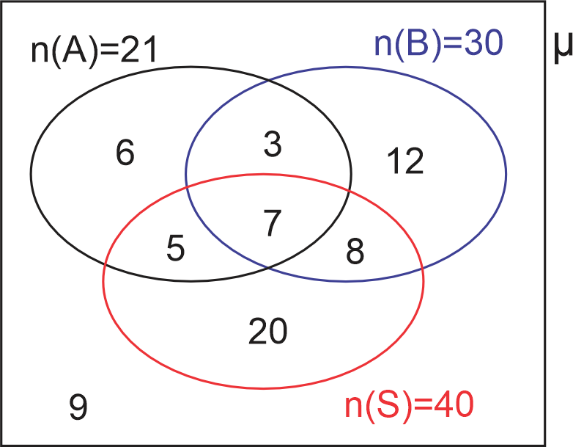
\includegraphics[width=0.55\textwidth]{figures/example1-7-completed.png}
\end{center}
\end{example}

\begin{example}{Example 1.8}
A survey of 97 countries that participated in the Olympics reveals that 80 won
bronze, 57 won silver and 47 won gold. It also reveals that 30 won gold and
silver, 50 won silver and bronze, 38 won gold and bronze, and 3 countries did not
win any medal.
\begin{enumerate}
  \item[a.] Illustrate the information on a Venn diagram.
  \item[b.] Calculate the number of countries who won all three medals.
  \item[c.] Calculate the number of countries who won exactly two medals.
\end{enumerate}

\medskip\noindent\textbf{Solution}

Let $B$ = Bronze medal, $G$ = Gold medal, and $S$ = Silver medal, so
$n(B) = 80$, $n(S) = 57$ and $n(G) = 47$.

Let $x$ be the number of countries who won all three medals (unknown, since we
were not given this directly).

\begin{center}
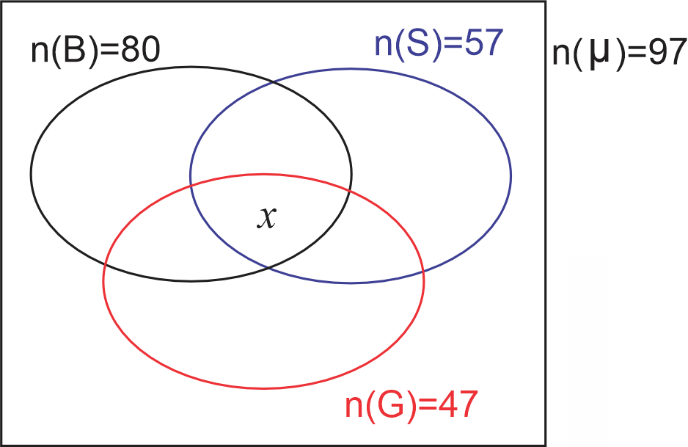
\includegraphics[width=0.5\textwidth]{figures/example1-8-blank.png}
\end{center}

Next, we fill in the regions where exactly two sets intersect (countries that won
exactly two of the three medals). A total of 30 countries won Gold and Silver;
of these, $x$ won all three medals, so $(30-x)$ countries won \emph{only} Gold and
Silver. Similarly, 50 won Silver and Bronze, giving $(50 - x)$ who won only
Silver and Bronze, and 38 won Gold and Bronze, giving $(38-x)$ who won only
Gold and Bronze.

\begin{center}
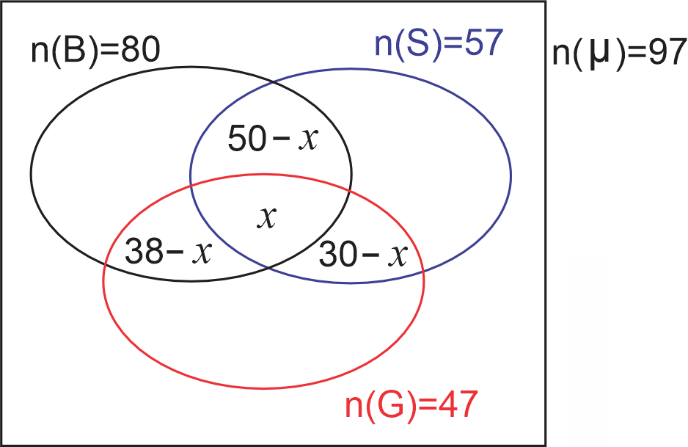
\includegraphics[width=0.5\textwidth]{figures/example1-8-pairwise.png}
\end{center}

At this point only one region remains in each set:
\begin{itemize}
  \item \textbf{Only Bronze.} $80$ won bronze, and we have already accounted for
  $x + (50-x) + (38-x) = (88-x)$ of them, leaving $80 - (88-x) = (x - 8)$
  winning only bronze.
  \item \textbf{Only Silver.} $57$ won silver, and we have already accounted for
  $x + (50-x) + (30-x) = (80-x)$ of them, leaving $57 - (80-x) = (x - 23)$
  winning only silver.
  \item \textbf{Only Gold.} $47$ won gold, and we have already accounted for
  $x + (30-x) + (38-x) = (68-x)$ of them, leaving $47 - (68-x) = (x - 21)$
  winning only gold.
\end{itemize}

\begin{center}
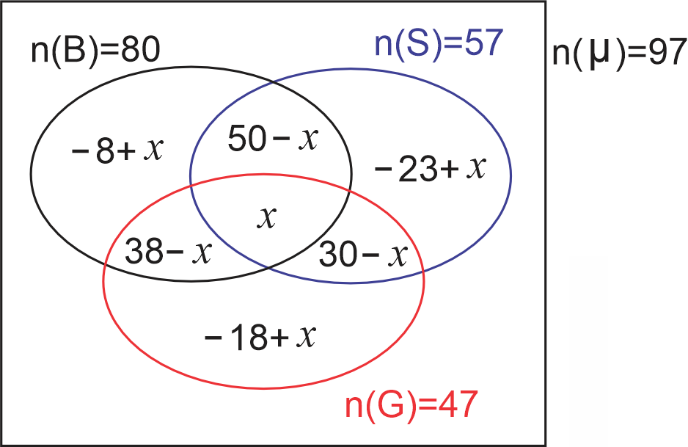
\includegraphics[width=0.5\textwidth]{figures/example1-8-singles.png}
\end{center}

\booknote[S1-03]{the Gold-only region in this diagram is labelled $-18+x$ in the
original textbook figure --- this is a typo. As derived above, the correct
formula is $x-21$. We use the correct formula going forward.}

According to the question, 3 countries did not win any medal, so
$(G \cup S \cup B)' = 3$.

\begin{center}
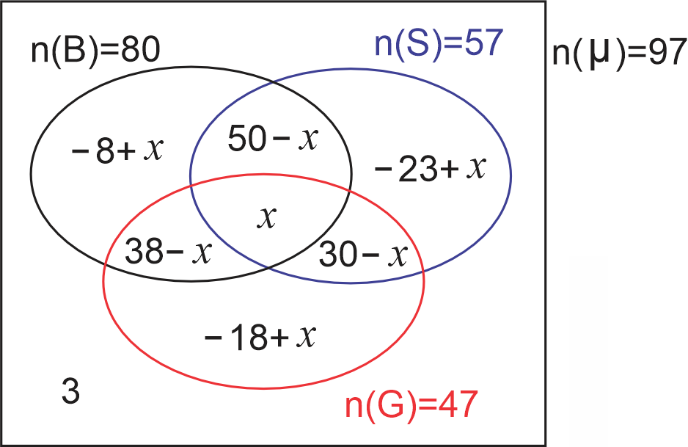
\includegraphics[width=0.5\textwidth]{figures/example1-8-nomedal.png}
\end{center}

To solve for $x$, add all the entries and equate the result to the total number of
countries under consideration (97):
\[
  x + (30-x) + (50-x) + (38-x) + (x-8) + (x-23) + (x-21) + 3 = 97
\]
\[
  x + 69 = 97 \implies x = 97 - 69 = 28.
\]

\begin{enumerate}
  \item[e.] Therefore, \textbf{28} countries won all three medals.
  \item[f.] Number of countries that won exactly two medals $= (30-28) + (50-28) + (38-28) = 2 + 22 + 10 = 34$.
\end{enumerate}

We can now update the diagram with this value. The completed Venn diagram, as
given in the original textbook, is:
\begin{center}
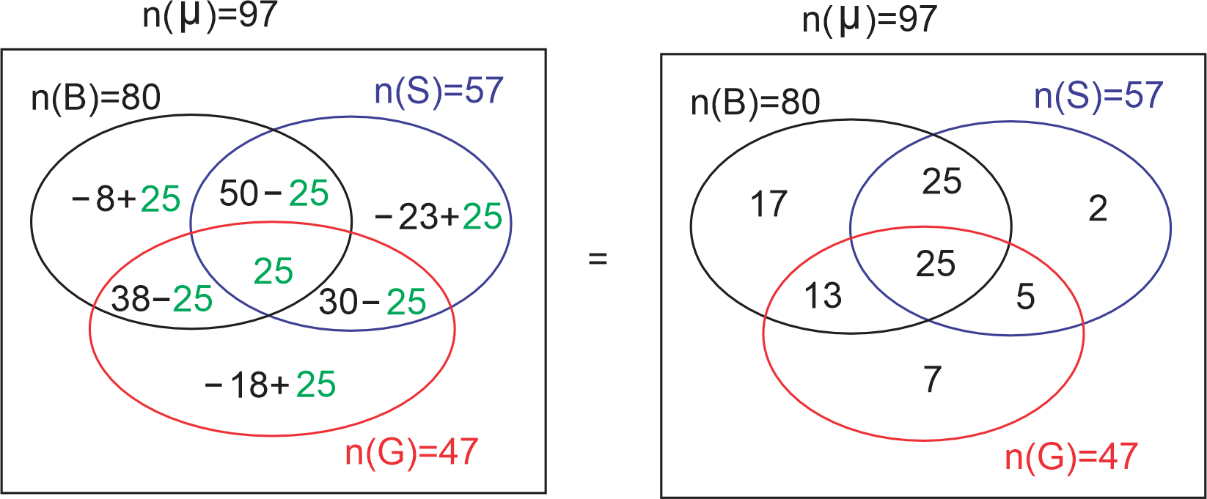
\includegraphics[width=0.85\textwidth]{figures/example1-8-final-book.png}
\end{center}

\booknote[S1-04]{the textbook substitutes $x=25$ into the region
formulas above, not the value $x=28$ that was just solved for algebraically.
This is an error in the original --- every region value shown (17, 25, 2, 13,
25, 5) other than the Gold-only region is inconsistent with $x=28$, and the
diagram's own values do not agree with part (f)'s answer of 34 for the number
of countries winning exactly two medals ($25+13+5=43\neq34$, using the
diagram's own printed numbers). Substituting the correctly-solved $x=28$
into each formula instead gives Bronze-only $=x-8=20$,
Bronze$\cap$Silver-only $=50-x=22$, Silver-only $=x-23=5$,
Bronze$\cap$Gold-only $=38-x=10$, Silver$\cap$Gold-only $=30-x=2$, and
Gold-only $=x-21=7$ (triple intersection $=28$), which does check against
part (f): $2+22+10=34$.}
\end{example}

\section{Expanding Binomial Expressions}

Hopefully you recall the work we did in Year 1 on the binomial expansion. We
used the Pascal triangle and the Combination method to expand and simplify
certain expressions. Let's remind you of this in the activity below.

\begin{activity}{Activity 1.2: Revision}
\begin{enumerate}
  \item In groups or pairs, write down or generate the Pascal triangle up to $(x+y)^5$.
  \item Use your results in step 1 to simplify the expressions:
  \begin{enumerate}
    \item[a.] $(2x+y)^3$
    \item[b.] $(a-3b)^4$
    \item[c.] $(2+\sqrt{x})^5$
  \end{enumerate}
  \item Apply the combination method to also simplify the above tasks.
  \item Compare your results in (2) and (3) and write down any observations.
  \item Show your solutions, or write up, to classmates in other groups or to
  your mathematics teacher.
\end{enumerate}
\end{activity}

The Binomial Expansion helps us to expand and simplify complex expressions,
which would have been difficult using the idea of algebraic expressions. Under
algebraic expressions we could only expand with a positive integer power, but the
binomial theorem will help us to expand any expression with a rational number
as the power.

\begin{activity}{Activity 1.3 -- Derivation of Binomial Theorem}
\begin{enumerate}
  \item Look for the $^{n}C_{r}$ button on your calculator.
  \item Task: use $^{n}C_{r}$ on your calculator to evaluate
  \begin{enumerate}
    \item[i)] $^{3}C_{0}$
    \item[ii)] $^{3}C_{1}$
    \item[iii)] $^{3}C_{2}$
    \item[iv)] $^{3}C_{3}$
  \end{enumerate}
  \item Hopefully the answers you have are: $1\ 3\ 3\ 1$. This was used in Year 1 to
  expand certain expressions.
\end{enumerate}
\end{activity}

The combination of $n$ items taking $r$ at a time is:
\[
  \binom{n}{r} = {}^{n}C_{r} = \frac{n!}{(n-r)!\,r!}, \qquad \text{where } n! \text{ is read as ``}n\text{ factorial''}
\]
and is explained as $n! = n(n-1)(n-2)(n-3)\cdots 2 \times 1$.

For example, $5! = 5(5-1)(5-2)(5-3)(5-4) = 5 \times 4 \times 3 \times 2 \times 1 = 120$.

You could also find $5!$ using a calculator. Look for $!$ on your calculator to
find $5!$, to confirm the answer obtained above.

\begin{example}{Example 1.9}
In groups or in pairs, solve the following without using a calculator:
\begin{enumerate}
  \item[a.] $^{6}C_{3}$
  \item[b.] $^{4}C_{2}$
\end{enumerate}
Confirm your answers with a calculator.

\medskip\noindent\textbf{Solution}
\begin{enumerate}
  \item[a.] $^{6}C_{3} = \dfrac{6!}{(6-3)!\,3!} = \dfrac{6\times5\times4\times3\times2\times1}{3\times2\times1\times3\times2\times1} = \dfrac{6\times5\times4}{3\times2\times1} = \dfrac{120}{6} = 20$
  \item[b.] $^{4}C_{2} = \dfrac{4!}{(4-2)!\,2!} = \dfrac{4\times3\times2\times1}{2\times1\times2\times1} = \dfrac{4\times3}{2\times1} = \dfrac{12}{2} = 6$
\end{enumerate}
\end{example}

\begin{activity}{Activity 1.4: General Form of Binomial Theorem}
\begin{enumerate}
  \item Using the definition $\binom{n}{r} = {}^{n}C_{r} = \dfrac{n!}{(n-r)!\,r!}$, work in pairs or
  groups and discuss how the following evaluations were done:
  \begin{enumerate}
    \item[a.] ${}^{n}C_{1} = \dfrac{n!}{(n-1)!\times 1!} = \dfrac{n(n-1)!}{(n-1)!\times 1} = n$
    \item[b.] ${}^{n}C_{2} = \dfrac{n!}{(n-2)!\times 2!} = \dfrac{n(n-1)(n-2)!}{(n-2)!\times 2\times 1} = \dfrac{n(n-1)}{2}$
    \item[c.] ${}^{n}C_{3} = \dfrac{n!}{(n-3)!\times 3!} = \dfrac{n(n-1)(n-2)(n-3)!}{(n-3)!\times 3\times 2\times 1} = \dfrac{n(n-1)(n-2)}{6}$
  \end{enumerate}
  \item Write down your challenges or observations for a class discussion with
  your classmates and teacher.
\end{enumerate}
\end{activity}

It must be noted that ${}^{n}C_{0} = 1$ and $0! = 1$.

In general, the Binomial Theorem is written as:
\[
  (a+x)^n = {}^{n}C_{0}\,a^n x^0 + {}^{n}C_{1}\,a^{n-1}x^1 + {}^{n}C_{2}\,a^{n-2}x^2 + {}^{n}C_{3}\,a^{n-3}x^3 + \cdots + {}^{n}C_{r}\,a^{n-r}x^r + \cdots + {}^{n}C_{n}\,a^0 x^n
\]
\[
  = a^n + n\,a^{n-1}x + \frac{n(n-1)}{2!}\,a^{n-2}x^2 + \frac{n(n-1)(n-2)}{3!}\,a^{n-3}x^3 + \cdots + x^n
\]

There is a special case when $a = 1$. Substituting $a=1$:
\[
  (1+x)^n = 1 + nx + \frac{n(n-1)}{2!}x^2 + \frac{n(n-1)(n-2)}{3!}x^3 + \cdots + x^n
\]

Let us go through the following worked examples to assist us in the expansion
of the form $(1-x)^n$ or $(1+x)^n$.

\begin{example}{Example 1.10}
By using the Binomial Theorem, fully expand the expression $(1+x)^5$.

\medskip\noindent\textbf{Solution}

Using the binomial theorem,
\[
  (1+x)^n = 1 + nx + \frac{n(n-1)}{2!}x^2 + \frac{n(n-1)(n-2)}{3!}x^3 + \cdots + x^n
\]
In this case $n=5$, so we substitute this in:
\[
  (1+x)^5 = 1 + 5x + \frac{5\times4}{2!}x^2 + \frac{5\times4\times3}{3!}x^3 + \frac{5\times4\times3\times2}{4!}x^4 + x^5
\]
Simplify the coefficients to obtain:
\[
  = 1 + 5x + \frac{5\times4}{2\times1}x^2 + \frac{5\times4\times3}{3\times2\times1}x^3 + \frac{5\times4\times3\times2}{4\times3\times2\times1}x^4 + x^5
\]
\[
  = 1 + 5x + 10x^2 + 10x^3 + 5x^4 + x^5
\]
\end{example}

\begin{example}{Example 1.11}
By using the Binomial Theorem, fully expand the expression $(1+2x)^4$.

\medskip\noindent\textbf{Solution}

Using the binomial theorem $(1+x)^n = 1 + nx + \frac{n(n-1)}{2!}x^2 + \frac{n(n-1)(n-2)}{3!}x^3 + \cdots + x^n$,
in this case $n=4$ and `$x$' $=2x$, so we substitute these in:
\[
  (1+2x)^4 = 1 + 4(2x) + \frac{4\times3}{2!}(2x)^2 + \frac{4\times3\times2}{3!}(2x)^3 + (2x)^4
\]
Simplify the coefficients to obtain:
\[
  = 1 + 4(2x) + \frac{4\times3}{2\times1}\times 4x^2 + \frac{4\times3\times2}{3\times2\times1}\times 8x^3 + 16x^4
\]
\[
  = 1 + 8x + 24x^2 + 32x^3 + 16x^4
\]
\end{example}

\begin{example}{Example 1.12}
Find the first four terms of the binomial $\sqrt{1+2x}$ using the binomial theorem.

\medskip\noindent\textbf{Solution}
\[
  \sqrt{1+2x} = (1+2x)^{1/2}
\]
In this case $n = \tfrac{1}{2}$ and `$x$' $=2x$, so we substitute these in:
\[
  (1+2x)^{1/2} = 1 + \tfrac{1}{2}(2x) + \frac{\tfrac{1}{2}\left(\tfrac{1}{2}-1\right)}{2!}(2x)^2 + \frac{\tfrac{1}{2}\left(\tfrac{1}{2}-1\right)\left(\tfrac{1}{2}-2\right)}{3!}(2x)^3
\]
\[
  = 1 + \tfrac{1}{2}(2x) + \frac{\tfrac{1}{2}\left(-\tfrac{1}{2}\right)}{2\times1}(4x^2) + \frac{\tfrac{1}{2}\left(-\tfrac{1}{2}\right)\left(-\tfrac{3}{2}\right)}{3\times2\times1}(8x^3)
\]
\[
  = 1 + x - \tfrac{1}{2}x^2 + \tfrac{1}{2}x^3
\]
\end{example}

\begin{example}{Example 1.13}
Find the first four terms of the binomial $\sqrt[3]{1-3x}$ using the binomial theorem.

\medskip\noindent\textbf{Solution}
\[
  \sqrt[3]{1-3x} = (1-3x)^{1/3}
\]
In this case $n = \tfrac{1}{3}$ and `$x$' $=-3x$, so we substitute these in:
\[
  (1-3x)^{1/3} = 1 + \tfrac{1}{3}(-3x) + \frac{\tfrac{1}{3}\left(\tfrac{1}{3}-1\right)}{2!}(-3x)^2 + \frac{\tfrac{1}{3}\left(\tfrac{1}{3}-1\right)\left(\tfrac{1}{3}-2\right)}{3!}(-3x)^3
\]
\[
  = 1 + \tfrac{1}{3}(-3x) + \frac{\tfrac{1}{3}\left(-\tfrac{2}{3}\right)}{2\times1}(-3x)^2 + \frac{\tfrac{1}{3}\left(-\tfrac{2}{3}\right)\left(-\tfrac{5}{3}\right)}{3\times2\times1}(-3x)^3
\]
\[
  = 1 + \tfrac{1}{3}(-3x) + \frac{-\tfrac{2}{9}}{2}(9x^2) + \frac{\tfrac{10}{27}}{6}(-27x^3)
\]
\[
  = 1 - x - x^2 - \tfrac{5}{3}x^3
\]
\end{example}

\begin{example}{Example 1.14}
Expand up to the fifth term the expression $\dfrac{1}{(1-x)^2}$.

\medskip\noindent\textbf{Solution}

Rewriting $\dfrac{1}{(1-x)^2}$ using the rules of indices, $\dfrac{1}{(1-x)^2} = (1-x)^{-2}$.
\begin{align*}
  (1-x)^{-2} &= 1 - 2(-x) + \frac{-2(-2-1)}{2!}(-x)^2 + \frac{-2(-2-1)(-2-2)}{3!}(-x)^3 \\
  &\quad + \frac{-2(-2-1)(-2-2)(-2-3)}{4!}(-x)^4 \\
  &= 1 - 2(-x) + \frac{-2(-3)}{2\times1}(-x)^2 + \frac{-2(-3)(-4)}{3\times2\times1}(-x)^3 + \frac{-2(-3)(-4)(-5)}{4\times3\times2\times1}(-x)^4
\end{align*}
\[
  (1-x)^{-2} = 1 + 2x + 3x^2 + 4x^3 + 5x^4
\]
\end{example}

\begin{example}{Example 1.15}
Find the first four terms of $(1-16x)^{1/4}$.

\medskip\noindent\textbf{Solution}
\begin{align*}
  (1-16x)^{1/4} &= 1 + \tfrac{1}{4}(-16x) + \frac{\tfrac{1}{4}\left(\tfrac{1}{4}-1\right)}{2!}(-16x)^2 + \frac{\tfrac{1}{4}\left(\tfrac{1}{4}-1\right)\left(\tfrac{1}{4}-2\right)}{3!}(-16x)^3 \\
  &= 1 + \tfrac{1}{4}(-16x) + \frac{\tfrac{1}{4}\left(-\tfrac{3}{4}\right)}{2\times1}(-16x)^2 + \frac{\tfrac{1}{4}\left(-\tfrac{3}{4}\right)\left(-\tfrac{7}{4}\right)}{3\times2\times1}(-16x)^3 \\
  &= 1 + \tfrac{1}{4}(-16x) + \frac{-\tfrac{3}{16}}{2}(256x^2) + \frac{\tfrac{21}{64}}{6}(-4096x^3)
\end{align*}
\[
  = 1 - 4x - 24x^2 - 224x^3
\]
\end{example}

\begin{activity}{Activity 1.5: Deciding Whether the Binomial Theorem Can Be Used in All Cases}
Discuss in groups whether the binomial theorem
\[
  (1+x)^n = 1 + nx + \frac{n(n-1)}{2!}x^2 + \frac{n(n-1)(n-2)}{3!}x^3 + \cdots + x^n
\]
can be used in all cases.
\begin{enumerate}
  \item Consider $(2+4x)^4$. Can the binomial theorem be used directly?
  \item How will you write the terms in the bracket to have $1$ as one of the terms?
  \item Let us go through the following tasks to help us write $(2+4x)^4$ in the
  form $(1+x)^n$ and use the binomial theorem to expand and simplify:
  \begin{itemize}
    \item[] \textbf{Task 1:} Take the given binomial expression $(2+4x)$.
    \item[] \textbf{Task 2:} Factorise the constant out from the binomial to obtain $2(1+2x)$.
    \item[] \textbf{Task 3:} Rewrite your expression obtained with the power as given, i.e.\ $2^4(1+2x)^4$.
    \item[] \textbf{Task 4:} Expand the binomial $(1+2x)^4$, after which you multiply your result by $2^4$.
  \end{itemize}
  Now follow the tasks to obtain all the terms for the given expression.

  \textbf{Expected Answer:} $16 + 128x + 348x^2 + 512x^3 + 256x^4$.
\end{enumerate}
\end{activity}

Let's solve the following examples using the binomial theorem.

\begin{example}{Example 1.16}
\begin{enumerate}
  \item Use the binomial theorem to expand fully $(3+9x)^5$.
  \item Find the first three terms of $\left(\dfrac{4}{9}+6x\right)^{1/2}$ using the binomial theorem.
  \item Use the binomial theorem to expand fully and simplify $(10+4x)^3$.
  \item Use the binomial theorem to find the first four terms of the expression $\sqrt[4]{81+162x}$.
\end{enumerate}

\medskip\noindent\textbf{Solution}

\textbf{1.}
\[
  (3+9x)^5 = 3^5(1+3x)^5
\]
\begin{align*}
  3^5(1+3x)^5 &= 3^5\Bigg[1 + 5(3x) + \frac{5(4)}{2\times1}(3x)^2 + \frac{5(4)(3)}{3\times2\times1}(3x)^3 \\
  &\qquad + \frac{5(4)(3)(2)}{4\times3\times2\times1}(3x)^4 + \frac{5(4)(3)(2)(1)}{5\times4\times3\times2\times1}(3x)^5\Bigg]
\end{align*}
\[
  = 243\left[1 + 5(3x) + 10(9x^2) + 10(27x^3) + 5(81x^4) + (243x^5)\right]
\]
\[
  (3+9x)^5 = 243\left(1 + 15x + 90x^2 + 270x^3 + 405x^4 + 243x^5\right)
\]
Compute the final coefficients:
\begin{itemize}
  \item $243 \times 1 = 243$
  \item $243 \times 15 = 3645$
  \item $243 \times 90 = 21870$
  \item $243 \times 270 = 65610$
  \item $243 \times 405 = 98415$
  \item $243 \times 243 = 59049$
\end{itemize}
Therefore, the expansion is
\[
  (3+9x)^5 = 243 + 3645x + 21870x^2 + 65610x^3 + 98415x^4 + 59049x^5.
\]

\textbf{2.}
\[
  \left(\frac{4}{9}+6x\right)^{1/2} = \left(\frac{4}{9}\right)^{1/2}\left(1+\frac{27}{2}x\right)^{1/2}
\]
\[
  = \left(\frac{4}{9}\right)^{1/2}\left[1 + \frac{1}{2}\left(\frac{27}{2}x\right) + \frac{\tfrac{1}{2}\left(\tfrac{1}{2}-1\right)}{2!}\left(\frac{27}{2}x\right)^2\right]
\]
\[
  = \frac{2}{3}\left[1 + \frac{27}{4}x + \frac{-\tfrac{1}{4}}{2}\left(\frac{729}{4}x^2\right)\right]
  = \frac{2}{3}\left[1 + \frac{27}{4}x - \frac{729}{32}x^2\right]
\]
\[
  = \frac{2}{3} + \frac{9}{2}x - \frac{243}{16}x^2
\]

\textbf{3.}
\[
  (10+4x)^3 = 10^3\left(1+\frac{2}{5}x\right)^3
\]
\[
  = 10^3\left[1 + 3\left(\frac{2}{5}x\right) + \frac{3(2)}{2\times1}\left(\frac{2}{5}x\right)^2 + \frac{3(2)(1)}{3\times2\times1}\left(\frac{2}{5}x\right)^3\right]
\]
\[
  = 10^3\left[1 + \frac{6}{5}x + 3\left(\frac{4x^2}{25}\right) + \frac{8}{125}x^3\right]
  = 1000\left[1 + \frac{6}{5}x + \frac{12x^2}{25} + \frac{8x^3}{125}\right]
\]
\[
  (10+4x)^3 = 1000 + 1200x + 480x^2 + 64x^3
\]

\textbf{4.}
\[
  \sqrt[4]{81+162x} = (81+162x)^{1/4} = 81^{1/4}(1+2x)^{1/4}
\]
\[
  = 81^{1/4}\left[1 + \frac{1}{4}(2x) + \frac{\tfrac{1}{4}\left(\tfrac{1}{4}-1\right)}{2!}(2x)^2 + \frac{\tfrac{1}{4}\left(\tfrac{1}{4}-1\right)\left(\tfrac{1}{4}-2\right)}{3!}(2x)^3\right]
\]
\[
  = 81^{1/4}\left[1 + \frac{1}{4}(2x) + \frac{-\tfrac{3}{16}}{2\times1}(4x^2) + \frac{\tfrac{21}{64}}{3\times2\times1}(8x^3)\right]
  = 3\left[1 + \frac{1}{2}x - \frac{3}{8}x^2 + \frac{7}{16}x^3\right]
\]
\[
  \sqrt[4]{81+162x} = 3 + \frac{3}{2}x - \frac{9}{8}x^2 - \frac{21}{16}x^3
\]
\end{example}

\begin{example}{Example 1.17}
The first three terms in the expansion of $\left(1+\dfrac{x}{p}\right)^n$ in ascending powers
of $x$ are $1 + x + \dfrac{9}{20}x^2$. Find the values of $n$ and $p$.

\medskip\noindent\textbf{Solution}

Expand $\left(1+\dfrac{x}{p}\right)^n$ using the binomial theorem:
\[
  \left(1+\frac{x}{p}\right)^n = 1 + n\frac{x}{p} + \frac{n(n-1)}{2!}\left(\frac{x}{p}\right)^2 = 1 + nx + \frac{n(n-1)}{2}\cdot\frac{x^2}{p^2}
\]
Equating this to $1 + x + \dfrac{9}{20}x^2$ and comparing the coefficients of $x$ and $x^2$:
\[
  \frac{n}{p} = 1, \qquad \frac{n(n-1)}{2p^2} = \frac{9}{20}
\]
\[
  n = p \quad \ldots (1) \qquad\qquad 20n(n-1) = 18p^2 \quad \ldots (2)
\]
Substituting $n=p$ from (1) into (2):
\[
  20p(p-1) = 18p^2 \implies 20p^2 - 20p = 18p^2 \implies 2p^2 = 20p \implies p = 10
\]
\[
  \therefore\ p = 10, \qquad n = 10
\]
\end{example}

\begin{example}{Example 1.18}
Find the values of $t$ and $n$ in the equation $(1+tx)^n = 1 - 6x + \dfrac{33}{2}x^2$.

\medskip\noindent\textbf{Solution}

Expand $(1+tx)^n$ using the binomial theorem:
\[
  (1+tx)^n = 1 + ntx + \frac{n(n-1)}{2!}(tx)^2 = 1 + ntx + \frac{n(n-1)}{2}t^2x^2
\]
Equating this to $1 - 6x + \dfrac{33}{2}x^2$ and comparing coefficients of $x$ and $x^2$:
\[
  nt = -6 \quad \ldots (1) \qquad\qquad \frac{n(n-1)}{2}t^2 = \frac{33}{2} \implies 2n(n-1)t^2 = 66 \quad \ldots (2)
\]
Rewriting (2): $(2n^2-2n)t^2 = 66 \implies 2(nt)^2 - 2(nt)t = 66$.
Since $nt=-6$:
\[
  2(-6)^2 - 2(-6)t = 66 \implies 72 + 12t = 66 \implies 12t = -6 \implies t = -\frac{1}{2}
\]
Substituting back into $nt=-6$:
\[
  n\left(-\frac{1}{2}\right) = -6 \implies -n = -12 \implies n = 12
\]
\end{example}

\begin{example}{Example 1.19}
Expand $(1+2x-x^2)^6$ as far as the $x^2$ term.

\medskip\noindent\textbf{Solution}

How will you use the binomial theorem to solve a question of this nature?
Discuss your views with a classmate or in your groups.

You need to write the trinomial $1+2x-x^2$ as a binomial in the form $(1+x)^n$.
We represent $2x - x^2$ by a variable, say $y$, i.e.\ $y = 2x - x^2$, so
\[
  (1+2x-x^2)^6 = (1+y)^6.
\]
Expanding $(1+y)^6$ using the binomial theorem:
\[
  (1+y)^6 = 1 + 6y + \frac{6(6-1)}{2!}y^2 + \cdots = 1 + 6y + \frac{6(5)}{2}y^2 = 1 + 6y + 15y^2
\]
But $y = 2x-x^2$, so substituting:
\[
  = 1 + 6(2x-x^2) + 15(2x-x^2)^2 + \cdots
\]
\[
  = 1 + 6(2x-x^2) + 15(4x^2 - 4x^3 + x^4) + \cdots
\]
\[
  = 1 + 12x - 6x^2 + 60x^2 - 60x^3 + 15x^4 + \cdots
\]
\[
  (1+2x-x^2)^6 = 1 + 12x + 54x^2 + \cdots
\]
\end{example}

\begin{example}{Example 1.20}
Expand $(1-3x+x^2)^5$ as far as the $x^3$ term.

\medskip\noindent\textbf{Solution}

We represent $-3x+x^2$ by a variable, say $y$, i.e.\ $y = -3x+x^2$, so
\[
  (1-3x+x^2)^5 = (1+y)^5.
\]
Expanding $(1+y)^5$ using the binomial theorem:
\[
  (1+y)^5 = 1 + 5y + \frac{5(4)}{2}y^2 + \frac{5(4)(3)}{6}y^3 = 1 + 5y + 10y^2 + 10y^3
\]
But $y = -3x+x^2$, so substituting:
\[
  = 1 + 5(-3x+x^2) + 10(-3x+x^2)^2 + 10(-3x+x^2)^3
\]
\[
  = 1 + 5(-3x+x^2) + 10(9x^2 - 6x^3 + x^4) + 10(-27x^3 + 27x^4 - 9x^5 + x^6)
\]
\[
  = 1 - 15x + 5x^2 + 90x^2 - 60x^3 + 10x^4 - 270x^3 + 270x^4 - 90x^5 + 10x^6
\]
Collecting terms up to $x^3$:
\[
  (1-3x+x^2)^5 = 1 - 15x + 95x^2 - 330x^3 + \cdots
\]
\end{example}

Did you know we can use binomial expansion to approximate exponential
numbers? This powerful technique allows us to simplify complex expressions
and make calculations easier. We will explore how to apply binomial expansion
to approximate exponential functions.

\section{Applying Binomial Expansion to Approximate Exponential Numbers}

Did you know we can use binomial expansion to approximate exponential
numbers? This powerful technique allows us to simplify complex expressions
and make calculations easier. We will explore how to apply binomial expansion
to approximate exponential functions.

\begin{activity}{Activity 1.6: Approximating Exponential Numbers Using Binomial Expansion $(a+b)^n$}
Ensure you have your notebook, calculator and pen ready for the activity.
\begin{enumerate}
  \item Choose a number to work with. Examples include: 1.5, 3.5, 10, etc.
  \item Express your chosen number in the form $(a+b)$. For example: if you chose
  1.5, you could write it as $(1+0.5)$.
  \item Select any integer to represent $n$. Examples include: 2, 4, $-4$.
  \item Write your decimal and $n$ in the form $(a+b)^n$. For example, using 1.5
  and $n=4$, you would write $(1+0.5)^4$.
  \item Apply the binomial theorem to expand and evaluate your expression.
  \item Choose different sets of numbers and repeat the steps above. Experiment
  with various decimal values and $n$ to see how the approximations change.
  \item Use your calculator to find the actual value of your chosen decimal raised
  to the power of $n$. For example, calculate $1.5^4$.
  \item Look at the results from your binomial expansion and the calculator.
  \item Discuss:
  \begin{enumerate}
    \item[a.] How close were your approximations to the actual values?
    \item[b.] What did you observe about the accuracy of your approximations
    with different $n$ values?
  \end{enumerate}
\end{enumerate}
\end{activity}

Great work! You have effectively used binomial expansion to approximate
exponential numbers. Now, let us solve more examples together to deepen your
understanding!

\begin{example}{Example 1.21}
Expand $(1+2y)^5$ using the binomial theorem. Hence use your results to
evaluate $(1.04)^5$, correct to 4 decimal places.

\medskip\noindent\textbf{Solution}

\begin{align*}
  (1+2y)^5 &= 1 + 5(2y) + \frac{5(4)}{2\times1}(2y)^2 + \frac{5(4)(3)}{3\times2\times1}(2y)^3 \\
  &\qquad + \frac{5(4)(3)(2)}{4\times3\times2\times1}(2y)^4 + \frac{5(4)(3)(2)(1)}{5\times4\times3\times2\times1}(2y)^5
\end{align*}
\[
  = 1 + 5(2y) + 10(4y^2) + 10(8y^3) + 5(16y^4) + 1(32y^5)
\]
\[
  (1+2y)^5 = 1 + 10y + 40y^2 + 80y^3 + 80y^4 + 32y^5
\]

$(1.04)^5$ can be written as $(1+0.04)^5$. Comparing $(1+0.04)^5$ to $(1+2y)^5$:
\[
  2y = 0.04 \implies y = 0.02
\]
Substituting $y = 0.02$ into the expansion:
\[
  1 + 10(0.02) + 40(0.02)^2 + 80(0.02)^3 + 80(0.02)^4 + 32(0.02)^5
\]
\[
  = 1 + 0.2 + 0.016 + 0.00064 + 0.0000128 + 0.0000001024 = 1.2166529024
\]
\[
  \approx 1.2167 \text{ (to 4 d.p.)}
\]
Thus $(1.04)^5 \approx 1.2167$.
\end{example}

\begin{example}{Example 1.22}
Find the first five terms of the expression $\sqrt{1+3x}$. Hence find an estimate
of the value of $\sqrt{1.12}$ to 5 decimal places.

\medskip\noindent\textbf{Solution}

\[
  \sqrt{1+3x} = (1+3x)^{1/2}
\]
\begin{align*}
  (1+3x)^{1/2} &= 1 + \frac{1}{2}(3x) + \frac{\tfrac{1}{2}\left(\tfrac{1}{2}-1\right)}{2!}(3x)^2 + \frac{\tfrac{1}{2}\left(\tfrac{1}{2}-1\right)\left(\tfrac{1}{2}-2\right)}{3!}(3x)^3 \\
  &\quad + \frac{\tfrac{1}{2}\left(\tfrac{1}{2}-1\right)\left(\tfrac{1}{2}-2\right)\left(\tfrac{1}{2}-3\right)}{4!}(3x)^4 \\[4pt]
  &= 1 + \frac{3x}{2} + \frac{-\tfrac{1}{4}}{2}(3x)^2 + \frac{\tfrac{3}{8}}{6}(3x)^3 + \frac{-\tfrac{15}{16}}{24}(3x)^4 \\[4pt]
  &= 1 + \frac{3x}{2} - \frac{1}{8}(9x^2) + \frac{1}{48}(27x^3) - \frac{5}{128}(81x^4)
\end{align*}
\[
  \sqrt{1+3x} = 1 + \frac{3x}{2} - \frac{9x^2}{8} + \frac{27x^3}{16} - \frac{405x^4}{128}
\]

$\sqrt{1.12}$ can be written as $(1+0.12)^{1/2}$. Comparing $(1+0.12)^{1/2}$ to $(1+3x)^{1/2}$:
\[
  3x = 0.12 \implies x = 0.04
\]
Substituting $x = 0.04$ into the expansion:
\[
  1 + \frac{3(0.04)}{2} - \frac{9(0.04)^2}{8} + \frac{27(0.04)^3}{16} - \frac{405(0.04)^4}{128}
\]
\[
  = 1 + \frac{0.12}{2} - \frac{0.0144}{8} + \frac{0.001728}{16} - \frac{0.00020736}{128}
\]
\[
  = 1 + 0.06 - 0.0018 + 0.000108 - 0.0000081 = 1.0582999
\]
\[
  \approx 1.05830 \text{ (to 5 d.p.)}
\]
Thus $\sqrt{1.12} \approx 1.05830$.
\end{example}

\begin{example}{Example 1.23}
Using the binomial theorem, find an estimate for the value of $\sqrt{101}$.

\medskip\noindent\textbf{Solution}

\[
  \sqrt{101} = \sqrt{100+1} = (100+1)^{1/2} = 100^{1/2}\left(1+\frac{1}{100}\right)^{1/2} = 10\left(1+0.01\right)^{1/2}
\]
\begin{align*}
  10(1+0.01)^{1/2} &= 10\left[1 + \frac{1}{2}(0.01) + \frac{\tfrac{1}{2}\left(-\tfrac{1}{2}\right)}{2!}(0.01)^2 + \frac{\tfrac{1}{2}\left(-\tfrac{1}{2}\right)\left(-\tfrac{3}{2}\right)}{3!}(0.01)^3 + \cdots\right] \\
  &= 10\left[1 + \frac{1}{2}(0.01) - \frac{1}{8}(0.0001) + \frac{1}{16}(0.000001)\right] \\
  &= 10\left[1 + 0.005 - 0.0000125 + 0.0000000625\right] \\
  &= 10\left[1.004987563\right] = 10.04987563
\end{align*}
Thus $\sqrt{101} \approx 10.0499$.
\end{example}

\begin{example}{Example 1.24}
Use the binomial theorem to find approximations for:
\begin{enumerate}
  \item[a.] $(3.97)^{1/2}$
  \item[b.] $(0.994)^{1/4}$
  \item[c.] $\sqrt{25.05}$
\end{enumerate}

\medskip\noindent\textbf{Solution}

\textbf{a.}
\[
  (3.97)^{1/2} = (4-0.03)^{1/2} = 4^{1/2}(1-0.0075)^{1/2} = 2(1-0.0075)^{1/2}
\]
\begin{align*}
  2(1-0.0075)^{1/2} &= 2\left[1 + \frac{1}{2}(-0.0075) + \frac{\tfrac{1}{2}\left(-\tfrac{1}{2}\right)}{2!}(-0.0075)^2 + \cdots\right] \\
  &= 2\left[1 - 0.00375 - \frac{1}{8}(0.0075)^2 + \cdots\right] \\
  &= 2\left[1 - 0.00375 - 0.00003125 + \cdots\right] \\
  &= 2\left[0.99621875\right] = 1.9924375
\end{align*}
\[
  \therefore (3.97)^{1/2} \approx 1.992 \text{ (to 4 s.f.)}
\]

\textbf{b.}
\[
  (0.994)^{1/4} = (1-0.006)^{1/4}
\]
\begin{align*}
  (1-0.006)^{1/4} &= 1 + \frac{1}{4}(-0.006) + \frac{\tfrac{1}{4}\left(-\tfrac{3}{4}\right)}{2!}(-0.006)^2 + \cdots \\
  &= 1 - 0.0015 - \frac{1}{32}(0.000036) + \cdots \\
  &= 1 - 0.0015 - 0.000001125 + \cdots \\
  &= 0.998498875
\end{align*}
\[
  \therefore (0.994)^{1/4} \approx 0.9985 \text{ (to 4 s.f.)}
\]

\textbf{c.}
\[
  \sqrt{25.05} = (25+0.05)^{1/2} = 25^{1/2}(1+0.002)^{1/2} = 5(1+0.002)^{1/2}
\]
\begin{align*}
  5(1+0.002)^{1/2} &= 5\left[1 + \frac{1}{2}(0.002) + \frac{\tfrac{1}{2}\left(-\tfrac{1}{2}\right)}{2!}(0.002)^2 + \cdots\right] \\
  &= 5\left[1 + 0.001 - \frac{1}{8}(0.000004) + \cdots\right] \\
  &= 5\left[1 + 0.001 - 0.0000005\right] = 5\left[1.0009995\right] \\
  &= 5.0049975
\end{align*}
\[
  \therefore \sqrt{25.05} \approx 5.005 \text{ (to 4 s.f.)}
\]
\end{example}

\subsection*{Extended Reading}
\begin{itemize}
  \item Cambridge Additional Mathematics by Michael Haese, Sandra Haese, Mark
  Humphries, Chris Sangwin. Haese Mathematics (2014).
  \item Goldie, S. (2012). \emph{Pure Mathematics}. Hodder Education.
  \item Talbert, J. F., \& Heng, H. H. (1995). \emph{Additional Mathematics: Pure \& Applied}. Pearson Education South Asia.
\end{itemize}

\section*{Review Questions}

\subsection*{Part A}

\begin{enumerate}
\item Use the Venn diagram below to answer the questions.

\begin{center}
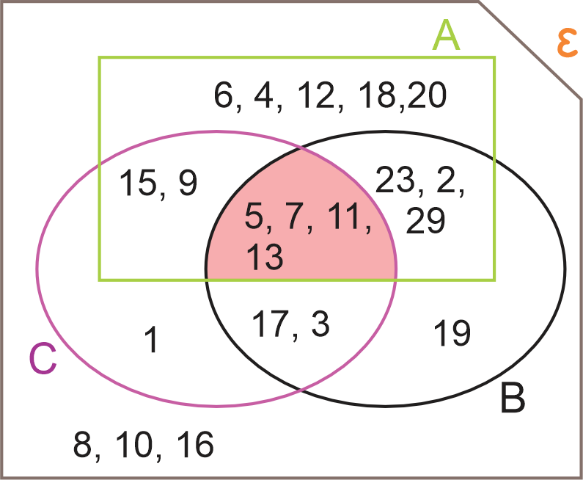
\includegraphics[width=0.55\textwidth]{figures/exercise-q1.png}
\end{center}

\begin{enumerate}
  \item[a.] List the elements in $A$, $B$ and $C$.
  \item[b.] List the elements in $A'$, $B'$ and $C'$.
  \item[c.] Find (i) $(A\cup B\cup C)'$ \quad (ii) $A'\cap B'\cap C'$ \quad (iii) $(A\cap B\cap C)'$ \quad (iv) $A'\cup B'\cup C'$.
  \item[d.] Compare your result in (c)(i) to (c)(ii). What conclusion can you draw?
  \item[e.] Compare your result in (c)(iii) to (c)(iv). What conclusion can you draw?
  \item[f.] Describe set $B$.
  \item[g.] Describe set $C$.
\end{enumerate}

\item Study the diagram carefully and use it to answer the questions.

\begin{center}
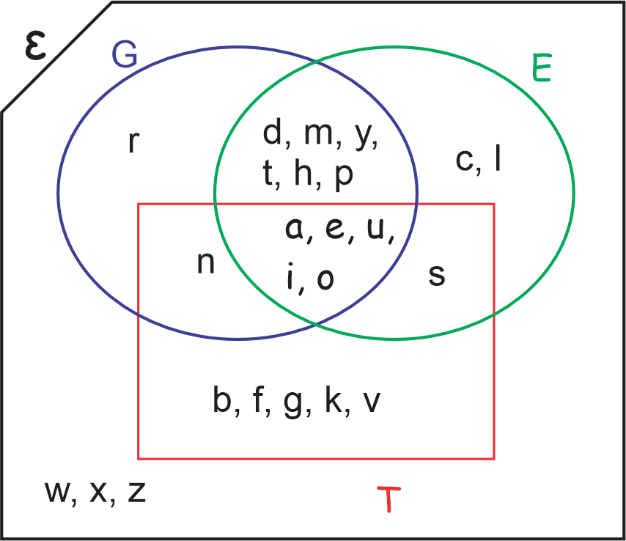
\includegraphics[width=0.55\textwidth]{figures/exercise-q2.png}
\end{center}

\begin{enumerate}
  \item[a.] List the elements in $G$, $E$, $T$ and $\varepsilon$.
  \item[b.] Show that $G' \cap E' = (G\cup E)'$.
  \item[c.] Show that $(G\cap E\cap T)' = G'\cup E'\cup T'$.
  \item[d.] Show that $(G\cup E\cup T)' = G'\cap E'\cap T'$.
\end{enumerate}

\end{enumerate}

\noindent For questions 3--7, sets $X$, $Y$ and $Z$ are subsets of the universal set $\mu$.
Use the information to choose the correct answer to the questions.

\begin{enumerate}[resume]
\item Find $X \cup X'$. \\
\textbf{A.} $\varnothing$ \quad \textbf{B.} $\mu$ \quad \textbf{C.} $X$ \quad \textbf{D.} $Y$

\item Find $Z \cap Z'$. \\
\textbf{A.} $\varnothing$ \quad \textbf{B.} $\mu$ \quad \textbf{C.} $Z$ \quad \textbf{D.} $X$

\item Find $(Y')'$. \\
\textbf{A.} $\varnothing$ \quad \textbf{B.} $\mu$ \quad \textbf{C.} $X$ \quad \textbf{D.} $Y$

\item Find $(X\cup X')'$. \\
\textbf{A.} $\varnothing$ \quad \textbf{B.} $\mu$ \quad \textbf{C.} $X$ \quad \textbf{D.} $X'\cup X$

\item Find $(Z\cap Z')'$. \\
\textbf{A.} $\varnothing$ \quad \textbf{B.} $\mu$ \quad \textbf{C.} $X\cup Y$ \quad \textbf{D.} $Z'\cap Z$

\item Rewrite:
\begin{enumerate}
  \item[a.] $(R\cup S')'$
  \item[b.] $(M'\cap N)'$
  \item[c.] $[(A'\cup B)'\cap C]'$
  \item[d.] $[(P\cap Q')'\cup P]'$
  \item[e.] $[A\cap(A'\cup B)']'$
\end{enumerate}

\item Show that
\begin{enumerate}
  \item[a.] $[(R\cup M)'\cap P]' = R\cup M\cup P'$
  \item[b.] $[(R\cap M)\cup M']' = R'\cap M$
\end{enumerate}

\item On a Venn diagram, shade the region represented by:
\begin{enumerate}
  \item[a.] $(A\cap B)'\cap C$
  \item[b.] $A'\cup(Y\cap Z')$
  \booknote[S1-05]{printed as in the book; the diagram's sets are $A$, $B$, $C$, so $Y$, $Z$
  are meant to be $B$, $C$.}
\end{enumerate}

\item Sets $X = \{\text{prime numbers}\}$, $Y = \{W : 0 < W \le 11\}$ and
$Z = \{1,2,3,4,5,6,7,13,14,15,16,18\}$ are subsets of $A = \{0,1,2,3,4,\ldots,21\}$.
\begin{enumerate}
  \item[a.] List the members of the following sets:
  \begin{enumerate}
    \item[i.] $X$
    \item[ii.] $Y$
    \item[iii.] $X\cap Y\cap Z$
    \item[iv.] $X\cup Y'$
    \item[v.] $(X\cup Y)\cap Z'$
    \item[vi.] $(X'\cap Y)\cup Z$
  \end{enumerate}
  \item[b.] Use a Venn diagram to represent $X$, $Y$, $Z$ and $A$.
\end{enumerate}

\item A survey of 90 teachers reveals the following. 45 teach Management, 57
Accounting and 50 Costing. 25 teach Management and Accounting, 35 teach
Accounting and Costing and 22 teach Management and Costing. 5 teachers
cannot teach any of the three subjects.
\begin{enumerate}
  \item[a.] Represent the information on a Venn diagram.
  \item[b.] Calculate the number of teachers who can teach only one of the three subjects.
\end{enumerate}

\item A survey of 41 employees shows that 25 are skilled in Carpentry, 15 in
Brick laying and 24 in Tiling. 12 are skilled in carpentry and brick laying,
9 in brick laying and tiling, 17 in carpentry and tiling, and 8 are not
skilled in any of the three occupations. Find the number of employees who
are skilled in
\begin{enumerate}
  \item[a.] all three occupations
  \item[b.] exactly two of the occupations
\end{enumerate}

\item A class of 60 students were each required to have textbooks in Accounting,
Management and Costing. However, when the class teacher checked their
books, she found out that: 16 had Accounting and Management books, 14
had Accounting and Costing books, 18 had only two of the three books and
20 had Accounting plus at least one other book. Every student had at
least one of the three books. Find the number of students who had
\begin{enumerate}
  \item[a.] all three books.
  \item[b.] only Costing and Accounting books.
  \item[c.] exactly one of the three books.
  \item[d.] If 16 students had neither Accounting nor Costing books, find the
  probability that a student selected at random from the class had Management books.
\end{enumerate}

\item The analysis of results of a sample of students who sat for the WASSCE
in Biology, Physics and Mathematics revealed that: 80\% passed in Biology,
65\% passed in Mathematics, 70\% passed in Physics, 52\% passed in Biology
and Mathematics, 58\% passed in Biology and Physics, 55\% passed in
Physics and Mathematics, 45\% passed in all three subjects. What
percentage of the students:
\begin{enumerate}
  \item[a.] passed only Mathematics
  \item[b.] passed only Physics
  \item[c.] passed only Biology
  \item[d.] passed Biology and Physics but not Mathematics
  \item[e.] did not pass any of the subjects.
\end{enumerate}

\item A shop owner kept records of purchases made by customers over the
weekend. The shop sells food, clothing and hardware. She found that, out
of the customers who visited her shop, 210 purchased food products, 100
hardware and 147 clothing. 30 purchased food and hardware. 128 purchased
two of the three products. She also found that of those who purchased two
of the three products, 14 did not buy clothing and 20 did not buy food. 13
of the customers who visited the store did not buy any of the products.
\begin{enumerate}
  \item[a.] How many customers visited the store over the weekend?
  \item[b.] How many of the customers who visited the store:
  \begin{enumerate}
    \item[i.] purchased less than two products.
    \item[ii.] purchased all three products.
    \item[iii.] purchased food and other products.
  \end{enumerate}
\end{enumerate}

\item A group of 210 tourists were asked to indicate which of the languages,
German, French and English they can speak. It was found that 55 can
speak German, 76 can speak French and 200 can speak English. 103 can
speak two of the three languages and 6 tourists cannot speak any of the
three languages. Find the number of tourists who can speak:
\begin{enumerate}
  \item[a.] all three languages
  \item[b.] only one of the three languages.
\end{enumerate}

\item 87 schools in Tamale have subscriptions to at least one of the following
newspapers: Graphic, Mirror and Times. 69 subscribe to Graphic, 62 to
Mirror and 55 to Times. 32 have subscriptions to all three newspapers.
Find the number of schools who have subscriptions to:
\begin{enumerate}
  \item[a.] exactly two of the newspapers
  \item[b.] only one of the newspapers.
\end{enumerate}

\item A publishing company surveyed its employees about their proficiency in
three software: Photoshop, CorelDraw and InDesign. The results show that
all the employees were proficient in at least one of the three software and
10 were proficient in all three. The number of employees proficient in
CorelDraw and other software were twice those proficient in only
CorelDraw. Of the employees who were proficient in two of the software,
14 were not proficient in InDesign, 8 were not proficient in CorelDraw and
6 were not proficient in Photoshop. The same number of employees
proficient in only InDesign are proficient in only Photoshop. There were
more employees proficient in only Photoshop and InDesign than employees
proficient in only Photoshop and there were fewer employees proficient in
only InDesign and CorelDraw than employees proficient in only InDesign.
\begin{enumerate}
  \item[a.] Use a Venn diagram to represent the above data.
  \item[b.] How many employees were involved in the survey?
  \item[c.] How many employees were proficient in only one of the software?
\end{enumerate}

\end{enumerate}

\subsection*{Part B}

\begin{enumerate}
\item Write down the first five terms of the binomial expansion of:
\begin{enumerate}
  \item[a.] $(1+4x)^{12}$
  \item[b.] $(1-3x)^9$
  \item[c.] $(3+2x)^7$
  \item[d.] $\left(1-\dfrac{x}{2}\right)^8$
  \item[e.] $\left(2-\dfrac{5}{2}x\right)^6$
\end{enumerate}

\item Write down the term indicated in the binomial expansion of the following
functions:
\begin{enumerate}
  \item[a.] $(1+3x)^6$: 3rd term
  \item[b.] $\left(1+\dfrac{x}{3}\right)^{20}$: 7th term
  \item[c.] $(a+4b)^{12}$: term containing $a^4$
\end{enumerate}

\item Expand the following binomial expansions up to and including the terms
in $x^2$:
\begin{enumerate}
  \item[a.] $(1-2x)(1+x)^8$
  \item[b.] $(2+3x)(1+3x)^{10}$
  \item[c.] $(5+2x)\left(1-\dfrac{2}{3}x\right)^{12}$
  \item[d.] $(1+4x)(1-3x)^{20}$
\end{enumerate}

\item Expand $(1-2x)^7$ and hence find the value of $(0.98)^7$ correct to 4 decimal
places.

\item Find the first four terms of the following using the binomial theorem.
\begin{enumerate}
  \item[a.] $\left(1-\dfrac{1}{2}x\right)^{1/2}$
  \item[b.] $(1-2x)^{-3}$
  \item[c.] $(3-x)^{-2}$
\end{enumerate}

\item Use appropriate binomial expansions to find the approximate values of:
\begin{enumerate}
  \item[a.] $\sqrt[3]{8.7}$ correct to 5 significant figures.
  \item[b.] $(81.162)^{1/4}$ to 4 decimal places.
  \item[c.] $\sqrt{4.02}$ to 3 decimal places.
  \item[d.] $\dfrac{1}{\sqrt{10}}$ to 4 decimal places.
  \item[e.] $\sqrt{101}$ to 4 decimal places.
  \item[f.] $(0.995)^5$ to 4 decimal places.
\end{enumerate}

\item Show that in ascending powers of $x$, $\left(\dfrac{1-x}{1+x}\right)^{1/3}$ is
$1 - \dfrac{2}{3}x + \dfrac{2}{9}x^2 - \dfrac{4}{21}x^3 - \cdots$.

\item Expand the following as far as the $x^3$ term:
\begin{enumerate}
  \item[a.] $(1+x+2x^2)^3$
  \item[b.] $(1+3x+x^2)^4$
\end{enumerate}

\item
\begin{enumerate}
  \item[a.] Find the first 3 terms in ascending powers of $x$ of the binomial
  expansion $(1+py)^9$, where $p$ is a non-zero constant.
  \item[b.] If the first 3 terms are $1$, $36x$ and $qx^2$ where $q$ is a constant, find
  the value of $p$ and $q$.
  \booknote[S1-06]{as printed: part (a) expands in $y$ and part (b) gives the terms in $x$.}
\end{enumerate}

\item
\begin{enumerate}
  \item[a.] Find the first 3 terms in ascending powers of $x$ of the binomial
  expansion $(2+kx)^7$, where $k$ is a constant.
  \item[b.] Given that the coefficient of $x^2$ is 6 times the coefficient of $x$, find
  the value of $k$.
\end{enumerate}

\end{enumerate}


\chapter{Sequences and Inequalities}
% Book p. 50 (PDF p. 51)
\section*{Modelling with Algebra}
\subsection*{Application of Algebra}

\subsubsection*{Introduction}

Studying sequences and inequalities is important because arithmetic and
geometric sequences provide statistical understanding into central tendencies,
growth rates, etc. Also, quadratic inequalities help in decision-making processes
where certain conditions or constraints must be met. For example, in business
and economics, they are used to model profit maximisation or loss minimisation
under specific constraints. In physics and engineering, quadratic inequalities arise
when determining safe operating conditions, or analysing forces. In architecture
and design, they help define areas, volumes or structural integrity within specific
boundaries. This section introduces you to the concept of the sum of sequences,
convergent and divergent series, recursive sequences, arithmetic and geometric
sequences. You will also learn how to solve quadratic inequalities, systems of
quadratic inequalities and real-life problems involving quadratic inequalities.

\begin{keyideas}
\begin{itemize}
  \item A \textbf{sequence} is a set of numbers in a given order.
  \item Each of the numbers in a sequence is called a term.
  \item Maximum values are the largest possible values of variables within a
  system that satisfy a set of constraints, each represented by an inequality.
  \item Minimum values are the least possible values of variables within a system
  that satisfy a set of constraints, each represented by an inequality.
  \item When finding the solution to a quadratic inequality, it is advisable to start
  by sketching the associated quadratic graph.
\end{itemize}
\end{keyideas}

% Book pp. 51-53 (PDF pp. 52-54)
\section{Sum of Sequences}

In year one we identified number patterns and classified them into arithmetic and
geometric sequences. While sequences are a list of numbers with defined patterns,
a series is the sum of the terms of a sequence. This year we will be finding the
sum of sequences and analysing the convergence or divergence of series.

If the general term of a series with $n$ term is known, then the complete series can
be written down in short notation as indicated by the following:
\begin{enumerate}
  \item $a + (a+d) + (a+2d) + \ldots + (a+[n-1]d) = \sum_{r=1}^{n} (a+[r-1]d)$
  \item $a + ar + ar^2 + \ldots ar^{n-1} = \sum_{k=1}^{n} ar^{k-1}$
  \item $1^2 + 2^2 + 3^2 + \ldots n^2 = \sum_{r=1}^{n} r^2$
  \item $-1^3 + 2^3 - 3^3 + 4^3 + \ldots (-1)^n n^3 = \sum_{r=1}^{n} (-1)^r r^3$
\end{enumerate}

\noindent\textbf{Notes:}
\begin{enumerate}
  \item[a.] It is sometimes more convenient to count the term of a series from zero
  rather than 1.

  For example:
  \[
    a + (a+d) + (a+2d) + \ldots + (a+[n-1]d) = \sum_{r=0}^{n-1} (a+rd) \text{ and}
  \]
  \[
    a + ar + ar^2 + \ldots ar^{n-1} = \sum_{k=0}^{n-1} ar^{k}
  \]
  In general, for a series with $n$ terms starting at $u_0$:
  \[
    u_0 + u_1 + u_2 + u_3 + \ldots u_{n-1} = \sum_{r=0}^{n-1} u_r
  \]
  \item[b.] We may also use the sigma notation for ``infinite series'' such as those already
  encountered in the sum to infinity of a geometric series.

  For example: $1 + \frac{1}{3} + \frac{1}{3^2} + \frac{1}{3^3} + \ldots = \sum_{r=1}^{\infty} \frac{1}{3^{r-1}}$
  or $\sum_{r=0}^{\infty} \frac{1}{3^{r}}$
\end{enumerate}

\begin{activity}{Activity 2.1 -- Sums of Sequences}
Perform this activity in pairs or groups.

In year one we learnt about Arithmetic and Geometric Progression. Let us
revise and build on that knowledge by creating the sequence terms and find
the sum of the terms of the expressions below.
\begin{enumerate}
  \item Evaluate $\sum_{n=0}^{6} 2(n-3)$
  \item Find the sum $\sum_{k=1}^{50} (3k+2)$
  \item Evaluate $\sum_{r=1}^{3} \left(\frac{1}{2}\right)^r$
\end{enumerate}

\solution
\begin{enumerate}
  \item $\sum_{n=0}^{6} 2(n-3) = 2(0-3) + 2(1-3) + 2(2-3) + 2(3-3) + 2(4-3) + 2(5-3) + 2(6-3)$
  \begin{align*}
    &= 2(-3) + 2(-2) + 2(-1) + 2(0) + 2(1) + 2(2) + 2(3) \\
    &= (-6) + (-4) + (-2) + 0 + 2 + 4 + 6 \\
    &= 0
  \end{align*}
  \item $\sum_{k=1}^{50} (3k+2)$
  \begin{align*}
    u_1 &= 3(1) + 2 = 5 \\
    u_{50} &= 3(50) + 2 = 152 \\
    s_k &= \frac{k\,(u_1 + u_{50})}{2} \\
    s_k &= \frac{50(5+152)}{2} = 3925
  \end{align*}
  \item $\sum_{r=1}^{3} \left(\frac{1}{2}\right)^r$
  \begin{align*}
    \text{when } r = 1,\ \left(\tfrac{1}{2}\right)^1 &= \tfrac{1}{2} \\
    \text{when } r = 2,\ \left(\tfrac{1}{2}\right)^2 &= \tfrac{1}{4} \\
    \text{when } r = 3,\ \left(\tfrac{1}{2}\right)^3 &= \tfrac{1}{8} \\
    \Longrightarrow \tfrac{1}{2} + \tfrac{1}{4} + \tfrac{1}{8} &= \tfrac{7}{8}
  \end{align*}
\end{enumerate}
\end{activity}

\subsection{Method of undetermined coefficients}

The method of undetermined coefficients is a powerful technique for finding the
general solution of linear recurrence relations with constant coefficients

If the $n$th term of a linear sequence is denoted by $x_n$, then the recurrence relation
is of the form: $x_{n+1} = f(x_n)$ for some of the function $f$.

For example, in $x_{n+1} = 4 - \frac{x_n}{2}$, when $x_2 = 2$, then $x_3$ is expressed as
$x_{2+1} = 4 - \frac{x_2}{2}$
\begin{align*}
  x_3 &= 4 - \frac{2}{2} \\
  x_3 &= 4 - 1 \\
  x_3 &= 3
\end{align*}

\begin{example}{Example 2.1}
The $n$th term of a sequence is $U_n$. If $U_1 = 3$ and $U_{n+1} = U_n + 5$, find $U_3$.

\solution
\begin{align*}
  U_{n+1} &= U_n + 5 \\
  U_1 &= 3 \\
  U_2 &= U_{1+1} = U_1 + 5, \text{ but } U_1 = 3 \\
  U_2 &= 3 + 5 = 8 \\
  U_3 &= U_{2+1} = U_2 + 5 \\
  U_3 &= 8 + 5 = 13
\end{align*}
\end{example}

% Book pp. 53-57 (PDF pp. 54-58)
\section{Sum of an Arithmetic Progression (AP)}

\begin{activity}{Activity 2.2}
\begin{enumerate}
  \item Working in pairs or small groups, work through the following steps to
  discover how to find the general sum of an arithmetic sequence, ie a
  sequence with a common difference.
  \item Let $Sn$ denote the sum of the first $n$ terms of a linear sequence, where
  ``$a$'' is the first term and ``$d$'' the common difference.
  \item $Sn = a + (a+d) + (a+2d) + \ldots + [a+(n-1)d] \ \ldots\ldots\ldots\ldots\ldots\ (1)$
  \item Writing the terms in the reverse order, we get :
  \item $Sn = [a+(n-1)d] + [a+2d(n-2)] + \ldots + (a+2d) + (a+d) + a \ \ldots\ldots\ldots\ (2)$

  Adding (1) and (2), we get
  \[
    2Sn = [2a+(n-1)d] + [2a+(n-1)d] + [2a+(n-1)] + \ldots = n[2a+(n-1)d]
  \]
  (Since we are adding $n$ terms we have $n$ lots of this expression.)
  \[
    \therefore Sn = \frac{n}{2}\big[2a + (n-1)d\big]
  \]
  \item Let $U_1 = a$,
  \item Then, $Sn = \frac{n}{2}\big[2U_1 + (n-1)d\big]$
  \item Similarly, $Sn = \frac{n}{2}\big[U_1 + \{U_1 + (n-1)d\}\big]$
  \item But $U_n = U_1 + (n-1)d$
  \item By substitution, we get
  \item $S_n = \frac{n}{2}\big[U_1 + U_n\big]$ (Remember that $U_1$ = the first term and $U_n$ = the last term)
\end{enumerate}
\booknote[S2-01]{the book prints the second term of line (2) as $[a+2d(n-2)]$ and the third bracket of
$2Sn$ as $[2a+(n-1)]$; the intended expressions are $[a+(n-2)d]$ and $[2a+(n-1)d]$.}
\end{activity}

\begin{example}{Example 2.2}
\begin{enumerate}
  \item[a.] Find the sum of the first 35 terms of the linear sequence 2, 5, 8\ldots
\end{enumerate}

\solution
\begin{align*}
  a &= 2,\ d = 3 \text{ and } n = 35 \\
  Sn &= \frac{n}{2}\big[2a + (n-1)d\big] \\
  S_{35} &= \frac{35}{2}\big[2(2) + (35-1)(3)\big] = 1855
\end{align*}

\begin{enumerate}
  \item[b.] A sequence is defined by $U_{n+1} = 3 + U_n$ and $U_1 = 1$
  \item[c.] Find the sum of the first ten term of the sequence.
\end{enumerate}

\solution
\begin{align*}
  U_{n+1} &= 3 + U_n \\
  U_1 &= 1\ (= a) \\
  U_2 &= 4
\end{align*}
Common difference $d = u_2 - u_1 = 4 - 1 = 3$
\[
  S_n = \frac{n}{2}[2a + (n-1)d],
\]
where $a$ = first term, $d$ the common difference and $n$ the number of terms
\begin{align*}
  S_{10} &= \frac{10}{2}[2(1) + (10-1)3] \\
  S_{10} &= 5[2 + 9(3)] \\
  S_{10} &= 5[29] \\
  S_{10} &= 145
\end{align*}

\begin{enumerate}
  \item[d.] Find the the sum of the first 10 positive even numbers:
\end{enumerate}

\solution
\begin{align*}
  S_{10} &= 2 + 4 + 6 + 8 + 10 \cdots + 18 + 20 \\
  S_n &= \frac{n}{2}[U_1 + U_n] = \frac{n}{2}[\textit{first term} + \textit{last term}] \\
  S_{10} &= \frac{10}{2}[2 + 20] = 5 \times 22 = 110
\end{align*}
\end{example}

\begin{example}{Example 2.3}
A conference hall has 189 seats, arranged in 9 rows. The organiser wants to
arrange the seats such that the difference in the number of seats between any two
consecutive rows is 5 seats. If there are 9 rows in total, how many seats should be
in the third row?

\solution
Number of rows $n = 9$

Capacity of the room $S_9 = 189$

Difference $d = 5$

Let the number of seats in the first row $= a$
\begin{align*}
  S_n &= \frac{n}{2}[2a + (n-1)d] \\
  S_9 &= \frac{9}{2}[2a + (9-1)5] \\
  189 &= \frac{9}{2}[2a + (8)5] \\
  378 &= 9[2a + (8)5] \\
  378 &= 18a + 360 \\
  18a &= 378 - 360 \\
  18a &= 18 \\
  a &= 1
\end{align*}
Number of seats in the third row $a + 2d \Rightarrow 1 + 2(5) = 11$
\end{example}

\subsection{Sum of a Geometric Progression (GP)}

Remember that a geometric progression has the first term, $a$ and a common ratio, $r$.

The position of terms represented by $n$ can be written as:
\begin{align*}
  S_n &= a + ar + ar^2 + ar^3 + \ldots + ar^{n-2} + ar^{n-1} \ \ldots\ldots\ (1) \\
  rS_n &= ar + ar^2 + ar^3 + \ldots\ldots + ar^{n-1} + ar^{n} \ \ldots\ldots\ (2)
\end{align*}
$\textit{eqn } (2) - \textit{eqn } (1)$
\begin{align*}
  rSn - Sn &= -a + ar^n \\
  S_n(r-1) &= ar^n - a \\
  S_n &= \frac{a(r^n - 1)}{r - 1} = \frac{-a(1 - r^n)}{-(1 - r)} \\
  S_n &= \frac{a(r^n - 1)}{r - 1},\ r \ne 1 \\
  S_n &= \frac{a(1 - r^n)}{(1 - r)},\ r \ne 1
\end{align*}

\begin{example}{Example 2.4}
Find the sum of the first seven terms of the sequence 2, 8, 32\ldots

\solution
\begin{align*}
  S_n &= \frac{a(r^n - 1)}{r - 1},\ r \ne 1 \\
  a &= 2,\ r = 4 \text{ and } n = 7 \\
  S_7 &= \frac{2(4^7 - 1)}{4 - 1} \\
  S_7 &= \frac{2(16384 - 1)}{3} \\
  S_7 &= \frac{2 \times 16\,382}{3} \\
  S_7 &= 10922
\end{align*}
\booknote[S2-02]{$4^7 - 1 = 16383$; the book's ``$16\,382$'' is a misprint, though the
final answer $10922$ is correct.}
\end{example}

\begin{example}{Example 2.5}
Find the sum of the first 10 terms of $\frac{1}{2}, \frac{1}{4}, \frac{1}{8}, \ldots$

\solution
\begin{align*}
  S_n &= \frac{a(1 - r^n)}{(1 - r)},\ r \ne 1 \\
  a &= \frac{1}{2},\ r = \frac{1}{2} \text{ and } n = 10 \\
  S_{10} &= \frac{\frac{1}{2}\left(1 - \left(\frac{1}{2}\right)^{10}\right)}{\left(1 - \frac{1}{2}\right)} \\
  S_{10} &= \frac{1}{2}\left(1 - \frac{1}{1024}\right) \\
  S_{10} &= \frac{1024 - 1}{1024} \\
  S_{10} &= \frac{1023}{1024}
\end{align*}
\booknote[S2-03]{the line $S_{10} = \frac{1}{2}\left(1 - \frac{1}{1024}\right)$ is printed as in the
book; dividing by $\left(1 - \frac{1}{2}\right)$ cancels the $\frac{1}{2}$, which is why the
next line is $\frac{1024-1}{1024}$.}
\end{example}

% Book pp. 57-58 (PDF pp. 58-59)
\section{Convergence and Divergence of Series}

A series is a sum of a sequence of numbers. For example, $1 + 2 + 3 + 4 + \ldots$

\subsection{Convergence of series}

A series is \textbf{convergent} if its sum approaches a finite value. Think of it like a target.
\begin{enumerate}
  \item The series get closer and closer to the target (the finite value).
  \item The sum of the series stabilises.
  \item Example, $1 + \frac{1}{2} + \frac{1}{4} + \frac{1}{8} + \ldots$
  \item As n increases the nth term is converging to 0 and the sum of the series is
  converging to 2.
  \item If the limit of the $n$th term is 0, the series might converge.
  \item If the ratio between the terms is constant, then the series converges when
  $|r| < 1$.
\end{enumerate}

\subsection{Divergence}

A series is \textbf{divergent} if its sum grows without bounds or approaches infinity.
Think of it like a runaway train:
\begin{enumerate}
  \item The series gets farther and farther away from a finite value.
  \item The sum of the series increases indefinitely.
  \item Example; $1 + 2 + 4 + 8 + \ldots$ this series diverges.
\end{enumerate}
If the limit of the $n$th term is not 0, the series diverges.

If the ratio between term is greater than 1, the series diverges, ie $|r| > 1$

\subsection{Sum to infinity of a convergent Geometric Progression}

For the general exponential sequence (GP):

$S_n = \frac{a(1 - r^n)}{(1 - r)}$, \textit{if} $-1 < r < 1$, then $r^n$ becomes smaller and
smaller as $n$ becomes larger and larger, so as $n \longrightarrow \infty$ then $r^n \to 0$
and $(1 - r^n) \to 1$.

We say the limiting value is denoted $S_\infty$ is $\frac{a}{1 - r}$.

Hence, the sum to infinity of $a, ar, ar^2, \ldots$ is given by $S_\infty = \frac{a}{1 - r}$,
provided $-1 < r < 1$.

\begin{example}{Example 2.6}
Determine the sum to infinity of the geometric series $5, -1 + \frac{1}{5}, \ldots$

\solution
$5, -1 + \frac{1}{5}, \ldots$

$a = 5$, $r = -\frac{1}{5}$

The sum to infinity is
\begin{align*}
  S\infty &= \frac{a}{1 - r} \\
  &= \frac{5}{1 - \left(-\frac{1}{5}\right)} = \frac{5}{\left(\frac{6}{5}\right)}
     = \frac{25}{6} = 5\frac{1}{6}
\end{align*}
\booknote[S2-04]{the series is printed as ``$5, -1 + \frac{1}{5}, \ldots$'' in the book; the
intended geometric series is $5, -1, \frac{1}{5}, \ldots$}
\end{example}

\noindent\textbf{Note:} $S_1, S_2, S_3, \ldots$ are the partial sums of the series. If there is
a number $L$ such that: $S_n = \sum_{r=1}^{\infty} Sn = L$. The number $L$ is called the
sum of the infinity series. If there is no such number, the series is said to diverge.

% Book pp. 58-62 (PDF pp. 59-63)
\section{Recursive Sequences}

A recursive sequence is a sequence where each term is defined using previous
terms.

For example, for an Arithmetic Sequence:

First term $a_1 = 2$

Recursive formula: $a_n = a_{n-1} + 3$
\begin{enumerate}
  \item Start with $a_1 = 2$
  \item To find $a_2$, add 3 to $a_1$ : $a_2 = 2 + 3 = 5$
  \item To find $a_3$, add 3 to $a_2$ : $a_3 = 5 + 3 = 8$
  \item To find $a_4$, add 3 to $a_3$ : $a_4 = 8 + 3 = 11$

  Sequence: 2, 5, 8, 11, 14, 17\ldots
\end{enumerate}

For example, for a Geometric Sequence:

First Term: $a_1 = 2$

Recursive formula: $a_n = 2 \times a_{n-1}$
\begin{enumerate}
  \item Start with $a_1 = 2$
  \item To find $a_2$, multiply $a_1$ \textit{by} $2 \to a_2 = 2 \times 2 = 4$
  \item To find $a_3$, multiply $a_2$ \textit{by} $2 \to a_3 = 2 \times 4 = 8$
  \item To find $a_4$, multiply $a_3$ \textit{by} $2 \to a_4 = 2 \times 8 = 16$

  Sequence: 2, 4, 8, 16, 32, 64, \ldots
\end{enumerate}

In both examples;
\begin{itemize}
  \item The first term $(a_1)$ is given
  \item The recursive formula defines how to find the next term $(a_n)$ using the
  previous term $(a_{n-1})$
\end{itemize}

\subsection{Recurrent decimals}

Recurrent decimals are repeated decimals. It can be seen that every recurrent
decimal represents a rational number. Every rational number can be represented
by a terminal decimal or a recurrent decimal. If the denominator of a rational
number (written in its simplest form) has prime factors, other than 2 and 5, then
the rational number is recognised as a recurrent decimal.

For example; $\frac{5}{9} = 0.5555\ldots$ \textit{or} $0.\dot{5}$,
$\frac{2}{11} = 0.181818\ldots$ \textit{or} $0.\dot{1}\dot{8}$,
$\frac{8}{15} = 0.53333\ldots$ \textit{or} $0.5\dot{3}$

\begin{example}{Example 2.7}
Write the recurring decimals as a series. Identify the common ratio, the first term
and an explicit formula for the $n$th term:
\begin{enumerate}
  \item[a.] 0.222222\ldots
  \item[b.] 0.323232\ldots
  \item[c.] 5.414141\ldots
\end{enumerate}

\solution
\begin{enumerate}
  \item[a.] $0.2222... = 0.2 + 0.02 + 0.002 + 0.0002 + \cdots$
  \begin{align*}
    &= 0.2 + 0.2(0.1) + 0.2(0.01) + 0.2(0.001) + \cdots \\
    &= 0.2 + 0.2(0.1) + 0.2(0.1)^2 + 0.2(0.1)^3 + \cdots
  \end{align*}
  The first term is 0.2, and the common ratio between each successive term is
  0.1. The formula for the $n$th term will be $U_n = 0.2\left(\frac{1}{10}\right)^{n-1}$

  \item[b.] $0.323232\ldots = 0.32 + 0.0032 + 0.000032 + 0.00000032 + \cdots$
  \begin{align*}
    &= 0.32 + 0.32(0.01) + 0.32(0.0001) + 0.32(0.000001) + \cdots \\
    &= 0.32 + 0.32(0.01) + 0.32(0.01)^2 + 0.32(0.01)^3 + \cdots
  \end{align*}
  The first term is 0.32, and the common ratio between each successive term
  is 0.01. The formula for the $n$th term will be $U_n = 0.32\left(\frac{1}{100}\right)^{n-1}$

  \item[c.] $5.414141\ldots = 5 + 0.41 + 0.0041 + 0.000041 + 0.00000041 + \cdots$
  \[
    = 5 + 0.41 + 0.41(0.01) + 0.41(0.1)^2 + 0.41(0.1)^3 + \cdots
  \]
  From the second term (0.41), a geometric sequence with first term 0.41, and
  the common ratio 0.01 can be observed. The formula for the $n$th term will
  be

  For 0.414141\ldots, $U_n = 0.41\left(\frac{1}{100}\right)^{n-1}$

  Thus, $5.414141\ldots = 5 + 0.41\left(\frac{1}{100}\right)^{n-1}$ for $n = 1, 2, 3, \ldots$
  \booknote[S2-05]{the book prints $0.41(0.1)^2 + 0.41(0.1)^3$; with common ratio $0.01$ these
  should read $0.41(0.01)^2 + 0.41(0.01)^3$.}
\end{enumerate}
\end{example}

\begin{example}{Example 2.8}
Write 0.9999\ldots as an exponential series and show that in the limit, the sum of
series equals one.

\solution
$0.9999\ldots = 0.9 + 0.09 + 0.009 + 0.0009 + \ldots$

This is a G.P. with first term, $a = 0.9$ and common ratio, $r = \frac{0.09}{0.9} = 0.1$

The series is an infinite series with sum; $S_\infty = \frac{a}{1 - r} = \frac{0.9}{1 - 0.1}
= \frac{0.9}{0.1} = 1$
\booknote[S2-06]{$1 - 0.1 = 0.9$, so the last step should read $\frac{0.9}{0.9} = 1$; the book
prints $\frac{0.9}{0.1}$.}
\end{example}

\begin{example}{Example 2.9}
Express $0.1\dot{6}$ as an infinite geometric series and find the sum of the geometric
series.

\solution
\begin{align*}
  0.1\dot{6} &= 0.166666\ldots \\
  &= 0.1 + 0.06 + 0.006 + 0.0006 + \ldots \\
  &= \frac{1}{10} + \frac{6}{100} + \frac{6}{1000} + \frac{6}{10000} + \ldots
\end{align*}
From the series, the term after $\frac{1}{10}$ from geometric series with $= \frac{6}{100}$,
$r = \frac{6}{100} \div \frac{6}{1000} = \frac{1}{10}$

Sum of the geometric series:
\begin{align*}
  0.0\dot{6} = S_\infty &= \frac{\frac{6}{100}}{1 - \frac{1}{10}} \\
  &= \frac{\frac{6}{100}}{\frac{9}{10}} \\
  &= \frac{1}{15}
\end{align*}
$\therefore 0.1\dot{6} = \frac{1}{10} + \frac{1}{15} = \frac{1}{6}$
\booknote[S2-07]{the common ratio is $\frac{6}{1000} \div \frac{6}{100} = \frac{1}{10}$; the book
prints the division the other way round.}
\end{example}

\begin{example}{Example 2.10}
If a sequence $U_1, U_2, U_3\ldots$ is define by the relation $U_{n+1} = 3 + U_n$ for
$n \ge 1$ and $U_1 = 1$, find;
\begin{enumerate}
  \item[a.] $U_2, U_3$ and $U_4$
  \item[b.] a formula for $U_n$ in terms of $n$.
  \item[c.] the sum of the 1\textit{st} $n$ terms
\end{enumerate}

\solution
\begin{enumerate}
  \item[a.] Using the relation
  \begin{align*}
    U_{n+1} &= 3 + U_n \\
    \text{If } n &= 1 \\
    U_2 &= 3 + U_1 = 3 + 1 = 4 \\
    U_3 &= 3 + U_2 = 3 + 4 = 7 \\
    U_4 &= 3 + U_3 = 3 + 7 = 10
  \end{align*}
  The sequence is $1, 4, 7, 10, \ldots$, so it is a linear sequence
  \item[b.] $U_n = a + (n-1)d$ and $a = 1, d = 3$
  \begin{align*}
    U_n &= 1 + (n-1)3 \\
    U_n &= 1 + 3n - 3 \\
    U_n &= 3n - 2
  \end{align*}
  \item[c.] The sum of $n$ terms of $1, 4, 7, 10, \ldots$
  \begin{align*}
    S_n &= \frac{n}{2}[2a + (n-1)d] \\
    S_n &= \frac{n}{2}[2(1) + (n-1)3] \\
    S_n &= \frac{n}{2}[2 + 3n - 3] \\
    S_n &= \frac{n}{2}[3n - 1]
  \end{align*}
\end{enumerate}
\end{example}

% Book pp. 62-63 (PDF pp. 63-64)
\section{Arithmetic and Geometric Means of Sequences}

The mean of any two numbers, for example, a and b, is obtained by finding a half
of the sum of the numbers thus: \textit{Mean}, $(\mu) = \frac{1}{2}(a + b)$. The difference
between a and $\mu$ is equal to the difference, or distance, between $\mu$ and b i.e.,
$\mu - a = b - \mu$.

Now, $a$, $\mu$, $b$ form an arithmetic sequence since there is a common difference and
that for any arithmetic sequence with a and b as terms, some means namely,
$\mu_1, \mu_2, \mu_3, \ldots \mu_k$ can be found between a and b such that a,
$\mu_1, \mu_2, \mu_3, \ldots \mu_k$, b, remains an arithmetic sequence as
$\mu_1 - a = \mu_2 - \mu_1 = \ldots \mu_k - b$ and the means are equally spaced.

\begin{example}{Example 2.11}
\begin{enumerate}
  \item Find the arithmetic mean sequence of students' scores in mathematics test:
  80, 75, 90, 85, 95.
  \item A baker wants to increase the amount of sugar in a recipe from 200g to
  500g in four equal steps. What arithmetic sequence represents the amount
  of sugar (in grammes) added and what are the intermediate values?
\end{enumerate}

\solution
\begin{enumerate}
  \item Arithmetic mean $= \dfrac{80 + 75 + 90 + 85 + 95}{5} = \dfrac{425}{5} = 85$
  \item The baker wants to increase the sugar from 200g to 500g
  \begin{align*}
    500 - 200 &= 300g \\
    d &= \frac{300}{4 - 1} \\
    &= \frac{300}{3} \\
    &= 100g
  \end{align*}
  Arithmetic mean
  \begin{align*}
    200 + 100 &= 300g \\
    300 + 100 &= 400g \\
    400 + 100 &= 500g
  \end{align*}
  The arithmetic sequence: 200, 300, 400, 500.

  The intermediate sequence 300 \textit{and} 400.
\end{enumerate}
\end{example}

\subsection{Geometric mean}

The geometric mean of a sequence is the measure of the central tendency of the
sequence, similar to the arithmetic mean. However, it is calculated differently.

For a sequence of $n$ numbers $(a_1 \times a_2 \times a_3 \ldots a_n)^{\frac{1}{n}}$

\begin{example}{Example 2.12}
\begin{enumerate}
  \item Find the geometric mean of the sequence 2, 4, 8, 16
  \item Find the geometric mean of the sequence 10, 20, 40.
\end{enumerate}

\solution
\begin{enumerate}
  \item 2, 4, 8, 16
  \[
    (a_1 \times a_2 \times a_3 \ldots a_n)^{\frac{1}{n}}
  \]
  \[
    (2 \times 4 \times 8 \times 16)^{\frac{1}{4}} = \sqrt[4]{1024} = 5.65685\ldots \approx 5.7
  \]
  \item $(10 \times 20 \times 40)^{\frac{1}{3}} = \sqrt[3]{8000} = 20$
\end{enumerate}
\end{example}

% Book pp. 63-67 (PDF pp. 64-68)
\section{Determining Maximum/Minimum Values}

In year one, we learnt how to solve linear equations and inequalities using graphing
and algebraic reasoning. With this knowledge, we will be able to graph polygons
when given specific linear equations or inequalities which will help us determine
the maximum/minimum value for a function.

Working in pairs or groups, go through this activity to review graphing of linear
inequalities.

\begin{activity}{Activity 2.3 -- Graphing Linear Inequalities}
\begin{enumerate}
  \item Pick a graph book/sheet
  \item Represent the following inequalities graphically
  \begin{enumerate}
    \item[a.] $y \le 0.67x + 2$
    \item[b.] $y \le -x + 2$
    \item[c.] $y \ge -2$
  \end{enumerate}
  \item Write out the coordinates for the points at which the inequalities intersect.
  \item What polygon did the intersecting lines create?
  \item Does your graph look like the one in Figure. 2.1: Graphing Linear
  Inequalities?
\end{enumerate}
\begin{center}
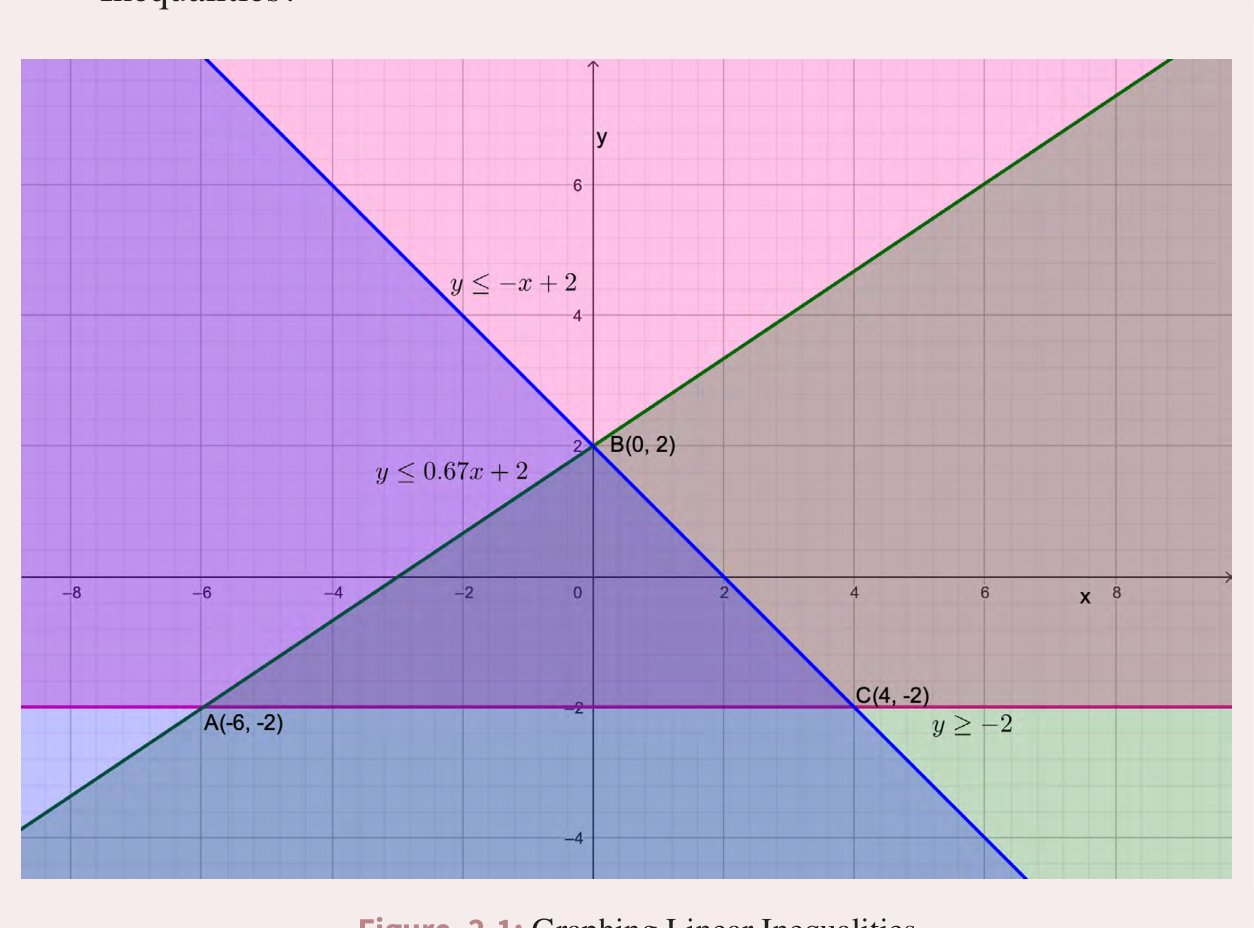
\includegraphics[width=0.85\linewidth]{figures/fig2-1.jpg}
\end{center}
\figcaption{2.1}{Graphing Linear Inequalities}
\end{activity}

Congratulations! You have adequately remembered how to graph linear
inequalities.

Now, we will learn how to determine the maximum/minimum value(s) of a given
function.

We can determine the maximum or minimum value of a given function based
on a specific objective. Maximum values are the highest points of a function
while minimum values are the lowest points of a function. In finding maximum
or minimum values of a function algebraically, you have to substitute all the
coordinates of the vertices of the region of interest that forms the solution to the
function. For example, if you are interested in getting the maximum/minimum
area of a given rectangle, you would evaluate the function at each corner or
edge by substituting the coordinates. If the polygon of interest (triangle, square,
etc.) is represented graphically, you need to identify the pair of coordinates and
substitute in the given function. On the other hand, if equations of lines are given,
you solve these equations simultaneously and determine the values for the pair of
coordinates.

\begin{example}{Example 2.13}
Evaluate the expression $V = 2x - 3y$ for the given feasible region to determine
the point at which `V' has a maximum value and the point at which `V' has a
minimum value.
\begin{center}
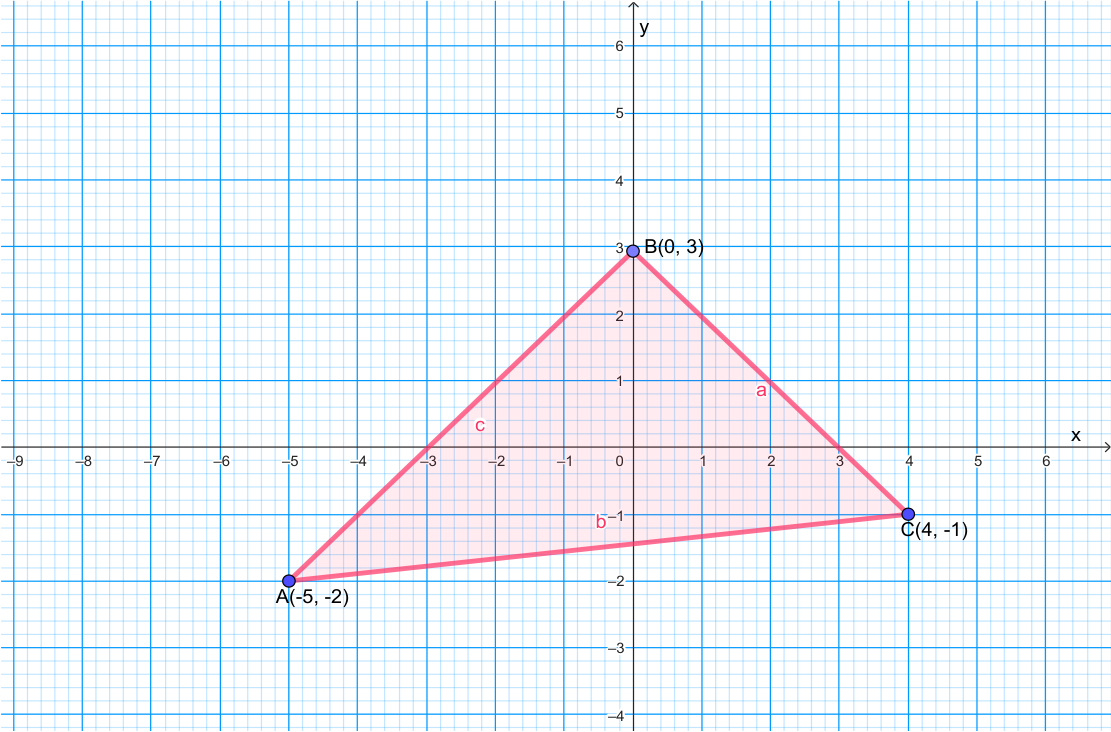
\includegraphics[width=0.8\linewidth]{figures/fig2-2.png}
\end{center}
% The book prints this graph without a caption; the solution calls it Figure 2.2.

\solution
\textbf{Step 1:} Identify all the vertices in Figure. 2.2

A $(-5, -2)$, B$(0, 3)$ and C $(4, -1)$

\textbf{Step 2:} Substitute the coordinates of each of the vertices in the function
$V = 2x - 3y$ and compute.

For $(-5, -2)$, $x = -5$, $y = -2$.
\begin{align*}
  V &= 2(-5) - 3(-2) \\
    &= -4
\end{align*}
For $(0, 3)$, $x = 0$, $y = 3$.
\begin{align*}
  V &= 2(0) - 3(3) \\
    &= -9
\end{align*}
For $(4, -1)$, $x = 4$, $y = -1$.
\begin{align*}
  V &= 2(4) - 3(-1) \\
    &= 11
\end{align*}

\textbf{Step 3:} Choose the highest result as the maximum value and the least as the
minimum value

Maximum value is 11 at vertex $(4, -1)$.

Minimum value is $-9$ at vertex $(0, 3)$.
\end{example}

\begin{example}{Example 2.14}
On the same graph, illustrate the inequalities, $y \ge \frac{7}{3}x - 5$, $y \le x - 1$ and
$x \ge 0$.

Using the polygon created, determine the minimum and maximum values of the
function $m = 7x - y$.

\solution
\textbf{Step 1:} Draw the three linear inequalities on a graph sheet.
\begin{center}
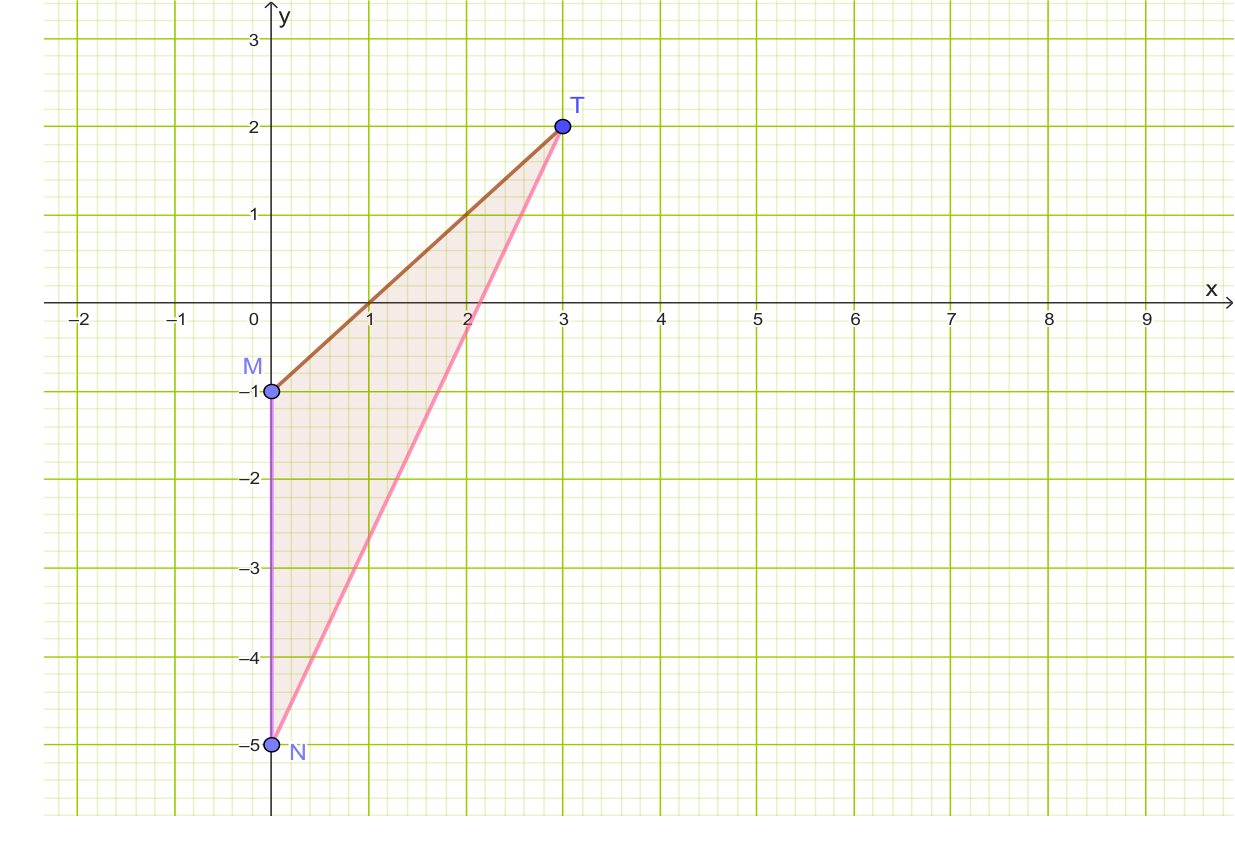
\includegraphics[width=0.85\linewidth]{figures/fig2-3.png}
\end{center}
\figcaption{2.3}{Graphical representation of inequalities in Example 2.14}

\textbf{Step 2:} Identify the coordinates of the vertices polygon created as a result of the
intersection of the lines.

M$(0, -1)$, T$(3, 2)$ and N$(0, -5)$

\textbf{Step 3:} Substitute the values of the coordinates in the function $m = 7x - y$.

For $(0, -1)$, $x = 0$, $y = -1$.
\begin{align*}
  m &= 7(0) - (-1) \\
    &= 1
\end{align*}
For $(3, 2)$, $x = 3$, $y = 2$.
\begin{align*}
  m &= 7(3) - 2 \\
    &= 19
\end{align*}
For $(0, -5)$, $x = 0$, $y = -5$.
\begin{align*}
  m &= 7(0) - (-5) \\
    &= 5
\end{align*}

\textbf{Step 4:} Select the highest result as the maximum value and the least as the
minimum value

Maximum value is 19 at vertex $(3, 2)$.

Minimum value is 1 at vertex $(0, -1)$.
\end{example}

\begin{example}{Example 2.15}
On the same graph, illustrate the inequalities, $x + y \le 8$, $y \ge 2$, $x - y \le 3$,
$-x + 2y \le 10$ and $x \ge 1$. Using the boundaries of the polygon created, determine the
minimum and maximum values of the function $w = x^2 + y^2$.

\solution
Step 1: Draw the five linear inequalities on a graph sheet.
\begin{center}
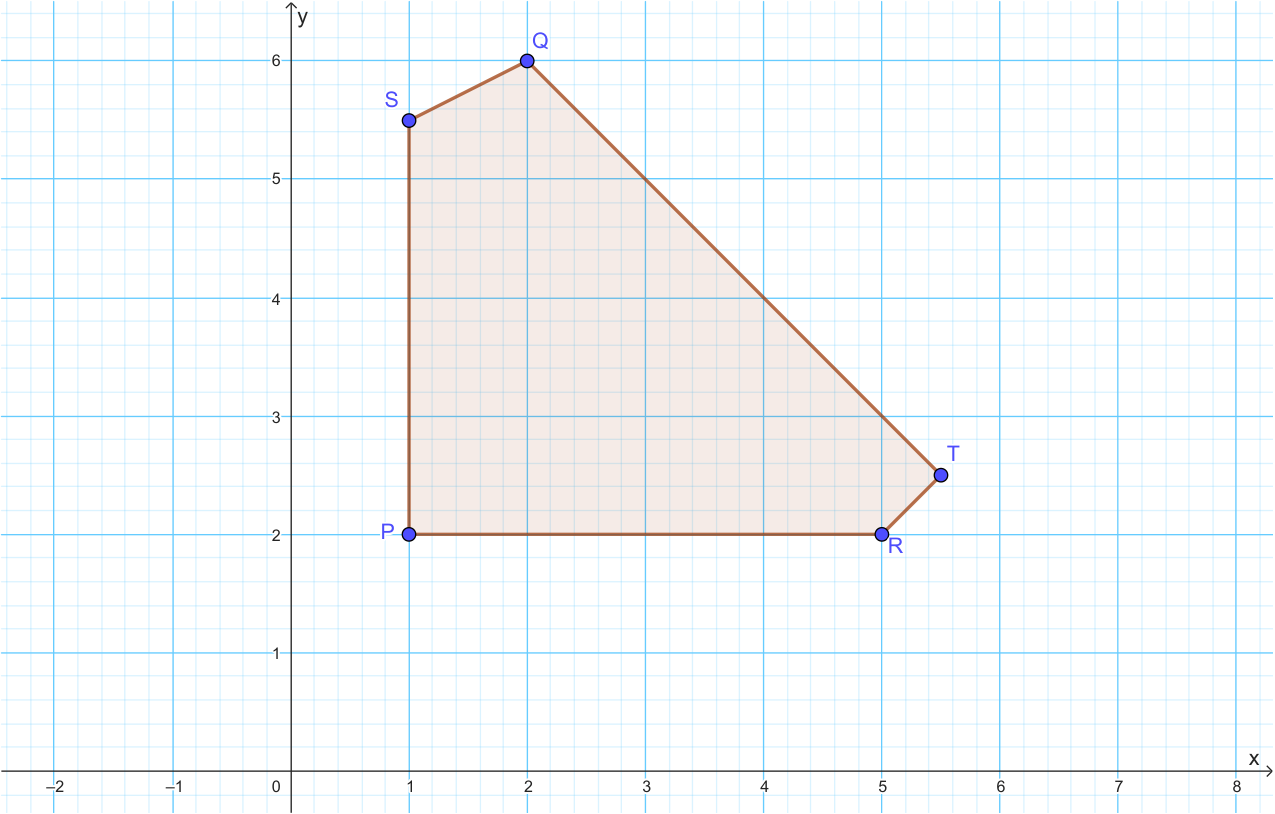
\includegraphics[width=0.85\linewidth]{figures/fig2-4.png}
\end{center}
\figcaption{2.4}{Graphical representation of inequalities in Example 2.15}

\textbf{Step 2:} Identify the coordinates of the vertices polygon created as a result of the
intersection of the lines.

P$(1, 2)$, S$(1, 5.5)$, Q$(2, 6)$, T$(5.5, 2.5)$ and R$(5, 2)$

\textbf{Step 3:} Substitute the values of the coordinates in the function $w = x^2 + y^2$.

For $(1, 2)$, $x = 1$, $y = 2$.
\begin{align*}
  w &= (1)^2 + (2)^2 \\
    &= 5
\end{align*}
For $(1, 5.5)$, $x = 1$, $y = 5.5$.
\begin{align*}
  w &= (1)^2 + (5.5)^2 \\
    &= 31.25
\end{align*}
For $(2, 6)$, $x = 2$, $y = 6$.
\begin{align*}
  m &= (2)^2 + (6)^2 \\
    &= 40
\end{align*}
For $(5.5, 2,5)$, $x = 5.5$, $y = 2.5$.
\begin{align*}
  m &= (5.5)^2 + (2.5)^2 \\
    &= 36.5
\end{align*}
For $(5, 2)$, $x = 5$, $y = 2$.
\begin{align*}
  m &= (5)^2 + (2)^2 \\
    &= 29
\end{align*}

\textbf{Step 4:} Select the highest result as the maximum value and the least as the
minimum value

Maximum value is 40 at vertex $(2, 6)$.

Minimum value is 5 at vertex $(1, 2)$.
\booknote[S2-08]{the last three substitutions are printed with ``$m =$'' in the book although
the function is $w$; ``$(5.5, 2,5)$'' is also as printed.}
\end{example}

Now, let's see how our knowledge on solving linear inequalities can be used to
solve real life problems.

% Book pp. 68-73 (PDF pp. 69-74)
\section{Solving Real Life Problems Involving Systems of Linear Inequalities}

Knowledge for knowledge's sake is commendable. However, utility of the
knowledge is even more satisfying. Let us go through this activity to explore the
usefulness of knowledge on solving systems of linear equations.

\begin{activity}{Activity 2.4 -- Optimising the Production of Furniture}
Working in pairs, or small groups, work on this activity.

\textbf{Scenario}

Kpogas company manufactures two types of products (chairs and tables).

Each chair requires 2 hours of carpentry and 1 hour of painting, while each
table requires 3 hours of carpentry and 2 hours of painting. The company has
a maximum of 60 hours of carpentry and 40 hours of painting available per
week.

They make a profit of \cedi50.00 per chair and \cedi80.00 per table.

How many chairs (c) and tables (t) should be produced each week to maximise
profit, while staying within the carpentry and painting constraints?

\solution
\begin{enumerate}
  \item Write out algebraic expressions for the hours of carpentry and painting.

  Hours for carpentry: $2c + 3t \le 60$

  Hours for painting: $c + 2t \le 40$
  \item Write out algebraic expressions for the number of chairs and tables.

  Number of chairs cannot be negative: c $\ge 0$

  Number of tables cannot be negative: t $\ge 0$
  \item Write out an equation for the expected profit.

  Let P represent profit

  P = 50c + 80t
  \item Express the system of linear inequalities as the constraints of production.
  \[
    \begin{cases}
      c \ge 0 \\
      t \ge 0 \\
      2c + 3t \le 60 \\
      c + 2t \le 40
    \end{cases}
  \]
  \item Note that the equation of profit is the objective function.
  \item Graph the system of linear inequalities
  \begin{center}
  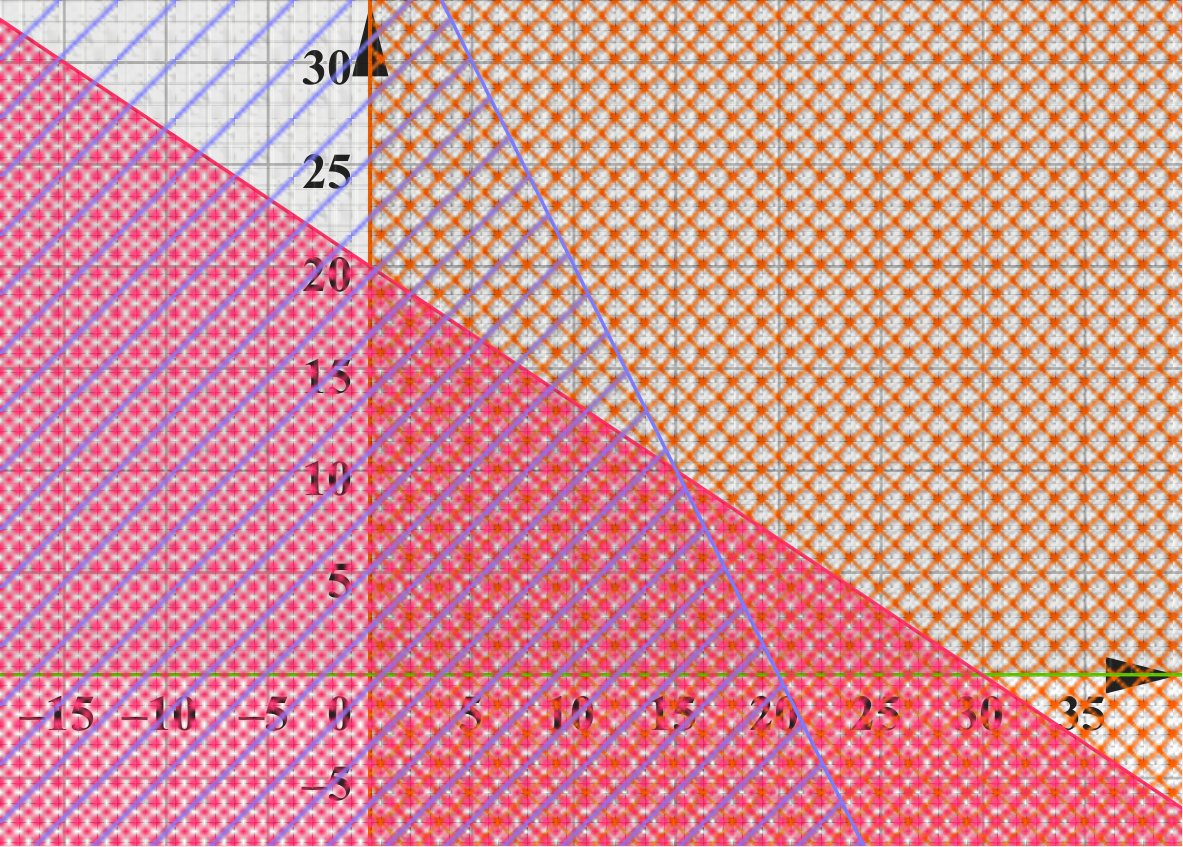
\includegraphics[width=0.85\linewidth]{figures/fig2-5.jpg}
  \end{center}
  \figcaption{2.5}{Graphical representation of Kpogas company production constraints}
  \item Identify the coordinates of the vertices to the solution region.

  $(20, 0)$, $(0, 0)$, $(15, 10)$ and $(0, 20)$
  \item Substitute the coordinates of the vertices into the profit equation.
  \begin{align*}
    \text{At } (20, 0),\ \text{P} &= 50(20) + 80(0) \\
      &= 1000 \\
    \text{At } (0, 0),\ \text{P} &= 50(0) + 80(0) \\
      &= 0 \\
    \text{At } (15, 10),\ \text{P} &= 50(15) + 80(10) \\
      &= 1550 \\
    \text{At } (0, 20),\ \text{P} &= 50(0) + 80(20) \\
      &= 1600
  \end{align*}
  \item Write out your conclusion

  The maximum profit is \cedi1600.00, and it occurs when Kpogas
  produces no chairs and 20 tables.
\end{enumerate}
\end{activity}

\begin{example}{Example 2.16}
A bakery produces cakes ($x$) and cookies ($y$) daily. A cake takes 2 hours to make
while a batch of cookies takes 1 hour to make. The bakery can spend at most 12
hours per day baking. Each cake requires 3 units of flour and a batch of cookies
requires 1 unit of flour. The bakery has at most 15 units of flour available each
day. The bakery earns \cedi5.00 profit per cake and \cedi3.00 profit per batch of
cookies. Without an increase in the units of flour and hours of baking, how many
of each product should be baked daily to make the most profit?

\solution
\textbf{Step 1:} Identify the constraints communicated by the bakery.
\[
  \begin{cases}
    2x + y \le 12 \\
    3x + y \le 15 \\
    x \ge 0 \\
    y \ge 0
  \end{cases}
\]
\textbf{Step 2:} Write out the equation of the profit (objective function).

$P = 5x + 3y$

\textbf{Step 3:} Graph the inequalities.
\begin{center}
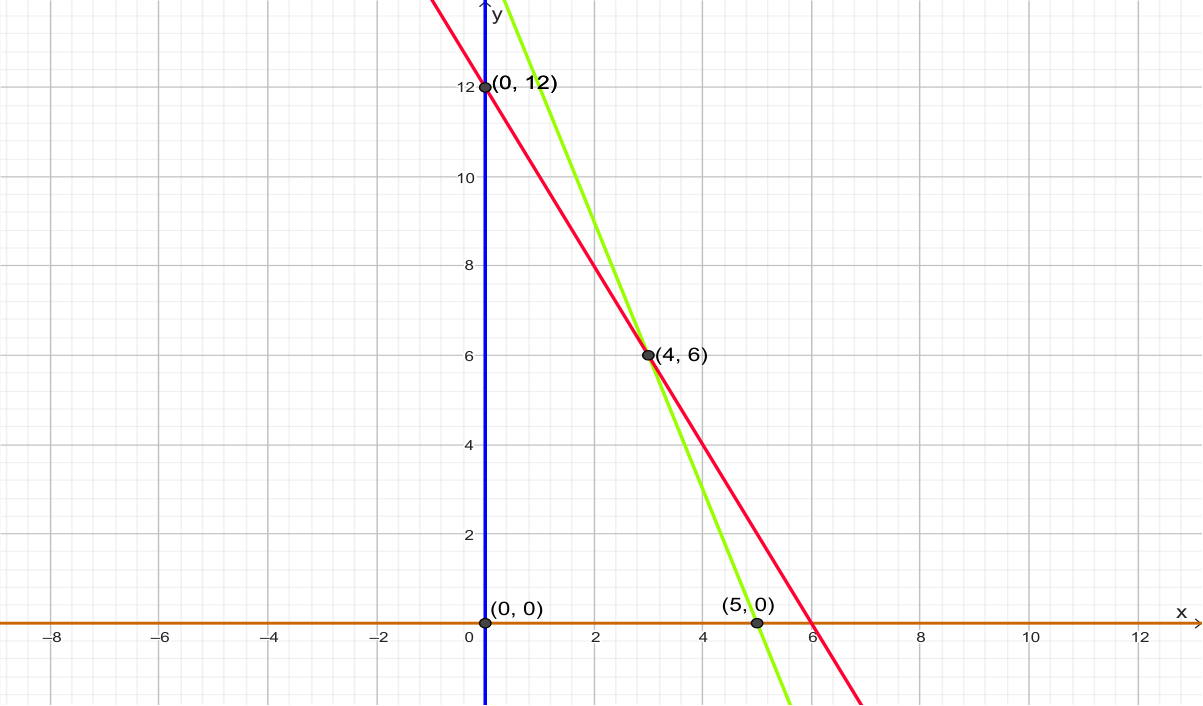
\includegraphics[width=0.85\linewidth]{figures/fig2-6.png}
\end{center}
\figcaption{2.6}{Graphical representation of constraints for baking}

\textbf{Step 4:} Identify the coordinates of the vertices to the solution region.

$(0, 12)$, $(5, 0)$, $(4, 6)$ and $(0,0)$

\textbf{Step 5:} Substitute the coordinates of the vertices into the profit equation.
\begin{align*}
  \text{At } (0, 12),\ \text{P} &= 5(0) + 3(12) \\
    &= 36 \\
  \text{At } (5, 0),\ \text{P} &= 5(5) + 3(0) \\
    &= 25 \\
  \text{At } (4, 6),\ \text{P} &= 5(4) + 3(6) \\
    &= 38 \\
  \text{At } (0, 0),\ \text{P} &= 5(0) + 3(0) \\
    &= 0
\end{align*}
\textbf{Step 6:} Write out your conclusion.

The bakery should bake 4 cakes and 6 batches of cookies daily to make the most
profit.
\end{example}

\begin{example}{Example 2.17}
A farmer has 300 metres of fencing material to enclose a rectangular field for
planting crops. The farmer wants to maximise the area of the field to get the best
crop yield, but there is a restriction. The length of the field must be 10 metres
longer than the width to accommodate the farm machinery.

What should be the dimensions of the field that will maximise the enclosed area,
keeping in mind the restriction on the total fencing available?

\solution
\textbf{Step 1:} Represent the statement algebraically.

Let w be the width of the field

Length of the field $=$ w $+\ 10$

\textbf{Step 2:} Write the equation for perimeter of the field.

Since Perimeter(P)$=$ 2(width) $+$ 2(length),
\begin{align*}
  \text{P} &= 2\text{w} + 2(\text{w} + 10) \\
  \text{P} &= 2\text{w} + 2\text{w} + 20 \\
  \text{P} &= 4\text{w} + 20.
\end{align*}
\textbf{Step 3:} Set up the linear inequality

Since the material available for fencing is 300m, the total distance around the
field can be less or equal to 300.

$4\text{w} + 20 \le 300$

\textbf{Step 4:} Simplify the inequality.
\begin{align*}
  4\text{w} &\le 300 - 20 \\
  4\text{w} &\le 280 \\
  \text{w} &\le \frac{280}{4} \\
  \text{w} &\le 70
\end{align*}
So, the width of the field must be less than or equal to 70 metres.

\textbf{Step 5:} Test values for width.

Since the highest value for the width will be 70, the length will be $70 + 10 = 80$

Testing for perimeter, $2(70) + 2(80) = 300$, satisfying perimeter requirement.

Testing for maximum area of the rectangular field: length $\times$ width

Area $= 70 \times 80 = 5600m^2$

\textbf{Step 6:} State your conclusion

The area can be maximised when the rectangle has dimensions of 70 by 80,
satisfying all constraints.
\end{example}

\begin{activity}{Activity 2.5 -- Real Life Project Involving Linear Inequalities}
\begin{enumerate}
  \item Identify an industry or company that produces/manufactures goods in
  your locality.
  \item Obtain the restrictions/constraints guiding the production of their goods.
  \item Identify the profit made on the items of production.
  \item Write a two-page report comprising:
  \begin{enumerate}
    \item[a.] where the company is located.
    \item[b.] goods produced and constraints communicated by the company
    officials.
    \item[c.] expected profit on each of the goods.
    \item[d.] an algebraic representation of constraints and objective function.
    \item[e.] a graphical representation of constraints (manually or by software).
    \item[f.] a suggestion on the decision the company should make to minimise
    profit.
    \item[g.] a suggestion on the decision the company should make to maximise
    profit.
    \item[h.] conclusion based on your observations and findings.
  \end{enumerate}
\end{enumerate}
\end{activity}

% Book pp. 75-77 (PDF pp. 76-78)
\section{Solving Quadratic Inequalities}

In year one we learnt about quadratic functions, how to solve them algebraically
and how to illustrate them graphically. Remember that quadratic functions are of
the form

$M(x) = ax^2 + bx + c$, where $a, b, c \in R$, $a \ne 0$.

Combining this knowledge and what we know about linear inequalities, we can
represent general quadratic inequalities in the forms;
\begin{enumerate}
  \item $ax^2 + bx + c < w$
  \item $ax^2 + bx + c > w$
  \item $ax^2 + bx + c \le w$
  \item $ax^2 + bx + c \ge w$, where $w$ is a constant.
\end{enumerate}
To find the solution to a quadratic inequality of any of the forms above:
\begin{enumerate}
  \item First determine the value of $w$
  \item Simplify the inequality so that one side is zero
  \item Factorise to determine the range of values for $x$
  \item Represent it graphically to know the solution region
\end{enumerate}

\begin{activity}{Activity 2.6 -- Individual/Group Exploration of Quadratic Inequalities}
\begin{enumerate}
  \item Brainstorm how you would solve the inequalities:
  \item $x^2 - 3x - 10 > 0$ and $-2x^2 + 5x \le 3$.
  \item Discuss multiple approaches (factorising, completing the square or using
  the quadratic formula).
  \item Consider when the expression is equal to zero and how this can help
  determine the solution.
  \item Draw separately the graph of each of the quadratic inequalities to
  understand the regions where the inequality is true or false.
  \item Share your observations from the process with a peer.
\end{enumerate}
\end{activity}

\begin{example}{Example 2.18}
Find the solution to the inequality $x^2 - 2x - 15 < 0$.

\solution
\textbf{Step 1:} Factorise the left-hand side of the inequality

$x^2 - 2x - 15 = (x + 3)(x - 5)$

Hence $(x + 3)(x - 5) < 0$

\textbf{Step 2:} Find the critical values

$x = 5$ and $x = -3$

\textbf{Step 3:}

\textbf{Method 1:} Represent the extreme values of the expected solution on a number
line and test them.
\begin{center}
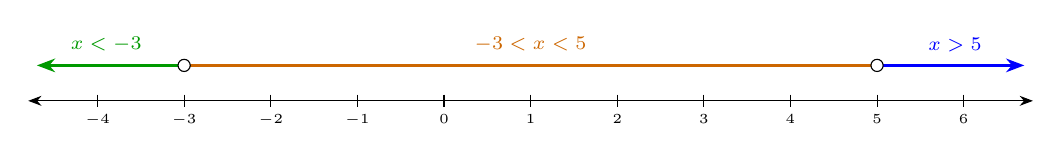
\begin{tikzpicture}[x=1.1cm]
  \draw[{Stealth}-{Stealth}] (-4.8,0) -- (6.8,0);
  \foreach \x in {-4,...,6} {
    \draw (\x,0.08) -- (\x,-0.08);
    \node[below, font=\tiny] at (\x,-0.05) {$\x$};
  }
  \draw[green!60!black, thick, {Stealth}-] (-4.7,0.45) -- (-3,0.45);
  \node[green!60!black, font=\scriptsize, above] at (-3.9,0.5) {$x < -3$};
  \draw[orange!80!black, thick] (-3,0.45) -- (5,0.45);
  \node[orange!80!black, font=\scriptsize, above] at (1,0.5) {$-3 < x < 5$};
  \draw[blue, thick, -{Stealth}] (5,0.45) -- (6.7,0.45);
  \node[blue, font=\scriptsize, above] at (5.9,0.5) {$x > 5$};
  \foreach \x in {-3,5} {
    \fill[white] (\x,0.45) circle (2.2pt);
    \draw (\x,0.45) circle (2.2pt);
  }
\end{tikzpicture}
\end{center}
\figcaption{2.7}{Representing possible solutions to quadratic inequalities on number lines}

\begin{center}
\small\setlength{\tabcolsep}{4pt}
\begin{tabular}{|p{2.7cm}|p{1.4cm}|c|c|c|l|}
\hline
\textbf{Possible Solution Regions} & \textbf{Test Values} & $\boldsymbol{x + 3}$ &
$\boldsymbol{x - 5}$ & $\boldsymbol{(x + 3)(x - 5)}$ & \textbf{Sign} \\
\hline
$x < -3$ & $-4$ & $-1$ & $-9$ & 9 & Positive \\
\hline
$-3 < x < 5$ & 3 & 6 & $-2$ & $-12$ & Negative \\
\hline
$x > 5$ & 6 & 9 & 1 & 9 & Positive \\
\hline
\end{tabular}
\end{center}

\textbf{Step 4:} Select the solution region that corresponds to the sign satisfying the
inequality.

Since $x^2 - 2x - 15 < 0$ holds for only values of $x$ for which the product of the
factors is negative (less than zero), $-3 < x < 5$ is the solution to the inequality.

\textbf{OR}

\textbf{Step 3:}

\textbf{Method 2:} Graph the quadratic inequality
\begin{center}
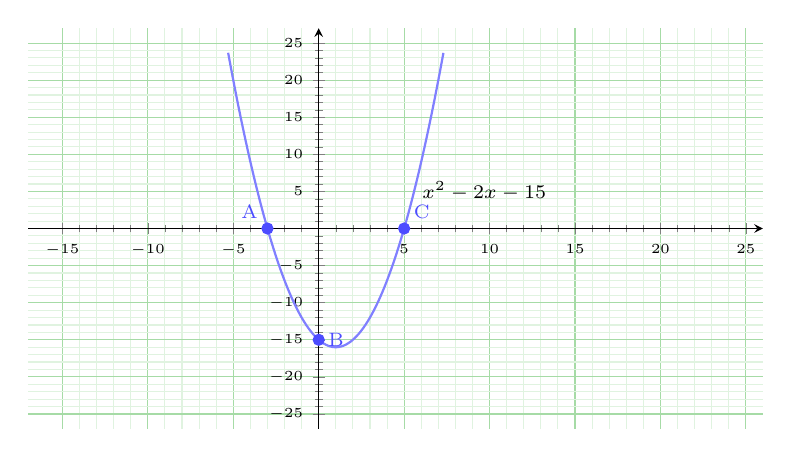
\begin{tikzpicture}
\begin{axis}[
  width=0.9\linewidth, height=0.55\linewidth,
  axis lines=middle, grid=both, minor tick num=4,
  grid style={green!60!black!35}, minor grid style={green!60!black!12},
  xmin=-17, xmax=26, ymin=-27, ymax=27,
  xtick={-15,-10,...,25}, ytick={-25,-20,...,25},
  tick label style={font=\tiny}
]
\addplot[blue!50, thick, domain=-5.3:7.3, samples=100] {x^2 - 2*x - 15};
\addplot[only marks, mark=*, blue!70] coordinates {(-3,0) (5,0) (0,-15)};
\node[blue!70, above left, font=\scriptsize] at (axis cs:-3,0) {A};
\node[blue!70, above right, font=\scriptsize] at (axis cs:5,0) {C};
\node[blue!70, right, font=\scriptsize] at (axis cs:0,-15) {B};
\node[right, font=\scriptsize] at (axis cs:5.5,5) {$x^2 - 2x - 15$};
\end{axis}
\end{tikzpicture}
\end{center}
\figcaption{2.8}{Quadratic graph of $x^2 - 2x - 15$}

\textbf{Step 4:} Identify the portion of the graph that satisfies the inequality. In this
case, the portion below the x-axis.
\begin{center}
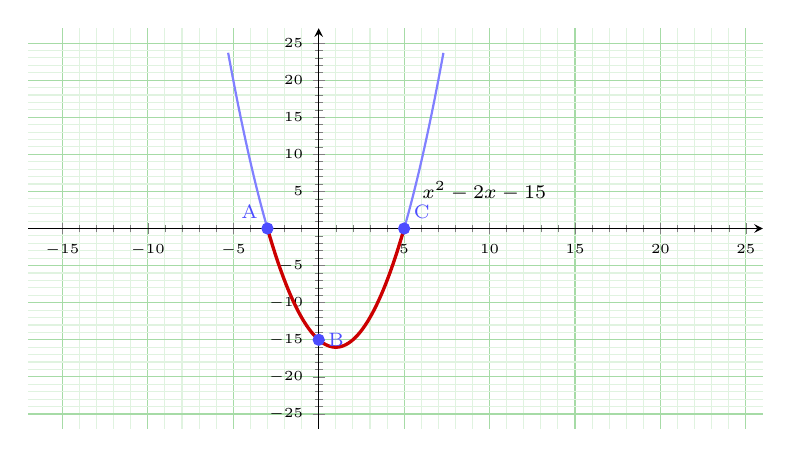
\begin{tikzpicture}
\begin{axis}[
  width=0.9\linewidth, height=0.55\linewidth,
  axis lines=middle, grid=both, minor tick num=4,
  grid style={green!60!black!35}, minor grid style={green!60!black!12},
  xmin=-17, xmax=26, ymin=-27, ymax=27,
  xtick={-15,-10,...,25}, ytick={-25,-20,...,25},
  tick label style={font=\tiny}
]
\addplot[blue!50, thick, domain=-5.3:7.3, samples=100] {x^2 - 2*x - 15};
\addplot[red!80!black, very thick, domain=-3:5, samples=60] {x^2 - 2*x - 15};
\addplot[only marks, mark=*, blue!70] coordinates {(-3,0) (5,0) (0,-15)};
\node[blue!70, above left, font=\scriptsize] at (axis cs:-3,0) {A};
\node[blue!70, above right, font=\scriptsize] at (axis cs:5,0) {C};
\node[blue!70, right, font=\scriptsize] at (axis cs:0,-15) {B};
\node[right, font=\scriptsize] at (axis cs:5.5,5) {$x^2 - 2x - 15$};
\end{axis}
\end{tikzpicture}
\end{center}
\figcaption{2.9}{Quadratic graph of $x^2 - 2x - 15$ with solution}

Thus $-3 < x < 5$
\end{example}

% Book pp. 78-79 (PDF pp. 79-80)
\begin{example}{Example 2.19}
Find the solution to the inequality $-5x^2 + 12x - 7 > 0$.

\solution
\textbf{Step 1:} Factorise the left-hand side of the inequality

$-5x^2 + 12x - 7 = (-5x + 7)(x - 1)$

Hence $(-5x + 7)(x - 1) > 0$

\textbf{Step 2:} Find the critical values

$x = \frac{7}{5}$ and $x = 1$.

\textbf{Step 3:} Represent the extreme values of the expected solution on a number line
and test them.
\begin{center}
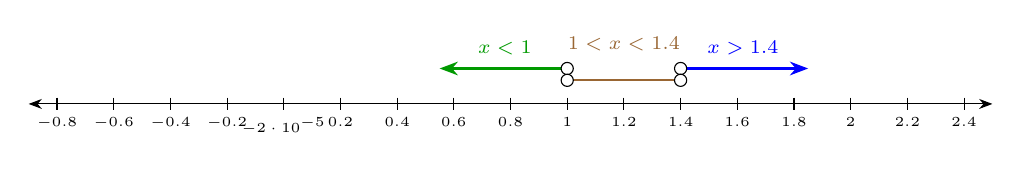
\begin{tikzpicture}[x=3.6cm]
  \draw[{Stealth}-{Stealth}] (-0.9,0) -- (2.5,0);
  \foreach \x in {-0.8,-0.6,...,2.4} {
    \draw (\x,0.08) -- (\x,-0.08);
    \node[below, font=\tiny] at (\x,-0.05) {\pgfmathprintnumber{\x}};
  }
  \draw[green!60!black, thick, {Stealth}-] (0.55,0.45) -- (1,0.45);
  \node[green!60!black, font=\scriptsize, above] at (0.78,0.5) {$x < 1$};
  \draw[brown!80!black, thick] (1,0.3) -- (1.4,0.3);
  \node[brown!80!black, font=\scriptsize, above] at (1.2,0.55) {$1 < x < 1.4$};
  \draw[blue, thick, -{Stealth}] (1.4,0.45) -- (1.85,0.45);
  \node[blue, font=\scriptsize, above] at (1.62,0.5) {$x > 1.4$};
  \fill[white] (1,0.45) circle (2.2pt); \draw (1,0.45) circle (2.2pt);
  \fill[white] (1.4,0.45) circle (2.2pt); \draw (1.4,0.45) circle (2.2pt);
  \fill[white] (1,0.3) circle (2.2pt); \draw (1,0.3) circle (2.2pt);
  \fill[white] (1.4,0.3) circle (2.2pt); \draw (1.4,0.3) circle (2.2pt);
\end{tikzpicture}
\end{center}
\figcaption{2.10}{Representing quadratic solution on number line 2}

\begin{center}
\small\setlength{\tabcolsep}{4pt}
\begin{tabular}{|p{2.7cm}|p{1.4cm}|c|c|c|l|}
\hline
\textbf{Possible Solution Regions} & \textbf{Test Values} & $\boldsymbol{-5x + 7}$ &
$\boldsymbol{x - 1}$ & $\boldsymbol{(-5x + 7)(x - 1)}$ & \textbf{Sign} \\
\hline
$x < 1$ & 0 & 7 & $-1$ & $-7$ & Negative \\
\hline
$1 < x < 1.4$ & 1.2 & 1 & 0.2 & 0.2 & Positive \\
\hline
$x > 1.4$ & 3 & $-8$ & 2 & $-16$ & Negative \\
\hline
\end{tabular}
\end{center}

\textbf{Step 4:} Select the solution region that corresponds to the sign satisfying the
inequality.

Since $-5x^2 + 12x - 7 > 0$ holds for only values of $x$ for which the product of the
factors is positive (greater than zero), $1 < x < 1.4$ is the solution to the inequality.
\end{example}

\begin{activity}{Activity 2.7 -- Graphical Solution to $-5x^2 + 12x - 7 > 0$}
Represent the solution to $-5x^2 + 12x - 7 > 0$ graphically and share the results
with a classmate.
\end{activity}

\begin{activity}{Activity 2.8 -- Research on Quadratic Inequalities}
\begin{enumerate}
  \item Conduct research on the behaviour of solutions to maximum and
  minimum curves of quadratic functions.
\end{enumerate}
\textbf{Instructions:}
\begin{enumerate}
  \item[a.] Explore the nature of the solution when a quadratic function with a
  minimum curve is:
  \begin{enumerate}
    \item[i.] greater than zero
    \item[ii.] less than zero
  \end{enumerate}
  \item[b.] Explore the nature of the solution when a quadratic function with a
  maximum curve is:
  \begin{enumerate}
    \item[i.] less than zero
    \item[ii.] greater than zero
  \end{enumerate}
  \item[c.] Include graphical representations to support your argument.
  \item[d.] Consult open education resources, YouTube, textbooks, etc.
  \item[e.] Provide references to the sources you consult and use.
\end{enumerate}
\end{activity}

% Book pp. 79-81 (PDF pp. 80-82)
\section{Solving Systems of Quadratic Inequalities}

We have explored how to solve single quadratic inequalities algebraically and
graphically. Now, we will learn how to solve systems of quadratic inequalities
(two or more quadratic inequalities) through algebra and graphing.

In finding solutions to quadratic inequalities algebraically, you solve them
simultaneously.

\begin{example}{Example 2.20}
Graph the system of quadratic inequalities $y \ge 4x^2 + 5x$, $y < -3x^2 - 7x$.

\solution
\textit{Solving the systems of inequalities simultaneously}

\textbf{Step 1:} Equate the two expressions

$4x^2 + 5x = -3x^2 - 7x$

\textbf{Step 2:} Simplify and make $x$ the subject.
\begin{align*}
  4x^2 + 3x^2 + 7x + 5x &= 0 \\
  7x^2 + 12x &= 0 \\
  x(7x + 12) &= 0 \\
  x = 0,\ x &= -\frac{12}{7}.
\end{align*}
\textbf{Step 3:} Identify whether the point of intersection is inclusive in the solution to
the systems.

Since the $y < -3x^2 - 7x$ has the strictly $<$ symbol, the points of intersection will
not satisfy this inequality.

For $y \ge 4x^2 + 5x$,

At $x = 0$, $y \ge 4(0)^2 + 5(0)$,

$y \ge 0$.

For $y < -3x^2 - 7x$,

At $x = 0$, $y < -3(0)^2 - 7(0)$,

$y < 0$

At $x = 0$, y must be 0 in both inequalities, but since the second inequality requires
$y < 0$, there is no solution at this point.

At $x = \frac{-12}{7}$, $y \ge 4\left(\frac{-12}{7}\right)^2 + 5\left(\frac{-12}{7}\right)$,

$y \ge 3\frac{3}{49}$.

At $x = 0$, $y < -3\left(\frac{-12}{7}\right)^2 - 7\left(\frac{-12}{7}\right)$,

$y < \frac{156}{49}$.

$y < 3\frac{9}{49}$.

At $x = \frac{-12}{7}$, y must be $3\frac{9}{49}$ in both inequalities, but since the second
inequality requires $y < 3\frac{9}{49}$, there is no solution at this point.
\booknote[S2-09]{$4\left(\frac{-12}{7}\right)^2 + 5\left(\frac{-12}{7}\right) = \frac{156}{49}
= 3\frac{9}{49}$, so ``$y \ge 3\frac{3}{49}$'' is a misprint; the line ``At $x = 0$,
$y < -3\left(\frac{-12}{7}\right)^2 \ldots$'' should begin ``At $x = \frac{-12}{7}$''.}

\textbf{Step 4:} State the solution

Since the points of intersection will not satisfy one of the inequalities, the solution
becomes $-1\frac{5}{7} < x < 0$. That is, the region between the points of intersection.

\medskip\noindent{\large\textbf{Solving the systems of inequalities graphically}}

\textbf{Step 1:} Draw the graphs of the two inequalities.
\begin{center}
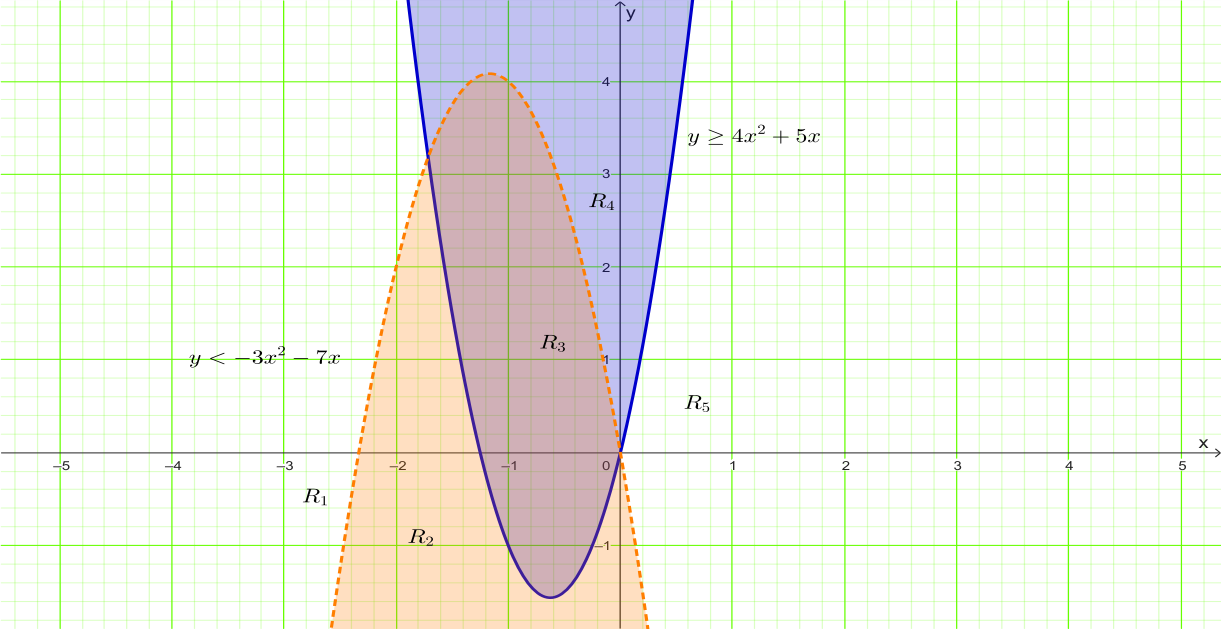
\includegraphics[width=0.9\linewidth]{figures/fig2-11.png}
\end{center}
\figcaption{2.11}{Graphical Solution to $y \ge 4x^2 + 5x$, $y < -3x^2 - 7x$}

\textbf{Step 2:} Identify the region that is common to both inequalities.

$R_3$

\textbf{Step 3:} State the solution to the system of inequalities.

$-1\frac{5}{7} < x < 0$

\textbf{Step 3:} State the conclusion.

All points in the region $R_3$ including but not exclusive to $(-1, 0)$, $(-1, 3)$
$(-0.5, 2)$, $(-1, 1)$ and $(-0.5, -1)$ are in the solution set for the system.
\end{example}

\begin{example}{Self-assessment task}
Find the solution to $y < -7x^2 - 8x + 3$ and $y > 3x^2 - 7x$.

You should find $-0.6 < x < 0.5$
\end{example}

% Book pp. 82-8x (PDF pp. 83-8x)
\section{Solving Real-Life Problems Involving Quadratic Inequalities}

Quadratic inequalities are a powerful tool used to model and solve various real-world
problems that involve limits, boundaries, or optimisation of quantities.
These inequalities describe relationships where one side of the equation is a
quadratic expression and are used in situations where the possible outcomes form
a range or region rather than a single point.

By learning how to solve quadratic inequalities, we can:
\begin{enumerate}
  \item Predict outcomes that must fall within thresholds like safety limits, financial
  losses, etc.
  \item Identify ranges of values that satisfy conditions in optimisation problems
  such as finding the most efficient design.
  \item Understand the critical points where changes in conditions occur, allowing
  for better decision-making and problem-solving.
\end{enumerate}
Let's go through these examples to see how the concept of quadratic inequalities
is useful in real-life.

\begin{example}{Example 2.21}
An artist is planning an art exhibition and needs to create rectangular canvases
with a specific aesthetic balance.

The total area available for displaying the artworks is limited to 80 square feet.
The artist wants the length of each canvas to be 2 feet less than its width.

To ensure that the artworks are visually appealing and fit within the assigned
space, determine the maximum width for each canvas such that the total area used
does not exceed 80 square feet.

\solution
\textbf{Step 1:} Represent the statement algebraically

Let w be the width of each canvas

Length of each canvas $=$ w $-\ 2$

\textbf{Step 2:} Write the equation for area of a rectangle

Since Area(A) $=$ width $\times$ length,

$A = w(w - 2)$

$A = w^2 - 2w$

\textbf{Step 3:} Set up the linear inequality

Since the space available for display is maximum 80 sq. feet, the total space
covered by the art can be less or equal to 80 square feet.

width $\times$ length $\le 80$

\textbf{Step 4:} Set up the quadratic inequality and simplify.
\begin{align*}
  w^2 - 2w &\le 80 \\
  w^2 - 2w - 80 &\le 0 \\
  (w - 10)(w + 8) &\le 0 \text{ (Sketch the inequality to confirm the required values)} \\
  \therefore -8 \le w &\le 10
\end{align*}
Since width can only be positive, the width of each canvas must be less than or
equal to 10 feet.

\textbf{Step 6:} State your conclusion

The artist can create canvases with a width up to 10 feet, ensuring the canvases fit
within the available display area at the exhibition.
\booknote[S2-10]{the book goes from Step 4 to Step 6; there is no Step 5.}
\end{example}

\begin{example}{Example 2.22}
Millicent would like to design a necklace for her mother and decides it should
resemble an eye. She makes a drawing as shown in Figure. 2.12. Identify the
systems of quadratic inequalities that helped her draw the necklace.
\begin{center}
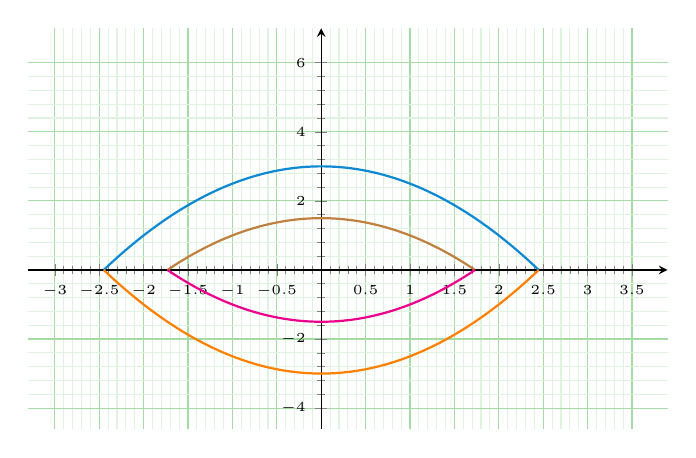
\begin{tikzpicture}
\begin{axis}[
  width=0.8\linewidth, height=0.55\linewidth,
  axis lines=middle, grid=both, minor tick num=4,
  grid style={green!60!black!35}, minor grid style={green!60!black!12},
  xmin=-3.3, xmax=3.9, ymin=-4.6, ymax=7,
  xtick={-3,-2.5,...,3.5}, ytick={-4,-2,...,6},
  tick label style={font=\tiny},
  x tick label style={/pgf/number format/fixed}
]
\addplot[cyan!70!blue, thick, domain=-2.449:2.449, samples=80] {-0.5*x^2 + 3};
\addplot[brown, thick, domain=-1.732:1.732, samples=80] {-0.5*x^2 + 1.5};
\addplot[magenta, thick, domain=-1.732:1.732, samples=80] {0.5*x^2 - 1.5};
\addplot[orange, thick, domain=-2.449:2.449, samples=80] {0.5*x^2 - 3};
\end{axis}
\end{tikzpicture}
\end{center}
\figcaption{2.12}{Necklace design}

\solution
The blue quadratic inequality curve was drawn with $y \le -0.5x^2 + 3$

The brown quadratic inequality curve was drawn with $y \ge -0.5x^2 + 1.5$

The magenta quadratic inequality curve was drawn with $y \le 0.5x^2 - 1.5$

The orange quadratic inequality curve was drawn with $y \ge 0.5x^2 - 3$
\end{example}

\begin{activity}{Activity 2.9 -- Research a Real-Life Problem}
\begin{enumerate}
  \item Identify a real-world scenario where quadratic inequalities can be
  applied. Use any of the following themes to base your research on:
  \begin{enumerate}
    \item[a.] \textbf{Agriculture:} Maximising the area of a crop field, given constraints
    such as fencing materials.
    \item[b.] \textbf{Sports:} Determining the best angle and force to kick a ball in
    football for a successful shot.
    \item[c.] \textbf{Architecture:} Designing the maximum height of an arch or
    doorway while ensuring structural safety.
    \item[d.] \textbf{Business:} Managing production costs to ensure profit margins
    while minimising loss, such as determining the optimal number
    of products to produce.
    \item[e.] \textbf{Physics:} Understanding projectile motion when an object is
    thrown into the air.
  \end{enumerate}
  \item Research how quadratic functions and inequalities play a role in this
  real-world context. Use reliable online sources, textbooks, or interview
  experts if possible.
  \item Once you've chosen your problem, model it using a quadratic inequality.

  Identify the variables in your scenario (e.g., height, distance, time, cost)
  and set up the quadratic inequality that best represents the situation.
  \item Solve the quadratic inequality you have written. Use algebraic methods
  or graphical tools to determine the solution set. You can use graphing
  software, calculators, or sketch graphs by hand to visualise the solution.
  \item Discuss the real-life implications of your solution.
  \begin{enumerate}
    \item[a.] What do the solutions of the quadratic inequality mean in terms of
    the real-world problem?
    \item[b.] What decisions can be made based on your results?
  \end{enumerate}
  \item Create a visual presentation of your findings to share with your classmates
  or teacher. Your presentation should include:
  \begin{enumerate}
    \item[a.] The real-world problem you chose.
    \item[b.] The quadratic inequality you modelled from the problem.
    \item[c.] The steps you took to solve the inequality.
    \item[d.] The real-world interpretation of the solution.
    \item[e.] Any challenges or insights you encountered while working on this
    problem.
  \end{enumerate}
\end{enumerate}
You can create a poster, a digital slide presentation or even a short video to
present your work.
\end{activity}

\section*{Extended Reading}
\begin{itemize}
  \item Baffour Ba series for schools and Colleges. (Pages 444 -- 472).
  \item Effective Elective Mathematics for Senior High School; Christian Akrong
  Hesse (Pages 202 -- 232).
  \item Effective Elective Mathematics for Senior High School, Mathematics
  Association of Ghana. (Pages 247 -- 267).
  \item Talbert, J. F., \& Heng, H. H. (1995). \textit{Additional Mathematics: Pure \&
  Applied}. Pearson Education South Asia. Page(s) 90 -- 98.
\end{itemize}

% Book pp. 86-87 (PDF pp. 87-88).  The numbering is the book's own: questions
% 13/14 and 16/17/18 are single problems that the book prints as separate items.
\section*{Review Questions}

\begin{enumerate}
\item The sum of the 2\textit{nd} and the 4\textit{th} term of a geometric sequence is 10 and
the sum of the 3\textit{nd} and 5\textit{th} term is 20. Find the first term and the common
ratio.

\item
\begin{enumerate}
  \item[a.] Given that $a_1 = 25$ and $a_n = a_{n-1} + 4$ for $n > 1$

  Find:
  \begin{enumerate}
    \item[(i)] $a_2, a_3$, and $a_4$
    \item[(ii)] a formula for $a_n$ in terms of $n$
  \end{enumerate}
  \item[b.] Use your formula for $a_n$ to deduce a formula for $S_n$, the sum of the
  first $n$ terms of the sequence $a_1, a_2, a_3, \ldots a_n$ and hence find $S_{10}$
\end{enumerate}

\item The sum of the three consecutive term of an Arithmetic Progression is $-3$
and the product is 24. Find the terms.

\item The $n$th term of an exponential sequence (G.P) is $2^{1-n}$.

Calculate:
\begin{enumerate}
  \item[a.] the sum $S_n$, of the first four terms of the sequence.
  \item[b.] the sum of the sequence to infinity.
\end{enumerate}

\item Calculate the difference between the sum to infinity of the series
$1 + \frac{1}{3} + \frac{1}{9} + \ldots$, and the sum of the first 5 terms.

\item A sequence defined by $U_1 = 2$, $U_{n+1} = 2U_n - 1$, $n = 2, 3, 4, \ldots$
\begin{enumerate}
  \item[a.] Find the first five terms of the sequence
  \item[b.] Show that $U_{n+1} = 3U_n - 2U_{n-1}$
\end{enumerate}

\item The sum of the 5\textit{th} and 9\textit{th} terms of an A.P, is $-40$ and and the
11\textit{th} term is $-32$. Find the first term and the common difference.

\item A man's salary is increased by \cedi24\,000 each year. His total salary at
the end of 14 years is \cedi65\,184\,000.

Find:
\begin{enumerate}
  \item[a.] his initial salary
  \item[b.] his salary in the 14\textit{th} year
\end{enumerate}

\item The sum of the first $n$ terms of a series is given by $(n + 1)^2 - 1$. Find the
first three terms and an expression in terms of $n$ for $U_n$, $(n > 1)$.

\item A tennis ball is released from a height $h$ cm, it rebounds one-third of the
distance it has fallen after each fall. Find the height of;
\begin{enumerate}
  \item[a.] the third bounce
  \item[b.] the $n$th bounce
\end{enumerate}

\item Find the sum of the first $n$ terms of a linear sequence whose common
difference is 2 is 120 and the sum of the $2n$ term is 440. Calculate the first
term.

\item Evaluate $\sum_{r=1}^{6} (r^2 - 2)$

\item Renie's outlet manufactures two types of clothing (shirts and trousers).
The profit is \cedi50.00 for each shirt and \cedi80.00 for each pair of
trousers.

\item Due to limited resources, the company can produce a combined total of no
more than 120 pieces. Additionally, to meet demand, they must produce at
least 20 shirts and 10 pairs of trousers. How many of each of the clothing
should be produced to make the most profit?

\item Find the solution(s) to:
\begin{enumerate}
  \item[a.] $3x^2 + 5x \ge 2$.
  \item[b.] $x^2 - 2x - 3 \ge 0$.
\end{enumerate}

\item A company determines that the cost in cedis $C$, of producing $m$ bags of
maize is $C = 170m + 150$.

\item The revenue $R$, in cedis, from selling all of the bags of maize is
$R = m^2 + 530$.

\item How many bags of maize should the company produce and sell if the
company wishes to earn a profit of at least \cedi4\,000.00?

\item Mr. Buabeng and Ms. Osei run business assembling Hyundai Toyota cars.

The cost of parts and labour needed for each type of car is shown in the
table below.
\begin{center}
\begin{tabular}{|l|c|c|}
\hline
\textbf{Car type} & \textbf{Cost of Parts (\cedi\ thousand)} & \textbf{Labour (man-hours)} \\
\hline
Hyundai & 18 & 15 \\
\hline
Toyota & 36 & 30 \\
\hline
\end{tabular}
\end{center}
The business has \cedi150 (thousand) available to buy parts each week.

However, the total labour available each week is 85 man-hours. If they
make $h$ of Hyundai and $t$ of Toyota each week:
\begin{enumerate}
  \item[a.] Write down all the inequalities on $h$ and $t$.
  \item[b.] Determine the solution to the set of inequalities.
\end{enumerate}
\end{enumerate}


\chapter{Polynomial Functions}
% Book p. 89 (PDF p. 90)
\section*{Modelling with Algebra}
\subsection*{Application of Algebra}

\subsubsection*{Introduction}

This lesson is continuation of what we learnt in year one functions. We will
explore the properties, graphing techniques and basic theorems of polynomial
functions. Polynomial functions are crucial in mathematics and have applications
in science, engineering and economics. It covers factorising, finding zeros,
graphing, Descartes' Rule of Signs, Fundamental Theorem of Algebra and Linear
and Quadratic Factor Theorems. By the end of the section, you will have a deeper
understanding of polynomial functions and be prepared to solve a variety of
mathematical problems.

\begin{keyideas}
\begin{itemize}
  \item \textbf{Factorising polynomials} involves linear and irreducible quadratic
  factors.
  \item \textbf{Factors} and \textbf{zeros} are variables that make a
  \textbf{polynomial function} equal to \textbf{zero}.
  \item Graphing polynomials with higher degrees reveal complex shapes, key
  features, and roots.
  \item The \textbf{degree} of a polynomial function determines the maximum number
  of solutions a function could have and the number of times a function will
  cross the x-axis when graphed.
  \item The \textbf{degree} of a polynomial function is the total number of
  \textbf{factors}.
\end{itemize}
\end{keyideas}

% Book pp. 90-97 (PDF pp. 91-98)
\section{Finding Factors and Zeros of Polynomial Functions}

\begin{activity}{Activity 3.1: Revision of finding quadratic factors}
In pairs or small groups or individually, perform these activities.
\begin{enumerate}
  \item Factorise the following quadratic expressions:
  \begin{enumerate}
    \item[a.] $y^2 + 3y + 2$
    \item[b.] $3y^2 + 11y + 10$
    \item[c.] $6x^2 + 5x + 1$
    \item[d.] $x^2 - 9$
  \end{enumerate}
  \item Write down the factorising process clearly, showing each step taken to
  arrive at the factors.
  \item Exchange your work with other groups or peers to compare answers.
  \item Discuss any differences in methods used and validate the correctness of
  each group's results.
\end{enumerate}
\end{activity}

An expression $(\boldsymbol{x + y})$ is a factor if you can multiply it by another
expression $\boldsymbol{(e + f)}$ to get the original expression
$(\boldsymbol{ex + fx + ey + fy})$. In simple terms, if you can find two or more
expressions that multiply together to make a certain expression, then those are
its factors.

For example, $(x + 2)(x - 3)$ are factors of $x^2 - x - 6$ because expanding
$(x + 2)(x - 3)$:

$x(x - 3) + 2(x - 3)$

$x^2 - 3x + 2x - 6$

$x^2 - x - 6$

Therefore, we see that $(x + 2)(x - 3)$ is indeed equal to $x^2 - x - 6$ confirming
that they are factors of the expression. If you found activity 3.1 challenging, use
the task below to help you.

To \textbf{factorise quadratics} of the form $ax^2 + bx + c$:

\medskip
\noindent\textbf{Example}
\begin{center}
\renewcommand{\arraystretch}{1.3}
\begin{tabular}{|p{0.6\linewidth}|p{0.32\linewidth}|}
\hline
\textbf{Task} & $\boldsymbol{2x^2 + 7x + 6}$ \\
\hline
\textbf{Task 1}\newline
Find two numbers that multiply to give ac (the product of a and c) and add to give b.
& $a = 2$, $b = 7$ and $c = 6$\newline
$ac = 2 \times 6 = 12$\newline
$4 + 3 = 7$ and $4 \times 3 = 12$ \\
\hline
\textbf{Task 2}\newline
Rewrite the middle term using these two numbers as coefficients of x.
& $2x^2 + 4x + 3x + 6$ \\
\hline
\textbf{Task 3}\newline
If the polynomial has four terms, group the terms in pairs.
& $(2x^2 + 4x) + (3x + 6)$ \\
\hline
\textbf{Task 4}\newline
Factorise out the common factor from each group.
& $2x(x + 2) + 3(x + 2)$ \\
\hline
\textbf{Task 5}\newline
Look for a common binomial factor and factorise it out and you have the
factorised solution.
& $(2x + 3)(x + 2)$ \\
\hline
\end{tabular}
\end{center}

\subsection{Factor Theorem and Remainder Theorem}

In addition to quadratic functions, there are several other types of polynomial
functions that can be factorised using the Factor Theorem and the Remainder
Theorem. Remember that if $(x \pm h)$ is a factor of a polynomial, then the remainder
will be zero. Conversely, if the remainder is zero, then $(x \pm h)$ is a factor.

Here are some common types of polynomials:

\subsection{Types of Polynomials}
\begin{enumerate}
  \item \textbf{Cubic Polynomials:} Polynomials of \textit{degree} three, in the form:
  $f(x) = ax^3 + bx^2 + cx + d$
  \item \textbf{Quartic Polynomials:} Polynomials of degree four, in the form:\\
  $f(x) = ax^4 + bx^3 + cx^2 + dx + e$
  \item \textbf{Quintic Polynomials:} Polynomials of degree five, in the form:\\
  $f(x) = ax^5 + bx^4 + cx^3 + dx^2 + ex + f$
\end{enumerate}

\begin{activity}{Activity 3.2: Revision on factorisation}
In groups or individually, use the idea of the factor and remainder theorems to
find the factors or the remainders of the following polynomials.
\begin{enumerate}
  \item Find the remainder when:
  \begin{enumerate}
    \item[a.] $f(x) = 3x^3 - 4x^2 + 2x + 3$ is divided by $(x + 1)$
    \item[b.] $f(x) = 8x^3 - 3x^2 + 6x + 4$ is divided by $(x - 2)$
    \item[c.] $f(x) = 7x^3 + 3x^2 - x + 6$ is divided by $(x + 3)$
    \item[d.] $f(x) = x^3 - x^2 + x + 1$ is divided by $(x - 1)$
  \end{enumerate}
  \item
  \begin{enumerate}
    \item[a.] show that $x + 2$ is a factor of $f(x) = x^3 - 2x^2 - 5x + 6$
    \item[b.] show that $x - 3$ is a factor of $f(x) = x^3 - 3x^2 - 4x + 12$
  \end{enumerate}
  \item Compare your answers with other groups.
\end{enumerate}
\end{activity}

\subsection{Zero-Product Property}

This property of real numbers says that if you multiply two numbers together
and the result is zero, then at least one of those numbers must be zero. In simpler
terms, if you have two numbers, \textbf{a} and b, and when you multiply them
(a$\times$b), and you get zero, it means that either $a$ is zero, or $b$ is zero or
both are zero. This property helps us to find the \textbf{zeros} or \textbf{roots} of
functions of quadratic functions.

The \textbf{zeros} or \textbf{roots} of a function are the values of the input (usually
represented as x) that make the function equal to zero. In other words, if you have
a function f(x), the zeros are the values of x for which f(x) $=$ 0. For example,
given the function $f(x) = 2x^2 - x - 6$, You:
\begin{enumerate}
  \item equate f(x) $=$ 0

  $2x^2 - x - 6 = 0$
  \item factorise the function

  $2x^2 - 4x + 3x - 6 = 0$

  $2x(x - 2) + 3(x - 2) = 0$

  $(2x + 3)(x - 2) = 0$

  Either $(2x + 3) = 0$ or $(x - 2) = 0$
  \item find the solution for each factor

  $(2x + 3) = 0$

  $2x = -3$

  $x = -\frac{3}{2}$

  $(x - 2) = 0$

  $x = 0 - 2$

  $x = 2$
\end{enumerate}
Therefore, the zeros, or roots, of the function $f(x) = 2x^2 - x - 6$ are
$x = -\frac{3}{2}$ and $x = 2$ because both values make the function equal to zero.

We will apply the Zero-Product Property to solve polynomial equations in the
next task.

\subsection{Solving a Polynomial Equation}

There are a number of ways that can be used to find the zeros, or the roots, of
polynomial functions. We can use a calculator, plot a graph, use GeoGebra
(software) and we can also calculate by using the zero property.

\textit{To find the zeros, or roots, by the calculation method:}

Step 1: use the factor theorem approach to factorise the expression completely.

Step 2: equate each factor to 0 and solve.

In pairs or in groups, let's work through the following examples using the steps
above.

\begin{example}{Example 3.1}
Find the zeros of the cubic function $f(x) = x^3 - 2x^2 - 5x + 6$

\solution
$x^3 - 2x^2 - 5x + 6 = 0$

Possible factors of $6 = \pm 1, \pm 2, \pm 3, \pm 6$

Testing with these factors,

When x $=$ 1,

$f(x) = (1)^3 - 2(1)^2 - 5(1) + 6$

$f(x) = 1 - 2 - 5 + 6$

$f(x) = 0$

$\therefore (x - 1)$ is a factor. If x=1 was not a factor, try another option, eg x=-1.

Using the long division method:
\[
\begin{array}{r@{\;}r}
 & x^2 - x - 6 \\ \cline{2-2}
x - 1\,\big) & x^3 - 2x^2 - 5x + 6 \\
 & \underline{-(x^3 - x^2 + 0x + 0)} \\
 & -x^2 - 5x + 6 \\
 & \underline{-(-x^2 + x - 0)} \\
 & -6x + 6 \\
 & \underline{-(-6x + 6)} \\
 & 0
\end{array}
\]
Factorising, $x^2 - x - 6$

$x^2 - 3x + 2x - 6$

$(x^2 - 3x) + (2x - 6)$

$x(x - 3) + 2(x - 3)$

$(x + 2)(x - 3)$

$\therefore \mathrm{f}(\mathrm{x}) = (x - 1)(x + 2)(x - 3)$

$f(x) = 0$

$(x - 1)(x + 2)(x - 3) = 0$

For $(x - 1) = 0$

$x = 1$

For $(x + 2) = 0$

$x = -2$

For $(x - 3) = 0$

$x = 3$

Hence the zeros are when x $= -2, 1, 3$
\end{example}

\begin{example}{Example 3.2}
Find the roots, or zeros, of the cubic function $f(x) = x^3 + x^2 - 10x + 8$

\solution
$x^3 + x^2 - 10x + 8 = 0$

Possible factors of $8 = \pm 1, \pm 2, \pm 4, \pm 8$

Testing with these factors,

When x $=$ 1,

$f(x) = (1)^3 + (1)^2 - 10(1) + 8$

$f(x) = 1 + 1 - 10 + 8$

$f(x) = 0$

$\therefore (x - 1)$ is a factor.

Using the long division method:
\[
\begin{array}{r@{\;}r}
 & x^2 + 2x - 8 \\ \cline{2-2}
x - 1\,\big) & x^3 + x^2 - 10x + 8 \\
 & \underline{-(x^3 - x^2 + 0x + 0)} \\
 & 2x^2 - 10x + 8 \\
 & \underline{-(2x^2 - 2x - 0)} \\
 & -8x + 8 \\
 & \underline{-(-8x + 8)} \\
 & 0
\end{array}
\]
Factorising, $x^2 + 2x - 8$

$x^2 + 4x - 2x - 8$

$(x^2 + 4x) + (2x - 8)$

$x(x + 4) - 2(x + 4)$

$(x + 4)(x - 2)$

$\therefore \mathrm{f}(\mathrm{x}) = (x - 1)(x - 2)(x + 4)$

$f(x) = 0$

$(x - 1)(x - 2)(x + 4) = 0$

For $(x - 1) = 0$

$x = 1$

For $(x - 2) = 0$

$x = 2$

For $(x + 4) = 0$

$x = -4$

Hence the roots, or zeros, are when x $= -4, 2, 1$
\end{example}

\begin{example}{Example 3.3}
Find the zeros of the cubic function. $f(x) = x^3 - 3x^2 - 4x + 12$

\solution
$x^3 - 3x^2 - 4x + 12 = 0$

Possible factors of $12 = \pm 1, \pm 2, \pm 3, \pm 4, \pm 6, \pm 12$

Testing with these factors,

When x $=$ 1,

$f(x) = (1)^3 - 3(1)^2 - 4(1) + 12$

$f(x) = 1 - 3 - 4 + 12$

$f(x) = 6$

$\therefore (x - 1)$ is not a factor and we need to try another potential factor.

When $x = 2$,

$f(x) = (2)^3 - 3(2)^2 - 4(2) + 12$

$f(x) = 8 - 12 - 8 + 12$

$f(x) = 0$

$\therefore (x - 2)$ is a factor.

Using the long division method:
\[
\begin{array}{r@{\;}r}
 & x^2 - x - 6 \\ \cline{2-2}
x - 2\,\big) & x^3 - 3x^2 - 4x + 12 \\
 & \underline{-(x^3 - 2x^2 + 0x + 0)} \\
 & -x^2 - 4x + 12 \\
 & \underline{-(x^2 + 2x - 0)} \\
 & -6x + 12 \\
 & \underline{-(6x + 12)} \\
 & 0
\end{array}
\]
\booknote[S3-01]{the book's long division subtracts $(x^2 + 2x - 0)$ and $(6x + 12)$;
the lines being subtracted are $(-x^2 + 2x - 0)$ and $(-6x + 12)$. The quotient
$x^2 - x - 6$ is correct.}

Factorising, $x^2 - x - 6$

$x^2 - 3x + 2x - 6$

$(x^2 - 3x) + (2x - 6)$

$x(x - 3) + 2(x - 3)$

$(x + 2)(x - 3)$

$\therefore \mathrm{f}(\mathrm{x}) = (x - 2)(x + 2)(x - 3)$

$f(x) = 0$

$(x - 2)(x + 2)(x - 3) = 0$

For $(x - 2) = 0$

$x = 2$

For $(x + 2) = 0$

$x = -2$

For $(x - 3) = 0$

$x = 3$

Hence the zeros are when x $= -2, 2, 3$
\end{example}

Following the remainder theorem is the Rational Zero Theorem which helps to
identify exactly which of the factor will give us zero.

% Book pp. 97-102 (PDF pp. 98-103)
\subsection{The Rational Zero Theorem}

The Rational Zero Theorem helps us identify potential rational zeros of a
polynomial by looking at the factors of two specific parts of the polynomial:
\begin{enumerate}
  \item Factors of the Constant Term: This is the term without a variable (the last
  number in the polynomial when arranged in descending powers).
  \item Factors of the Leading Coefficient: This is the coefficient (the number in
  front of the term) of the term with the highest power of $x$.
\end{enumerate}

\noindent\textbf{\textit{Steps to Find Possible Rational Zeros}}
\begin{enumerate}
  \item Identify the Constant Term and Leading Coefficient.

  For example, in the polynomial $4x^3 + 7x^2 + 2x + 5$:

  The constant term is 5.

  The leading coefficient is 4.
  \item List the Factors.

  Factors of the Constant Term (5): These are: $\pm 1$, $\pm 5$

  Factors of the Leading Coefficient (4): These are $\pm 1$, $\pm 2$, $\pm 4$.
  \item Create Possible Rational Zeros.

  To find the possible rational zeros, take each factor of the constant term and
  divide it by each factor of the leading coefficient.

  Possible rational zeros for our example would be:

  From $\pm 1$: $\frac{1}{1}, -\frac{1}{1}, \frac{1}{2}, -\frac{1}{2}, \frac{1}{4},
  \frac{-1}{4}, = \pm 1, \pm\frac{1}{2}, \pm\frac{1}{4}$,

  From $\pm 5$: $\frac{5}{1} - \frac{5}{1}, \frac{5}{2}, -\frac{5}{2}, \frac{5}{4},
  \frac{-5}{4}, = \pm 5, \pm\frac{5}{2}, \pm\frac{5}{4}$
  \item List of Possible Rational Zeros:

  Combining all these, the possible rational zeros for our polynomial are:

  $\pm 1, \pm 5, \pm\frac{1}{2}, \pm\frac{1}{4}, , \pm\frac{5}{2}, \pm\frac{5}{4}$
\end{enumerate}
Now that we have a list of possible rational zeros, we can use the Factor Theorem
to test each one.
\begin{enumerate}
  \item[a.] For each rational number c from the list, substitute it into the polynomial
  f(x)
  \item[b.] If f($c$) $=$ 0, then c is a zero of the polynomial.
\end{enumerate}

\begin{example}{Example 3.4}
In groups or individually, use the rational zeros theorem to list all the possible
rational zeros.
\begin{enumerate}
  \item[a.] $6x^3 + 15x^2 - 8x + 2$
  \item[b.] $x^3 + x^2 - 2x - 5$
  \item[c.] $3x^3 + x^2 + x - 5$
  \item[d.] $6x^3 - 4x^2 + 17$
\end{enumerate}
\booknote[S3-02]{the solution below works parts b and c for different
polynomials, $x^3 + x^2 - 2x - 8$ and $9x^3 + x^2 + x - 10$, from those printed
in the question.}

\solution
\begin{enumerate}
  \item[a.] $6x^3 + 15x^2 - 8x + 2$

  The constant term is 2.

  The leading coefficient is 6.

  Factors of the Constant Term (2): These are.$\pm 1$, $\pm 2$

  Factors of the Leading Coefficient (6): These are $\pm 1$, $\pm 2$, $\pm 3$, $\pm 6$.

  Possible Rational Zeros:

  From $\pm 1$: $\frac{1}{1}, -\frac{1}{1}, \frac{1}{2}, -\frac{1}{2}, \frac{1}{3},
  \frac{-1}{3}, \frac{1}{6}, -\frac{1}{6} = \pm 1, \pm\frac{1}{2}, \pm\frac{1}{3},
  \pm\frac{1}{6}$,

  From $\pm 2$: $\frac{2}{2}, -\frac{2}{2}, \frac{2}{3}, \frac{-2}{3}, \frac{2}{6},
  -\frac{2}{6} = \pm 1, \pm\frac{2}{3}, \pm\frac{1}{6}$,
  \booknote[S3-03]{the book's ``From $\pm 2$'' line omits $\frac{2}{1}$ and ends
  in $\pm\frac{1}{6}$; dividing $\pm 2$ by $1, 2, 3, 6$ gives $\pm 2, \pm 1,
  \pm\frac{2}{3}, \pm\frac{1}{3}$, and no combined list is given for this part.}

  \item[b.] $x^3 + x^2 - 2x - 8$

  The constant term is $-8$.

  The leading coefficient is 1.

  Factors of the Constant Term (-8): These are.$\pm 1$, $\pm 2$, $\pm 4$, $\pm 8$

  Factors of the Leading Coefficient (1): These are $\pm 1$.

  Possible Rational Zeros:

  From $\pm 1$: $\frac{1}{1}, -\frac{1}{1} = \pm 1$

  From $\pm 2$: , $\frac{2}{1}, -\frac{2}{1} = \pm 2$

  From $\pm 4$: $\frac{4}{1}, -\frac{4}{1}, = \pm 4$

  From $\pm 8$: , $\frac{8}{1}, -\frac{8}{1} = \pm 8$,,

  Possible Rational Zeros (combined): $\pm 1, \pm 2, \pm 4, \pm 8$

  \item[c.] $9x^3 + x^2 + x - 10$

  The constant term is $-10$.

  The leading coefficient is 9.

  Factors of the Constant Term (-10): These are.$\pm 1$, $\pm 2$, $\pm 5$, $\pm 10$

  Factors of the Leading Coefficient (9): These are $\pm 1$, $\pm 3$, $\pm 9$.

  Possible Rational Zeros:

  From $\pm 1$: $\frac{1}{1}, -\frac{1}{1}, \frac{1}{3}, -\frac{1}{3}, \frac{1}{9},
  -\frac{1}{9} = \pm 1, \pm\frac{1}{3}, \pm\frac{1}{9}$

  From $\pm 2$: $\frac{2}{1}, -\frac{2}{1}, \frac{2}{3}, -\frac{2}{3}, \frac{2}{9},
  -\frac{2}{9} = \pm 2, \pm\frac{2}{3}, \pm\frac{2}{9}$

  From $\pm 4$: $\frac{5}{1}, -\frac{5}{1}, \frac{5}{3}, -\frac{5}{3}, \frac{5}{9},
  -\frac{5}{9} = \pm 5, \pm\frac{5}{3}, \pm\frac{5}{9}$
  \booknote[S3-04]{the book heads this line ``From $\pm 4$''; it should be
  ``From $\pm 5$'', as the fractions show.}

  From $\pm 10$: , $\frac{10}{1}, -\frac{10}{1}, \frac{10}{3}, -\frac{10}{3},
  \frac{10}{9}, -\frac{10}{9} = \pm 10, \pm\frac{10}{3}, \pm\frac{10}{9}$

  Possible Rational Zeros (combined): $\pm 1, \pm 2, \pm 5, \pm 10\ \pm\frac{1}{3},
  \pm\frac{1}{9}, \pm\frac{2}{3}, \pm\frac{2}{9}, \pm\frac{5}{3}, \pm\frac{5}{9},
  \pm\frac{10}{3}, \pm\frac{10}{9}$

  \item[d.] $6x^3 - 4x^2 + 17$

  The constant term is 17.

  The leading coefficient is 6.

  Factors of the Constant Term (17): These are.$\pm 1$, $\pm 17$

  Factors of the Leading Coefficient (6): These are $\pm 1$, $\pm 2$, $\pm 3$, $\pm 6$.

  Possible Rational Zeros\textbf{:}

  From $\pm 1$: $\frac{1}{1}, -\frac{1}{1}, \frac{1}{2}, -\frac{1}{2}, \frac{1}{3},
  -\frac{1}{3}, \frac{1}{6}, -\frac{1}{6} = \pm 1, \pm\frac{1}{2}, \pm\frac{1}{3},
  \pm\frac{1}{6}$

  From $\pm 17$: $\frac{17}{1}, -\frac{17}{1}, \frac{17}{2}, -\frac{17}{2},
  \frac{17}{3}, -\frac{17}{3}, \frac{17}{6}, -\frac{17}{6} = = \pm 17,
  \pm\frac{17}{2}, \pm\frac{17}{3}, \pm\frac{17}{6}$

  Possible Rational Zeros (combined): $\pm 1, \pm 17, \pm\frac{1}{2}, \pm\frac{1}{3},
  \pm\frac{1}{6}, \pm\frac{17}{2}, \pm\frac{17}{3}, \pm\frac{17}{6}$
\end{enumerate}
\end{example}

\subsection{Using the rational zero theorem to find the zeros of a polynomial function}

\noindent\textit{Steps to Follow:}
\begin{enumerate}
  \item Identify Possible Rational Zeros

  Use the Rational Zero theorem to list all possible rational zeros. These are
  of the form $p$ and $q$, where $p$ is a factor of the constant term (the last term of
  the polynomial) and $q$ is a factor of the leading coefficient (the coefficient of
  the term with the highest degree).
  \item Substitute and Evaluate
  \begin{enumerate}
    \item[a.] Substitute each possible rational zero into the polynomial function.
    \item[b.] Calculate the value of the polynomial for each substitution.
  \end{enumerate}
  \item Determine Actual Zeros
  \begin{enumerate}
    \item[a.] Identify which substitutions result in a value of zero.
    \item[b.] The values for which the polynomial equals zero are the rational zeros
    of the function.
  \end{enumerate}
\end{enumerate}

\begin{example}{Example 3.5}
Given the polynomial $3x^3 + 8x^2 + 7x + 2$
\begin{enumerate}
  \item List the factors of the constant term and leading coefficient.
  \item Determine possible rational zeros
  \item Substitute each value into the polynomial to find which ones yield zero.
\end{enumerate}

\solution
The constant term is 2.

The leading coefficient is 3.

Factors of the Constant Term (2): These are.$\pm 1$, $\pm 2$

Factors of the Leading Coefficient (3): These are $\pm 1$, $\pm 3$.

Possible Rational Zeros:

From $\pm 1$: $\frac{1}{1}, -\frac{1}{1}, \frac{1}{3}, -\frac{1}{3} = \pm 1,
\pm\frac{1}{3}$

From $\pm 2$: $\frac{2}{1}, -\frac{2}{1}, \frac{2}{3}, -\frac{2}{3}, = = \pm 2,
\pm\frac{2}{3}$

Possible Rational Zeros (combined): $\pm 1, \pm 2, \pm\frac{1}{3}, \pm\frac{2}{3}$

Substitute and evaluate:

$3x^3 + 8x^2 + 7x + 2$

For $x = \pm 1$:

$x = 1$

$3(1)^3 + 8(1)^2 + 7(1) + 2$

$3 + 8 + 7 + 2 = 20$

$\boldsymbol{x} = -1$

$3(-1)^3 + 8(-1)^2 + 7(-1) + 2$

$-3 + 8 - 7 + 2 = 0$

For $x = \pm 2$

$x = 2$

$3(2)^3 + 8(2)^2 + 7(2) + 2$

$24 + 32 + 14 + 2 = 71$

$x = -2$

$3(-2)^3 + 8(-2)^2 + 7(-2) + 2$

$-24 + 32 - 14 + 2 = -4$

For $\pm\frac{1}{3}$

$x = \frac{1}{3}$

$3\left(\frac{1}{3}\right)^3 + 8\left(\frac{1}{3}\right)^2 + 7\left(\frac{1}{3}\right) + 2$

$\frac{1}{9} + \frac{8}{9} + \frac{7}{3} + 2 = \frac{16}{3}$

$x = -\frac{1}{3}$

$3\left(-\frac{1}{3}\right)^3 + 8\left(-\frac{1}{3}\right)^2 + 7\left(-\frac{1}{3}\right) + 2$

$-\frac{1}{9} + \frac{8}{9} - \frac{7}{3} + 2 = \frac{4}{9}$

For $\pm\frac{2}{3}$

$x = \frac{2}{3}$

$3\left(\frac{2}{3}\right)^3 + 8\left(\frac{2}{3}\right)^2 + 7\left(\frac{2}{3}\right) + 2$

$\frac{8}{9} + \frac{32}{9} + \frac{14}{3} + 2 = \frac{100}{9}$

$x = -\frac{2}{3}$

$3\left(-\frac{2}{3}\right)^3 + 8\left(-\frac{2}{3}\right)^2 + 7\left(-\frac{2}{3}\right) + 2$

$-\frac{8}{9} + \frac{32}{9} - \frac{14}{3} + 2 = 0$

The values $1, 2, -2, \frac{1}{3}, -\frac{1}{3}, \frac{2}{3}$ did not yield zero and are
not zeros of the function.

However, $-1$ and $-\frac{2}{3}$, yielded zero and therefore represent the zeros of
the function
\end{example}

% Book pp. 102-111 (PDF pp. 103-112)
\section{Sketching Polynomial Functions with Degrees Higher Than 2}

\begin{enumerate}
  \item In mathematics, the terms ``sketch'' and ``draw'' have distinct meanings.
  \item Sketch is a rough representation of a graph or function without precise
  measurements, used to illustrate its behaviour. It often lacks scales and
  coordinates.
  \item Draw, on the other hand, creates a more accurate representation with
  specific values, scales, and tools, providing a detailed visualization of a
  mathematical function or data set.
\end{enumerate}

We will be sketching polynomial functions with a degree higher than 2.

These will be cubics, quartics etc.

To sketch a polynomial of degree greater than 2, for example, $ax^3 + bx^2 + cx + d$,
we:

\textbf{Step 1:} Determine the sign ($+$ or -) of \textbf{a}; if a $>$ 0 or a $<$ 0

If a $<$ 0, the curve will have the shape:
\booknote[S3-05]{the book prints ``a $<$ 0'' above both Figure 3.1 and
Figure 3.2, and both figures show the shape for $a > 0$ (rising from bottom left
to top right). The first should read ``a $>$ 0''; the second figure should be the
reflected shape, falling from top left to bottom right.}
\begin{center}
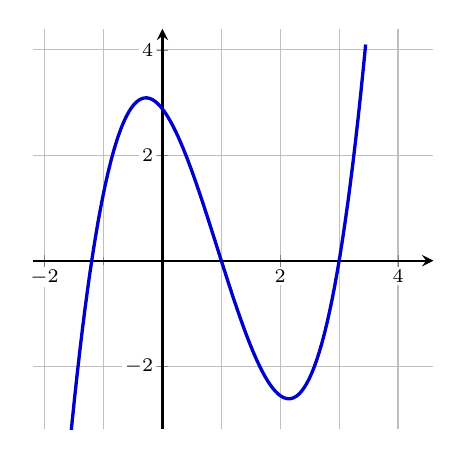
\begin{tikzpicture}
\begin{axis}[
  width=0.55\linewidth, height=0.55\linewidth,
  axis lines=middle, grid=both, minor tick num=1,
  xmin=-2.2, xmax=4.6, ymin=-3.2, ymax=4.4,
  xtick={-2,0,2,4}, ytick={-2,2,4},
  tick label style={font=\scriptsize}, ticklabel style={fill=white, inner sep=1pt},
  axis line style={thick},
]
\addplot[blue!80!black, very thick, samples=120, domain=-1.75:3.45]
  {0.8*(x+1.2)*(x-1)*(x-3)};
\end{axis}
\end{tikzpicture}
\end{center}
\figcaption{3.1}{Curve of a polynomial}

If a $<$ 0, the curve will have the shape:
\begin{center}
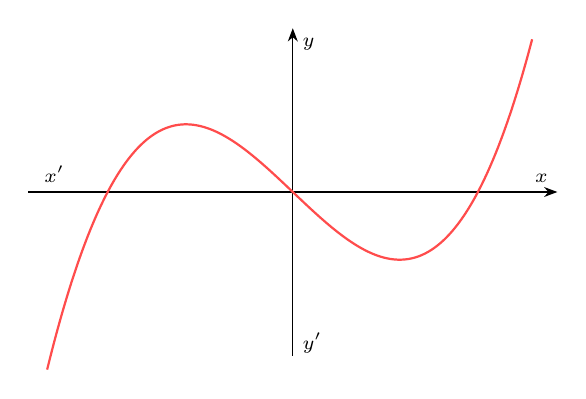
\begin{tikzpicture}[scale=0.8]
  \draw[-{Stealth}] (-4.2,0) -- (4.2,0) node[above left, font=\scriptsize] {$x$};
  \draw[-{Stealth}] (0,-2.6) -- (0,2.6) node[below right, font=\scriptsize] {$y$};
  \node[font=\scriptsize, above right] at (-4.1,0) {$x'$};
  \node[font=\scriptsize, right] at (0,-2.4) {$y'$};
  \draw[red!70, thick, samples=100, domain=-3.9:3.8, smooth]
    plot (\x, {0.11*\x*\x*\x - 0.95*\x});
\end{tikzpicture}
\end{center}
\figcaption{3.2}{Curve of a polynomial}

\textbf{Step 2:} Use the factor theorem or any known method to find the zeros of the
polynomial

\textbf{Step 3:} Find the y- intercept of the function by substituting x $=$ 0 into the
given polynomial function. (Note that this equates to the constant.)

\textbf{Step 4:} Find the intervals of the curve based on the zeros obtained

\textbf{Step 5:} Sketch the curve.

Individually, or in groups, let's use the steps for sketching polynomials to solve
the examples below.

\begin{example}{Example 3.6}
Sketch the curve $2x^3 + 3x^2 - 5x - 6$

\solution
\textbf{Step 1:} a is 2, which is greater than 0. Therefore, we know the shape that the
curve will take. The extremes will go from bottom left to top right.

\textbf{Step 2:} Using the factor theorem, the factors of the constant, - 6 are
$\pm 1, \pm 2, \pm 3, \pm 6$

Testing when x $=$ - 1, we have:

$2(-1)^3 + 3(-1)^2 - 5(-1) - 6 = -2 + 3 + 5 - 6 = 0$

Which means $(x + 1)$ is a factor.

We can use long division to find the other factors.
\[
\begin{array}{r@{\;}r}
 & 2x^2 + x - 6 \\ \cline{2-2}
x + 1\,\big) & 2x^3 + 3x^2 - 5x - 6 \\
 & \underline{-(2x^3 + 2x^2 + 0 + 0)} \\
 & x^2 - 5x - 6 \\
 & \underline{-(x^2 + x + 0)} \\
 & (-6x - 6) \\
 & \underline{-6x - 6}
\end{array}
\]
Factorising:

$2x^2 + x - 6$

$2x^2 + 4x - 3x - 6$

$2x(x + 2) - 3(x + 2)$

$(2x - 3)(x + 2)$

Factors are:

$(x + 1)(2x - 3)(x + 2)$

The zeros:

$(x + 1)(2x - 3)(x + 2) = 0$

$x = -1$, $x = -2$, $x = \frac{3}{2}$

\textbf{Step 3:} y intercept

When x $=$ 0

$2(0)^3 + 3(0)^2 - 5(0) - 6 = -6$

\textbf{Step 4}: finding the intervals using the zeros
\begin{center}
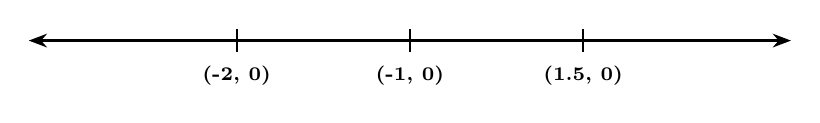
\begin{tikzpicture}[x=2.2cm]
  \draw[{Stealth}-{Stealth}, thick] (-0.7,0) -- (3.7,0);
  \foreach \x/\l in {0.5/{(-2, 0)}, 1.5/{(-1, 0)}, 2.5/{(1.5, 0)}} {
    \draw[thick] (\x,0.15) -- (\x,-0.15);
    \node[below, font=\scriptsize\bfseries] at (\x,-0.2) {\l};
  }
\end{tikzpicture}
\end{center}
The intervals are:
\begin{enumerate}
  \item $-2 < x$
  \item $-2 < x < -1$
  \item $-1 < x < 1.5$
  \item $x > 1.5$
\end{enumerate}
\booknote[S3-06]{the first interval is printed as $-2 < x$ (and $-1 < x$ in
Examples 3.7 and 3.8); the interval to the left of the first zero is $x < -2$
(respectively $x < -1$), as the table headings below show.}

Next is to determine the signs or test for the signs in each of the intervals obtained

\begin{center}
\small\renewcommand{\arraystretch}{1.2}
\begin{tabular}{|p{0.2\linewidth}|p{0.15\linewidth}|p{0.15\linewidth}|p{0.15\linewidth}|p{0.15\linewidth}|}
\hline
\textbf{Interval} & {\boldmath$-2 > x$} & {\boldmath$-2 < x < -1$} & {\boldmath$-1 < x < 1.5$} & {\boldmath$x > 1.5$} \\
\hline
Chosen values (you can choose any number within the interval)
& \centering\textbf{-3} & \centering\textbf{-1.5} & \centering\textbf{1} & \centering\textbf{2} \tabularnewline
\hline
$y$ value (substitute your chosen number into the given function)
& \centering $2(-3)^3 + 3(-3)^2 - 5(-3) - 6$ \par\medskip \textbf{= -18}
& \centering $2(-1.5)^3 + 3(-1.5)^2 - 5(-1.5) - 6$ \par\medskip \textbf{= 1.5}
& \centering $2(1)^3 + 3(1)^2 - 5(1) - 6$ \par\medskip \textbf{= -6}
& \centering $2(2)^3 + 3(2)^2 - 5(2) - 6$ \par\medskip \textbf{= 12} \tabularnewline
\hline
Sign & \centering Negative & \centering Positive & \centering Negative & \centering Positive \tabularnewline
\hline
Behaviour of curve & Below $x$ - axis & Above $x$ - axis & Below $x$ - axis & Above $x$ - axis \\
\hline
\end{tabular}
\end{center}

\textbf{Step 5:} sketch the curve
\begin{center}
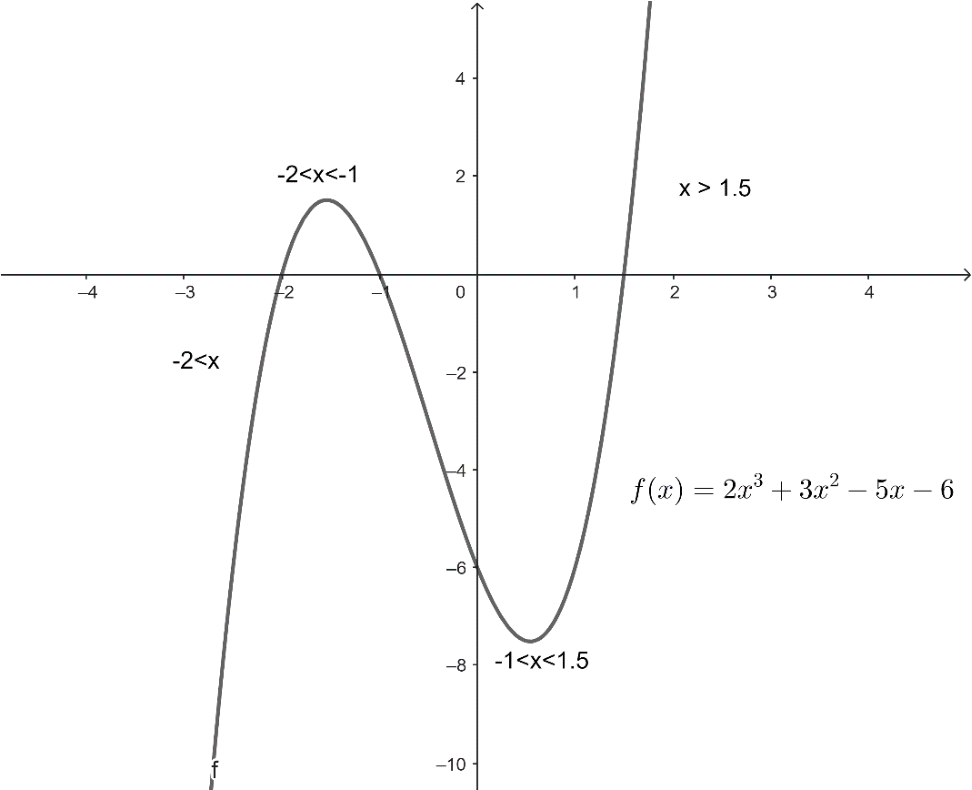
\includegraphics[width=0.75\linewidth]{figures/fig3-3.png}
\end{center}
\figcaption{3.3}{Curve of $2x^3 + 3x^2 - 5x - 6$}
\end{example}

\begin{example}{Example 3.7}
Sketch the curve $x^3 - 6x^2 + 5x + 12$

\solution
\textbf{Step 1:} a is 1 which is greater than 0. This means we know the shape the curve
will take.

\textbf{Step 2:} Using the factor theorem, the factors of the constant, 12 are
$\pm 1, \pm 2, \pm 3, \pm 4 \pm 6, \pm 12$

Testing when x $=$ - 1, we have:

$(-1)^3 - 6(-1)^2 + 5(-1) + 12$

$-1 - 6 - 5 + 12 = 0$

Which means $(x + 1)$ is a factor

We can use long division to find the other factors.
\[
\begin{array}{r@{\;}r}
 & x^2 - 7x + 12 \\ \cline{2-2}
x + 1\,\big) & x^3 - 6x^2 + 5x + 12 \\
 & \underline{-(x^3 + x^2 + 0 + 0)} \\
 & -7x^2 + 5x + 12 \\
 & (-7x^2 - 7x + 12) \\
 & 12x + 12 \\
 & \underline{-(12x + 12)} \\
 & 0
\end{array}
\]
\booknote[S3-07]{the line being subtracted is printed as $(-7x^2 - 7x + 12)$,
without the minus sign; it should be $-(-7x^2 - 7x + 0)$. The remainder line
$12x + 12$ and the quotient are correct.}

Factorising:

$x^2 - 7x + 12$

$x^2 - 4x - 3x + 12$

$x(x - 4) - 3(x - 4)$

$(x - 3)(x - 4)$

Factors are

$(x + 1)(x - 3)(x - 4)$

The zeros

$(x + 1)(x - 3)(x - 4) = 0$

$x = -1$, $x = 3$, $x = 4$

\textbf{Step 3:} $y$ intercept

At x $=$ 0

$(0)^3 - 6(0)^2 + 5(0) + 12 = 12$

\textbf{Step 4}: finding the intervals using the zeros
\begin{center}
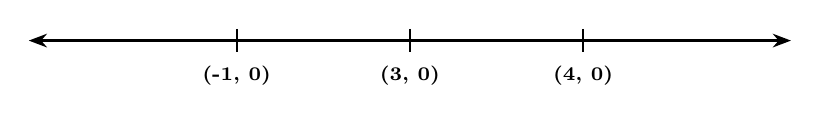
\begin{tikzpicture}[x=2.2cm]
  \draw[{Stealth}-{Stealth}, thick] (-0.7,0) -- (3.7,0);
  \foreach \x/\l in {0.5/{(-1, 0)}, 1.5/{(3, 0)}, 2.5/{(4, 0)}} {
    \draw[thick] (\x,0.15) -- (\x,-0.15);
    \node[below, font=\scriptsize\bfseries] at (\x,-0.2) {\l};
  }
\end{tikzpicture}
\end{center}
The interval are
\begin{enumerate}
  \item $-1 < x$
  \item $-1 < x < 3$
  \item $3 < x < 4$
  \item $x > 4$
\end{enumerate}
\booknote[S3-06]{see the note at Example 3.6: the first interval should be $x < -1$.}

Next is to determine the signs or test for the signs in each of the intervals obtained

\noindent\textbf{Table 3.1:} Test for signs in each of the intervals obtained
\begin{center}
\small\renewcommand{\arraystretch}{1.2}
\begin{tabular}{|p{0.2\linewidth}|p{0.15\linewidth}|p{0.15\linewidth}|p{0.15\linewidth}|p{0.15\linewidth}|}
\hline
\textbf{Interval} & {\boldmath$-2 > x$} & {\boldmath$-2 < x < -1$} & {\boldmath$-1 < x < 1.5$} & {\boldmath$x > 1.5$} \\
\hline
Chosen values (you can choose any number within the interval)
& \centering\textbf{-2} & \centering\textbf{1} & \centering\textbf{3.5} & \centering\textbf{5} \tabularnewline
\hline
y value (substitute your chosen number into the given function)
& \centering $(-2)^3 - 6(-2)^2 + 5(-2) + 12$ \par\medskip \textbf{= -30}
& \centering $(1)^3 - 6(1)^2 + 5(1) + 12$ \par\medskip \textbf{= 12}
& \centering $(3.5)^3 - 6(3.5)^2 + 5(3.5) + 12$ \par\medskip \textbf{= -1.125}
& \centering $2(5)^3 + 3(5)^2 - 5(5) - 6$ \par\medskip \textbf{= 294} \tabularnewline
\hline
Sign & \centering Negative & \centering Positive & \centering Negative & \centering Positive \tabularnewline
\hline
Behaviour of curve & Below x - axis & Above x - axis & Below x - axis & Above x - axis \\
\hline
\end{tabular}
\end{center}
\booknote[S3-08]{Table 3.1 repeats the interval headings of Example 3.6
($-2 > x$, $-2 < x < -1$, $-1 < x < 1.5$, $x > 1.5$) instead of $x < -1$,
$-1 < x < 3$, $3 < x < 4$, $x > 4$, and the last column evaluates the Example 3.6
polynomial $2x^3 + 3x^2 - 5x - 6$ at $x = 5$ (giving 294) instead of
$x^3 - 6x^2 + 5x + 12$, which gives 12. The sign, Positive, is unchanged.}

\begin{center}
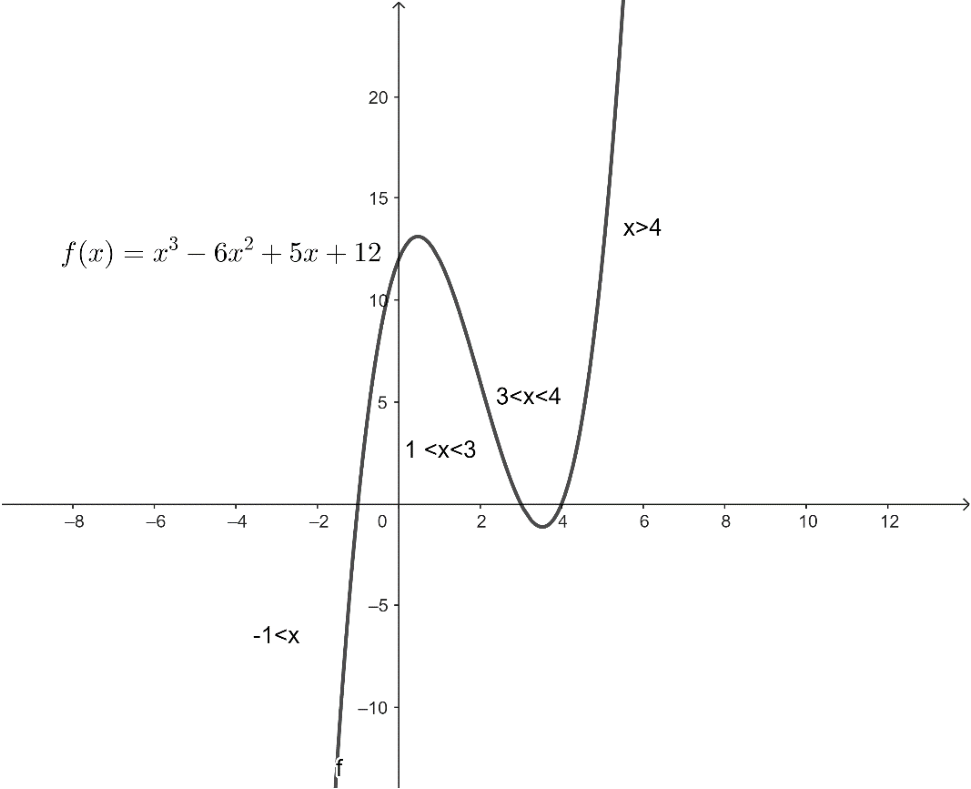
\includegraphics[width=0.75\linewidth]{figures/fig3-4.png}
\end{center}
\figcaption{3.4}{Curve of $x^3 - 6x^2 + 5x + 12$}
\end{example}

\begin{example}{Example 3.8}
Sketch the curve $-x^3 + 4x^2 - x - 6$

\solution
\textbf{Step 1:} a is -1 which is less than 0. This means that the extremes of the graph
go from top left to bottom right.

\textbf{Step 2:} Using the factor theorem, the factors of the constant, -6 are
$\pm 1, \pm 2, \pm 3, \pm 6$

Testing when x $=$ 2, we have:

$-(2)^3 + 4(2)^2 - 2 - 6 = -8 + 16 - 2 - 6 = 0$

Which means $(x - 2)$ is a factor.

We can use long division to find the other factors.
\[
\begin{array}{r@{\;}r}
 & -x^2 + 2x + 3 \\ \cline{2-2}
x - 2\,\big) & -x^3 + 4x^2 - x - 6 \\
 & \underline{-(-x^3 + 2x^2 + 0 + 0)} \\
 & 2x^2 - x - 6 \\
 & -(2x^2 - 4x - 6) \\
 & 3x - 6 \\
 & \underline{-(3x - 6)} \\
 & 0
\end{array}
\]
\booknote[S3-09]{the second subtraction is printed as $-(2x^2 - 4x - 6)$; the
line being subtracted is $2x(x - 2) = 2x^2 - 4x + 0$. The remainder $3x - 6$
and the quotient are correct.}

Factorising:

$-x^2 + 2x + 3$

$-x^2 + 3x - x + 3$

$-x(x - 3) - 1(x - 3)$

$(-x - 1)(x - 3)$

Factors are

$(x - 2)(x - 3)(-x - 1)$

The zeros

$(x - 2)(x - 3)(-x - 1) = 0$

$x = -1$, $x = 3$, $x = 2$

\textbf{Step 3:} y intercept:

When x $=$ 0

$-(0)^3 + 4(0)^2 - (0) - 6 = -6$

\textbf{Step 4}: finding the intervals using the zeros
\begin{center}
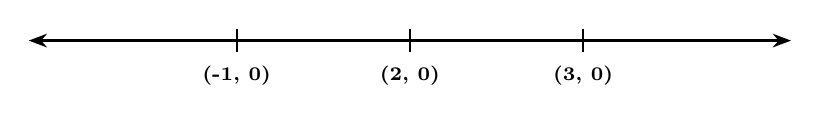
\begin{tikzpicture}[x=2.2cm]
  \draw[{Stealth}-{Stealth}, thick] (-0.7,0) -- (3.7,0);
  \foreach \x/\l in {0.5/{(-1, 0)}, 1.5/{(2, 0)}, 2.5/{(3, 0)}} {
    \draw[thick] (\x,0.15) -- (\x,-0.15);
    \node[below, font=\scriptsize\bfseries] at (\x,-0.2) {\l};
  }
\end{tikzpicture}
\end{center}
The intervals are
\begin{enumerate}
  \item $-1 < x$
  \item $-1 < x < 2$
  \item $2 < x < 3$
  \item $x > 3$
\end{enumerate}
\booknote[S3-06]{see the note at Example 3.6: the first interval should be $x < -1$.}

Next is to determine the signs or test for the signs in each of the intervals obtained

\noindent\textbf{Table 3.2:} Test for signs in each of the intervals obtained
\begin{center}
\small\renewcommand{\arraystretch}{1.2}
\begin{tabular}{|p{0.2\linewidth}|p{0.15\linewidth}|p{0.15\linewidth}|p{0.15\linewidth}|p{0.15\linewidth}|}
\hline
\textbf{Interval} & {\boldmath$-1 > x$} & {\boldmath$-1 < x < 2$} & {\boldmath$2 < x < 3$} & {\boldmath$x > 3$} \\
\hline
Chosen values (you can choose any number within the interval)
& \centering\textbf{-3} & \centering\textbf{1} & \centering\textbf{2.5} & \centering\textbf{4} \tabularnewline
\hline
y value (substitute your chosen number into the given function)
& \centering $-(-3)^3 + 4(-3)^2 - (-3) - 6$ \par\medskip \textbf{= 60}
& \centering $-(1)^3 + 4(1)^2 - (1) - 6$ \par\medskip \textbf{= -4}
& \centering $-(2.5)^3 + 4(2.5)^2 - (2.5) - 6$ \par\medskip \textbf{= 0.875}
& \centering $-(4)^3 + 4(4)^2 - (4) - 6$ \par\medskip \textbf{= -10} \tabularnewline
\hline
Sign & \centering Positive & \centering Negative & \centering Positive & \centering Negative \tabularnewline
\hline
Behaviour of curve & Above $x$ - axis & Below $x$ - axis & Above $x$ - axis & Below $x$ - axis \\
\hline
\end{tabular}
\end{center}

\begin{center}
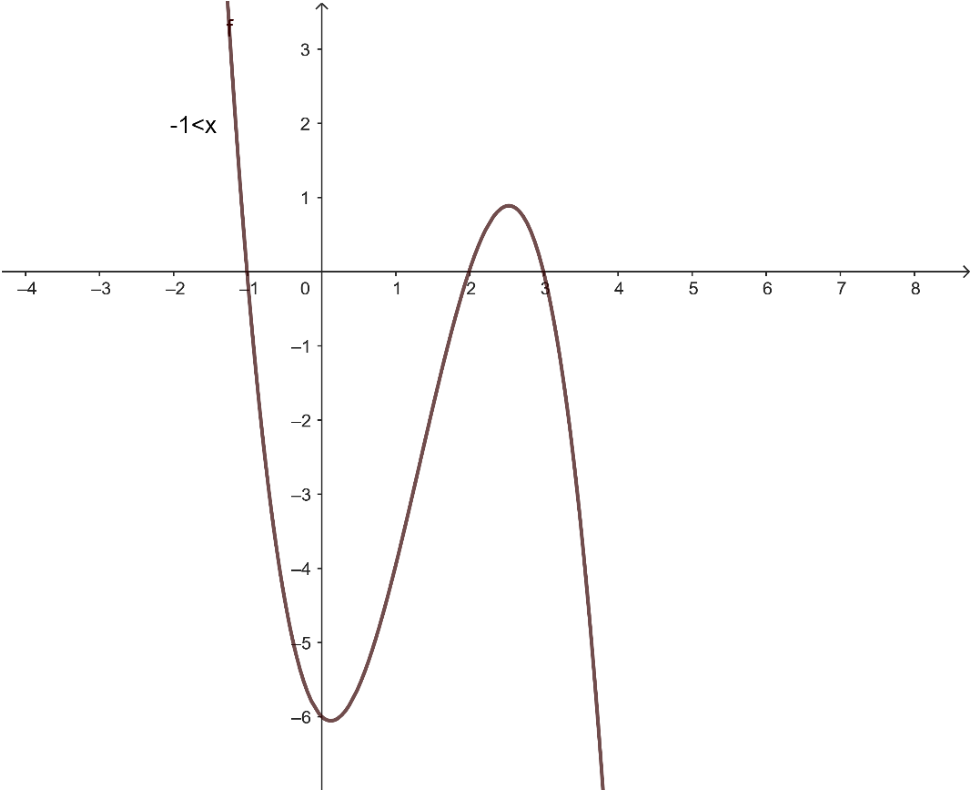
\includegraphics[width=0.75\linewidth]{figures/fig3-5.png}
\end{center}
\figcaption{3.5}{\textit{Curve of} $-x^3 + 4x^2 - x - 6$}
\end{example}

What polynomial function is represented in the graph below?
\begin{enumerate}
  \item[a.] How many factors does it have?
  \item[b.] Share your answers with the class.
\end{enumerate}
\begin{center}
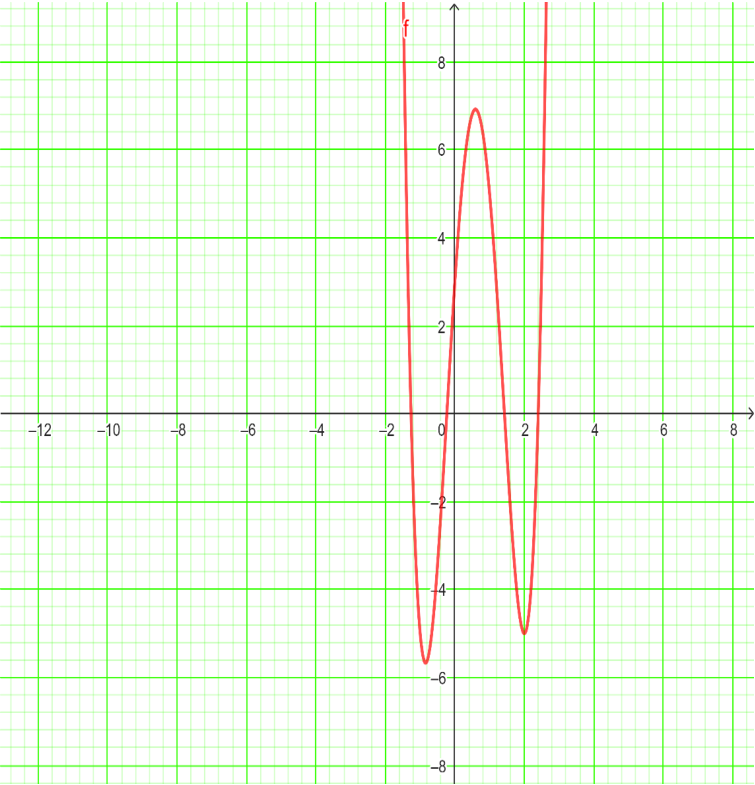
\includegraphics[width=0.6\linewidth]{figures/fig3-6.png}
\end{center}
\figcaption{3.6}{Graph of a polynomial function}

Remember that it is an important skill to be able to sketch graphs by hand.
However, when appropriate technology is there to assist. For example, you can
use apps or web-based programs such as GeoGebra, Demos, PhET Simulations
and Geometer's Sketch Pad.

% Book pp. 111-116 (PDF pp. 112-117)
\section{Applying Descartes' Rule of Signs Theorem}

There is another way that can be used to determine how many positive and negative
real zeros a polynomial function might have. To do this, first write the polynomial
in descending order (from the highest degree to the lowest) if it is not already. We
use \textbf{Descartes' Rule of Signs}. This rule helps you see how the number of times
the signs change in the polynomial is related to the number of positive real zeros.

For example, if you look at the polynomial function below, you will notice it has
one sign change, which gives you information about its positive zeros.

Let us go through an example using Descartes' Rule of Signs to determine the
possible number of positive and negative real zeros.

\begin{example}{Example 3.9}
Consider the polynomial:

$f(x) = 3x^3 - 2x^2 + 4x - 5$

\solution
\textbf{Step 1:} \textit{Identify Sign Changes for Positive Real Zeros}
\begin{enumerate}
  \item Write the polynomial in descending order:
  \item $f(x) = 3x^3 - 2x^2 + 4x + 5$
  \booknote[S3-10]{the polynomial is $3x^3 - 2x^2 + 4x - 5$, as in the question
  and in the coefficient list that follows; the ``$+ 5$'' is a misprint.}

  Look at the coefficients:

  3 (positive)

  --2 (negative)

  4 (positive)

  $-5$ (negative)
  \item Determine the sign changes:

  From 3 to -2 (1 change)

  From $-2$ to 4 (2 changes)

  From 4 to $-5$ (3 changes)

  Total sign changes for positive zeros $=$ 3. This means there could be 3,
  (3 -- 2 $=$ 1) positive real zeros. Note, the number of possible roots is found by
  subtracting 2 each time until we would get a negative number.
\end{enumerate}
\textbf{Step 2:} \textit{Identify Sign Changes for Negative Real Zeros}
\begin{quote}
Now, let's find the negative real zeros by evaluating f($-x$):

$f(-x) = 3(-x)^3 - 2(-x)^2 + 4(-x) - 5$

$f(-x) = -3x^3 - 2x^2 - 4x - 5$
\end{quote}
\textbf{Step 3:} \textit{Look at the Signs of f($-x$)}
\begin{quote}
The coefficients are:

$-3$ (negative)

$-2$ (negative)

$-4$ (negative)

$-5$ (negative)
\end{quote}
\textbf{Step 4:} \textit{Determine Sign Changes for Negative Real Zeros}
\begin{quote}
There are \textbf{no sign changes} in f($-$x)
\end{quote}
Total sign changes for negative zeros $=$ 0. This means there are no negative real
roots or zeros.
\end{example}

This example illustrates how to use Descartes' Rule of Signs to analyse a polynomial
and determine the possible numbers of positive and negative real zeros.

Let us solve more examples.

\begin{example}{Example 3.10}
Use Descartes' Rule of Signs to determine how many possible positive and
negative real zeros of the following:
\begin{enumerate}
  \item[a.] $g(x) = 2x^4 - 11x^3 + 4x^2 - 8x - 40$
  \item[b.] $g(x) = 9x^3 - 10x^2 + 5x + 3$
  \item[c.] f$(x) = -x^5 + 3x^4 - 5x^3 - 12x^2 + 6x + 4$
\end{enumerate}

\solution
\begin{enumerate}
  \item[a.] $g(x) = 2x^4 - 11x^3 + 4x^2 - 8x - 40$
\end{enumerate}
\textbf{Step 1:} \textit{Identify Sign Changes for Positive Real Zeros}
\begin{quote}
Write the polynomial in descending order:

$g(x) = 2x^4 - 11x^3 + 4x^2 - 8x - 40$

Look at the coefficients:

2 (positive)

--11 (negative)

4 (positive)

$-8$ (negative)

$-40$ (negative)

Look at the coefficients:

Determine the sign changes:

From 2 to -11 (1 change)

From $-11$ to 4 (2 changes)

From 4 to $-8$ (3 changes)

From -8 to $-40$ (no change)

Total sign changes for positive zeros $=$ 3. This means there could be 3 or 1
positive real zeros.
\end{quote}
\textbf{Step 2:} \textit{Identify Sign Changes for Negative Real Zeros}
\begin{quote}
Now, let's find the negative real zeros by evaluating f($-$x):

$g(x) = 2(-x)^4 - 11(-x)^3 + 4(-x)^2 - 8(-x) - 40$

$g(x) = 2x^4 + 11x^3 + 4x^2 + 8x - 40$
\end{quote}
\textbf{Step 3:} \textit{Look at the Signs of f($-x$)}
\begin{quote}
The coefficients are:

2 (positive)

11 (positive)

4 (positive)

8 (positive)

$-40$ (negative)
\end{quote}
\textbf{Step 4:} \textit{Determine Sign Changes for Negative Real Zeros}
\begin{quote}
Determine the sign changes:

From 2 to 11 (no change)

From 11 to 4 (no changes)

From 4 to 8 (no changes)

From 8 to $-40$ (1 change)

Total sign changes for negative zeros $=$ 1. This means there is 1 negative
real zero.
\end{quote}
\begin{enumerate}
  \item[b.] $g(x) = 9x^3 - 10x^2 + 5x + 3$
\end{enumerate}
\textbf{Step 1:} \textit{Identify Sign Changes for Positive Real Zeros}
\begin{quote}
Write the polynomial in descending order: $g(x) = 9x^3 - 10x^2 + 5x + 3$.

Look at the coefficients:

9 (positive)

$-10$ (negative)

5 (positive)

3 (negative)
\booknote[S3-11]{3 is positive; the sign changes counted below (2) are right.}

Determine the sign changes:

From 9 to -10 (1 change)

From $-10$ to 5 (2 changes)

From 5 to 3 (no change)

Total sign changes for positive zeros $=$ 2. This means there could be 2 or 0.
\end{quote}
\textbf{Step 2:} \textit{Identify Sign Changes for Negative Real Zeros}
\begin{quote}
Now, let's find the negative real zeros by evaluating g($-$x):

$g(x) = 9(-x)^3 - 10(-x)^2 + 5(-x) + 3$

$g(x) = -9x^3 - 10x^2 - 5x + 3$
\end{quote}
\textbf{Step 3:} \textit{Look at the Signs of f($-x$)}
\begin{quote}
The coefficients are:

$-9$ (negative)

$-10$ (negative)

$-5$ (negative)

3 (positive)
\end{quote}
\textbf{Step 4:} \textit{Determine Sign Changes for Negative Real Zeros}
\begin{quote}
Determine the sign changes:

From -9 to -10 (no change)

From -10 to -5 (no changes)

From -5 to 3 (1 change)

Total sign changes for negative zeros $=$ 1. This means there is 1 negative
real zero.
\end{quote}
\begin{enumerate}
  \item[c.] f$(x) = -x^5 + 3x^4 - 5x^3 - 12x^2 + 6x + 4$
\end{enumerate}
\textbf{Step 1:} \textit{Identify Sign Changes for Positive Real Zeros}
\begin{quote}
Write the polynomial in descending order:

f$(x) = -x^5 + 3x^4 - 5x^3 - 12x^2 + 6x + 4$

Look at the coefficients:

$-1$ (negative)

3 (positive)

$-5$ (negative)

$-12$ (negative)

6 (positive)

4 (positive)

\textit{Determine the sign changes:}

From $-1$ to 3 (1 change)

From 3 to $-5$ (2 changes)

\textbf{From $-5$ to $-12$ (no changes)}

From $-12$ to 6 (3 changes)

From 6 to 4 (no change)

Total sign changes for positive zeros $=$ 3. This means there could be 3 or 1
positive real zeros.
\end{quote}
\textbf{Step 2:} \textit{Identify Sign Changes for Negative Real Zeros}
\begin{quote}
Now, let's find the negative real zeros by evaluating f($-$x):

f$(x) = -(-x)^5 + 3(-x)^4 - 5(-x)^3 - 12(-x)^2 + 6(-x) + 4$

f$(x) = x^5 + 3x^4 + 5x^3 - 12x^2 - 6x + 4$
\end{quote}
\textbf{Step 3:} Look at the Signs of f($-$x)
\begin{quote}
The coefficients are:

1 (positive)

3 (positive)

5 (positive)

--12 (negative)

--6 (negative)

4 (positive)
\end{quote}
\textbf{Step 4:} \textit{Determine Sign Changes for Negative Real Zeros}
\begin{quote}
Determine the sign changes:

From 1 to 3 (no change)

From 3 to 5 (no changes)

From 5 to $-12$ (2 changes)

From $-2$ to $-6$ no changes)
\booknote[S3-12]{``From $-2$'' should read ``From $-12$''; and the count of changes
in the line above (2) should be 1, the line below 2, giving the printed total of 2.}

From $-6$ to 4 (3 change)

Total sign changes for negative zeros $=$ 2. This means there is 2 or 0 negative
real zeros.
\end{quote}
\end{example}

% Book pp. 116-122 (PDF pp. 117-123)
\section{Applying the Fundamental Theorem of Algebra}

The \textbf{Fundamental Theorem of Algebra} tells us something very important about
polynomial functions. It says: `Every polynomial function of degree $n$ (where $n >
0$) has at least one complex zero.'

This might sound complicated at first, but here is what it means:
\begin{enumerate}
  \item The degree of a polynomial is the highest power of $x$ in the expression.
  \item For example, $x^3 - 2x^2 + 4x - 8$ has a degree of 3.
  \item Complex numbers include real numbers and imaginary numbers (numbers
  with $i$, where $i = \sqrt{-1}$)
  \item In factorising the polynomial, each root c$_i$ corresponds to a linear factor of
  the form $(x - c_i)$. This means we can write the polynomial as f(x) $= a\,(x -
  c_1)\,(x - c_2) \cdots (x - c_n)$.

  The, $a$ is a non-zero number that affects how the polynomial behaves, and
  $c_1, c_2, \ldots, c_n$, are the roots, or zeros.
\end{enumerate}
Let us go through these examples to show how it works.

\begin{example}{Example 3.11}
Factorise the polynomial f$(x) = 3x^5 - 48x$ completely and find all its zeros.

State the multiplicity of each zero.

\solution
f$(x) = 3x^5 - 48x$

Factorising:

$3x(x^4 - 16)$

$3x[(x^2)^2 - 4^2]$

$3x[(x^2 + 4)(x^2 - 4)]$

$3x[x^2 - (-4)(x^2 - 4)]$

$3x[(x + 2i)(x - 2i)(x + 2)(x - 2)]$

To find the zeros, equate the factors to zero:

$3x[(x + 2i)(x - 2i)(x + 2)(x - 2)] = 0$

$3x = 0$, $x = 0$

$x + 2i = 0$, $x = -2i$

$x - 2i = 0$, $x = 2i$

$x + 2 = 0$, $x = -2$

$x - 2 = 0$, $x = 2$

Therefore, the zeros of f($x$) are 0, 2, -- 2, 2$i$ and -- 2$i$. Since each factor occurs
only once, all the zeros are of multiplicity 1 and the total number of zeros is five.
\end{example}

\begin{example}{Example 3.12}
Factorise the polynomial f$(x) = x^4 - 625$ completely and find all its zeros.

State the multiplicity of each zero.

\solution
f$(x) = x^4 - 625$

Factorising:

$(x^4 - 625)$

$[(x^2)^2 - 25^2]$

$[(x^2 + 25)(x^2 - 25)]$

$3x[x^2 - (-25)(x^2 - 25)]$
\booknote[S3-13]{the ``$3x$'' is carried over from Example 3.11; there is no such
factor here.}

$[(x + 5i)(x - 5i)(x + 5)(x - 5)]$

To find the zeros, equate the factors to zero:

$[(x + 5i)(x - 5i)(x + 5)(x - 5)] = 0$

$x + 5i = 0$, $x = -5i$

$x - 5i = 0$, $x = 5i$

$x + 5 = 0$, $x = -5$

$x - 5 = 0$, $x = 5$

Therefore, the zeros of f($x$) are 5, -- 5, 5$i$ and -- 5$i$. Since each factor occurs
only once, all the zeros are of multiplicity 1 and the total number of zeros is four.
\end{example}

\begin{example}{Example 3.13}
Factorise the polynomial f$(x) = 15x^4 + 8x^2 + 1$ completely and find all its zeros.

State the multiplicity of each zero.

\solution
f$(x) = 15x^4 + 8x^2 + 1$

in this scenario, we can represent $x^2$ by any other letter, for example, u

$f(x) = 15(x^2)^2 + 8x^2 + 1$

$f(x) = 15(u)^2 + 8u + 1$

$15u^2 + 8u + 1$

Factorising:

$15u^2 + 5u + 3u + 1$

$5u(3u + 1) + (3u + 1)$

$(5u + 1)(3u + 1)$

Substituting $x^2$ back,

$(5x^2 + 1)(3x^2 + 1)$

To find the zeros, equate the factors to zero:

$(5x^2 + 1)(3x^2 + 1) = 0$

$5x^2 + 1 = 0$ or $3x^2 + 1 = 0$

For $5x^2 + 1 = 0$

$5x^2 = -1$

$x^2 = -\frac{1}{5}$

$x = \pm\sqrt{-\frac{1}{5}}$

$x = -\sqrt{-\frac{1}{5}}$ or $x = \sqrt{-\frac{1}{5}}$

For $x = -\sqrt{-\frac{1}{5}}$

$x = -\sqrt{\frac{1}{5}} \times \sqrt{-1}$

$x = -i\sqrt{\frac{1}{5}}$

$x = -\frac{\sqrt{5}}{5}\,i$

For $x = \sqrt{-\frac{1}{5}}$

$x = \sqrt{\frac{1}{5}} \times \sqrt{-1}$

$x = i\sqrt{\frac{1}{5}}$

$x = \frac{\sqrt{5}}{5}\,i$

For $3x^2 + 1 = 0$

$3x^2 = -1$

$x^2 = -\frac{1}{3}$

$x = \pm\sqrt{-\frac{1}{3}}$

$x = -\sqrt{-\frac{1}{3}}$ or $x = \sqrt{-\frac{1}{3}}$

For $x = -\sqrt{-\frac{1}{3}}$

$x = -\sqrt{\frac{1}{3}} \times \sqrt{-1}$

$x = -i\sqrt{\frac{1}{3}}$

$x = -\frac{\sqrt{3}}{3}\,i$

For $x = \sqrt{-\frac{1}{3}}$

$x = \sqrt{\frac{1}{3}} \times \sqrt{-1}$

$x = i\sqrt{\frac{1}{3}}$

$x = \frac{\sqrt{3}}{3}\,i$

Therefore, the zeros of $f(x)$ $\frac{\sqrt{3}}{3}\,i, -\frac{\sqrt{3}}{3}\,i,
-\frac{\sqrt{5}}{5}\,i, \frac{\sqrt{5}}{5}\,i$. Since each factor occurs only once, all
the zeros are of multiplicity 1 and the total number of zeros is four.
\end{example}

\begin{example}{Example 3.14}
Factorise the polynomial f$(x) = x^4 - 4x^2 - 21$ completely and find all its zeros.

State the multiplicity of each zero.

\solution
f$(x) = x^4 - 4x^2 - 21$

in this scenario, we can represent $x^2$ by u

$f(x) = (x^2)^2 - 4x^2 - 21$

$f(x) = (u)^2 - 4u - 21$

$u^2 - 4u - 21$

Factorising:

$u^2 - 7u + 3u - 21$

$u(u - 7) + 3(u - 7)$

$(u + 3)(u - 7)$

Substituting $x^2$ back,

$(x^2 + 3)(x^2 - 7)$

To find the zeros, equate the factors to zero:

$(x^2 + 3)(x^2 - 7) = 0$

$x^2 + 3 = 0$ or $x^2 - 7 = 0$

For $x^2 + 3 = 0$

$x^2 = -3$

$x^2 = -3$

$x = \pm\sqrt{-3}$

$x = -\sqrt{-3}$ or $x = \sqrt{-3}$

For $x = -\sqrt{-3}$

$\sqrt{-3} = -\sqrt{3} \times \sqrt{-1}$

$x = -\sqrt{3} \times \sqrt{-1}$

$x = -i\sqrt{3}$

For $x = \sqrt{-3}$

$x = \sqrt{3} \times \sqrt{-1}$

$x = i\sqrt{3}$

For $x^2 - 7$

$x^2 = 7$

$x^2 = 7$

$x = \pm\sqrt{7}$

$x = -\sqrt{7}$ or $x = \sqrt{7}$

For $x = -\sqrt{7}$

$x = -\sqrt{7}$

For $x = \sqrt{7}$

$x = \sqrt{7}$

$x = \sqrt{7}$

Therefore, the zeros of $f(x)$ are $x = i\sqrt{3}$, $x = -i\sqrt{3}$, $x = -\sqrt{7}$,
$x = \sqrt{7}$. Since each factor occurs only once, all the zeros are of multiplicity
1 and the total number of zeros is four.
\end{example}

Note: Multiplicity refers to the number of times a particular zero (or root) appears
in the factorisation of a polynomial. It indicates how many times a specific value
$x = r$ is a solution to the polynomial equation P($x$) $=$ 0.

\noindent\textit{\color{blue}Key Points about Multiplicity:}
\begin{enumerate}
  \item Simple Roots: If a root appears once, it has a multiplicity of 1. For example,
  in the polynomial $(x - 2)$, the root $x = 2$ has multiplicity 1.
  \item Repeated Roots: If a root appears more than once, it has a higher multiplicity.
  For example, in the polynomial $(x - 2)^2$, the root $x = 2$ has a multiplicity of
  2.
  \item Multiplicity and Behaviour: This can be even or odd.
\end{enumerate}
\textit{Odd Multiplicity}: If a root has an odd multiplicity, the graph of the polynomial
crosses the $x$ - axis at that root.

\textit{Even Multiplicity}: If a root has an even multiplicity, the graph of the polynomial
touches the x-axis at that root but does not cross it.

For instance, for the polynomial P(x) $= (x - 1)\,(x - 1)\,(x + 2)$:

The root $x = 1$ has a multiplicity of 2 (it appears twice), so the graph just touches
the x-axis at x $=$ 1 and does not cross it.

The root $x = -2$ has a multiplicity of 1 (it appears once), so the graph crosses the
x-axis at x $=$ -2.

% Book pp. 122-125 (PDF pp. 123-126)
\section{Complex Conjugates Theorem}

\textbf{Complex Numbers}: A complex number is expressed in the form $a + bi$, where a
and b are real numbers, and $i$ is the imaginary unit defined as $i^2 = -1$, or
$i = \sqrt{-1}$

\textbf{Roots of Polynomials}: When dealing with polynomial equations, the Fundamental
Theorem of Algebra states that every non-constant polynomial has at least one
complex root. This means that if a polynomial has real coefficients, any non-real
roots must occur in conjugate pairs.

If $a + bi$ (where b $\ne$ 0) is a root of a polynomial, then its conjugate $a - bi$ is
also a root.

\textbf{Example}: For a polynomial like $x^2 + 4$:

The roots can be found by rearranging to $x^2 = -4$.

Taking the square root gives $x = \pm 2i$

Here, $2i$ and $-2i$ are complex roots that come in conjugate pairs.

\textbf{Note that:}

\textbf{Complex roots} always come in \textbf{conjugate pairs}.

If $a + bi$ is a root of a polynomial, then $a - bi$ is also a root.

This property helps us find all the roots of polynomials, ensuring we account for
both real and complex solutions.

The \textbf{Complex Conjugate Theorem} states that if a polynomial has a complex
root, its conjugate must also be a root. This is an important concept in algebra that
helps us understand the nature of polynomial equations and their solutions.

Let us go through the following examples to explore how to use the \textbf{Complex
conjugate theorem.}

For example, if we are given one complex factor of a polynomial, we know
another factor must be the complex conjugate. This gives us two factors. We can
then form a quadratic equation and use algebraic division to find another factor.
Or we may be given two real factors, for example, $x = 2$ and $x = -3$. This means
that $x - 2 = 0$ or $x + 3 = 0$

$\therefore (x - 2)(x + 3) = 0$

$x^2 + 3x - 2x - 6 = 0$

$x^2 + x - 6 = 0$

\begin{example}{Example 3.15}
Find all the roots of $f(x) = x^3 + 8x^2 + 21x + 20$ if one root is -2 $-$ $i$.

\solution
$f(x) = x^3 + 8x^2 + 21x + 20$

Since the factor given $(-2 - i)$ is complex in nature, we need the conjugate as
well: $-2 + i$

$[x - (-2 - i)][(x - (-2 + i)]$

$[x + 2 + i][x + 2 - i]$

$(x + 2)^2 - (i)^2$

$x^2 + 4x + 4 - i^2$

NB: $-i^2 = 1$

$x^2 + 4x + 4 - (-1)$

$x^2 + 4x + 5$

We can use long division to find the other factors:
\[
\begin{array}{r@{\;}r}
 & x + 4 \\ \cline{2-2}
x^2 + 4x + 5\,\big) & x^3 + 8x^2 + 21x + 20 \\
 & \underline{-(x^3 + 4x^2 + 5x + 20)} \\
 & 4x^2 + 16x + 20 \\
 & \underline{-(4x^2 + 16x + 20)} \\
 & 0
\end{array}
\]
$x + 4 = 0$

$x = -4$

Therefore, the roots of $(x)$ are $-4$, $-2 + i$ and $-2$ -- $i$
\end{example}

\begin{example}{Example 3.16}
Find all the roots of $f(x) = 2x^3 - 13x^2 + 26x - 10$ if one root is $3 + i$.

\solution
$f(x) = 2x^3 - 13x^2 + 26x - 10$

Since the factor given $3 + i$. is complex in nature, we need the conjugate as well:
$3 - i$

$[x - (3 + i)][(x - (3 - i)]$

$[x - 3 - i][x - 3 + i]$

$(x - 3)^2 - (i)^2$

$x^2 - 6x + 9 - i^2$

NB: $-i^2 = -1$
\booknote[S3-14]{$-i^2 = 1$, as Example 3.15 states; the next line correctly
subtracts $(-1)$.}

$x^2 - 6x + 9 - (-1)$

$x^2 - 6x + 10$

We can use long division to find the other factor.
\[
\begin{array}{r@{\;}r}
 & 2x - 1 \\ \cline{2-2}
x^2 - 6x + 10\,\big) & 2x^3 - 13x^2 + 26x - 10 \\
 & \underline{-(2x^3 - 12x^2 + 20x + 0)} \\
 & -x^2 + 6x - 10 \\
 & \underline{-(-x^2 + 6x - 10)} \\
 & 0
\end{array}
\]
$2x - 1 = 0$

$x = \frac{1}{2}$

Therefore, the roots of $(x)$ are $= \frac{1}{2}$, $3 + i$ and $3$ -- $i$
\end{example}

% Book pp. 125-128 (PDF pp. 126-129)
\section{Linear and Quadratic Factor Theorems}

The linear quadratic factor theorem is another method which can be used to solve
polynomial functions. This is when we break polynomial functions into linear and
quadratic factors to make solving it simpler.

For example, to use the linear and quadratic factor approach to find the factors of
$x^4 - 9x^2 + 14$, we:

\textbf{Step 1}: Let $x^2 = u$

\textbf{Step 2}: Using this substitution it means $x^4 - 9x^2 + 14 = (u)^2 - 9(u) + 14$

\textbf{Step 3}: Factorise $u^2 - 9u + 14$:

$u^2 - 7u - 2u + 14$

$u(u - 7) - 2(u - 7)$

$(u - 2)(u - 7)$

\textbf{Step 4}: Substitute $x^2$ back in for $u$:

$(x^2 - 2)(x^2 - 7)$

$x^2 - 2 = 0$ and $x^2 - 7 = 0$

For $x^2 - 2 = 0$

$x^2 = 2$

$x = \pm\sqrt{2}$

$x = -\sqrt{2}$ or $x = \sqrt{2}$

$x + \sqrt{2}$ and $x - \sqrt{2}$ are factors

For $x^2 - 7 = 0$

$x^2 = 7$

$x = \pm\sqrt{7}$

$x = -\sqrt{7}$ or $x = \sqrt{7}$

$x + \sqrt{7}$ and $x - \sqrt{7}$ are factors

Hence the factors are $+\sqrt{2}$, $x - \sqrt{2}$, $x + \sqrt{7}$ and $x - \sqrt{7}$

\begin{example}{Example 3.17}
Given $f(x) = x^4 - 1$, find all the factors using the linear quadratic factor approach.

\solution
Let $u = x^2$

$f(x) = (x^2)^2 - 1$

$(u)^2 - 1$

$u^2 - 1$

Factorising:

$(u - 1)(u + 1)$

Substituting $x^2$ back in:

$(x^2 - 1)(x^2 + 1)$

$(x^2 - 1)(x^2 + 1) = 0$

$x^2 - 1 = 0$ or $x^2 + 1 = 0$

For $x^2 - 1 = 0$

$x^2 = \pm 1$

$x = 1$ or $x = -1$

For $(x^2 + 1)$

$x^2 + 1 = 0$

$x^2 = -1$

$x = \pm\sqrt{-1}$

\textbf{NB:} $\sqrt{-1} = \boldsymbol{i}$

$x = \pm i$

$x = -i$ or $x = i$

Hence the factors are $(x + 1)$, $(x - 1)$, $(x - i)(x + i)$
\end{example}

\begin{example}{Example 3.18}
Given $f(x) = 2x^4 + x^2 - 10$, find all the factors using the linear quadratic factor
approach

\solution
Let $u = x^2$

$f(x) = 2(x^2)^2 + u - 10$

$2(u)^2 + u - 10$

$2u^2 + u - 10$

Factorising:

$2u^2 - 4u + 5u - 10$

$2u(u - 2) + 5(u - 2)$

$(2u + 5)(u - 2)$

Substituting:

$u = x^2$

$(2x^2 + 5)(x^2 - 2)$

$(2x^2 + 5)(x^2 - 2) = 0$

$2x^2 + 5 = 0$ or $x^2 - 2 = 0$

For $2x^2 + 5 = 0$

$x^2 = -\frac{5}{2}$

$x = \pm\sqrt{-\frac{5}{2}}$

$x = \frac{5}{2}\,i$ or $x = -\frac{5}{2}\,i$
\booknote[S3-15]{$\sqrt{-\frac{5}{2}} = \sqrt{\frac{5}{2}}\,i = \frac{\sqrt{10}}{2}\,i$,
not $\frac{5}{2}\,i$; the two complex factors in the last line inherit the slip.}

For $(x^2 - 2)$

$x^2 - 2 = 0$

$x^2 = 2$

$x = \pm\sqrt{2}$

$x = -\sqrt{2}$ or $x = \sqrt{2}$

Hence the factors are $\left(x + \frac{5}{2}\,i\right)\left(x - \frac{5}{2}\,i\right)
\left(x - \sqrt{2}\right)\left(x + \sqrt{2}\right)$
\end{example}

We can use what we have learned to help in determining the maximum or minimum
profit or productivity in the real world.

In small groups, or individually, discuss how the following problem can be solved.

\begin{example}{Example 3.19}
A water production company made sales of $x$ bags of water and the profit was
given by $2x^2 + 7x - 15$ where $0 \le x \le 10$.

Help the company determine their maximum profit and loss.

\solution
Since the range was given \textbf{(}$0 \le x \le 10$), we do our calculation within
this range.

Evaluating the function in the given interval, we obtain:
\begin{center}
\renewcommand{\arraystretch}{1.3}
\begin{tabular}{|l|c|c|c|c|c|c|c|c|c|c|c|}
\hline
x & 0 & 1 & 2 & 3 & 4 & 5 & 6 & 7 & 8 & 9 & 10 \\
\hline
$2x^2 + 7x - 15$ & -15 & -6 & 7 & 24 & 45 & 70 & 99 & 132 & 169 & 210 & 255 \\
\hline
\end{tabular}
\end{center}
The maximum profit occurs when x=10 with a profit of 255 while the loss will
occur when there is no production, i.e., $x = 0$ at a loss of 15 ( -15).
\end{example}

\section*{Extended Reading}
\begin{itemize}
  \item Lial, M. L., Hornsby, E. J., \& McGinnis, T. (2012). Algebra for college
  students. (7th Ed. Pearson Education, Inc). Pages 346 -- 375.
\end{itemize}

% Book pp. 129-132 (PDF pp. 130-133).  The numbering is the book's own.
\section*{Review Questions}

\begin{enumerate}
\item Use the Rational Zero Theorem to find the rational zeros of\textbf{:}
\begin{enumerate}
  \item[a.] $6x^3 - 13x^2 - 14x - 3$
  \item[b.] $5x^3 + 2x^2 - 5x - 2$
\end{enumerate}
\begin{center}
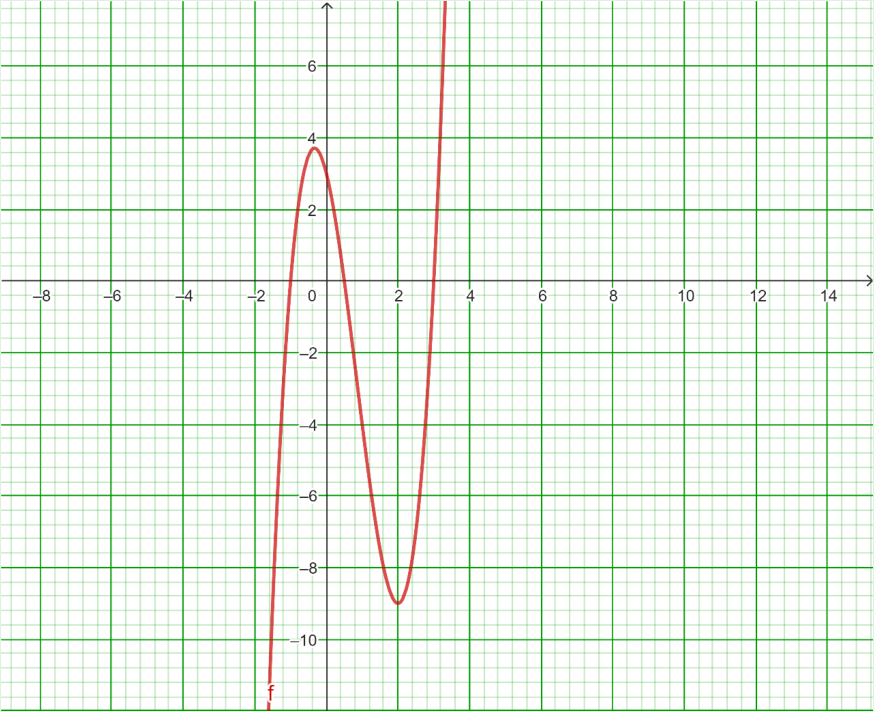
\includegraphics[width=0.7\linewidth]{figures/rq3-2.png}
\end{center}

\item Carefully, study the graph above which represents a polynomial function
f(x).
\begin{enumerate}
  \item[a.] State the zeros
  \item[b.] Find the factors
  \item[c.] State the interval on the curve.
  \item[d.] Find the polynomial function f(x)
\end{enumerate}

\item Sketch the following curves.
\begin{enumerate}
  \item[a.] $f(x) = x^3 + 2x^2 - 9x - 18$
  \item[b.] $f(x) = x^3 - 2x^2 - x + 2$
  \item[c.] $f(x) = x^3 + 3x^2 - 4x - 12$
  \item[d.] $f(x) = x^3 - 5x^2 - x + 5$
  \item[e.] $f(x) = \frac{1}{5}\left(x - 2\right)\left(x - 4\right)\left(x + 5\right)$
\end{enumerate}

\item Factorise:
\begin{enumerate}
  \item[a.] $x^3 + 5x^2 + 2x - 8$
  \item[b.] $2x^3 + 3x^2 - 17x - 30$
  \item[c.] $4x^3 - 4x^2 - 11x + 6$
  \item[d.] $6x^3 + 13x^2 - 4$
  \item[e.] $3x^3 + 16x^2 - 13x - 6$
\end{enumerate}

\item Find the zeros of the following:
\begin{enumerate}
  \item[a.] $x^3 + 4x^2 + x - 6$
  \item[b.] $2x^3 + 7x^2 - 14x + 5$
  \item[c.] $2x^3 + x^2 - 5x + 2$
  \item[d.] $4x^3 - 8x^2 - 9x + 18$
  \item[e.] $4x^3 - 4x^2 - x + 1$
  \item[f.] $4x^3 - 12x^2 + 11x - 3$
\end{enumerate}

\item Find the roots of:
\begin{enumerate}
  \item[a.] $x^3 + 6x$
  \item[b.] $2x^4 + 17x^2 + 35$
  \item[c.] $x^4 - 14x^2 + 36$
  \item[d.] $x^4 - 1$
  \item[e.] $x^3 + 27x$
\end{enumerate}
\begin{center}
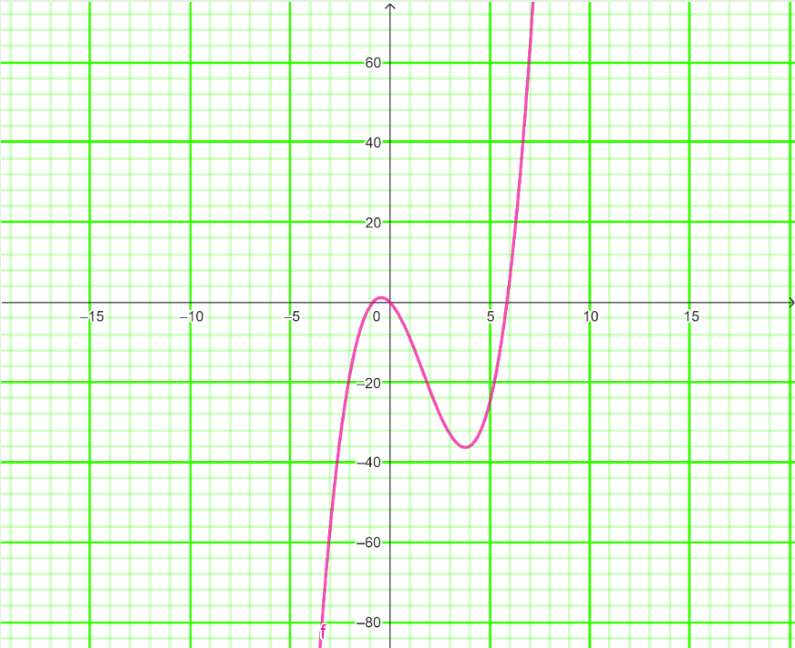
\includegraphics[width=0.65\linewidth]{figures/rq3-7.png}
\end{center}

\item Find the polynomial function f(x) as represented by the curve above.

\item $Q(x) = 10x^3 + ax^2 - 10x + b$, where $a$ and $b$ are integers, is divisible
by $(2x + 1)$. When $Q(x)$ is divided by $x + 1$, the remainder is -2.
\begin{enumerate}
  \item[a.] Find the values of a and of b
  \item[b.] find the expression for $Q(x)$ as a product of the three linear factors
\end{enumerate}

\item Given that $x_1 = 1 + \sqrt{2}\,i$ and $x_2 = 2 + 3i$ are roots of a polynomial
function $P(x)$, determine the $P(x) = 0$

\item Applying Descartes' Rule of Signs, identify the potential number of
positive and negative roots.
\begin{enumerate}
  \item[a.] $f(x) = 10x^6 - 5x^5 + 3x^4 - 6x^3 + 24x^2 - 38x$
  \item[b.] $f(x) = 19x^5 + 6x^4 + 17x^3 + 18x^2 - 38x - 70$
  \item[c.] $f(x) = x^6 - 729$
  \item[d.] $f(x) = 12x^6 + 13x^3 + 1$
  \item[e.] $f(x) = 8x^8 - 13x^4 + 100$
\end{enumerate}

\item Write down the equation having only the following roots.
\begin{enumerate}
  \item[a.] -5 , -1, 3
  \item[b.] $3, -\frac{1}{5}, -\frac{1}{3}$
  \item[c.] 2, -2, $2 + \sqrt{3}$, $2 - \sqrt{3}$
  \item[d.] 0, 1 $+$ 4i, 1- 4i
\end{enumerate}

\item Find the four roots of $y^4 + 3x^2 + 2$
\booknote[S3-16]{the polynomial mixes $y$ and $x$; the answer key treats it as
$y^4 + 3y^2 + 2$.}

\item Study the graph below and use it to answer the following questions:
\begin{enumerate}
  \item[a.] state the factors
  \item[b.] find the polynomial function
  \item[c.] how many turning points
  \item[d.] what is the relationship between the degree of the function and the
  number of turning points
\end{enumerate}
\begin{center}
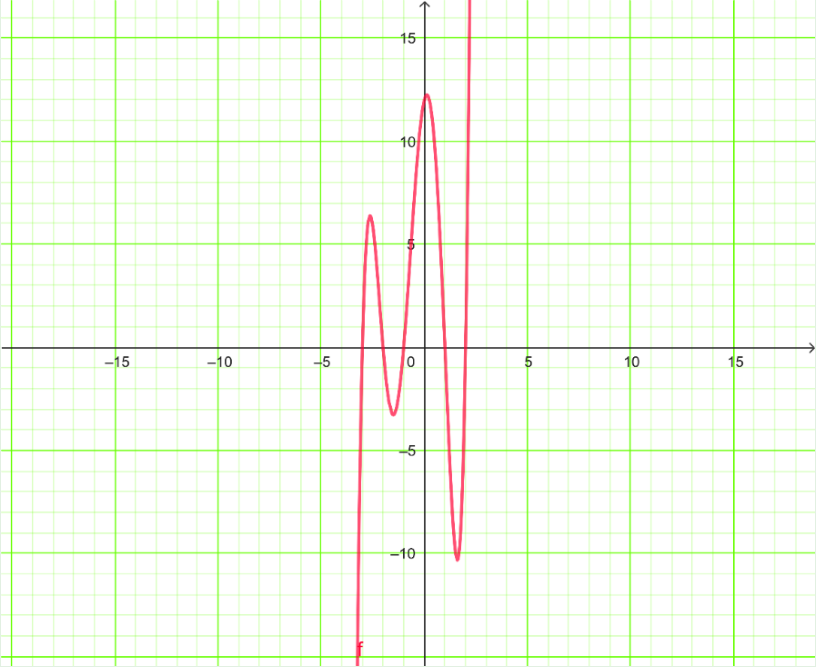
\includegraphics[width=0.65\linewidth]{figures/rq3-13.png}
\end{center}

\item A new bakery in Accra specialises in creating various types of bread. The
bakery wants the volume of a small rectangular loaf of bread to be 4 800
cm$^3$. The loaf is to be shaped like a rectangular solid. The length of the
loaf is to be 4cm longer than the width. The height of the loaf is one-half
of the width. Determine the dimensions of the loaf.
\end{enumerate}


\chapter{Circles and Loci}
% Book pp. 134-138 (PDF pp. 135-139)
\section*{Geometric Reasoning and Measurement}
\subsection*{Spatial Sense}

\section{Introduction}

In this section, you will learn how to derive the circle equation. You will also
learn how to manipulate this equation under given conditions and apply it to
solve real-life problems. The content of this section is imperative as it forms the
foundation on which other advanced topics in mathematics are built. Its real-life
applications are vast so why not delve further through your own research.

\begin{keyideas}
\begin{itemize}
  \item A circle is a path traced by all points in a plane which are equidistant
  from a fixed point in the plane. The fixed point is called the centre.
  \item The standard equation of a circle with centre $(h, k)$ and radius $r$ is given
  as:
  \item $(x - h)^2 + (y - k)^2 = r^2$
  \item The general equation of a circle with centre $(-g, -f)$ and radius $r$ is
  given as:
  \item $x^2 + y^2 + 2gx + 2fy + c = 0$
\end{itemize}
\end{keyideas}

\section{Exploring the Properties of a Circle and its Parts}

\subsection{A Circle}

The circle is the path traced by all points in a plane which are equidistant from a
fixed point in the plane. The fixed point is called the centre.

Let us use the activity below to revise the parts of the circle. You will need a
graph sheet and a set of mathematical instruments to do this activity.

\begin{activity}{Activity 4.1- Parts of a circle}
\textbf{Step 1:} Make a copy of the graph below.
\begin{center}
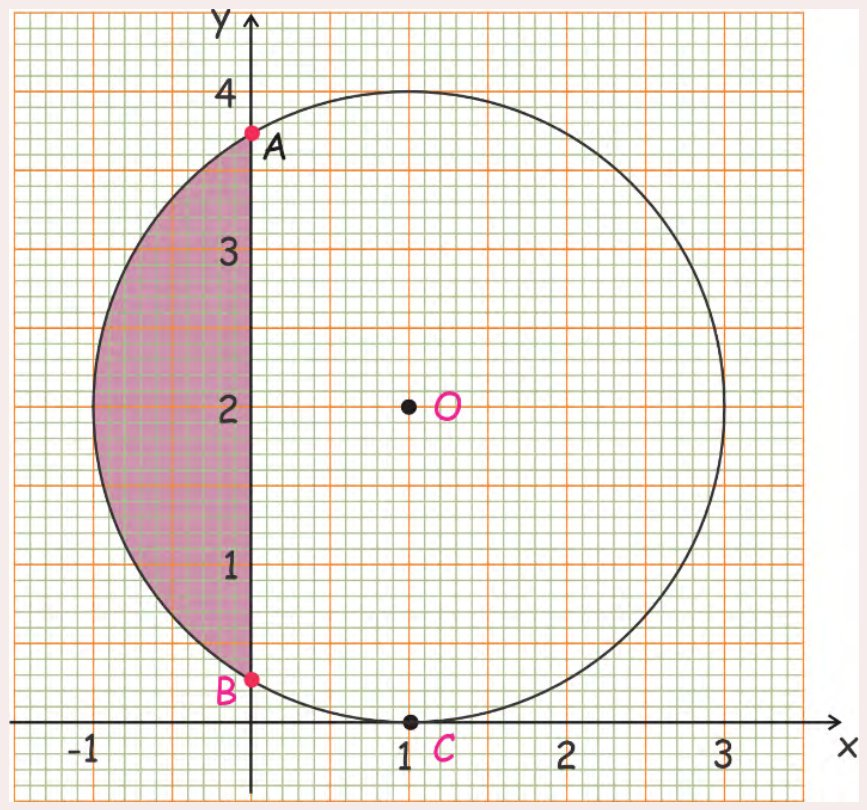
\includegraphics[width=0.6\linewidth]{figures/fig4-1.jpg}
\end{center}
\figcaption{4.1}{A circle}

\textbf{Step 2:} Calculate $|$OA$|$, $|$OB$|$ and $|$OC$|$

\textbf{Step 3:} Comment on any observation from your result in Step 2

\textbf{Step 4:} Aside from points A, B and C, list the coordinates of any two points
on the circle's circumference. Find the distance between these points and
point O. Comment on your observations.

\textbf{Step 5:} Join points O and C with a straight line.

Measure the angle between OC and the $x$-axis.
\end{activity}

\textbf{Let us use our diagram to revise the parts of the circle.}

Lines OA, OB and OC are the radii of the circle. From the activity, $|$OA$|=|$OB$|=|$OC$|$.

Line AB is an example of a chord. Any straight line that connects any two points
on the circumference of the circle is a chord.

\begin{center}
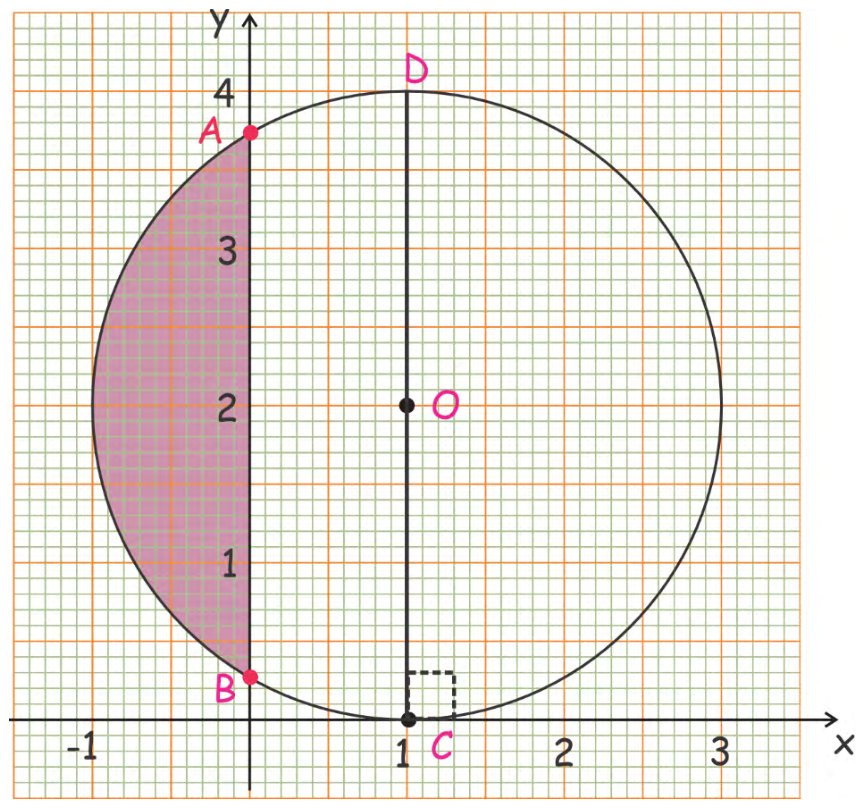
\includegraphics[width=0.6\linewidth]{figures/fig4-2.jpg}
\end{center}
\figcaption{4.2}{A circle}

The diameter is an example of a chord. It is the longest chord. The diameter is a
straight line from a point on the circumference through the centre to another point
on the circumference of the circle. In the above diagram, line COD is a diameter.

The $x$-axis is tangent to the circle at point C(1, 0). The tangent touches the circle
at one point. The angle between the tangent and the radius or the diameter at the
point of tangency is $90^\circ$. In the diagram OCX $= 90^\circ$

The area, shaded red, between the arc AB and the line AB is called a segment.

\begin{center}
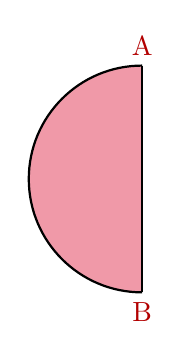
\begin{tikzpicture}[scale=0.9]
  \fill[red!40!purple!40] (0,-1.6) arc (270:90:1.6) -- cycle;
  \draw[black, thick] (0,-1.6) arc (270:90:1.6);
  \draw[black, thick] (0,1.6) -- (0,-1.6);
  \node[red!70!black, above] at (0,1.6) {A};
  \node[red!70!black, below] at (0,-1.6) {B};
\end{tikzpicture}
\end{center}
\figcaption{4.3}{A segment}

The area bounded by the arc AB and the lines OA and OB is called a sector.

\begin{center}
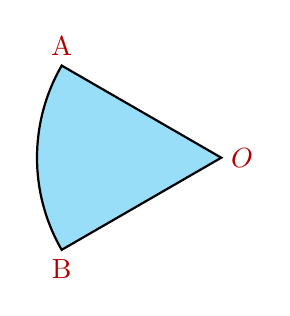
\begin{tikzpicture}[scale=0.9]
  \coordinate (O) at (0,0);
  \fill[cyan!40] (O) -- (150:2.6) arc (150:210:2.6) -- cycle;
  \draw[black, thick] (O) -- (150:2.6) arc (150:210:2.6) -- cycle;
  \node[red!70!black, right] at (O) {$O$};
  \node[red!70!black, above] at (150:2.6) {A};
  \node[red!70!black, below] at (210:2.6) {B};
\end{tikzpicture}
\end{center}
\figcaption{4.4}{A sector}

\begin{example}{Example 4.1}
The diagram below shows the graph of a circle. Use it to answer the questions.
\begin{center}
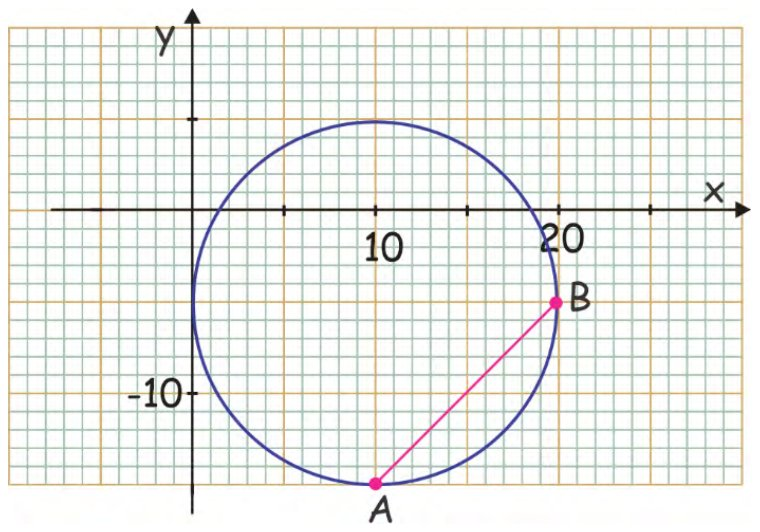
\includegraphics[width=0.55\linewidth]{figures/fig4-5.jpg}
\end{center}
\figcaption{4.5}{Graph of a circle}
\begin{enumerate}
  \item[a.] State the coordinates of the centre.
  \item[b.] Find the radius of the circle
  \item[c.] Find the length of chord AB
\end{enumerate}

\solution
\begin{enumerate}
  \item[a.] Coordinate of the centre is (10, -5)
  \item[b.] The radius of the circle is 10 units
  \item[c.] The coordinate of point A is (10, -15) and that of B is (20, -5)
  \item[d.] $|AB| = \sqrt{(20 - 10)^2 + (-5 \text{---} 15)^2}$
  \item[e.] $|AB| = \sqrt{10^2 + 10^2}$
  \item[f.] $= \sqrt{100 + 100}$
  \item[g.] $= \sqrt{200}$
  \item[h.] $= \sqrt{100 \times 2}$
  \item[i.] $= \sqrt{100} \times \sqrt{2}$
  \item[j.] $= 10\sqrt{2}$ units.
\end{enumerate}
\booknote[S4-01]{the working of part (c) is lettered d.\ to j.\ in the book as if
it were seven further parts; the question has only parts a--c.}
\booknote[S4-02]{the second bracket is printed ``$(-5\text{---}15)^2$''; it should
read $(-5 - (-15))^2 = 10^2$, as the next line shows.}
\end{example}

% Book pp. 138-150 (PDF pp. 139-151)
\section{Deriving the Equation of a Circle}

The equation of a circle gives information about the centre and radius of the circle.

\begin{center}
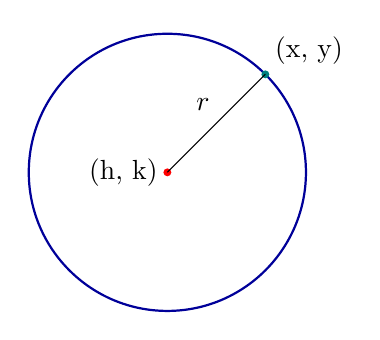
\begin{tikzpicture}[scale=1.1]
  \draw[blue!60!black, thick] (0,0) circle (1.6);
  \fill[red] (0,0) circle (1.3pt);
  \fill[teal] (45:1.6) circle (1.3pt);
  \draw[black] (0,0) -- (45:1.6);
  \node[left] at (0,0) {(h, k)};
  \node[above right] at (45:1.6) {(x, y)};
  \node[above left] at (45:0.85) {$r$};
\end{tikzpicture}
\end{center}
\figcaption{4.6}{A circle}

The equation of a circle with centre (h, k) and radius r is given as:

$(x - h)^2 + (y - k)^2 = r^2$, where $(x, y)$ is any point on the circumference of the
circle.

How did we come by this formula? The following activity will demonstrate.

\begin{activity}{Activity 4.2: Standard Equation of a Circle}
\textbf{Step 1:} Make a copy of the graph below. (a, b) is the centre of the circle and
$(x, y)$ is any point on the circumference of the circle.
\begin{center}
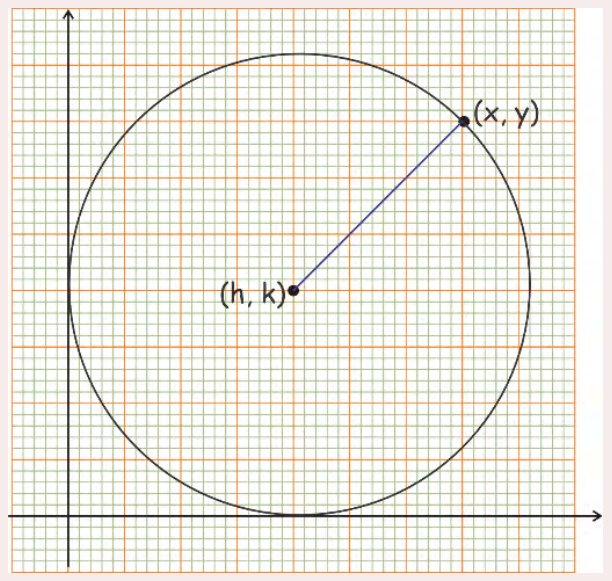
\includegraphics[width=0.45\linewidth]{figures/fig4-7.jpg}
\end{center}
\figcaption{4.7}{Graph of a circle}

\textbf{Step 2:} Using the radius as the hypotenuse, draw a right-angle triangle. Find
its horizontal and vertical distance.

\textbf{Step 3:} Using the Pythagoras theorem, write an equation to connect the
lengths of sides of the triangle.

Your answer should be similar to the one below:
\begin{center}
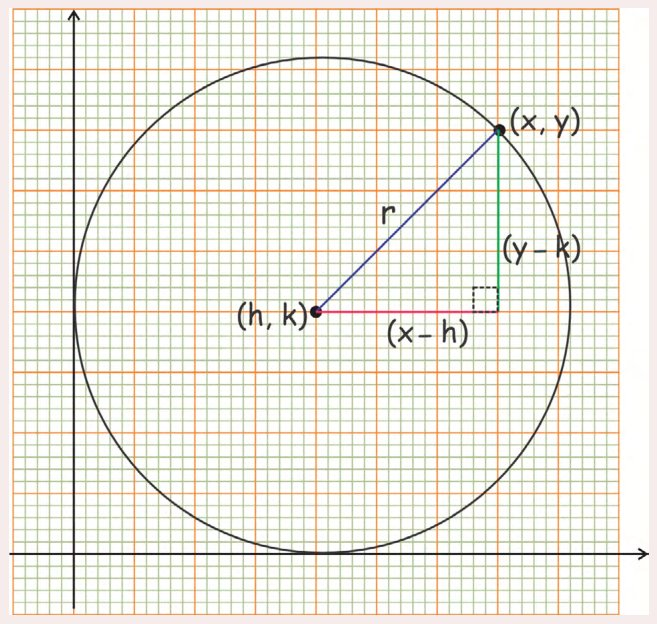
\includegraphics[width=0.48\linewidth]{figures/fig4-8.jpg}
\end{center}
\figcaption{4.8}{Graph of a circle}

From the figure, we have a right-angle triangle with hypotenuse, r, and the
lengths of the other sides as $(x - h)$ and $(y - k)$

Applying Pythagoras theorem, this gives:
\[ \boldsymbol{(x - h)^2 + (y - k)^2 = r^2} \]

Alternatively, you can find the distance between the centre (h, k) and any
point on the circumference (x, y) and you will achieve the same result
\[ r = \sqrt{(x - h)^2 + (y - k)^2} \]
Square both sides of the equation:
\[ \left(r\right)^2 = \left[\sqrt{(x - h)^2 + (y - k)^2}\right]^2 \qquad
   r^2 = (x - h)^2 + (y - k)^2 \]
Rearranging it, we have:
\[ \boldsymbol{(x - h)^2 + (y - k)^2 = r^2} \]
This gives the standard equation of a circle.
\end{activity}

Let us modify this equation for a few special scenarios.

\textbf{Scenario 1}: When the centre of the circle is the origin (0, 0).
\begin{center}
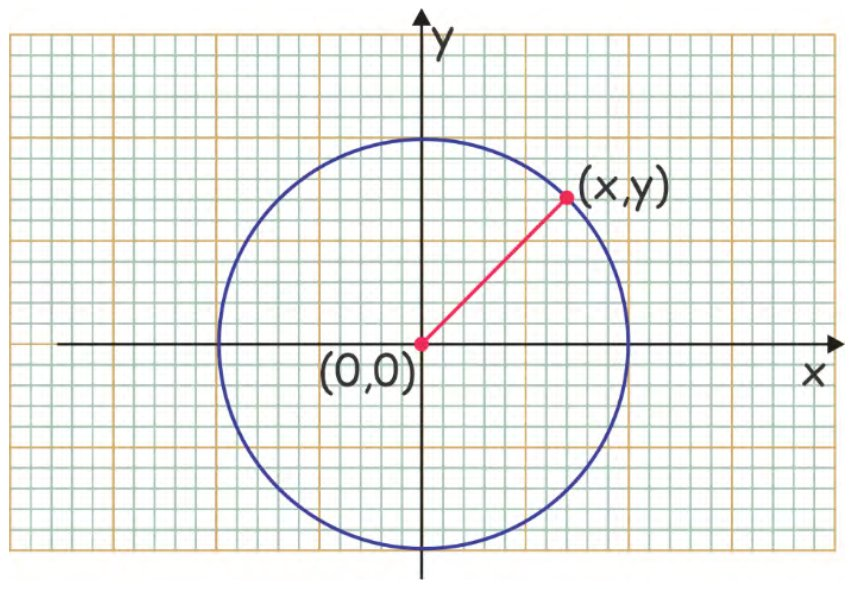
\includegraphics[width=0.6\linewidth]{figures/fig4-9.jpg}
\end{center}
\figcaption{4.9}{Graph of a circle}

When $(h, k) = (0, 0)$, the equation simplifies to:
\begin{align*}
(x - 0)^2 + (y - 0)^2 &= r^2 \\
x^2 + y^2 &= r^2
\end{align*}

\textbf{Scenario 2:} When the centre is any point on the x-axis other than (0, 0).
Remember that on the x-axis, y = 0.
\begin{center}
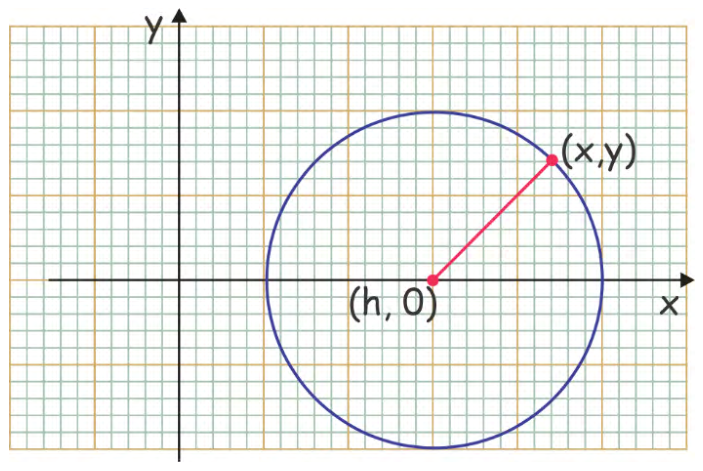
\includegraphics[width=0.5\linewidth]{figures/fig4-10.png}
\end{center}
\figcaption{4.10}{Graph of a circle}

So, we will use $(h, k) = (h, 0)$
\begin{align*}
(x - h)^2 + (y - 0)^2 &= r^2 \\
(x - h)^2 + y^2 &= r^2
\end{align*}

\textbf{Scenario 3:} When the centre is any point on the y-axis other than (o, 0).
Remember that on the y-axis, x=0.
\begin{center}
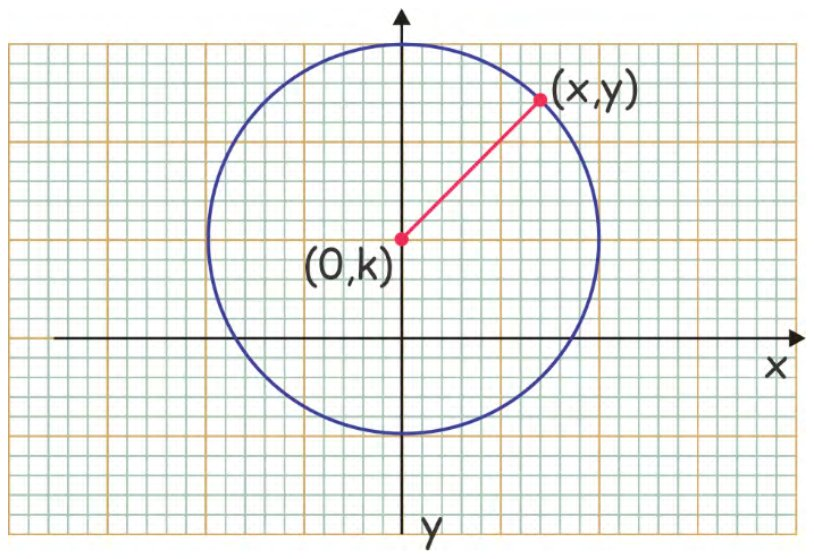
\includegraphics[width=0.55\linewidth]{figures/fig4-11.jpg}
\end{center}
\figcaption{4.11}{Graph of a circle}

So, we will use $(h, k) = (0, k)$
\begin{align*}
(x - 0)^2 + (y - k)^2 &= r^2 \\
x^2 + (y - k)^2 &= r^2
\end{align*}

\begin{example}{Example 4. 2}
Write the standard form of the circle equation with the following properties:
\begin{enumerate}
  \item[a.] Centre (1, 7) and radius 5
  \item[b.] Centre (3, 0) and radius $\frac{2}{3}$
  \item[c.] Centre (0, -5) and radius 2
  \item[d.] Centre (-6, -7) and radius 1
\end{enumerate}

\solution
The standard equation of a circle is given by $(x - h)^2 + (y - k)^2 = r^2$
\begin{enumerate}
  \item[a.] Centre (1, 7) and radius 5\\
  Using the standard equation, replace h with 1, k with 7 and r with 5\\
  $(x - 1)^2 + (y - 7)^2 = 5^2$\\
  $(x - 1)^2 + (y - 7)^2 = 25$
  \item[b.] Centre (3, 0) and radius $\frac{2}{3}$
  \item[c.] using the standard equation, replace h with 3, k with 0 and r with $\frac{2}{3}$
  \item[d.] $(x - 3)^2 + (y - 0)^2 = \left(\frac{2}{3}\right)^2$
  \item[e.] $(x - 3)^2 + y^2 = \frac{4}{9}$
  \item[f.] Centre (0, -5) and radius 2
  \item[g.] $(x - 0)^2 + (y - (-5))^2 = 2^2$
  \item[h.] $x^2 + (y + 5)^2 = 4$
  \item[i.] Centre (-6, -7) and radius 1\\
  $(x - (-6))^2 + (y - (-7))^2 = 1^2$\\
  $(x + 6)^2 + (y + 7)^2 = 1$
\end{enumerate}
\booknote[S4-03]{the solution is lettered a.\ to i.\ in the book: the working of
part (b) is lettered b--e, that of part (c) f--h and that of part (d) i.}
\end{example}

\begin{example}{Example 4.3}
\begin{enumerate}
  \item The diagram shows the graph of circles A, B and C. Use them to answer the
  following questions.
  \begin{center}
  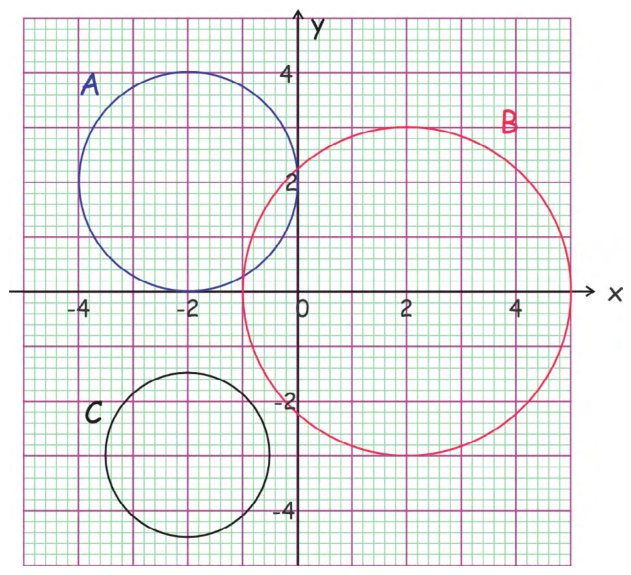
\includegraphics[width=0.5\linewidth]{figures/fig4-12.jpg}
  \end{center}
  \figcaption{4.12}{Graph of circles A, B and C}
  \begin{enumerate}
    \item[a.] Find the diameter of circle:
    \begin{enumerate}
      \item[i.] A
      \item[ii.] B
      \item[iii.] C
    \end{enumerate}
    \item[b.] Write in standard form the equation of:
    \begin{enumerate}
      \item[i.] A
      \item[ii.] B
      \item[iii.] C
    \end{enumerate}
  \end{enumerate}
  \item A phone's WI-FI has a range of 10m in all directions. If the phone is 2m
  West and 5m North, write an equation to represent the area within which the
  phone's Wi-Fi can operate.
\end{enumerate}

\solution
\begin{enumerate}
  \item \textbf{a.}
  \begin{enumerate}
    \item[i.] Diameter of A$=$ 4 units
    \item[ii.] Diameter of B$=$ 6 units
    \item[iii.] Diameter of C$=$ 3 units
  \end{enumerate}
  \textbf{b.}
  \begin{enumerate}
    \item[i.] The coordinates of the centre of circle A is $(-2, 2)$.\\
    Since the diameter is 4 units, it means the radius $= \frac{1}{2} \times 4 = 2$\\
    So, the equation of circle A is: $(x - (-2))^2 + (y - 2)^2 = 2^2$\\
    $(x + 2)^2 + (y - 2)^2 = 4$
    \item[ii.] The coordinates of the centre of circle B is (2, 0).\\
    Since the diameter is 6 units, it means the radius $= \frac{1}{2} \times 6 = 3$\\
    So, the equation of circle B is: $(x - 2)^2 + (y - 0)^2 = 3^2$\\
    $(x - 2)^2 + y^2 = 9$
    \item[iii.] The coordinates of the centre of circle C is $(-2, -3)$.\\
    Since the diameter is 3 units, it means the radius $= \frac{1}{2} \times 3 = \frac{3}{2}$\\
    So, the equation of circle C is: $(x - (-2))^2 + (y - (-3))^2 = \left(\frac{3}{2}\right)^2$\\
    $(x + 2)^2 + (y + 3)^2 = \frac{9}{4}$
  \end{enumerate}
  \item \mbox{}
  \begin{center}
  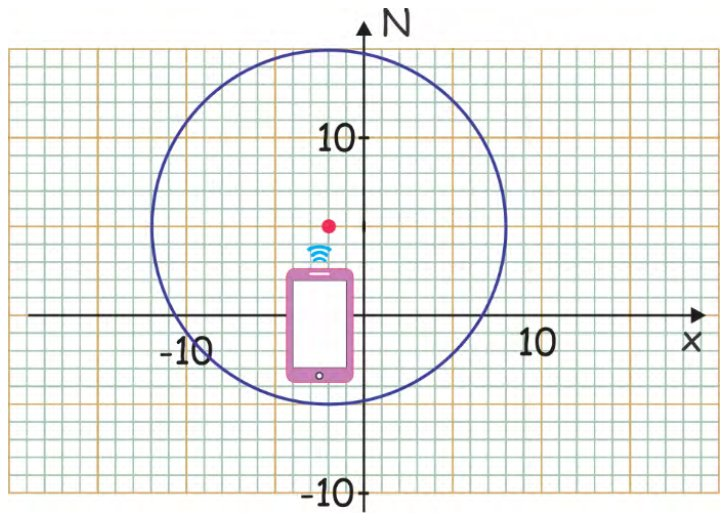
\includegraphics[width=0.55\linewidth]{figures/fig4-13.jpg}
  \end{center}
  \figcaption{4.13}{Graph of the range of the wi-fi signal}

  The range of the wi-fi signal is in the form of a circle with a radius of 10.

  2 units west and 5 units north are the same as the coordinates $(-2, 5)$. This
  point gives the centre of the wi-fi signal.

  The equation of the circle representing the range of the phone's wi-fi signals
  is:\\
  $(x - (-2))^2 + (y - 5)^2 = 10^2$\\
  $(x + 2)^2 + (y - 5)^2 = 100$
\end{enumerate}
\end{example}

\begin{example}{Example 4.4}
A Trotro driver operates within 40km at all angles from a lorry station. The lorry
station is located 15km south and 8km east of the driver's house.
\begin{enumerate}
  \item[a.] Write an equation to represent the driver's travel boundary from the lorry
  station using his house as the origin.
  \item[b.] Find the furthest distance between the driver's house and his travel boundary.
  \item[c.] Find the shortest distance between the driver's house and his travel boundary.
\end{enumerate}

\solution
\begin{center}
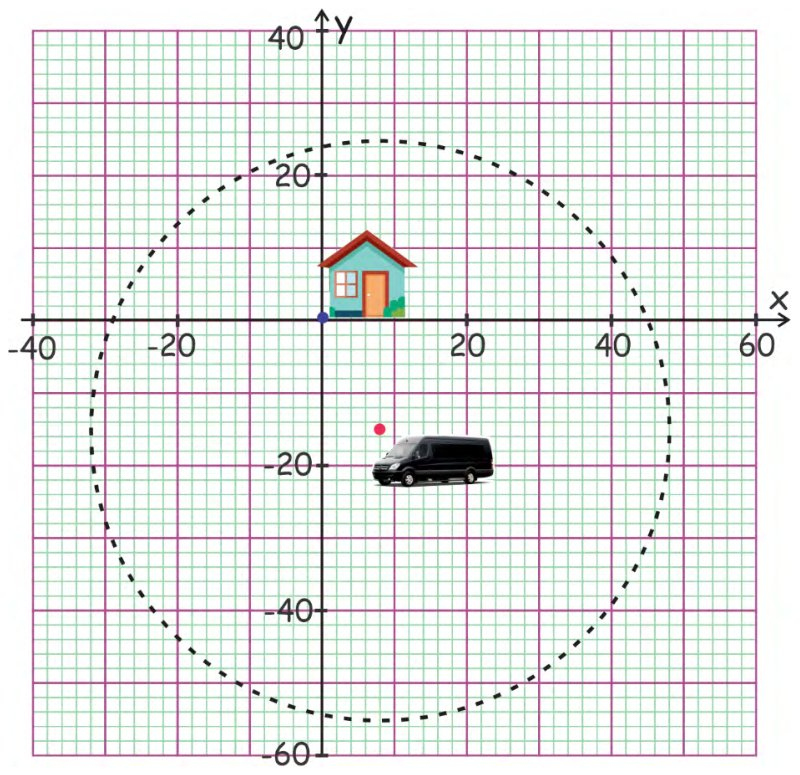
\includegraphics[width=0.6\linewidth]{figures/fig4-14.jpg}
\end{center}
\figcaption{4.14}{Graph of the lorry station and the driver's house}
\begin{enumerate}
  \item[a.] The driver's travel boundary is in the form of a circle with a radius of 40km.
  The centre is the lorry station. From his house, the lorry station is 15km
  south which represents $y = -15$ and 8km east which represents $x = 8$
  \item[b.] Thus, the centre $= (8, -15)$\\
  The equation of the driver's travel boundary is:\\
  $(x - 8)^2 + (y - (-15))^2 = 40^2$\\
  $(x - 8)^2 + (y + 15)^2 = 40^2$
  \item[c.] We first find the distance between the driver's house and the lorry station.
  \begin{align*}
  \text{Distance} &= \sqrt{8^2 + (-15)^2} \\
  &= \sqrt{64 + 225} \\
  &= \sqrt{289} = 17\text{km}
  \end{align*}
  Since his travel distance is 40km, it means the furthest the driver travels
  from his house is 17km $+$40km $=$ \textbf{57km}

  The shortest distance between the driver's house and his travel boundary is
  $40 - 17 = 23$ \textbf{km}
\end{enumerate}
\booknote[S4-04]{the labels b.\ and c.\ are misplaced in the book: ``Thus, the
centre $= (8, -15)$'' and the equation belong to part (a), while the answers to
(b) (57km) and (c) (23 km) both sit under c.}
\end{example}

\subsection{The general equation of a circle}

The general equation of a circle is: $x^2 + y^2 + 2gx + 2fy + c = 0$

To derive this formula, we will modify the standard equation.

We are going to replace the centre $(h, k)$ with $(-g, -f)$.

Recall that the standard equation of a circle is $(x - h)^2 + (y - k)^2 = r^2$ where $(h, k)$
is the centre and $r$ is the radius.

Replacing $(h, k)$ with $(-g, -f)$ we have:
\begin{align*}
(x - (-g))^2 + (y - (-f))^2 &= r^2 \\
(x + g)^2 + (y + f)^2 &= r^2
\end{align*}
Expanding the resulting equation, we get:
\begin{align*}
(x + g)(x + g) + (y + f)(y + f) &= r^2 \\
x^2 + gx + gx + g^2 + y^2 + fy + fy + f^2 &= r^2 \\
x^2 + 2gx + g^2 + y^2 + 2fy + f^2 &= r^2 \\
x^2 + y^2 + 2gx + 2fy + g^2 + f^2 - r^2 &= 0
\end{align*}
Since $g^2 + f^2 - r^2$ will simplify into a constant, replace it with C

This gives,
\[ \boldsymbol{x^2 + y^2 + 2gx + 2fy + c = 0} \]
Note that when the equation is written in the general form,
\begin{align*}
\text{the centre} = (-g, -f) &= \left(\frac{2g}{-2}, \frac{2f}{-2}\right) \\
&= \left(\frac{\textit{Coefficient of } x}{-2}, \frac{\textit{Coefficient of } y}{-2}\right) \\
&= -\frac{1}{2}(\textit{Coefficient of } x, \textit{Coefficient of } y)
\end{align*}
Also, $C = g^2 + f^2 - r^2$. Solving for $r$, we have
\begin{align*}
r^2 &= g^2 + f^2 - c \\
\sqrt{r^2} &= \sqrt{g^2 + f^2 - c} \\
\boldsymbol{r} &= \boldsymbol{\sqrt{g^2 + f^2 - c}}
\end{align*}

\begin{example}{Example 4.5}
Write the general equation of a circle with:
\begin{enumerate}
  \item[a.] Centre (1, 3) and radius 2.
  \item[b.] Centre $(-2, 4)$ and radius $\frac{1}{2}$
\end{enumerate}

\solution
Start from the standard equation and work through it to get the general equation.
\begin{enumerate}
  \item[a.] Centre (1, 3) and radius 2.
  \begin{align*}
  (x - 1)^2 + (y - 3)^2 &= 2^2 \\
  (x - 1)(x - 1) + (y - 3)(y - 3) &= 4 \\
  x^2 - 2x + 1 + y^2 - 6y + 9 &= 4 \\
  x^2 + y^2 - 2x - 6y + 9 + 1 - 4 &= 0 \\
  x^2 + y^2 - 2x - 6y + 6 &= 0
  \end{align*}
\end{enumerate}
Alternatively, we can solve for the variables in the general equation and then
substitute the answer into the general equation.
\begin{align*}
&x^2 + y^2 + 2gx + 2fy + c = 0 \\
&\text{The centre is } = (-g, -f) = (1, 3) \\
&\Longrightarrow g = -1 \text{ and } f = -3 \\
&C = (-1)^2 + (-3)^2 - 2^2 \\
&C = 1 + 9 - 4 \\
&\quad = 6
\end{align*}
Substituting these values into the general equation gives:
\begin{align*}
x^2 + y^2 + 2(-1)x + 2(-3)y + 6 &= 0 \\
x^2 + y^2 - 2x - 6y + 6 &= 0
\end{align*}
\begin{enumerate}
  \item[b.] Centre $(-2, 4)$ and radius $\frac{1}{2}$
  \begin{align*}
  (x - (-2))^2 + (y - 4)^2 &= \left(\frac{1}{2}\right)^2 \\
  (x + 2)(x + 2) + (y - 4)(y - 4) &= \frac{1}{4} \\
  x^2 + 4x + 4 + y^2 - 8y + 16 &= \frac{1}{4} \\
  x^2 + y^2 + 4x - 8y + 20 - \frac{1}{4} &= 0 \\
  x^2 + y^2 + 4x - 8y + \frac{79}{4} &= 0
  \end{align*}
  Multiply through by 4, so we only have integer values:
  \[ 4x^2 + 4y^2 + 16x - 32y + 79 = 0 \]
\end{enumerate}
Alternatively, we can solve for the variables in the general equation and then
substitute the answer into the general equation.
\begin{align*}
&x^2 + y^2 + 2gx + 2fy + c = 0 \\
&\text{The centre is } (-g, -f) = (-2, 4) \\
&\Longrightarrow g = 2 \text{ and } f = -4 \\
&C = (2)^2 + (-4)^2 - \left(\frac{1}{2}\right)^2 \\
&C = 4 + 16 - \frac{1}{4} \\
&C = 20 - \frac{1}{4} = \frac{79}{4}
\end{align*}
Substituting these values into the general equation gives:
\begin{align*}
x^2 + y^2 + 2(2)x + 2(-4)y + \frac{79}{4} &= 0 \\
x^2 + y^2 + 4x - 8y + \frac{79}{4} &= 0
\end{align*}
Multiply through by 4
\[ 4\boldsymbol{x}^2 + 4\boldsymbol{y}^2 + 16\boldsymbol{x} - 32\boldsymbol{y} + 79 = 0 \]
\end{example}

\begin{example}{Example 4.6}
Find the centre and radius of the following circle equations
\begin{enumerate}
  \item[a.] $x^2 + y^2 - 4x - 2y - 4 = 0$
  \item[b.] $x^2 + y^2 - 8x + 6y = 0$
  \item[c.] $x^2 + y^2 + 6x - 40 = 0$
  \item[d.] $4x^2 + 4y^2 - 8x + 3 = 0$
\end{enumerate}

\solution
\begin{enumerate}
  \item[a.] $x^2 + y^2 - 4x - 2y - 4 = 0$

  \textbf{Method 1:} Using completing the square method

  $x^2 - 4x + y^2 - 2y = 4$ group corresponding terms

  $(x^2 - 2x - 2x + 4) + (y^2 - y - y + 1) = 4 + 4 + 1$

  Expand and complete the square
  \begin{align*}
  (x - 2)^2 + (y - 1)^2 &= 9 \\
  (x - 2)^2 + (y - 1)^2 &= 3^2
  \end{align*}
  This shows that the centre is (2, 1) and the radius is 3

  \textbf{Method 2:} Alternatively, compare the given equation to the general equation
  of the circle and solve for the centre and the radius.

  The general equation of a circle is $x^2 + y^2 + 2gx + 2fy + c = 0$

  The given equation is $x^2 + y^2 - 4x - 2y - 4 = 0$

  $x^2 + y^2 + 2(-2)x + 2(-1)y + (-4) = 0$

  By comparing coefficients, we have $g = -2 \Longrightarrow -g = 2$

  Also, $f = -1 \Longrightarrow -f = 1$ and $c = -4$

  Recall that when the circle equation is written in the general form, the centre
  is $(-g, -f)$

  Therefore, the centre is (2, 1).

  You will achieve the same result if you divide the coefficient of $x$ and $y$ by $-2$

  Centre $= (-4 \_\, -2, -2 \_\, -2) = (2, 1)$
  \booknote[S4-05]{the division signs are printed as underscores; read
  $(-4 \div -2,\ -2 \div -2)$.}

  Radius $= r = \sqrt{g^2 + f^2 - c}$

  $r = \sqrt{2^2 + 1^2 - (-4)} = \sqrt{9} = 3$

  \item[b.] $x^2 + y^2 - 8x + 6y = 0$

  \textit{Method 1}: Using the completing the square method, we have:
  \begin{align*}
  x^2 - 8x + 16 + y^2 + 6y + 9 &= 16 + 9 \\
  (x - 4)^2 + (y + 3)^2 &= 25 \\
  (x - 4)^2 + (y + 3)^2 &= 5^2
  \end{align*}
  Therefore, the centre is (4, -3) and the radius is 5

  \textbf{Method 2:} Alternatively, we can re-write the equation as

  $x^2 + y^2 + 2(-4)x + 2(3)y + 0 = 0$

  Comparing this equation to $x^2 + y^2 + 2gx + 2fy + c = 0$, we have:

  $g = -4 \Longrightarrow -g = 4$, $f = 3 \Longrightarrow -f = -3$ and C$=0$

  Therefore, the centre is (4, -3)

  Radius $= r = \sqrt{(-4)^2 + 3^2 - 0} = \sqrt{25} = 5$

  \item[c.] $x^2 + y^2 + 6x - 40 = 0$

  \textbf{Method 1:} Completing the square, we have:
  \begin{align*}
  x^2 + 6x + 9 + y^2 + 2(0)x + 0 &= 40 + 9 + 0 \\
  (x + 3)^2 + (y + 0)^2 &= 49 \\
  (x + 3)^2 + (y + 0)^2 &= 7^2
  \end{align*}
  Centre is (-3, 0) and radius is 7

  \textbf{Method 2:} Alternatively, we can re-write the equation as

  $x^2 + y^2 + 2(3)x + 2(0)y - 40 = 0$

  Comparing this equation to $x^2 + y^2 + 2gx + 2fy + c = 0$, we have:

  $g = 3 \Longrightarrow -g = -3$, $f = 0 \Longrightarrow -f = 0$ and C$= -40$

  Therefore, the centre is (-3, 0)

  Radius $= r = \sqrt{(3)^2 + 0^2 - (-40)} = \sqrt{49} = 7$

  \item[d.] $4x^2 + 4y^2 - 8x + 3 = 0$

  Method 1: Completing the square, we will first divide the equation by 4

  $x^2 + y^2 - 2x + \frac{3}{4} = 0 \quad x^2 - 2x + 1 + y^2 + 0 = -\frac{3}{4} + 1 + 0$

  $(x - 1)^2 + (y + 0)^2 = 1 \_\, 4$

  $\left(x - 1\right)^2 + \left(y + 0\right)^2 = \left(\frac{1}{2}\right)^2$
  \booknote[S4-06]{two equations are run together on one line, and the right-hand
  side of the next line is printed ``$1 \_\, 4$'' for $\frac{1}{4}$.}

  Centre is (1, 0) and radius is $\frac{1}{2}$

  \textbf{Method 2:} Alternatively, we can re-write the equation as:

  $x^2 + y^2 + 2(-1)x + 2(0)y + \frac{3}{4} = 0$

  Comparing this equation to $x^2 + y^2 + 2gx + 2fy + c = 0$, we have:

  $g = -1 \Longrightarrow -g = 1$, $f = 0 \Longrightarrow -f = 0$ and C$= \frac{3}{4}$

  Therefore, the centre is (1, 0)

  Radius $= r = \sqrt{(-1)^2 + 0^2 - \frac{3}{4}} = \sqrt{\frac{1}{4}} = \frac{1}{2}$
\end{enumerate}
\end{example}

% Book pp. 151-158 (PDF pp. 152-159)
\section{Deriving the Equations of a Circle from Given Points}

\subsection{How to Find the Equation of the Circle Given the Endpoints of the Diameter}

\textit{Method 1:}

\textbf{Step 1:} Find the centre of the circle by finding the mid-point of the diameter.

\textbf{Step 2:} Calculate the length of the radius. This is half the diameter and is the
same as the distance between the centre and any of the endpoints of the diameter.

\textbf{Step 3:} Substitute the centre and the radius into the standard equation of the
circle.

\textbf{Step 4:} Simplify the resulting equation to achieve the desired result.

\textit{Method 2:}

An alternative method involves using the relationship between gradients of two
perpendicular lines.

Recall that if $m_1$ and $m_2$ are gradients of any two lines which intersect at right
angles, then $m_1 \times m_2 = -1$

Also, if one side of a triangle inscribed in a circle is a diameter, then the triangle
is right-angled. The angle opposite the diameter is the right angle. This property
of circles is illustrated in the diagram below.
\begin{center}
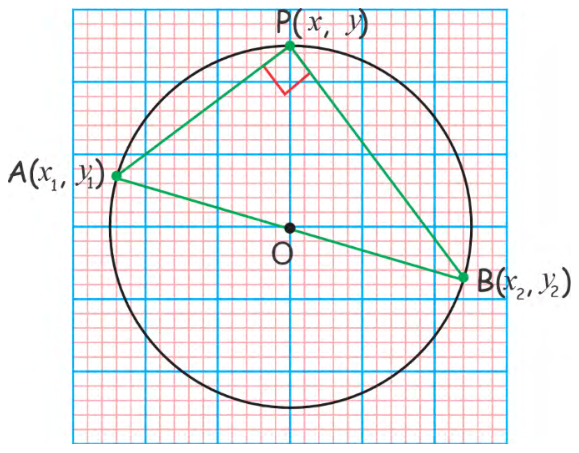
\includegraphics[width=0.42\linewidth]{figures/fig4-15.png}
\end{center}
\figcaption{4.15}{Graph of circle with centre O}

From the figure, $A(x_1, y_1)$ and $B(x_2, y_2)$ are the endpoints of the diameter and $P(x, y)$
is any point on the circumference of the circle. The angle opposite the diameter
is AOB$= 90^\circ$. This means that the product to the gradients of lines AP and BP is
equal to $-1$. Using this relation will generate the equation of the circle.
\booknote[S4-08]{the right angle is at P, so this should read APB $= 90^\circ$; O is
the centre.}
\begin{align*}
\text{Gradient } (m_1) \text{ of } |\text{AP}| &= \frac{y - y_1}{x - x_1} \\
\text{Gradient } (m_2) \text{ of } |\text{BP}| &= \frac{y - y_2}{x - x_2}
\end{align*}
Using $m_1 \times m_2 = -1$, we have
\[ \frac{y - y_1}{x - x_1} \times \frac{y - y_2}{x - x_2} = -1 \]

\begin{example}{Example 4.7}
The endpoints of the diameter of a circle are (-2, 2) and (4, -6).

Find the;
\begin{enumerate}
  \item[a.] radius and centre of the circle
  \item[b.] general equation of the circle.
\end{enumerate}

\solution
The graph below shows a sketch of the circle.
\begin{center}
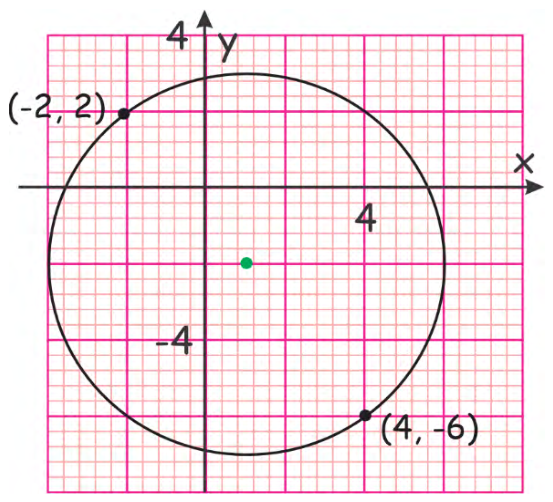
\includegraphics[width=0.42\linewidth]{figures/fig4-16.png}
\end{center}
\figcaption{4.16}{Graph of circle with diameter (-2, 2) and (4, -6)}

\textit{Method 1:}
\begin{enumerate}
  \item The centre is equal to the mid-point of the endpoints of the diameter
  \item Midpoint $= \frac{1}{2}(-2 + 4, 2 + (-6))$
  \item $= \frac{1}{2}(2, -4)$
  \item $= \left(\frac{2}{2}, -\frac{4}{2}\right) = \left(1, -2\right)$
\end{enumerate}
\booknote[S4-07]{the four lines of this working are numbered 1.\ to 4.\ in the
book, as if they were separate parts.}

Radius is the distance between the centre and any of the endpoint/point on the
circumference.
\begin{align*}
r &= \sqrt{(-6 - (-2))^2 + (4 - 1)^2} \\
r &= \sqrt{(-4)^2 + 3^2} \\
r &= \sqrt{16 + 9} \\
&= \sqrt{25} = 5
\end{align*}
Using $(x - h)^2 + (y - k)^2 = r^2$, we have:
\begin{align*}
(x - 1)^2 + (y - (-2))^2 &= 5^2 \\
(x - 1)^2 + (y + 2)^2 &= 25 \\
x^2 - 2x + 1 + y^2 + 4y + 4 &= 25 \\
x^2 + y^2 - 2x + 4y + 5 &= 25 \\
x^2 + y^2 - 2x + 4y + 5 - 25 &= 0 \\
\boldsymbol{x^2 + y^2 - 2x + 4y - 20} &= \boldsymbol{0}
\end{align*}

\textit{Method 2:}

Alternatively, let any point on the circumference of the circle be P(x, y) as shown
in the figure below.
\begin{center}
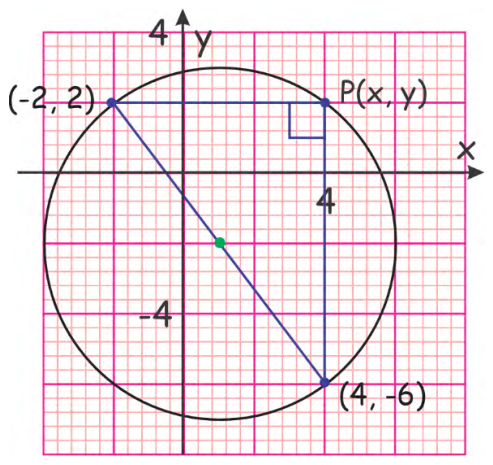
\includegraphics[width=0.4\linewidth]{figures/fig4-17.png}
\end{center}
\figcaption{4.17}{Graph of circle with diameter (-2, 2) and (4, -6)}

The gradient of the line connecting (-2, 2) and $(x, y) = \dfrac{-2}{x - (-2)} = \dfrac{y - 2}{x + 2}$
\booknote[S4-09]{the first numerator is printed as $-2$; it should be $y - 2$, as
the second fraction shows.}

The gradient of the line connecting (4, -6) and $(x, y) = \dfrac{y - (-6)}{x - 4} = \dfrac{y + 6}{x - 4}$

Since the two lines intersect at $90^\circ$,
\begin{align*}
\left(\frac{y - 2}{x + 2}\right) \times \left(\frac{y + 6}{x - 4}\right) &= -1 \\
\frac{(y - 2)(y + 6)}{(x + 2)(x - 4)} &= -1 \\
\frac{y^2 + 6y - 2y - 12}{x^2 - 4x + 2x - 8} &= -1 \\
\frac{y^2 + 4y - 12}{x^2 - 2x - 8} &= -\frac{1}{1}
\end{align*}
Cross multiply:
\begin{align*}
y^2 + 4y - 12 &= -1(x^2 - 2x - 8) \\
y^2 + 4y - 12 &= -x^2 + 2x + 8
\end{align*}
Regroup the terms:
\begin{align*}
y^2 + x^2 - 2x + 4y - 12 - 8 &= 0 \\
\boldsymbol{y^2 + x^2 - 2x + 4y - 20} &= \boldsymbol{0}
\end{align*}
\end{example}

\subsection{Equation of a Circle Given Three Points on the Circumference of the Circle}

\textit{Method 1:}

Substitute each of the points into the general equation of the circle
$(x^2 + y^2 + 2gx + 2fy + c = 0)$.

This results in 3 simultaneous equations with 3 unknowns to be solved for $g$, $f$
and $c$.

\textit{Method 2}:

Alternatively, follow the following steps.

\textbf{Step 1:} Find the equation of the perpendicular bisectors of any two of the chords.

In the Figure 4.18 A, B and C are points on the circumference of the circle.
\begin{center}
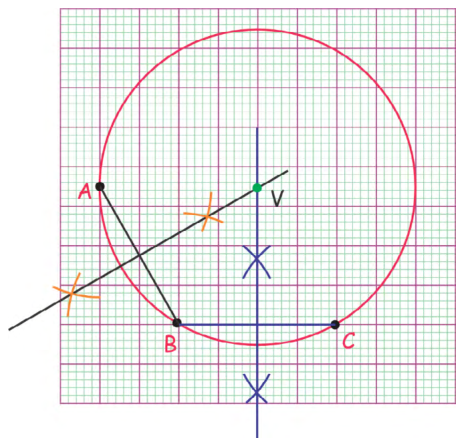
\includegraphics[width=0.38\linewidth]{figures/fig4-18.png}
\end{center}
\figcaption{4.18}{Graph of circle with equation $(x^2 + y^2 + 2gx + 2fy + c = 0)$}

\textbf{Step 2:} Solve the equations obtained in step 1 simultaneously. This will give the
coordinates of the centre of the circle.

\textbf{Step 3:} Using the centre and any point on the circumference, calculate the radius.

\textbf{Step 4:} Use the radius and the centre to calculate the equation of the circle.

\begin{example}{Example 4.8}
Find the equation of the circle which satisfies the points (2, -4), (-6, 4) and (2, 12).

\solution
\textit{Method 1}:

In the diagram below, A, B and C are points on the circumference of the circle.
The perpendicular bisectors of chords AB and BC intersect at point V. Point V is
the centre of the circle.
\begin{center}
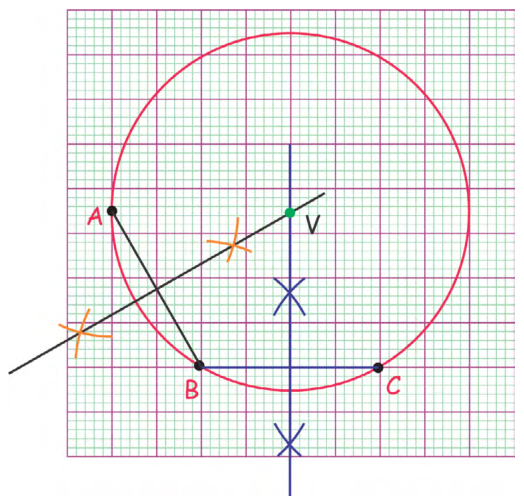
\includegraphics[width=0.42\linewidth]{figures/fig4-19.png}
\end{center}
\figcaption{4.19}{Graph of circle with points (2, -4), (-6, 4) and (2, 12)}

Substitute the points into the general equation of the circle.

Substituting (-6, 4) into $x^2 + y^2 + 2gx + 2fy + c = 0$ gives:
\begin{align*}
(-6)^2 + 4^2 + 2g(-6) + 2f(4) + c &= 0 \\
36 + 16 - 12g + 8f + c &= 0 \\
-12g + 8f + c &= -52 \ldots\ldots\ldots\ldots\ldots\ldots\ldots\ldots..(1)
\end{align*}
Substituting (2, 12) into the same equation:
\begin{align*}
(2)^2 + (12)^2 + 2g(2) + 2f(12) + c &= 0 \\
4 + 144 + 4g + 24f + c &= 0 \\
4g + 24f + c &= -148 \ldots\ldots\ldots\ldots\ldots\ldots\ldots\ldots\ldots...(2)
\end{align*}
Substituting (2, -4) into the same equation:
\begin{align*}
(2)^2 + (-4)^2 + 2g(2) + 2f(-4) + c &= 0 \\
4 + 16 + 4g - 8f + c &= 0 \\
4g - 8f + c &= -20 \ldots\ldots\ldots\ldots\ldots\ldots\ldots\ldots\ldots\ldots\ldots. (3)
\end{align*}
Subtract (2) from (3). That is (3) -- (2)
\begin{align*}
(4g - 8f + c) - (4g + 24f + c) &= -20 - (-148) \\
4g - 8f + c - 4g - 24f - c &= -20 + 148 \\
-32f &= 128 \\
f &= -\frac{128}{32} = -4
\end{align*}
Subtract (1) from (2):
\begin{align*}
(4g + 24f + c) - (-12g + 8f + c) &= -148 - (-52) \\
4g + 24f + c + 12g - 8f - c &= -148 + 52 \\
16g + 16f &= -96 \\
16g + 16(-4) &= -96 \\
16g - 64 &= -96 \\
16g &= -96 + 64 \\
\frac{16g}{16} &= -\frac{32}{16} \\
g &= -2
\end{align*}
Substitute $g = -2$ and $f = -4$ into (3):
\begin{align*}
4(-2) - 8(-4) + c &= -20 \\
-8 + 32 + c &= -20 \\
c &= -20 + 8 - 32 \\
c &= -44
\end{align*}
Finally, substitute $g$, f and c into the general equation.

$x^2 + y^2 + 2(-2)x + 2(-4)y - 44 = 0$

$\boldsymbol{x^2 + y^2 - 4x - 8y - 44 = 0}$ gives the equation of the circle which satisfies
$(2, -4)$, $(-6, 4)$ and $(2, 12)$.

\textit{Method 2}:

First plot the points on the x-y plane and connect the points with chords.
\begin{center}
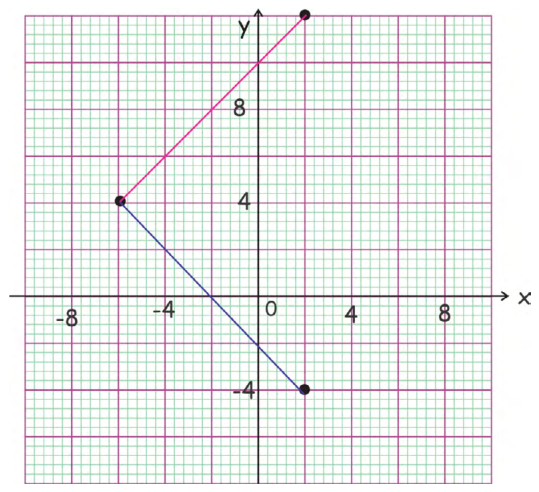
\includegraphics[width=0.42\linewidth]{figures/fig4-20.png}
\end{center}
\figcaption{4.20}{Graph of the $x$-$y$ plane}

Mid-point of $(-6, 4)$ and $(2, 12)$ is $\left(\dfrac{-6 + 2}{2}, \dfrac{4 + 12}{2}\right) = \left(-2, 8\right)$

The gradient of the line connecting the points $(-6, 4)$ and $(2, 12)$ is
\[ \frac{12 - 4}{2 - (-6)} = \frac{8}{8} = 1 \]
The gradient of the perpendicular bisector is $-1$

The equation of the perpendicular bisector is $y - 8 = -1(x - (-2))$
\begin{align*}
y &= -1(x + 2) + 8 \\
y &= -x - 2 + 8 \\
y &= -x + 6 \ldots\ldots\ldots\ldots\ldots\ldots\ldots\ldots.(1)
\end{align*}
Mid-point of $(-6, 4)$ and $(2, -4)$ is $\left(\dfrac{-6 + 2}{2}, \dfrac{4 - 4}{2}\right) = \left(-2, 0\right)$

The gradient of the line connecting the points $(-6, 4)$ and $(2, -4)$ is
\[ \frac{-4 - 4}{2 - (-6)} = \frac{-8}{8} = -1 \]
The gradient of the perpendicular bisector is 1

The equation of the perpendicular bisector is $y - 0 = 1(x - (-2))$
\begin{align*}
y &= (x + 2) \\
y &= x + 2 \\
y &= x + 2 \ldots\ldots\ldots\ldots\ldots\ldots\ldots\ldots.(2)
\end{align*}
Add equation 1 to equation 2:
\begin{align*}
y + y &= -x + x + 6 + 2 \\
2y &= 8 \\
y &= 4
\end{align*}
Substitute $y = 4$ into equation 2 and solve for $x$:
\begin{align*}
4 &= x + 2 \\
x &= 4 - 2 \\
x &= 2
\end{align*}
This means the coordinates of the centre of the circle is (2, 4).

The distance between the centre and any point on the circle's circumference gives
the radius.
\begin{align*}
\text{Distance between (2, 4) and (2, 12)} = r &= \sqrt{(2 - 2)^2 + (12 - 4)^2} \\
&= \sqrt{0^2 + 8^2} \\
&= \sqrt{64} \\
&= 8
\end{align*}
Finally, substitute the centre, (2, 4), and the radius, 8, into the standard equation
of the circle.
\begin{align*}
(x - 2)^2 + (y - 4)^2 &= 8^2 \\
x^2 - 4x + 4 + y^2 - 8y + 16 &= 64 \\
x^2 + y^2 - 4x - 8y + 20 - 64 &= 0 \\
\boldsymbol{x^2 + y^2 - 4x - 8y - 44} &= \boldsymbol{0}
\end{align*}
A construction of the circle is shown below
\begin{center}
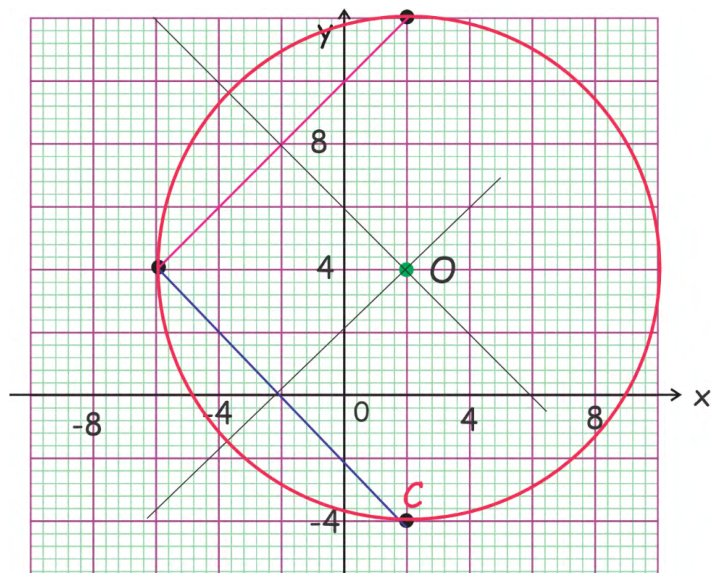
\includegraphics[width=0.55\linewidth]{figures/fig4-21.jpg}
\end{center}
\figcaption{4.21}{Graph of circle $x^2 + y^2 - 4x - 8y - 44 = 0$}
\end{example}

% Book pp. 159-165 (PDF pp. 160-166)
\section{Tangents and Normals}

\begin{center}
\textbf{\color{sectionblue} Study Figure 4.22 carefully:}
\end{center}
\begin{center}
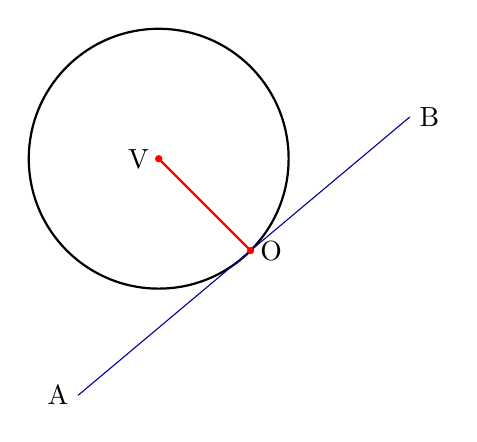
\begin{tikzpicture}[scale=1.1]
  \coordinate (V) at (0,0);
  \coordinate (O) at (-45:1.5);
  \draw[black, thick] (V) circle (1.5);
  \draw[blue!60!black] ($(O)+(-140:2.6)$) -- ($(O)+(40:2.4)$);
  \draw[red, thick] (V) -- (O);
  \fill[red] (V) circle (1.2pt);
  \fill[red] (O) circle (1.2pt);
  \node[left] at (V) {V};
  \node[right] at (O) {O};
  \node[left] at ($(O)+(-140:2.6)$) {A};
  \node[right] at ($(O)+(40:2.4)$) {B};
\end{tikzpicture}
\end{center}
\figcaption{4.22}{Tangent of a circle}

In Figure 4.22, V is the circle's centre, $|$VO$|$ is a radius and AOB is a tangent to the
circle at O. The tangent is a line that touches the circle at only one point.

The equation of the radius, VO, or its extension is the normal to tangent, AOB.
The normal and the tangent intersect at right angles at the point of tangency.

Since $|$VO$|$ and $|$AOB$|$ intersect at right angles,

We have the (gradient of $|$OV$|$ )$\times$ (gradient of $|AOB|$) $= -1$

Let us use this relation to answer a few questions.

\subsection{How to find the equation of a tangent and normal given the circle
equation and a point, $(a, b)$, on the circumference of the circle}

\textbf{Step 1:} Using the given circle equation, find the centre, (h, k)

\textbf{Step 2:} Find the gradient of the normal. This is the gradient (m) of the line
connecting points (h, k) and (a, b)

\textbf{Step 3:} Find the gradient of the tangent. The gradient of the tangent is $-\frac{1}{m}$, where
$m$ is the gradient of the normal.

\textbf{Step 4:} Find the equation of the tangent. This is given as:
\[ y - b = -\frac{1}{m}(x - a) \]
The equation of the normal is $y - k = m(x - h)$

Where $(a, b)$ is a point on the circumference of the circle and (h, k) is the centre
of the circle.

\begin{example}{Example 4.9}
Find the equations of the line tangent and normal to the circle $x^2 + y^2 = 169$ at
point $(5, -12)$

\solution
First find the centre of the circle.

To do this, we will write the equation in the standard form:
\[ (x - 0)^2 + (y - 0)^2 = 13^2 \]
This is a circle with a centre (0, 0) and a radius of 13 units.

Next, we will check if the given point satisfies the circle equation.
\[ 5^2 + (-12)^2 = 25 + 144 = 169 \]
This shows that $(5, -12)$ is on the circumference of the circle.

Next, find the gradient of the normal. This is the gradient of the line connecting
the points (0, 0) and (5, -12)
\[ m = -\frac{12 - 0}{5 - 0} = -1\tfrac{2}{5} \]
\booknote[S4-10]{$-\frac{12}{5}$ is printed as the mixed number $-1\frac{2}{5}$; it is
$-2\frac{2}{5}$. Below, the gradient of the tangent is printed as
``$-\frac{1}{m} = -\frac{\frac{1}{12}}{5} = 1 \times \frac{5}{12} = \frac{5}{12}$''; it should
read $-\frac{1}{m} = -\dfrac{1}{-\frac{12}{5}} = 1 \times \frac{5}{12} = \frac{5}{12}$.}
Equation of the normal is: $y - 0 = -\frac{12}{5}(x - 0)$

Multiply through by 5:
\[ 5y = -12x \]
$5y + 12x = 0$ is the equation of the normal.

The gradient of the tangent is $= -\dfrac{1}{m} = -\dfrac{\frac{1}{12}}{5} = 1 \times \dfrac{5}{12} = \dfrac{5}{12}$

The equation of the tangent is: $y - (-12) = \frac{5}{12}(x - 5)$
\[ (y + 12) = \frac{5}{12}(x - 5) \]
Multiply through by 12:
\begin{align*}
12y + 144 &= 5x - 25 \\
12y - 5x + 144 + 25 &= 0
\end{align*}
$12\boldsymbol{y} - 5\boldsymbol{x} + 169 = 0$ is the equation of the tangent.
\end{example}

\begin{example}{Example 4.10}
The point (5, 3) satisfies the equation $x^2 + y^2 - 6x - 4y + 8 = 0$.
\begin{enumerate}
  \item[a.] Find the radius of the circle.
  \item[b.] Fine the equation of the normal to the circle at point (5, 3)
  \item[c.] Find the equation of the tangent to the circle at (5, 3)
\end{enumerate}

\solution
\begin{enumerate}
  \item[a.] To find the radius, write the equation in standard form
  \begin{align*}
  x^2 - 6x + 9 + y^2 - 4y + 4 &= -8 + 9 + 4 \\
  (x - 3)^2 + (y - 2)^2 &= 5 \\
  \left(x - 3\right)^2 + \left(y - 2\right)^2 &= \left(\sqrt{5}\right)^2
  \end{align*}
  This means the \textbf{radius is} $\sqrt{5}$ \textbf{and the centre is} (3, 2).

  Gradient of the normal.

  This is the gradient of the line connecting the points (3, 2) and (5, 3)
  \item[b.] The gradient of the normal $= \dfrac{3 - 2}{5 - 3} = \dfrac{1}{2}$

  The equation of the normal is: $y - 2 = \frac{1}{2}(x - 3)$
  \begin{align*}
  2y - 4 &= x - 3 \\
  2y - x - 4 + 3 &= 0 \\
  2\boldsymbol{y} - \boldsymbol{x} - 1 &= 0
  \end{align*}
  Gradient of the tangent $= -1 \div \frac{1}{2} = -2$
  \item[c.] The equation of the tangent is:
  \begin{align*}
  y - 3 &= -2(x - 5) \\
  y - 3 &= -2x + 10 \\
  \boldsymbol{y} + 2\boldsymbol{x} - 13 &= 0
  \end{align*}
\end{enumerate}
\end{example}

\begin{example}{Example 4.11}
Find the equation of the normal to the circle $y^2 + x^2 + 8x + 7 = 0$ that passes
through the point (1, 3)

\solution
First, verify if the point lies on the circumference of the circle:
\[ (3)^2 + (1)^2 + 8(1) + 7 \ne 0 \]
Therefore, the point (1, 3) is not on the circle's circumference.

Next, find the coordinates of the centre of the circle.
\begin{align*}
\text{The centre is given as} = {} & \left(\frac{\textit{coefficient of } x}{-2}, \frac{\textit{coefficient of } y}{-2}\right) \\
= {} & \left(\frac{8}{-2}, \frac{0}{-2}\right) \\
= {} & (-4, 0)
\end{align*}
The gradient of the normal $= \dfrac{-3}{-4 - 1} = \dfrac{3}{5}$

Equation of the normal: $y - 3 = \frac{3}{5}(x - 1)$
\begin{align*}
5y - 15 &= 3x - 3 \\
5y - 3x - 15 + 3 &= 0 \\
5\boldsymbol{y} - 3\boldsymbol{x} - 12 &= 0
\end{align*}
The diagram below shows the construction of the circle and the normal
\begin{center}
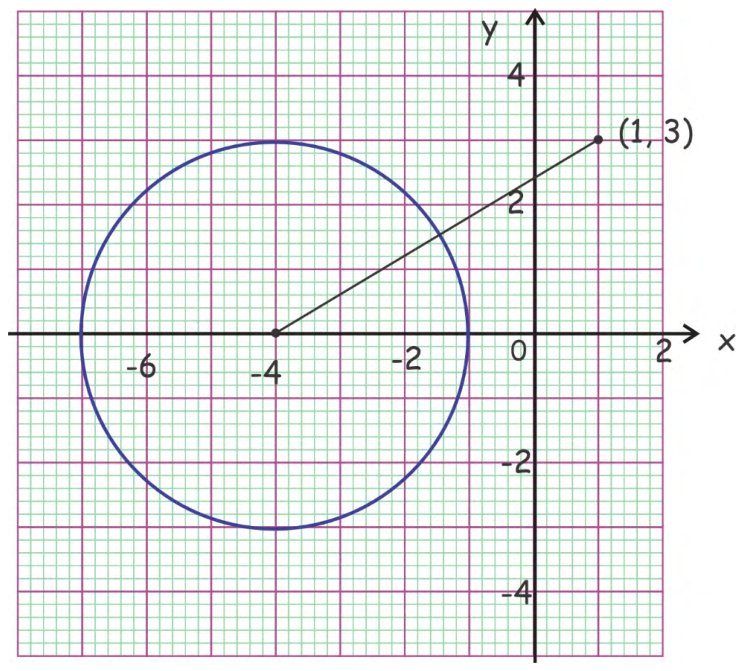
\includegraphics[width=0.6\linewidth]{figures/fig4-23.jpg}
\end{center}
\figcaption{4.23}{Construction of a circle and normal}
\end{example}

\subsection{Length of a tangent (L)}

Given the equation of a circle, it is possible to find the length of a tangent to the
circle from a point $(x, y)$ outside the circle.

Figure 4.24 illustrates this:
\begin{center}
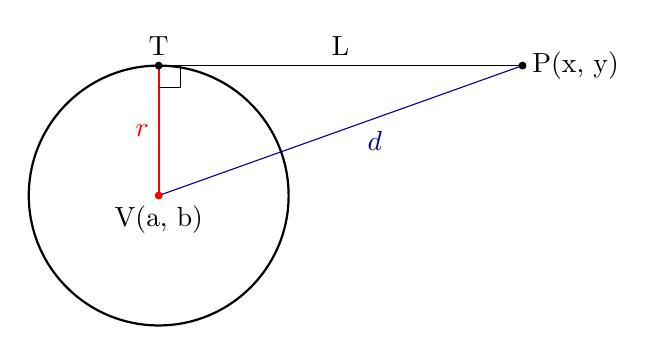
\begin{tikzpicture}[scale=1.1]
  \coordinate (V) at (0,0);
  \coordinate (T) at (0,1.5);
  \coordinate (P) at (4.2,1.5);
  \draw[black, thick] (V) circle (1.5);
  \draw[black] (T) -- (P);
  \draw[blue!60!black] (V) -- (P);
  \draw[red, thick] (V) -- (T);
  \draw (0,1.5) ++(0.25,0) -- ++(0,-0.25) -- ++(-0.25,0);
  \fill[red] (V) circle (1.3pt);
  \fill[black] (T) circle (1.3pt);
  \fill[black] (P) circle (1.3pt);
  \node[above] at (T) {T};
  \node[above] at (2.1,1.5) {L};
  \node[right] at (P) {P(x, y)};
  \node[below] at (V) {V(a, b)};
  \node[red, left] at (0,0.75) {$r$};
  \node[blue!60!black, below right] at (2.3,0.85) {$d$};
\end{tikzpicture}
\end{center}
\figcaption{4.24}{Length of a tangent}

In Figure 4.24, V(a, b) is the centre of the circle. T is a point of tangency and P($x$,
$y$) is any point outside the circle. The length of the tangent is $|$PT$| = L$.

From Pythagoras' theorem, we have $L^2 + r^2 = d^2$, since we are interested in
finding L, make it the subject.
\begin{align*}
L^2 &= d^2 - r^2 \\
\sqrt{L^2} &= \sqrt{d^2 - r^2} \\
L &= \sqrt{d^2 - r^2}
\end{align*}

\begin{example}{Example 4.12}
Find the length of the tangent from the point (0, 4) to the circle $x^2 + y^2 - 2x +
12y - 3 = 0$
\booknote[S4-11]{the circle worked in the solution (and named in the caption of
Figure 4.25) is $x^2 + y^2 - 6x + 4y - 3 = 0$, with centre $(3, -2)$ and radius 4;
the equation printed in the question does not match it. For the circle as
printed, the centre is $(1, -6)$, $r^2 = 40$, $d^2 = 101$ and the length is
$\sqrt{61}$.}

\solution
First find the centre and radius of the circle:
\begin{align*}
x^2 - 6x + 9 + y^2 + 4y + 4 - 3 &= 9 + 4 \\
(x - 3)^2 + (y + 2)^2 &= 16 \\
(x - 3)^2 + (y + 2)^2 &= 4^2
\end{align*}
The centre of the circle is (3, -2) and the radius is 4
\begin{center}
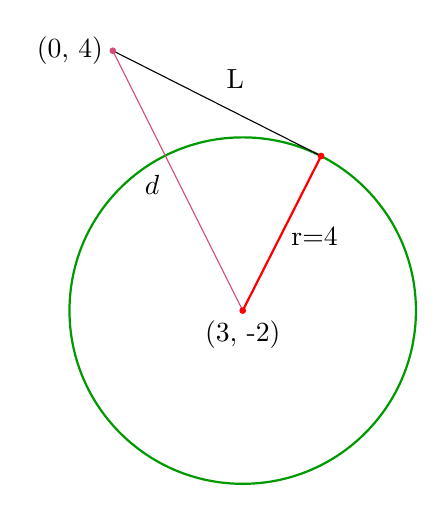
\begin{tikzpicture}[scale=0.55]
  \coordinate (C) at (3,-2);
  \coordinate (P) at (0,4);
  \coordinate (T) at (4.81,1.57);
  \draw[green!60!black, thick] (C) circle (4);
  \draw[purple!70] (C) -- (P);
  \draw[black] (P) -- (T);
  \draw[red, thick] (C) -- (T);
  \fill[purple!70] (P) circle (2.2pt);
  \fill[red] (C) circle (2.2pt);
  \fill[red] (T) circle (2.2pt);
  \node[left] at (P) {(0, 4)};
  \node[below] at (C) {(3, -2)};
  \node[above right] at (2.4,2.9) {L};
  \node[left] at (1.3,0.9) {$d$};
  \node[right] at (3.9,-0.3) {r=4};
\end{tikzpicture}
\end{center}
\figcaption{4.25}{Length of the tangent to the circle $x^2 + y^2 - 2x + 12y - 3 = 0$}

Distance between the (0, 4) and the centre (3, -2), $d = \sqrt{(3 - 0)^2 + (-2 - 4)^2}$
\begin{align*}
d &= \sqrt{(3)^2 + (-6)^2} \\
d &= \sqrt{9 + 36} \\
d &= \sqrt{45}
\end{align*}
Length of the tangent $= \sqrt{d^2 - r^2}$
\begin{align*}
\text{Length of the tangent} &= \sqrt{\left(\sqrt{45}\right)^2 - (4)^2} \\
&= \sqrt{45 - 16} \\
&= \sqrt{29}
\end{align*}
\end{example}

\begin{example}{Example 4.13}
Figure 4.26 shows a graph of a circle. Line OBA is a tangent to the circle at B.
\begin{center}
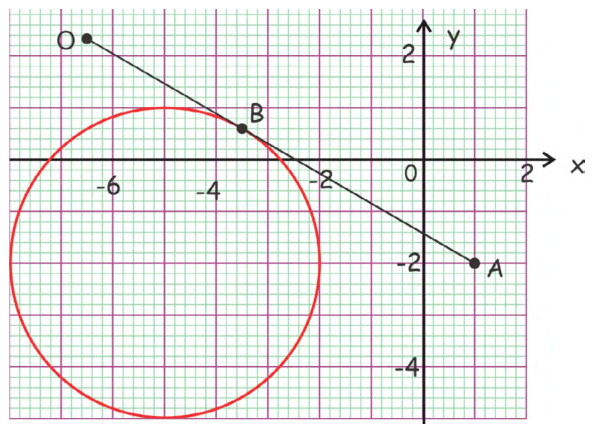
\includegraphics[width=0.5\linewidth]{figures/fig4-26.png}
\end{center}
\figcaption{4.26}{Graph of a circle with Line OBA as tangent}
\begin{enumerate}
  \item[a.] Find the equation of the circle.
  \item[b.] Find $|$AB$|$, leave your answer in surds
\end{enumerate}

\solution
\begin{enumerate}
  \item[a.] The centre of the circle is (-5, -2) and the radius is 3.
  \begin{center}
  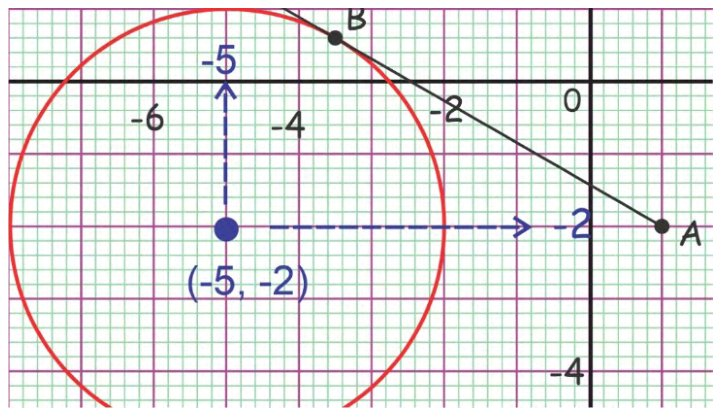
\includegraphics[width=0.6\linewidth]{figures/fig4-27.jpg}
  \end{center}
  \figcaption{4.27}{Graph of a circle with Line OBA as tangent}

  The equation of the circle is: $(x - (-5)^2 + (y - (-2))^2 = 3^2$
  \booknote[S4-12]{a bracket is missing: $(x - (-5))^2$.}
  \begin{align*}
  (x + 5)^2 + (y + 2)^2 &= 9 \\
  x^2 + 10x + 25 + y^2 + 4y + 4 - 9 &= 0 \\
  \boldsymbol{x^2 + y^2 + 10x + 4y - 5} &= \boldsymbol{0}
  \end{align*}
  \item[b.] Coordinates of point A is (1, -2)

  Distance between point A and the centre (-5, -2), $d = \sqrt{(-5 - 1)^2 + (-2 - (-2))^2}$
  \begin{align*}
  d &= \sqrt{(-6)^2 + (0)^2} \\
  d &= \sqrt{36} = 6 \\
  d &= 6
  \end{align*}
  Length of the tangent $= \sqrt{6^2 - 3^2} = \sqrt{36 - 6} = \sqrt{30}$
  \booknote[S4-13]{$3^2 = 9$, not 6: the length is $\sqrt{36 - 9} = \sqrt{27} = 3\sqrt{3}$.}
\end{enumerate}
\end{example}

% Book pp. 166-171 (PDF pp. 167-172)
\section{Deducing the Relation of Various Loci Under Given Condition}

\subsection{Locus}

A locus (plural $=$ loci) is a set of points which satisfies a given condition or
criterion. The result of a locus will either be a complete circle, a part of a circle
(arc), a line or a single point. Here, we will learn about some conditions or criteria
a set of points satisfies.

\textbf{Condition 1:}

The Locus of points are \textbf{equidistant} from one point.

The result of this locus is a circle which will be r units away from the given point.
The given point is the centre of the circle. The criterion or the condition is that:
``it is equidistant from the centre''

Figure 4.28 shows the locus of all points r units from point (h, k)
\begin{center}
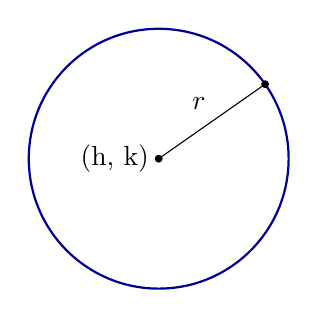
\begin{tikzpicture}[scale=1.1]
  \draw[blue!60!black, thick] (0,0) circle (1.5);
  \fill[black] (0,0) circle (1.3pt);
  \fill[black] (35:1.5) circle (1.3pt);
  \draw[black] (0,0) -- (35:1.5);
  \node[left] at (0,0) {(h, k)};
  \node[above left] at (35:0.8) {$r$};
\end{tikzpicture}
\end{center}
\figcaption{4.28}{Locus of all points r units from point (h, k)}

\begin{example}{Example 4.14}
Find the equation of all points 4 units away from $(-1, 2)$

\solution
This is the same as finding the equation of a circle with centre $(-1, 2)$ and radius
$= 4$.

Using the general equation of the circle, we have:
\booknote[S4-14]{it is the standard equation $(x - h)^2 + (y - k)^2 = r^2$ that is
used here, not the general equation.}
\begin{align*}
(x - (-1))^2 + (y - 2)^2 &= 4^2 \\
(x + 1)^2 + y^2 - 4y + 4 &= 16 \\
x^2 + 2x + 1 + y^2 - 4y + 4 &= 16 \\
x^2 + y^2 + 2x - 4y + 1 + 4 - 16 &= 0
\end{align*}
$\boldsymbol{x^2 + y^2 + 2x - 4y - 11 = 0}$ is the locus of all points 4 units away from the point
$(-1, 2)$
\end{example}

\textbf{Condition 2:}

The locus of points equidistant from two fixed points.

The result of this locus is a line which will perpendicularly bisect the line joining
the two points.

Figure 4.29 below shows the locus of points, L, equidistant from points P and Q.
Line L bisects PQ perpendicularly at m, the midpoint of line PQ.
\begin{center}
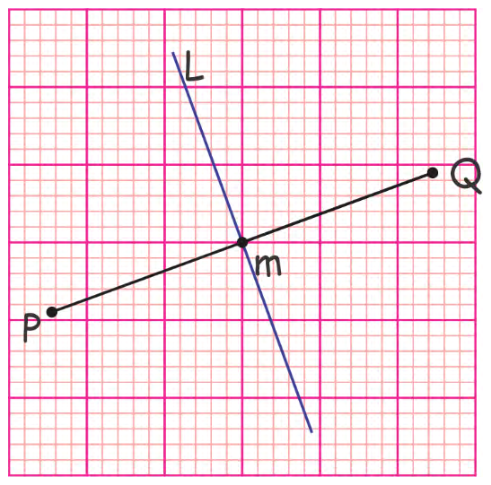
\includegraphics[width=0.4\linewidth]{figures/fig4-29.png}
\end{center}
\figcaption{4.29}{Locus of points, L, equidistant from points P and Q}

\begin{example}{Example 4.15}
Calculate the equation of all points equidistant from A(-5, 0) and B(3, -6)

\solution
\begin{align*}
\text{Midpoint of line AB} &= \left(\frac{-5 + 3}{2}, \frac{0 + -6}{2}\right) \\
&= \left(-\frac{2}{2}, -\frac{6}{2}\right) \\
&= (-1, -3)
\end{align*}
\begin{align*}
\text{Gradient of line AB} &= \frac{-6 - 0}{3 \text{ --- } 5} \\
&= -\frac{6}{8} \\
&= -\frac{3}{4}
\end{align*}
\begin{align*}
\text{Gradient of the locus} &= -1 \div \left(-\frac{3}{4}\right) \\
&= -1 \times -\frac{4}{3} \\
&= \frac{4}{3}
\end{align*}
Equation of the locos is:
\begin{align*}
y - -3 &= \frac{4}{3}(x - (-1)) \\
y + 3 &= \frac{4}{3}(x + 1)
\end{align*}
Multiply through by 3:
\begin{align*}
3 \times (y + 3) &= 3 \times \frac{3}{4}(x + 1) \\
3y + 9 &= 4(x + 1) \\
3y + 9 &= 4x + 4 \\
3y - 4x + 9 - 4 &= 0 \\
3y - 4x + 5 &= 0
\end{align*}
Therefore, $3\boldsymbol{y} - 4\boldsymbol{x} + 5 = 0$ is the locus of all points equidistant from (-5, 0) and
(3, -6)
\end{example}

\textbf{Condition 3:}

The locus of points equidistant from two intersecting lines.

The result of this locus is a pair of angle bisectors. For any point (x, y) on the
angle bisector, the perpendicular distance is equidistant from the two lines.

In Figure 4.30, l and m are the loci equidistant from line AB and line CD.

Line L bisects angle BOD and M bisects angle AOD.

Also, for any point P(x, y) on the locus, L, the perpendicular distance between
point P and line AB is equal to the perpendicular distance between point P and
line CD.
\begin{center}
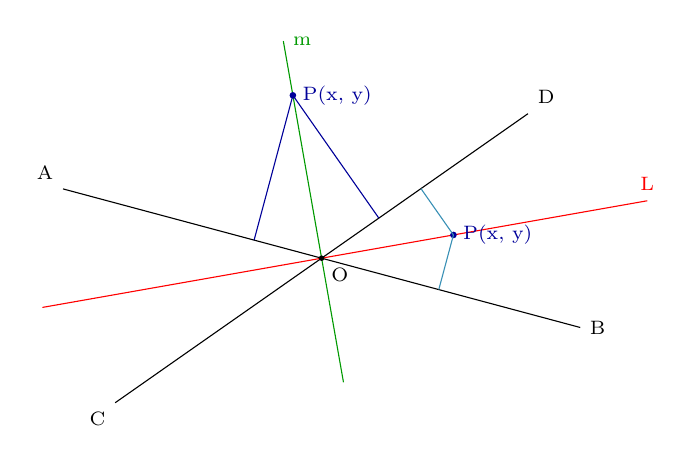
\begin{tikzpicture}[scale=1.0, font=\scriptsize]
  \coordinate (O) at (0,0);
  % line AB: direction 165 deg (A upper left) to -15 deg (B lower right)
  \draw[black] (165:3.4) node[above left] {A} -- (-15:3.4) node[right] {B};
  % line CD: direction 215 deg (C lower left) to 35 deg (D upper right)
  \draw[black] (215:3.2) node[below left] {C} -- (35:3.2) node[above right] {D};
  % bisector L of angle BOD: direction 10 deg
  \draw[red] (190:3.6) -- (10:4.2) node[above] {L};
  % bisector m of angle AOD: direction 100 deg
  \draw[green!60!black] (280:1.6) -- (100:2.8) node[right] {m};
  \fill[black] (O) circle (1pt);
  \node[below right] at (O) {O};
  % P on m
  \coordinate (P1) at (100:2.1);
  \fill[blue!60!black] (P1) circle (1.2pt);
  \node[blue!60!black, right] at (P1) {P(x, y)};
  \draw[blue!60!black] (P1) -- ($(165:3.4)!(P1)!(-15:3.4)$);
  \draw[blue!60!black] (P1) -- ($(215:3.2)!(P1)!(35:3.2)$);
  % P on L
  \coordinate (P2) at (10:1.7);
  \fill[blue!60!black] (P2) circle (1.2pt);
  \node[blue!60!black, right] at (P2) {P(x, y)};
  \draw[cyan!70!black] (P2) -- ($(165:3.4)!(P2)!(-15:3.4)$);
  \draw[cyan!70!black] (P2) -- ($(215:3.2)!(P2)!(35:3.2)$);
\end{tikzpicture}
\end{center}
\figcaption{4.30}{Locus of points equidistant from two intersecting lines}

\begin{example}{Example 4.16}
Find the equation of the locus of points which moves so that its distance from the
lines

$y = 2x - 3$ and $x + 2y = 5$ is the same.

Let P(x, y) be any point on the loci. This means that the perpendicular distance
between P(x, y) and the line $y = 2x - 3$ is equal to the perpendicular distance
between point P(x,y) and the line $x + 2y = 5$

Recall that the perpendicular distance between a point (m,n) and a line $ax + by
+ c = 0$ is
\[ \left|\frac{a(m) + b(n) + c}{\sqrt{a^2 + b^2}}\right| \]
The equation of the loci is given by:
\begin{align*}
\left|\frac{y - 2x + 3}{\sqrt{1^2 + (-2)^2}}\right| &= \left|\frac{2y + x - 5}{\sqrt{2^2 + 1^2}}\right| \\
\left|\frac{y - 2x + 3}{\sqrt{5}}\right| &= \left|\frac{2y + x - 5}{\sqrt{5}}\right|
\end{align*}
multiply both sides by $\sqrt{5}$,which effectively removes the denominator:
\[ |y - 2x + 3| = |2y + x - 5| \]
Remove the absolute value sign by multiplying \textbf{any side} of the equation by $\pm$

In this example, we chose to remove the absolute value sign by multiplying the
RHS of the equation by $\pm$
\[ y - 2x + 3 = \pm(2y + x - 5) \]
So, either
\begin{center}
\begin{tabular}{@{}l@{\qquad}c@{\qquad}l@{}}
$y - 2x + 3 = 2y + x - 5$ & or & $y - 2x + 3 = -2y - x + 5$ \\
$0 = 2y - y + x + 2x - 5 - 3$ & & $y + 2y - 2x + x + 3 - 5 = 0$ \\
$y + 3x - 8 = 0$ & & $3y - x - 2 = 0$
\end{tabular}
\end{center}
Therefore, the equation of the locus is either $\boldsymbol{y} + 3\boldsymbol{x} - 8 = 0$ \textbf{or} $3\boldsymbol{y} - \boldsymbol{x} - 2 = 0$
\end{example}

\textbf{Condition 4:}

The locus equidistant from a line.

The result of this locus is a pair of lines equidistant from the given line.

For instance, the locus of points $\boldsymbol{d}$ units away from line AB is either line M or line
L as shown in Figure 4.31.
\begin{center}
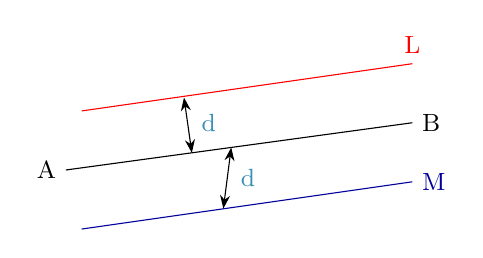
\begin{tikzpicture}[scale=1.0, font=\small]
  \draw[black] (-2.2,-0.3) node[left] {A} -- (2.2,0.3) node[right] {B};
  \draw[red] (-2.0,0.45) -- (2.2,1.05) node[above] {L};
  \draw[blue!60!black] (-2.0,-1.05) -- (2.2,-0.45) node[right] {M};
  \draw[{Stealth}-{Stealth}] (-0.6,-0.083) -- (-0.7,0.62);
  \draw[{Stealth}-{Stealth}] (-0.1,-0.014) -- (-0.2,-0.79);
  \node[cyan!70!black, right] at (-0.6,0.3) {d};
  \node[cyan!70!black, right] at (-0.1,-0.4) {d};
\end{tikzpicture}
\end{center}
\figcaption{4.31}{Locus equidistant from a line}

So, if the equation of AB is $ax + by + c = 0$, then $d = \left|\dfrac{ax + by + c}{\sqrt{a^2 + b^2}}\right|$

\begin{example}{Example 4.17}
Find the locus of the point R(x, y) such that it is always 3 units from the line $y + 1 = 0$

\solution
\begin{align*}
3 &= \left|\frac{0x + y + 1}{\sqrt{0^2 + 1^2}}\right| \\
3 &= \left|\frac{y + 1}{\sqrt{1}}\right| \\
3 &= \pm|y + 1| \\
3 &= y + 1 \text{ or } 3 = -y - 1 \\
y - 2 &= 0 \text{ or } y + 4 = 0
\end{align*}
Therefore, the locus R($x$, $y$) of points which is 3 units away from $y + 1 = 0$ is
either $\boldsymbol{y} - 2 = 0$ \textbf{or} $\boldsymbol{y} + 4 = 0$
\end{example}

\begin{example}{Example 4.18}
If P(1, 4) and Q(5, -1) are two fixed points and A(x,y) moves such that $|$AP$|$:$|$AQ$|$
$= 1$:2. Find the equation of the locus.

\solution
From the condition given, $|$AP$|$:$|$AQ$| = 1 : 2$
\begin{align*}
\frac{|AP|}{|AQ|} &= \frac{1}{2} \\
2|AP| &= 1 \times |AQ| \\
2\sqrt{(y - 4)^2 + (x - 1)^2} &= \sqrt{(y - (-1))^2 + (x - 5)^2} \\
2\sqrt{(y - 4)^2 + (x - 1)^2} &= \sqrt{(y + 1)^2 + (x - 5)^2}
\end{align*}
Square both sides:
\begin{align*}
4\left[y^2 - 8y + 16 + x^2 - 2x + 1\right] &= y^2 + 2y + 1 + x^2 - 10x + 25 \\
4y^2 - 32y + 64 + 4x^2 - 8x + 4 &= y^2 + 2y + 1 + x^2 - 10x + 25 \\
4y^2 - y^2 - 32y - 2y + 4x^2 - x^2 - 8x + 10x + 68 - 26 &= 0
\end{align*}
$3\boldsymbol{x}^2 + 3\boldsymbol{y}^2 + 2\boldsymbol{x} - 34\boldsymbol{y} + 42 = 0$ is the equation of the locus.
\end{example}

\begin{example}{Example 4.19}
A point A(x, y) moves such that AC and AD are perpendicular.

If C(-3, 0) and D(3, 5), find the equation of the locus A.

\solution
Since AC and AD are perpendicular, (gradient of AC)$\times$ (gradient of AD)$= -1$
\begin{align*}
\left(\frac{y - 0}{x - (-3)}\right) \times \left(\frac{y - 5}{x - 3}\right) &= -1 \\
\left(\frac{y}{x + 3}\right) \times \left(\frac{y - 5}{x - 3}\right) &= -1 \\
\frac{y^2 - 5y}{x^2 - 9} &= -\frac{1}{1}
\end{align*}
Cross multiply:
\begin{align*}
y^2 - 5y &= -1(x^2 - 9) \\
y^2 - 5y &= -x^2 + 9
\end{align*}
$\boldsymbol{y^2 + x^2 - 5y - 9 = 0}$ is the locus A
\end{example}

\section{Extended Reading}
\begin{itemize}
  \item Mathematical Association of Ghana (2009). Effective Elective Mathematics:
  Seddco Publishing Limited. ISBN 978 9964 72 4740.
\end{itemize}

% Book pp. 172-175 (PDF pp. 173-176).  The numbering is the book's own.
\section*{Review Questions}
\booknote[S4-15]{the book numbers the questions 1 to 25, but several single
problems are split over two numbers (1/2, 6/7, 10/11, 12/13, 14/15 and 24/25),
and question 1 g is the last sentence of 1 f. The answer key numbers the same
problems 1 to 19.}

\begin{enumerate}[leftmargin=*, widest=25]
\item[1.] The diagram below shows the graph of three circles, P, Q and R.
\item[2.] Use it to answer the questions\textbf{.}
\begin{center}
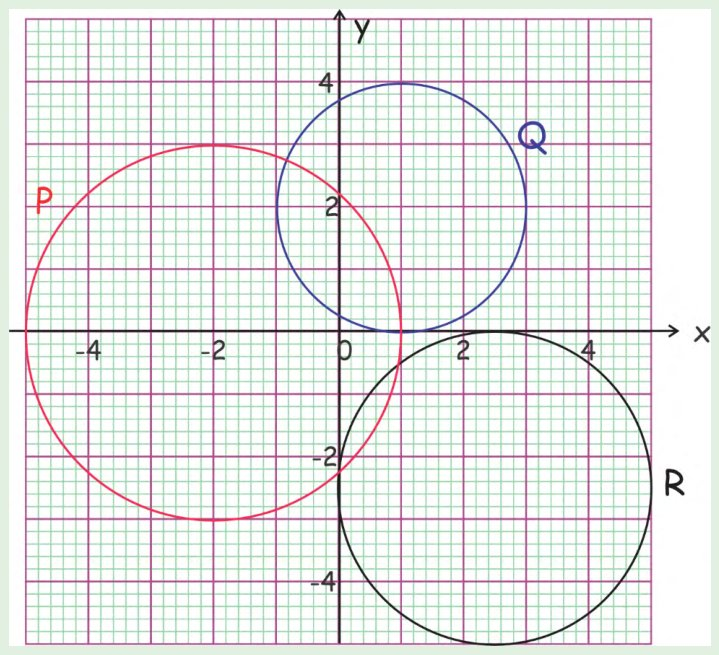
\includegraphics[width=0.6\linewidth]{figures/rq4-1.jpg}
\end{center}
\begin{enumerate}
  \item[a.] State the coordinates of the centre of P, Q and R.
  \item[b.] Find the radii of circles P, Q and R
  \item[c.] Write the equation of circle R in general form
  \item[d.] Write the equation of circle P in the standard form
  \item[e.] Write the equation of circle Q in the standard form
  \item[f.] Find the perimeter of the triangle formed by the centres of the three
  circles.
  \item[g.] Give your answer correct to three significant figures.
\end{enumerate}

\item[3.] Write the general form of the circle equation with the following properties.
\begin{enumerate}
  \item[a.] Centre (1, -1) and radius 7
  \item[b.] Centre (-2, 1) and radius 5
  \item[c.] Centre (0, -3) and radius 2
  \item[d.] Centre (-3, -4) and radius 8
\end{enumerate}

\item[4.] The diagram shows the graph of circles A, B and C.

Use them to answer the following questions.
\begin{center}
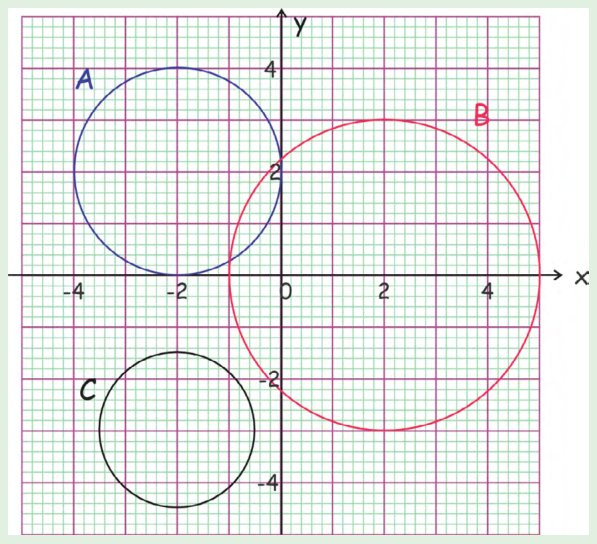
\includegraphics[width=0.5\linewidth]{figures/rq4-4.jpg}
\end{center}
\begin{enumerate}
  \item[a.] Write the equation of each circle in the general form
  \item[b.] Find the perimeter of the triangle formed by the centres of the circle.
  Leave your answer in surd form.
\end{enumerate}

\item[5.] A TV remote has a range of 8m in all directions. If the TV is 5m East and
3m South, write an equation to represent the area within which the TV
receives signals from the remote. Can the TV receive signals from the
remote if the remote is located 2m West? Justify your response.

\item[6.] An Uber driver operates within 30km of a post office at all angles. His
house is 5km West and 12km south of a post office.
\item[7.] \mbox{}
\begin{enumerate}
  \item[a.] Write an equation to represent the driver's travel boundary from the
  post office using the driver's house as the origin. Leave your equation
  in standard form.
  \item[b.] Find the furthest distance between the driver's house and his travel
  boundary.
  \item[c.] Find the shortest distance between the driver's house and the driver's
  travel boundary.
\end{enumerate}

\item[8.] Write the general equation of a circle with:
\begin{enumerate}
  \item[a.] Centre $(4, -1)$ and radius $\sqrt{11}$.
  \item[b.] Centre $(-2, -3)$ and radius $2\frac{1}{2}$
  \item[c.] Centre $(0, -3)$ and radius $\frac{1}{3}$
  \item[d.] Centre $\left(\frac{1}{2}, -1\right)$ and radius $1\frac{1}{2}$
\end{enumerate}

\item[9.] Write each of the following circles in the standard form. Also, state the
centre and radius of each circle.
\begin{enumerate}
  \item[a.] $x^2 + y^2 - 2x + 2y - 47 = 0$
  \item[b.] $x^2 + y^2 + 6y = 0$
  \item[c.] $x^2 + y^2 - 12x - 64 = 0$
  \item[d.] $x^2 + y^2 + 4x - 8y + 4 = 0$
  \item[e.] $2x^2 + 2y^2 - 2x - 2y - 7 = 0$
  \item[f.] $3x^2 + 3y^2 + 12x - 2y + 4 = 0$
\end{enumerate}

\item[10.] The endpoints of the diameter of a circle are (0, 5) and (0, -7).
\item[11.] Find the
\begin{enumerate}
  \item[a.] radius and centre of the circle
  \item[b.] general equation of the circle.
\end{enumerate}

\item[12.] The endpoints of the diameter of a circle are (6, 0) and (-2, 0).
\item[13.] Find the
\begin{enumerate}
  \item[a.] radius and centre of the circle
  \item[b.] general equation of the circle.
\end{enumerate}

\item[14.] The endpoints of the diameter of a circle are (-4, 3) and (4, -3).
\item[15.] Find the
\begin{enumerate}
  \item[a.] radius and centre of the circle
  \item[b.] general equation of the circle.
\end{enumerate}

\item[16.] In each of the following questions, coordinates of three points are provided.
Write the general equation of the circle that satisfies all three points. State
the centre and radius of the resulting circle.
\begin{enumerate}
  \item[a.] $(-5, 0)$, $(-1, -4)$ and $(-1, 4)$
  \item[b.] $(6, -1)$, $(3, -4)$ and $(0, -1)$
\end{enumerate}

\item[17.] Find the equations of the line tangent and normal to the circle.
\begin{enumerate}
  \item[a.] $x^2 + y^2 = 100$ at point $(-8, -6)$
  \item[b.] $x^2 + y^2 = 49$ at point (7, 0)
  \item[c.] $x^2 + y^2 - 2x - 24 = 0$ at (1, -5)
\end{enumerate}

\item[18.] Find the length of the tangent from the point:
\begin{enumerate}
  \item[a.] (-8, 6) to the circle $x^2 + y^2 - 25 = 0$, leave your answer in surd form
  \item[b.] (3, 6) to the circle $x^2 + y^2 - 4y - 5 = 0$
  \item[c.] $(7, -3)$ to the circle $x^2 + y^2 + 10x - 4y + 13 = 0$, leave your answer
  in surd form
  \item[d.] $\left(5, -\frac{1}{2}\right)$ to the circle $4x^2 + 4y^2 + 12x + 4y - 15 = 0$
\end{enumerate}

\item[19.] The diagram below shows a graph of a circle. Line BA is a tangent to the
circle at B.
\begin{center}
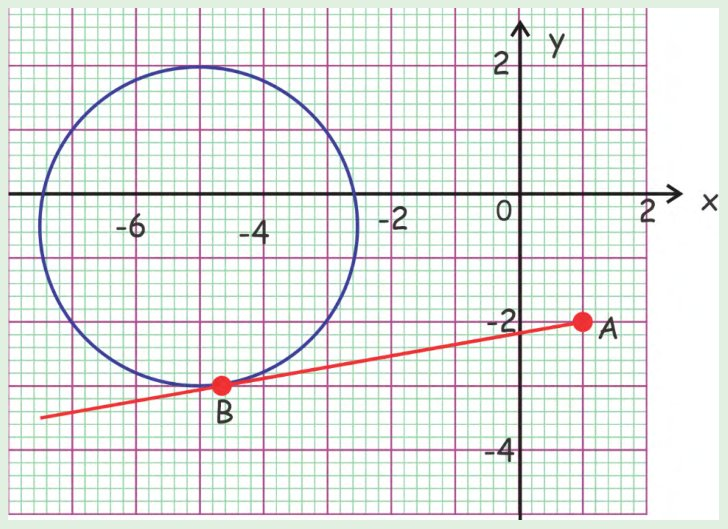
\includegraphics[width=0.6\linewidth]{figures/rq4-19.jpg}
\end{center}
\begin{enumerate}
  \item[a.] Find the equation of the circle.
  \item[b.] Find $|$AB$|$, leave your answer in surds
\end{enumerate}

\item[20.] Calculate the equation of all points equidistant from A(-4, 0) and B(2, 8))

\item[21.] Find the equation of the locus of points which moves so that its distance
from the lines $3y - x = 0$ and $x - 3y = 0$ is the same.
\booknote[S4-16]{$3y - x = 0$ and $x - 3y = 0$ are the same line, so as printed
the question has no meaningful answer; the answer key gives $y - x = 0$.}

\item[22.] Find the locus of point R(x, y) that is always 2 units from the line $x + 5 =
0$

\item[23.] If P(-2, 1) and Q(4, -1) are two fixed points and A($x$, $y$) moves such that
$|$AP$|$:$|$AQ$| = 2$:1. Find the equation of the locus\textbf{.}

\item[24.] A point A($x$, $y$) moves so that AC and AD are perpendicular. C(-2, 0) and
D(6, 4).
\item[25.] Find the equation of the locus A.
\end{enumerate}


% Sections 5-14: not yet transcribed.

\chapter*{Answers to Review Questions}
\addcontentsline{toc}{chapter}{Answers to Review Questions}
\markboth{ANSWERS TO REVIEW QUESTIONS}{}

\section*{Review Questions for Section 1}
% Answers to the Section 1 Review Questions, book pp. 448-452 (PDF pp. 449-453).
% Added 2026-09-04 (not part of the original Section 1 transcription); the numbering and
% wording are the answer key's own.  Venn diagrams are cropped from the PDF into
% figures/ans-*.png.
\noindent\textbf{Part A}
\begin{enumerate}
\item
\begin{enumerate}
  \item[a.] A $= \{2, 4, 5, 6, 7, 9, 11, 12, 13, 15, 18, 20, 23, 29\}$

  B $= \{2, 3, 5, 7, 11, 13, 17, 19, 23, 29\}$

  C $= \{1, 3, 5, 7, 9, 11, 13, 15, 17\}$
  \item[b.] $A' = \{1, 3, 8, 10, 16, 17, 19\}$

  $B' = \{1, 4, 6, 8, 9, 10, 12, 15, 16, 18, 20\}$

  $C' = \{2, 4, 6, 8, 10, 12, 16, 18, 19, 20, 23, 29\}$
  \item[c.] (i) $= \{8, 10, 16\}$

  (ii) $= \{8, 10, 16\}$

  (iii) $= \{1, 2, 3, 4, 6, 8, 9, 10, 12, 15, 16, 17, 18, 19, 20, 23, 29\}$

  (iv) $= \{1, 2, 3, 4, 6, 8, 9, 10, 12, 15, 16, 17, 18, 19, 20, 23, 29\}$
  \item[d.] $(A \cup B \cup C)' = A' \cap B' \cap C'$
  \item[e.] $(A \cap B \cap C)' = A' \cup B' \cup C'$
  \item[f.] A set of prime numbers less than 30
  \item[g.] A set of odd numbers less than 18
\end{enumerate}

\item
\begin{enumerate}
  \item[a.] G $= \{$a, e, i, o, u, n, r, d, m, y, t, h, p$\}$

  E $= \{$a, e, i, o, u, d, m, y, t, h, p, c, l, s$\}$

  T $= \{$a, e, i, o, u, n, s, b, f, g, k, v$\}$

  $\varepsilon = \{$a, e, i, o, u, n, r, d, m, y, t, h, p, c, l, s, b, f, g, k, v, w, x, z$\}$
  \item[b.] $G' \cap E' = \{b, f, g, k, v, w, x, z\} = (G \cup E)'$
  \item[c.] $(G \cap E \cap T)' = \{$n, r, d, m, y, t, h, p, c, l, s, b, f, g, k, v, w, x, z$\}$
  $= G' \cup E' \cup T'$
  \item[d.] $(G \cup E \cup T)' = \{w, x, z\} = G' \cap E' \cap T'$
\end{enumerate}

\item B
\item A
\item D
\item A
\item B
\item (i) $R' \cap S$ \quad (ii) $M \cup N'$ \quad (iii) $(A' \cup B) \cup C'$ \quad
(iv) $\{\ \}$ or $\phi$ \quad (v) $A' \cup B$
\item
\begin{enumerate}
  \item[(a)] $[(R \cup M)' \cap P]' = R' \cap M' \cap B = R \cup M \cup P'$
  \item[(b)] $[(R \cap M) \cup M']' = R' \cap M$
\end{enumerate}
\booknote{the middle expression of 9(a) is printed as in the book; the complement of
$(R \cup M)' \cap P$ is $R \cup M \cup P'$.}

\item
\begin{enumerate}
  \item[a.]\leavevmode\par\nopagebreak\begin{center}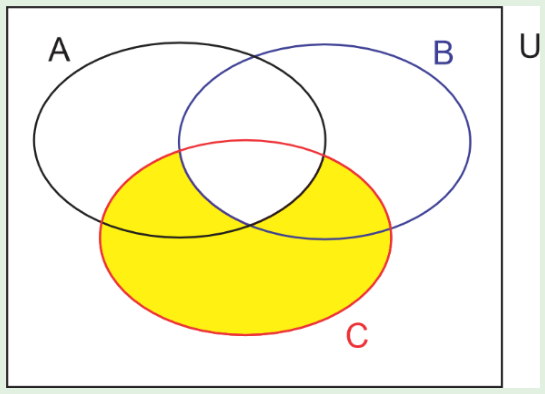
\includegraphics[width=0.45\linewidth]{figures/ans-q10a.png}\end{center}
  \item[b.]\leavevmode\par\nopagebreak\begin{center}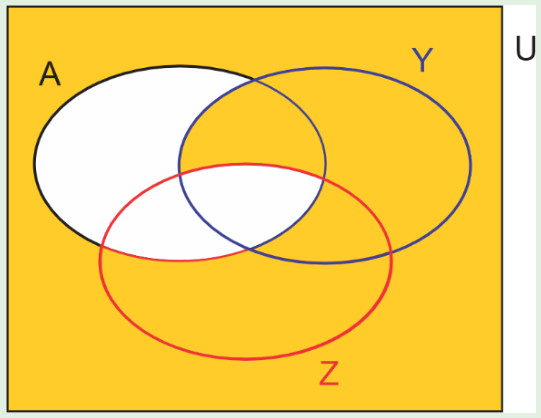
\includegraphics[width=0.45\linewidth]{figures/ans-q10b.png}\end{center}
\end{enumerate}

\item
\begin{enumerate}
  \item[a.] (i) X $= \{2, 3, 5, 7, 11, 13, 17, 19\}$

  (ii) Y $= \{1, 2, 3, 4, 5, 6, 7, 8, 9, 10, 11\}$

  (iii) X $\cap\, Y \cap Z = \{2, 3, 5, 7\}$

  (iv) $X \cup Y' = \{0, 2, 3, 5, 7, 11, 12, 13, 14, 15, 16, 17, 18, 19, 21\}$

  (v) $(X \cup Y) \cap Z' = \{8, 9, 10, 11, 17, 19\}$

  (vi) $(X' \cap Y) \cup Z = \{1, 2, 3, 4, 5, 6, 8, 9, 10, 14, 15, 16, 18\}$
  \item[b.]\leavevmode\par\nopagebreak\begin{center}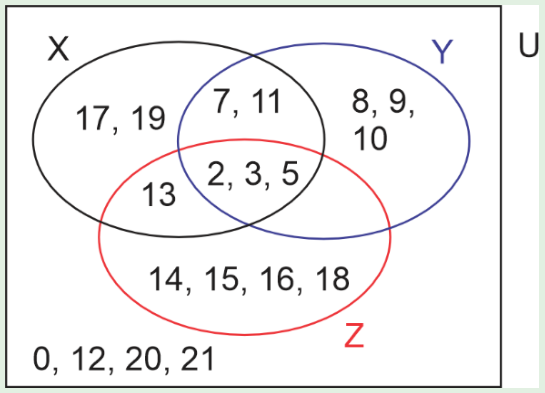
\includegraphics[width=0.5\linewidth]{figures/ans-q11b.png}\end{center}
\end{enumerate}

\item
\begin{enumerate}
  \item[a.]\leavevmode\par\nopagebreak\begin{center}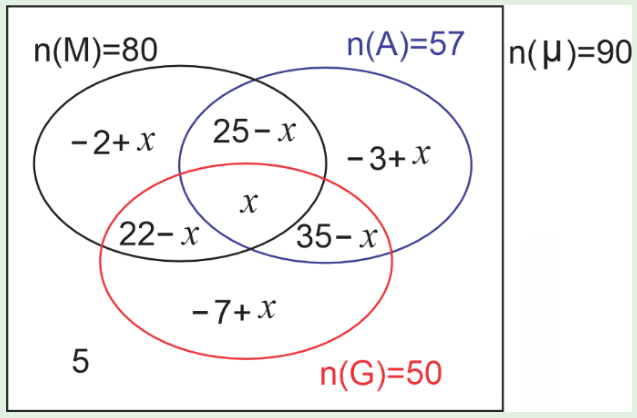
\includegraphics[width=0.55\linewidth]{figures/ans-q12a.png}\end{center}
  \item[b.] Solving it $x = 15$, so the number who only teach one subject is
  $13 + 12 + 8 = 33$
\end{enumerate}

\item
\begin{enumerate}
  \item[a.] 7
  \item[b.] 17
\end{enumerate}

\item
\begin{enumerate}
  \item[a.] (i) 10 \quad (ii) 4 \quad (iii) 32
  \item[b.] Probability $= \dfrac{40}{60} = \dfrac{2}{3}$
\end{enumerate}

\item
\begin{enumerate}
  \item[a.] 3\% \quad b. 2\%
  \item[c.] 15\% \quad d. 13\%
  \item[e.] 5\%
\end{enumerate}

\item
\begin{enumerate}
  \item[a.] 320
  \item[b.] (i) 176 \quad (ii) 16 \quad (iii) 124
\end{enumerate}

\item a. 24 \quad b. 77
\item a. 35 \quad b. 20

\item
\begin{enumerate}
  \item[a.]\leavevmode\par\nopagebreak\begin{center}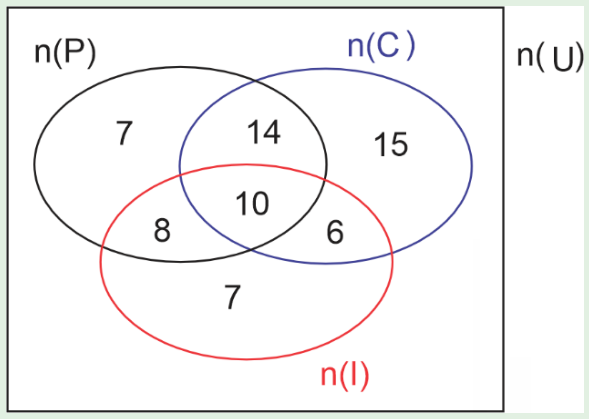
\includegraphics[width=0.5\linewidth]{figures/ans-q19a.png}\end{center}
  \item[b.] 67
  \item[c.] 29
\end{enumerate}
\end{enumerate}

\noindent\textbf{Part B}
\begin{enumerate}
\item
\begin{enumerate}
  \item[a.] $1 + 48x + 1056x^2 + 14080x^3 + 126720x^4$
  \item[b.] $1 - 27x + 324x^2 - 2268x^3 + 10260x^4$
  \item[c.] $2187 + 10206x + 20412x^2 + 22680x^3 + 15120x^4$
  \item[d.] $1 - 4x + 7x^2 - 7x^3 + \dfrac{35}{8}x^4$
  \item[e.] $64 - 480x + 1500x^2 - 2500x^3 + \dfrac{9375}{4}x^4$
\end{enumerate}

\item
\begin{enumerate}
  \item[a.] $135x^2$
  \item[b.] $\dfrac{12920}{243}x^6$
  \item[c.] $32\,440\,320\,a^4 b^8$
\end{enumerate}

\item
\begin{enumerate}
  \item[a.] $1 + 6x + 12x^2$
  \item[b.] $2 + 63x + 1000x^2$
  \item[c.] $5 - 38x + \dfrac{392}{3}x^2$
  \item[d.] $1 - 56x + 1470x^2$
\end{enumerate}

\item $(1 - 2x)^7 \approx 1 - 14x + 84x^2 - \ldots$, so when $x = 0.01$, $(0.98)^7 \approx 0.8684$

\item
\begin{enumerate}
  \item[a.] $\left(1 - \dfrac{1}{2}x\right)^{\frac{1}{2}} = 1 - \dfrac{1}{4}x - \dfrac{1}{32}x^2 + \dfrac{1}{128}x^3 + \ldots$
  \item[b.] $(1 - 2x)^{-3} = 1 + 6x + 6x^2 + 80x^3 + \ldots$
  \item[c.] $(3 - x)^{-2} = \dfrac{1}{9} + \dfrac{2}{27}x + \dfrac{x^2}{27} + \dfrac{4}{243}x^3 + \ldots$
\end{enumerate}
\booknote{5(b) is printed as in the book; the $x^2$ coefficient of $(1-2x)^{-3}$ is 24.}

\item
\begin{enumerate}
  \item[a.] 2.0567 \quad b. 3.0015
  \item[c.] 2.005 \quad d. 0.3162
  \item[e.] 10.0499 \quad f. 0.9752
\end{enumerate}

\item Expand $(1 - x)^{\frac{1}{3}}$ to the $x^3$ term; also expand $(1 + x)^{-\frac{1}{3}}$ to $x^3$.
Then multiply the results to obtain $1 - \dfrac{2}{3}x + \dfrac{2}{9}x^2 - \dfrac{4}{21}x^3 \ldots$

\item
\begin{enumerate}
  \item[a.] $1 + 3x + 9x^2 + 13x^3$
  \item[b.] $1 + 12x + 58x^2 + 144x^3$
\end{enumerate}

\item
\begin{enumerate}
  \item[a.] $1 + 9py + 36p^2y^2$
  \item[b.] $p = 4$, $q = 576$
\end{enumerate}

\item a. $128 + 448kx + 672k^2x^2$ \quad b. $k = 4$
\end{enumerate}


\section*{Review Questions for Section 2}
% Answers to the Section 2 Review Questions, book pp. 452-453 (PDF pp. 453-454).
% The answer key numbers its entries 1-16 against the 19 printed questions:
% answer 13 covers Q13/14, answer 14 is Q15, answer 15 covers Q16-18, answer 16
% is Q19.  The numbering below is the answer key's own.
\begin{enumerate}
\item $a = 1$, $r = 2$
\item
\begin{enumerate}
  \item[a.] (i) 29, 33, 37 \quad (ii) $21 + 4n$
  \item[b.] $n(23 + 2n)$, 430
\end{enumerate}
\item $4, -1, -6$
\item (i) $\dfrac{15}{8}$ \quad (ii) 2
\item $\dfrac{1}{162}$
\item (i) 2, 3, 5, 9, 17
\item $a = -2$ and $d = -3$
\item (i) \cedi\ 4,500,000.00 \quad (ii) \cedi\ 4,812,000.00
\item 3, 5, 7 and $U_n = 2n + 1$
\item (i) $\left(\dfrac{1}{3}\right)^3 h$ \quad (ii) $\left(\dfrac{1}{3}\right)^n h$
\item 3
\item 79
\item 20 shirts and 100 pairs of trousers.
\item
\begin{enumerate}
  \item[a.] $x \le -2$, $x \ge \dfrac{1}{3}$
  \item[b.] $x \le -1$, $x \ge 3$.
\end{enumerate}
\item The company should produce and sell at least 190 bags of maize.
\item
\begin{enumerate}
  \item[a.] $18h + 36t \le 150$, $15h + 30t \le 85$, $h \ge 0$, $t \ge 0$
  \item[b.] $0 \le h \le \dfrac{17}{3}$
\end{enumerate}
\end{enumerate}


\section*{Review Questions for Section 3}
% Answers to the Section 3 Review Questions, book pp. 453-456 (PDF pp. 454-457).
% The answer key's own numbering, which matches the 14 printed questions.
\begin{enumerate}
\item
\begin{enumerate}
  \item[a.] $x = 3, -\frac{1}{3}, -\frac{1}{2}$
  \item[b.] $x = 1, -\frac{2}{5}, -1$
\end{enumerate}
\item
\begin{enumerate}
  \item[a.] the zeros are -1, 0.5. and 3
  \item[b.] the factors are $(x + 1)\,(2x\text{-}1)\,(x\text{-}3)$
  \item[c.] --1 $>$ x, --1 $<$ x $<$ 0.5, 0.5 $<$ x $<$ 3, x $>$ 3
  \item[d.] $f(x) = 2x^3 - 5x^2 - 4x + 3$
\end{enumerate}
\item
\begin{enumerate}
  \item[a.] \mbox{}\par\nopagebreak
  \begin{center}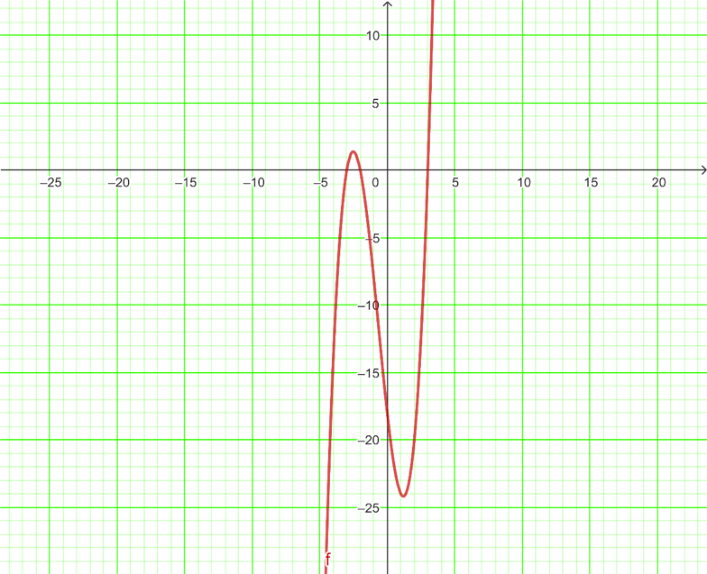
\includegraphics[width=0.55\linewidth]{figures/ans3-3a.png}\end{center}
  \item[b.] \mbox{}\par\nopagebreak
  \begin{center}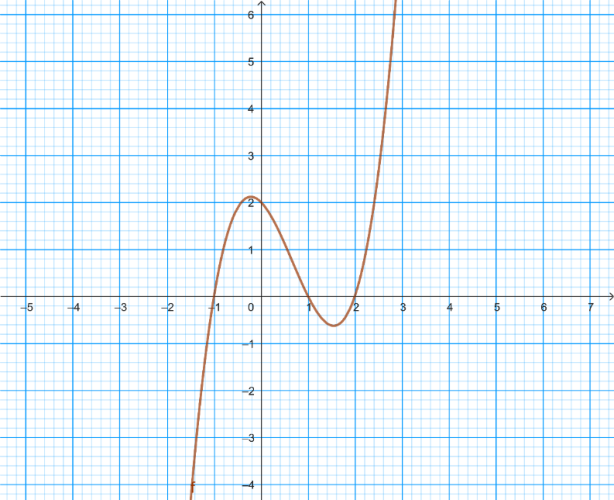
\includegraphics[width=0.55\linewidth]{figures/ans3-3b.png}\end{center}
  \item[c.] \mbox{}\par\nopagebreak
  \begin{center}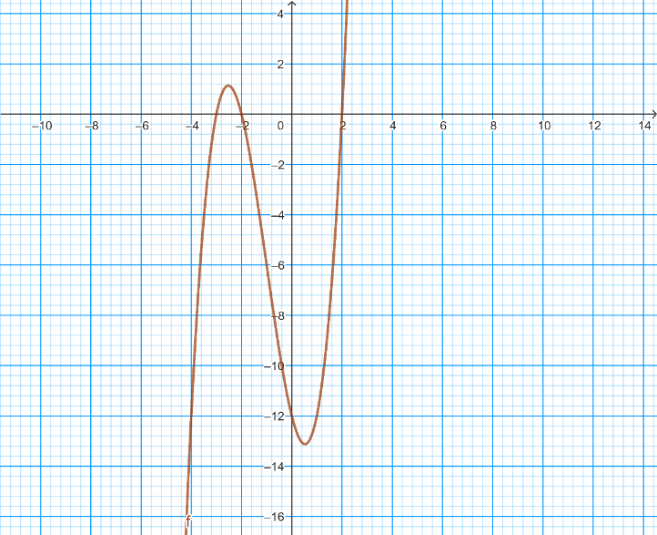
\includegraphics[width=0.55\linewidth]{figures/ans3-3c.png}\end{center}
  \item[d.] \mbox{}\par\nopagebreak
  \begin{center}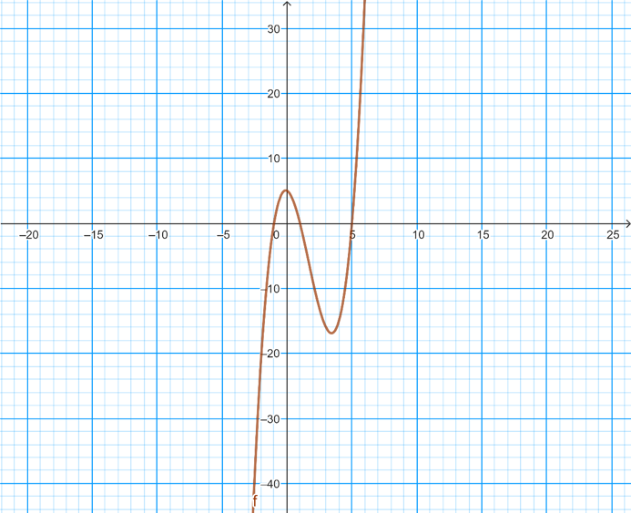
\includegraphics[width=0.55\linewidth]{figures/ans3-3d.png}\end{center}
  \item[e.] \mbox{}\par\nopagebreak
  \begin{center}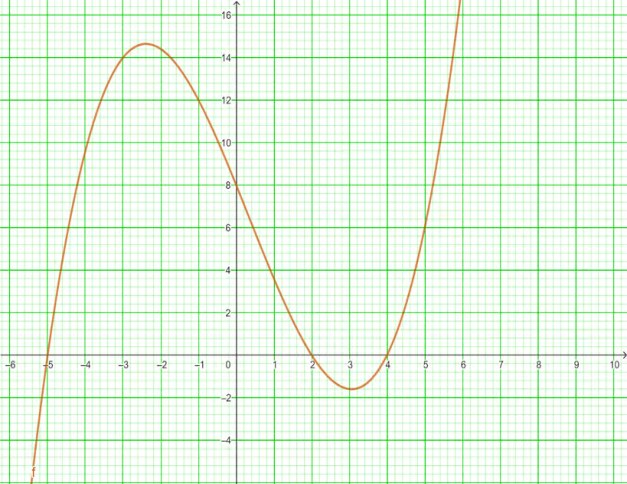
\includegraphics[width=0.55\linewidth]{figures/ans3-3e.jpg}\end{center}
\end{enumerate}
\item
\begin{enumerate}
  \item[a.] $(x - 1)(x + 2)(x + 4)$
  \item[b.] $(x + 2)(2x + 5)(x - 3)$
  \item[c.] $(x - 2)(2x -\ )(2x)$
  \booknote[S3-17]{the answer is garbled; $4x^3 - 4x^2 - 11x + 6 = (x - 2)(2x + 3)(2x - 1)$.}
  \item[d.] $(x + 2)(3x + 2)(2x - 1)$
  \item[e.] $(x - 1)(3x + 1)(x + 6)$
\end{enumerate}
\item
\begin{enumerate}
  \item[a.] $x = 1, -3, -2$
  \item[b.] $x = -5, 1, 0.5$
  \item[c.] $x = -2, 1, 0.5$
  \item[d.] $x = -1.5, 1.5, 2$
  \item[e.] $x = -0.5, 1, 0.5$
  \item[f.] $x = 1, 0.5, 1.5$
\end{enumerate}
\item
\begin{enumerate}
  \item[a.] $0, i\sqrt{6}, -i\sqrt{6}$
  \item[b.] $i\sqrt{\frac{7}{2}}, -i\sqrt{\frac{7}{2}}, -\sqrt{5}, \sqrt{5}$
  \booknote[S3-18]{$2x^4 + 17x^2 + 35 = (2x^2 + 7)(x^2 + 5)$, so the last two roots
  are $-i\sqrt{5}$ and $i\sqrt{5}$.}
  \item[c.] $-\sqrt{7 + \sqrt{13}},\ ,\ \sqrt{7 + \sqrt{13}}, -\sqrt{7 - \sqrt{13}},
  \sqrt{7 - \sqrt{13}}$
  \item[d.] $1, -1, i, -i$
  \item[e.] $0, 3i\sqrt{3}, -3i\sqrt{3}$
\end{enumerate}
\item $f(x) = x^3 - 5x^2 - 6x$
\item
\begin{enumerate}
  \item[a.] a $=$ 11, b $=$ 6
  \item[b.] $(2x + 1)(x + 2)(x + 3)$
\end{enumerate}
\booknote[S3-19]{this answer does not fit the question: $(2x + 1)(x + 2)(x + 3)
= 2x^3 + 11x^2 + 17x + 6$, whose leading coefficient is 2, not 10, and with
$a = 11$, $b = 6$ the printed $Q(x)$ gives $Q(-\frac{1}{2}) = 12.5$ and
$Q(-1) = 17$. The conditions as printed have no integer solution.}
\item $f(x) = x^4 - 6x^3 + 24x^2 - 38x + 29$
\booknote[S3-20]{$(x^2 - 2x + 3)(x^2 - 4x + 13) = x^4 - 6x^3 + 24x^2 - 38x + 39$;
the constant term should be 39.}
\item
\begin{enumerate}
  \item[a.] Positive zeros\textbf{:} 5, 3, or 1, Negative zeros\textbf{:} 0
  \item[b.] Possible Positive Zeros\textbf{:} 1, Possible Negative Zeros\textbf{:} 4, 2, or 0
  \item[c.] Possible Positive Zeros\textbf{:} 1, Possible Negative Zeros\textbf{:} 1
  \item[d.] Possible Positive Zeros\textbf{:} 0, Possible Negative Zeros\textbf{:} 2 or 0
  \item[e.] Possible Positive Zeros\textbf{:} 2 or 0, Possible Negative Zeros\textbf{:} 2 or 0
\end{enumerate}
\item
\begin{enumerate}
  \item[a.] $x^3 + 3x^2 - 13x - 15$
  \item[b.] $15x^3 - 37x^2 - 23x - 3$
  \item[c.] $x^4 - 8x^2 + 16$
  \booknote[S3-21]{$x^4 - 8x^2 + 16 = (x^2 - 4)^2$ has roots $\pm 2$ only; the
  equation with roots $2, -2, 2 \pm \sqrt{3}$ is $(x^2 - 4)(x^2 - 4x + 1) =
  x^4 - 4x^3 - 3x^2 + 16x - 4$.}
  \item[d.] $x^3 - 2x^2 + 17x$
\end{enumerate}
\item $i, -i, i\sqrt{2}, -i\sqrt{2}$
\item
\begin{enumerate}
  \item[a.] $(x + 1)(x + 2)(x + 3)(x - 1)(x - 2)$
  \item[b.] $x^5 + 3x^4 - 5x^3 - 15x^2 + 4x + 12$
  \item[c.] 4 turning points
  \item[d.] degree reduced by 1 gives the maximum number of turning points
\end{enumerate}
\item Width $=$ 20 cm, Length $=$ 24cm and Height $=$ 10 cm.
\end{enumerate}


\section*{Review Questions for Section 4}
% Answers to the Section 4 Review Questions, book pp. 456-458 (PDF pp. 457-459).
% The answer key's own numbering (1-19); the questions are numbered 1-25 in the
% book, see S4-15.
\begin{enumerate}[leftmargin=*, widest=19]
\item[1.]
\begin{enumerate}
  \item[a.] P(--2, 0), Q(1, 2), R(2.5, -2.5)
  \item[b.] P $= 3$ units, Q $= 2$units, R $= 2.5$ units
  \item[c.] $4x^2 + 4y^2 - 20x + 20y + 25 = 0$
  \item[d.] $(x + 2)^2 + y^2 = 3^2$
  \item[e.] $(x - 1)^2 + (y - 2)^2 = 2^2$
  \item[f.] 13.5 units.
\end{enumerate}
\item[2.]
\begin{enumerate}
  \item[a.] $x^2 + y^2 - 2x + 2y - 47 = 0$
  \item[b.] $x^2 + y^2 + 4x - 2y - 20 = 0$
  \item[c.] $x^2 + y^2 + 6y + 5 = 0$
  \item[d.] $x^2 + y^2 + 6x + 8y - 39 = 0$
\end{enumerate}
\item[3.]
\begin{enumerate}
  \item[a.] Circle A: $x^2 + y^2 + 4x - 4y + 4 = 0$
  \item[b.] Circle B: $x^2 + y^2 - 4x - 5 = 0$
  \item[c.] Circle C: $4x^2 + 4y^2 + 16x + 24y + 43 = 0$
  \item[d.] $10 + 4\sqrt{5}$
  \booknote[S4-17]{the sides are $|AB| = \sqrt{20} = 2\sqrt{5}$, $|BC| = 5$ and
  $|AC| = 5$, so the perimeter is $10 + 2\sqrt{5}$.}
\end{enumerate}
\item[4.]
\begin{enumerate}
  \item[a.] $x^2 + y^2 - 10x + 6y - 30 = 0$
  \item[b.] Yes, since the distance between the position of the remote, $(-2, 0)$,
  and the position of the TV is less than the range of the remote.
\end{enumerate}
\item[5.]
\begin{enumerate}
  \item[a.] $(x + 5)^2 + (y + 12)^2 = 30^2$
  \booknote[S4-18]{the house is 5km west and 12km south of the post office, so
  with the house as origin the post office is at $(5, 12)$ and the boundary is
  $(x - 5)^2 + (y - 12)^2 = 30^2$; the distances in (b) and (c) are unaffected.}
  \item[b.] 43km
  \item[c.] 17km
\end{enumerate}
\item[6.]
\begin{enumerate}
  \item[a.] $x^2 + y^2 - 8x + 2y + 6 = 0$
  \item[b.] $4x^2 + 4y^2 + 16x + 24y + 27 = 0$
  \item[c.] $9x^2 + 9y^2 + 54y + 80 = 0$
  \item[d.] $x^2 + y^2 - x + 2y - 1 = 0$
\end{enumerate}
\item[7.]
\begin{enumerate}
  \item[a.] $(x - 1)^2 + (y + 1)^2 = 7^2$, Centre $= (1, -1)$and radius $= 7$
  \item[b.] $x^2 + (y + 3)^2 = 3^2$, Centre $= (0, -3)$ and radius $= 3$
  \item[c.] $(x - 6)^2 + y^2 = 10^2$, Centre $= (6, 0)$ and radius $= 10$
  \item[d.] $(x + 2)^2 + (y - 4)^2 = 4^2$, Centre $= (-2, 4)$ and radius $= 4$
  \item[e.] $\left(x - \frac{1}{2}\right)^2 + \left(y - \frac{1}{2}\right)^2 = 2^2$, Centre $= \left(\frac{1}{2}, \frac{1}{2}\right)$ and radius $= 2$
  \item[f.] $\left(x + 2\right)^2 + \left(y - \frac{1}{3}\right)^2 = \left(\frac{5}{3}\right)^2$, Centre $= \left(-2, \frac{1}{3}\right)$ and radius
  $= \frac{5}{3} = 1\frac{2}{3}$
\end{enumerate}
\item[8.]
\begin{enumerate}
  \item[a.] Radius $= 6$ units, Centre $= (0, -1)$
  \item[b.] $x^2 + y^2 + 2y - 35 = 0$
\end{enumerate}
\item[9.]
\begin{enumerate}
  \item[a.] Radius $= 4$ units, Centre $= (2, 0)$
  \item[b.] $x^2 + y^2 + 4x - 12 = 0$
  \booknote[S4-19]{with centre $(2, 0)$ the equation is $x^2 + y^2 - 4x - 12 = 0$.}
\end{enumerate}
\item[10.]
\begin{enumerate}
  \item[a.] Radius $= 5$ units, Centre $= (0, 0)$
  \item[b.] $x^2 + y^2 - 25 = 0$
\end{enumerate}
\item[11.]
\begin{enumerate}
  \item[a.] $x^2 + y^2 + 2x - 15 = 0$, Centre (-1, 0), Radius $= 4$
  \item[b.] $x^2 + y^2 - 6x + 2y + 1 = 0$, Centre $= (3, -1)$, Radius $= 3$
\end{enumerate}
\item[12.]
\begin{enumerate}
  \item[a.] Tangent equation is $3y + 4x + 50 = 0$; Normal equation is
  $4y - 3x = 0$
  \item[b.] Tangent equation is $x - 7 = 0$; Normal equation is $y = 0$
  \item[c.] Tangent equation is $y + 5 = 0$; Normal equation is $x - 1 = 0$
\end{enumerate}
\item[13.]
\begin{enumerate}
  \item[a.] $5\sqrt{3}$
  \item[b.] 4
  \item[c.] $3\sqrt{17}$
  \item[d.] 6
\end{enumerate}
\item[14.]
\begin{enumerate}
  \item[a.] $\left(x + 5\right)^2 + \left(y + \frac{1}{2}\right)^2 = \left(\frac{5}{2}\right)^2$
  \item[b.] $4\sqrt{2}$
\end{enumerate}
\item[15.] $4y + 3x - 13 = 0$
\item[16.] $y - x = 0$
\booknote[S4-20]{the two lines in the question are the same line (see S4-16), so
this answer does not follow from it.}
\item[17.] $x + 7 = 0$ or $x + 3 = 0$
\item[18.] $3x^2 + 3y^2 - 36x + 10y + 63 = 0$
\item[19.] $x^2 + y^2 - 4x - 4y - 12 = 0$
\end{enumerate}


\end{document}
